\documentclass[a4paper,10pt,hidelinks]{scrreprt}

% Packages =========================================
\usepackage{algorithm}
\usepackage{algpseudocode}
\usepackage{amsmath}
\usepackage{amsfonts}   		% Pakete für math. Formeln, Symbole, Ausdrücke
\usepackage{amssymb}
\usepackage[toc,page]{appendix}				% more control over appendices
\usepackage[english]{babel} 				% Anpassung für mehrsprachige Dokumente
\usepackage[utf8]{inputenc}				% for german characters like "ä, ö, ü"
\usepackage[safeinputenc=true,backend=biber,style=authoryear,natbib=true,maxbibnames=5,maxcitenames=1,uniquelist=false]{biblatex}
%\renewcommand*{\multinamedelim}{\semicolon\addspace}
\addbibresource{masterthesisbib.bib}
\usepackage[usenames, dvipsnames]{color}					% Nutzung von Farben
\usepackage{diagbox}
\usepackage{float}					% notw. für explizite Setzung von Grafiken
\usepackage[T1]{fontenc} 				% Zuweisung Codierschemas für Zeichensätze
\usepackage[paper=a4paper,left=40mm,right=30mm,top=20mm,bottom=25mm]{geometry} % Randmaße
\usepackage{graphicx} 					% Einbindung externer Grafiken
\usepackage{hyperref}
%\usepackage{listings}					% notwendig für Quellcode
\usepackage{lmodern}	 				% Moderne Version von Computer Modern
\usepackage{pdfpages}					% Einbindung einer pdf-Datei
\usepackage{pgfplots}
\usepackage{mdwlist}					% kompaktere Auflistungen
\usepackage{microtype}	 				% Optischer Randausgleich
\usepackage{subcaption}					% Subfigure/-tabellen
\usepackage{scrpage2}
\usepackage{tabularx}					% Textsetzung in Tabellen in p-Spalten
\usepackage{textcomp}					% Besondere Textzeichen
\usepackage{ulem}					% Unterstreichung
\usepackage{url}					% Links
\usepackage{xfrac}					% notw. für schräggestellten Bruch
\usepackage[margin=10pt,font=scriptsize,labelfont=bf,labelsep=endash]{caption}

% change this factor to change the spacing between rows in tables
\renewcommand{\arraystretch}{1.3}

% the following code avoids errors that come up if the abstracts in the .bib file contain %-signs
\DeclareSourcemap{ 
	\maps[datatype=bibtex]{
		\map{
			\step[fieldset=abstract, null]
		}
	}
}

\begin{document}
	\thispagestyle{empty}
	\begin{center}
		\Large
		\textbf{A Neuronal Model for Visually Evoked Startle Responses in Schooling Fish}\\
		
		\vspace*{1cm}
		\normalsize
		Master thesis\\
		
		\vspace{3cm}
		by\\
		Andrej Warkentin \\
		Bernstein Center for Computational Neuroscience - Berlin
		
		\vspace{2cm}
		Supervisors:\\
		Dr. Pawel Romanczuk\\
		Bernstein Center for Computational Neuroscience - Berlin\\
		Prof. Dr. Henning Sprekeler\\
		Technische Universit\"{a}t Berlin
		
	\end{center}
	\pagebreak 
	% Title Page
	\title{masterthesis}
	
	% Inhaltsverzeichnis =====================================
	\thispagestyle{empty}
	\tableofcontents		% Inhaltsverzeichnis erstellen
	\newpage
	%\cleardoublepage	% min. eine Freiseite
	
	%% Für den Hauptteil normale Seitenzahlen
	\pagestyle{useheadings}    % wieder auf normale Seitenrahmen zurück schalten
	\pagenumbering{arabic}  % Nummerierungstyp roman | arabic
	
	\begin{abstract}
		\textbf{Abstract}\\
		Many aspects of fish school behavior can be explained qualitatively by self-propelled agent models with social interaction forces that are based on either metric or topological neighborhoods.
		Recently, startling of fish has been analyzed in its dependence of the network structure 
		\citep{Rosenthal2015} but a mechanistic model and its influence on the collective behavior 
		is missing.
		Here we couple a model for collective behavior with a neuronal model that receives looming visual stimulus input to initiate a startle response, inspired by the neurobiologically well-studied Mauthner cell system.
		First, we analyzed the basic properties of the startle behavior of a single fish as a reaction to a looming stimulus.
		On the group level, we looked at startling frequency as well as group cohesion and polarization depending on neuronal and collective behavior parameters via simulations of the combined model.
		Our results indicate that the startling frequency strongly depends on the dynamics of the group structure, e.g. when the group approaches a boundary of the arena.
		In summary, we took first steps towards a biologically plausible model 
		for startle response initiation in the context of collective motion.
	\end{abstract}
	\newpage
	
	\chapter{Introduction}
	A common interpretation of the function of the nervous system in animals is to use the sensory 
	input in order to make appropriate actions.
	One situation where this would be useful for the animal is the sudden appearance of a predator.
	The quick response to such a sudden, unexpected stimulus is called startle response and can be 
	observed in many species \citep{Eaton1984a}.
	In fish, the startle response can take the form of freezing, where the fish	stops moving 
	entirely, or the form of an escape response, where it quickly accelerates and moves away within 
	less than a second.
	Escape responses in fish, also called fast starts, can be divided into the three stages 1) 
	first body bend, 2) second body bend and a third, variable stage where the fish either goes 
	into continuous swimming, coasting or braking \citep{Domenici2011}.
	Due to the body shape at the end of the first stage escape responses are also called C-start or 
	S-start \citep{Domenici2011}\footnote{It should be noted here that not all C-starts are escape 
	responses because they can also be involved in e.g. prey capture but we will ignore other roles 
	in the following.}.
	This thesis will focus on the C-start behavior of fish.\\
	The C-start behavior in fish has been extensively studied and one of the main reasons for this 
	is that a pair of neurons that play a major role in the initiation of the C-start, have large 
	soma and axons and are therefore relatively easy to find in experiments.
	They are called Mauthner cells (M-cells), named after Ludwig Mauthner who first found and 
	described their axons \citep{Mauthner1859}.\\
	Before going into the details of the M-cell circuit we will give a brief overview of the 
	nervous 
	system of fish to provide some context.
	Since we will later focus on visually evoked C-starts we will go into more detail when it comes 
	to the visual pathways in the brain.
	The overall structure of the nervous system of fish is very similar to mammals.
	Starting at the caudal end there is the spinal cord with descending motor pathways and the 
	ascending sensory pathways.
	The spinal cord goes over into the hindbrain region with the medulla and the cerebellum.
	This is followed by the midbrain which comprises the rostral part of the brainstem and a roof 
	region, the tectum \cite{the chapter in encyclopedia of fish physiology}.
	The remaining forebrain consists of the diencephalon and the telencephalon.
	%TODO: add appropriate references
	%TODO: say what is different in mammals/humans
	%TODO: mention somewhere that there are big differences among fish because there are so many 
	%species
	In terms of sensory organs fish are equipped with the same senses as mammals and additionally 
	have the lateral line organ that senses lower frequency signals around the body such as e.g. 
	water flow and in some cases organs that can sense electrical fields.\\
	%TODO: some transitional sentence to introduce the visual system
	Going from outside to inside, the eyes, again similar to mammals, consist of the cornea, the 
	lens surrounded by the iris and the retina followed by the photoreceptors which build the most 
	inside layer.
	In contrast to mammals the pupils of fish are not responsive to the amount of light in the 
	environment.
	Fish mostly have rods and three different cones although across species there are up to seven 
	different types of cones.
	The retina has different types of neurons that build different layers.
	The output neurons of the retina are the ganglion cells which show different kinds of tuning 
	and whose axons build the optic nerve when they exit the eye.
	%TODO: cite paper about tuning of retinal ganglion cells
	Although most fish don't have a fovea as we know it from humans there are retinal areas of 
	higher ganglion cell and photoreceptor densities \citep{Pita2015}.
	Most of the ganglion cell axons cross sides and end up in the optic tectum which is the 
	equivalent to the mammalian superior colliculus.
	While in humans much of the visual information goes further to the primary visual cortex in 
	fish the optic tectum is the main site of processing of visual information.
	Similar to cortical areas it is comprised of different layers, also receiving input from other 
	senses and other brain areas such as the telencephalon.
	The output of the optic tectum goes, among other regions, to the reticular nuclei in the 
	hindbrain where we also find the Mauthner cell and can thus come the M-cell circuit.\\
	The M-cell is located in the hindbrain and has two major dendritic branches, the ventral 
	dendrite and the lateral dendrite.
	It receives multisensory input which is divided between the two dendritic branches.
	The lateral dendrite receives auditory and lateral line input whereas the ventral dendrite 
	receives visual input via the optic tectum mentioned before.
	While this means that the visual input is highly processed by the networks in retina and optic 
	tectum before it arrives at the M-cell the auditory input comes directly from the auditory 
	nerve.
	This might be one of the reasons why the physiology of the auditory input has been studied in 
	more detail than the visual part.
	We will therefore continue to describe the properties of the auditory processing and will have 
	to assume that they also hold for the processing of the visual input.
	The synapses between auditory nerve and lateral dendrite are called club endings and transmit 
	auditory signals via electrical as well as chemical mechanisms which leads to Excitatory 
	Post-Synaptic Potentials (EPSPs) that consist of a fast and a slow component \citep{Korn2005}.
	At the same time the auditory nerve excites an interneuron which itself inhibits the M-cell.
	One interpretation of this feed-forward inhibition (FFI) is to increase the threshold for 
	initiating the startle response.
	But this is not the only function of these interneurons because they also inhibit the 
	contralateral M-cell as well as their contralateral counterparts \citep{Koyama2016}.\\
	This microcircuit is probably responsible for the decision of which direction to escape to.
	To illustrate why this connectivity makes sense in this decision-making context, let us 
	consider an auditory stimulus coming from the left side:
	It will inhibit the M-cell on the right side, inhibit the interneurons on the right side and 
	excite the M-cell on the left side.
	Effectively, we have an increased inhibition of the right M-cell, decreased inhibition of the 
	left M-cell and increased excitation of the left M-cell.
	Because the axons of the M-cells cross sides, an action potential of the M-cell on the left 
	side will lead to a contraction of muscles on the right side, resulting in movements of head 
	and tail away from the stimulus on the left side.\\
	There are further properties that seem to make the M-cell specialized for initiating the 
	C-start.
	Additional to the feed-forward inhibition the big size of the some of the M-cell leads to a 
	high input resistance which again increases the threshold for incoming currents to initiate an 
	action potential.
	The axon of the M-cell is unusually big as well which results in a fast signal transmission 
	when an action potential is initiated and thus allows for fast reactions.
	The axon is also connected to interneurons that provide feedback inhibition to both M-cells.
	This is thought to prevent repetitive firing of the M-cell that fired in the first place and 
	also to prevent the contralateral M-cell to fire shortly after.
	%TODO: check if axons are connected directly to interneurons
	%TODO: check what cranial relay neurons do and put it here
	Apart from this feedback inhibition the axon goes through the whole spinal chord with 
	colaterals that go to the motor neurons on the contralateral side.
	And also at this level we have again interneurons that putatively have the role of inhibiting a 
	different set of motor neurons that are responsible for steady swimming movements 
	\citep{Song2015}.\\
	The exact role of the M-cells and the surrounding circuit in the C-start behavior is still a 
	subject of study.
	The current state of research suggests that the M-cell is sufficient and necessary to evoke 
	the first phase of short-latency C-starts.
	%TODO: find reference and explain difference between short and long-latency c-starts
	Nevertheless, if the M-cell is ablated the fish are still able to perform long-latency C-starts 
	(\cite{Lacoste2015}, \cite{Dunn2016}).
	Furthermore, there is another population of neurons, that, if ablated, increase the latency of 
	C-starts in a similar manner as the ablation of the M-cell does \citep{Lacoste2015}.\\
	In the first part of this thesis we will make first steps towards a mechanistic understanding 
	of 
	functional role of the M-cell circuit for the C-start behavior.
	For this, we will greatly simplify the physiological properties of the M-cell and use a Leaky 
	Integrate-and-Fire (LIF) model to capture the relevant dynamics.
	We did not choose the more realistic Hodgkin-Huxley like model type that takes into account 
	different ion currents because we were not interested in the action potential shape but rather 
	in 
	the action potential timing dependent on the input.
	%TODO: maybe add reference to \cite{Brette2015}
	The simpler LIF model also allowed for more efficient simulation which was also useful for the 
	integration of the neuronal model in the collective behavior model in the second part.
	For the input of the M-cell we will assume that the visual input, coming from the optic tectum, 
	is the result of a feature extraction of the visual scene.
	Taken together, this will allow us to link parameters of the neuronal model to behavioral 
	response properties and to compare and fit this to experimental data.\\
	%TODO: mention looming stimulus experiments
	%TODO: describe previous work in "modeling the mauthner system"
	%TODO: mention rosenthal paper as motivation for the second part of the thesis
	While the first part of the thesis is concerned with the behavior of single fish, for many fish 
	species the natural environment is more likely to live in a group together with many other fish.
	Such groups of fish that move around together are called shoals if they are rather 
	uncoordinated and schools if they move in a highly ordered manner.
	This collective behavior is not well understood yet and in the second part of this thesis we 
	want to analyze how the startle response interacts with it.
	In more detail, we were interested in the following questions:
	Can the startle response be evoked spontaneously in the fish school e.g. when neighboring fish 
	come too close too fast?
	Does the startling of a single fish spread in the school?
	How do these effects depend on the properties of the school?\\
	In order to address these questions we will use an agent-based model that describes the 
	interactions between fish by so-called social forces.
	Typically, there are the three forces repulsion, alignment and attraction and they can work 
	either on neighbors within a specific range (metric interaction) or only on topological 
	neighbors (topological interaction).
	An example for a topological type of interaction would be to only consider the neighboring 
	cells of the Voronoi tessellation of the group of fish.
	Using such an agent-based collective behavior model with metric interaction, \cite{Couzin2002} 
	could show that the simulated fish school shows different modes of behavior dependent on the 
	parameters of the social forces.
	While in one mode the collective would be uncoordinated but stay loosely together, it would 
	move highly polarized and cohesive in another parameter regime or show a kind of milling 
	behavior in a third mode.
	%TODO: explain what we will do with this collective model
	%TODO: sum up and outline the remaining thesis
	\chapter{Single Mauthner Cell Model - Theory}
	In this chapter we will explain the theoretical aspects of the neuronal model for a single 
	Mauthner Cell.
	By 'single' Mauthner cell we only mean that we are considering the mechanisms of the 
	surrounding circuit involving one of the two existing Mauthner cells instead of both.
	We will start with the description of the full model and continue with two reductions that 
	assume a separation of timescales and thus provide stationary approximations of the model.
	\section{Full neuronal model}
	The full neuronal model of a single Mauthner cell consists of a rate-based model for the 
	population of inhibitory interneurons that provide the feed-forward inhibition and a LIF model 
	for the M-cell itself.
	Both the inhibitory population and the M-cell get their input from a single source.
	In our case this input will represent the visual information coming from the optic tectum which 
	will be described in more detail in the next chapter.
	The time evolution of the activity $\rho$ of the inhibitory population is described by the 
	following equation:
	\begin{equation}
	\tau _{\rho} \frac{d\rho}{dt} = - (\rho(t) - \rho_{0}) + c_{\rho} I(t) + 
	\eta _{\rho},
	\label{eq:inhib}
	\end{equation}
	where $\tau _{_\rho}$ is the time constant, $\rho _{0}$ is the resting activity of the 
	population, $c_{\rho}$ is a scaling factor, $I(t)$ is the time dependent input and $\eta 
	_{\rho}$ is a Gaussian noise term.
	For the M-cell we use a LIF model where the time evolution of the membrane potential $V_m$ is 
	described by the following equation:
	\begin{equation}
	\tau _m \frac{dV_m}{dt} = - (V(t) - E_{L}) + R_{m} I(t) - \rho (t) +  \eta 
	_m,
	\label{eq:mcell}
	\end{equation}
	where $\tau_{m}$ is the membrane time constant, $E_L$ is the resting potential, $R_m$ is the 
	membrane resistance and $\eta_{m}$ is again a Gaussian noise term.
	The M-cell thus gets the direct visual input $I(t)$ and is inhibited by $\rho(t)$.
	If the membrane potential $V_m$ crosses a threshold $V_t$ an action potential is artificially 
	produced and the membrane potential is reset to the resting potential $E_L$.
	Additional to the noise terms in equations \ref{eq:inhib} and \ref{eq:mcell} we will also 
	consider fluctuations of the firing threshold $V_t$:
	\begin{equation}
	V_t (t) = V_t + \eta_t,
	\label{eq:thrs}
	\end{equation}
	where $\eta_t$ is a Gaussian noise term.\\
	The basic parameters of the LIF model, i.e. $E_L$, $R_m$, $\tau_m$ and $V_t$, have been fitted 
	to experimental data in a previous study by \cite{Koyama2016} using recordings from four 
	%larval 
	zebrafish at four days post-fertilization(dpf).
	For the details of the fitting procedure see their methods section.\\
	One important property of this dynamic system are the time scales on which the described 
	activity is going on.
	Since we know that the synapses at the inhibitory interneurons are electric, at least for the 
	auditory input, the time constant, and therefore the relevant time scale, of $\rho$ is in the 
	order of milliseconds.
	As we will see later on, in the experiments that we want to reproduce the changes in the input 
	over time are on much bigger time scales of at least hundreds of milliseconds.
	This fact motivates the reduction in the next section where we approximate the activity of the 
	inhibitory population by the stationary solution.
	\section{Stationary Approximation of Inhibitory Population}
	Here we reduce the model by approximating the activity of the inhibitory population by its 
	stationary solution.
	This approximation is the more accurate the higher the difference is between the time scale of 
	the dynamics of the inhibitory population and the time scale of the input.
	If we use $\tau_{\rho}$ as the time scale of the inhibitory population and denote $\tau_{in}$ 
	as the time scale of the input, the approximation becomes equivalent for the limit 
	$\tau_{\rho}/ \tau_{in} \rightarrow 0$.
	In the model, this means that equation \ref{eq:inhib} becomes:
	\begin{equation}
	\hat{\rho} (t) = \rho_{0} + c_{\rho} I(t) + \eta_{\rho}.
	\label{eq:inhib_approx}
	\end{equation}
	Now we can replace $\rho (t)$ in equation \ref{eq:mcell} and get:
	\begin{equation}
	\tau _m \frac{dV_m}{dt} = - (V(t) - E_{L}) + I(t)(R_{m} - c_{\rho}) - \rho_{0} - 
	\eta_{\rho} +  \eta _m.
	\label{eq:mcell_approx1}
	\end{equation}
	In the resulting LIF model the input is now weighted by the difference between the scaling 
	factor $c_{\rho}$ and the membrane resistance $R_m$.
	If we ignore the noise terms for a moment and assume that $\rho_{0}=0$, this means that the 
	input can only excite the M-cell and therefore evoke an action potential if $c_{\rho} < R_m$.
	Increasing $\rho_{0}$ would effectively increase the firing threshold $V_t$.
	\section{Stationary Approximation of Full Model}
	As a next step we can further approximate the LIF model in equation \ref{eq:mcell_approx1} by 
	its stationary solution:
	\begin{equation}
	\hat{V}_m(t) = E_{L} + I(t)(R_{m} - c_{\rho}) - \rho_{0} - 
	\eta_{\rho} +  \eta _m.
	\end{equation}
	If we set all noise to zero we can derive an expression for the input at which the membrane 
	potential reaches the threshold $V_{t}$:
	\begin{equation}
	\hat{V}_m(t) \overset{!}{=} V_t
	\end{equation}
	\begin{equation}
	\Leftrightarrow E_{L} + I(t)(R_{m} - c_{\rho}) - \rho_{0} 
	\overset{!}{=} V_t
	\end{equation}
	\begin{equation}
	\Leftrightarrow I(t)
	\overset{!}{=} \frac{V_t - E_{L} + \rho_{0}}{(R_{m} - c_{\rho})}
	\label{eq:crit_input}
	%TODO: look up solution for simple LIF equation even if it's only for linear input
	%TODO: say that this is comparable to first-passage time problems such as in the 
	%drift-diffusion model for decision making(maybe cite ratcliff2002 or so)
	\end{equation}
	\begin{itemize}
		\item maybe discuss relation to first-passage time problems
	\end{itemize}


	\chapter{Single Mauthner Cell Model - Numerical experiments}
	We will now come to the simulations of the visual looming stimulus experiment.
	For this we first describe the experiments that we want to reproduce, especially the specific 
	conditions and results.
	This is followed by the results of the simulations using the model in the different 
	formulations that we showed in the previous chapter.
	Furthermore, we fit the parameters of the full model to experimental data and finally summarize 
	and discuss our findings.
	\section{Visual looming stimulus experiments}
	One of the earliest studies of the kind we want to look at has been conducted by 
	\cite{Dill1974} where they photographed a black dot on a white background and projected these 
	photographs on a tracing paper that was taped to the wall of the aquarium and thus creating a 
	virtual looming stimulus.
	They also tested a model predator that consisted of a black disk of Plexiglas that was moved by 
	a motor.
	In more recent studies computer-generated stimuli are used and therefore the stimulus size 
	and velocity can be controlled in much more detail.
	The typical arrangement is a small dish or aquarium in which a single fish can either freely 
	move or it is head-restrained, i.e. it can only move its tail while the head is fixed. 
	In the studies that we will consider here they used larval zebrafish (\cite{Temizer2015}, 
	\cite{Dunn2016}, \cite{Bhattacharyya2017}) and in one case they used goldfish 
	\citep{Preuss2006}.
	The stimulus is then either projected on the floor, ceiling or side wall of the aquarium or a 
	screen is placed close to the aquarium.
	In most studies the stimulus is a black disk or square on a white or blue background.
	Other stimuli that have been tested, such as a circle with a checkerboard pattern did not show 
	significant differences but there has been no systematic analysis (\cite{Preuss2006}, 
	\cite{Dunn2016}).
	The sizes, i.e. the diameter of the disk or the side length of the square, range from 0.3mm to 
	5cm and the velocities range from 0.2cm/s to 60cm/s.
	The subtended visual angles on the retina of the fish range from 2\textdegree to at least 
	100\textdegree.
	For an overview of all reported conditions in the experiments see Table \ref{tab:looming_exp}.\\
	\begin{table} [!th]
		\begin{center}
			\begin{tabular}{l|c|c|c|c}
				%\hline
				\textbf{Study} & \textbf{1} & \textbf{2} & \textbf{3} & \textbf{4}\\
				\hline
				\textbf{Species} & Zebrafish & Zebrafish & Zebrafish & Goldfish\\
				%\hline
				\textbf{Age} & 6-8 dpf & 5-6 dpf & 5 - 7 dpf & -\\
				%\hline
				\textbf{Water temperature [\textdegree C]} & 28  & - & 24  & 18 \\
				%\hline
				\textbf{Screen spanning} & 62 & >100* & >70* & -\\
				\textbf{angle horizontal [\textdegree]} & & & & \\
				%\hline
				\textbf{Screen spanning} & 50 & - & - & -\\
				\textbf{angle vertical [\textdegree]} & & & & \\
				%\hline
				\textbf{Screen distance [cm]} & 1 & - & 3.25 & 16\\
				%\hline
				\textbf{Luminance dark} & 0.07 cd/$m^2$ & 0.7 lux & - & 70-80 lux\\
				%\hline
				\textbf{Luminance grey} & - & 75 lux & - & -\\
				%\hline
				\textbf{Luminance white} & 122.5 cd/$m^2$ & 512 lux & 500 lumen & 300-320 lux\\
				%\hline
				\textbf{L/V values [ms]} & 60-300 \dag & 510 - 2900 \dag & 100 - 
				1200 & 20 - 110*\\
				%\hline
				\textbf{Durations [s]} & 1.65 - 8 & 0.5 - 5* & 1 - 5.5* & 0.25 - 0.8*\\
				%\hline
				\textbf{Acclimation time [min]} & - & - & 15 & -\\
				%\hline
				\textbf{Visual angles [\textdegree]} & 2 - 48 & 25 - 100* & 8 - 70* & 2 - 100*\\
				%\hline
				\textbf{Critical angle [\textdegree]} & 21.7 $\pm$ 2.5 & 72 $\pm$ 1.3 & 35 $\pm$ 15 
				& -\\
				%\hline
				\textbf{Response probabilities} & 20 - 75* & 46 - 60 & 25 - 75* & 70 - 91\\
				%\hline
				\textbf{Head-restrained} & Yes & No & No & No\\
				%\hline
				\textbf{Stimulus shape} & Circle & Circle & Rectangle & Circle\\
				%\hline
				\textbf{Stimulus color} & Black/White, & Black/Chkb. & Black & Black\\
				%\hline
				\textbf{Background color} & White/Black, & Grey & Blue & White\\
				%\hline
				\textbf{Stimulus sizes [cm]} & 0.03 & ? & 1 - 2.5 & 0.5 - 5*\\
				%\hline
				\textbf{Stimulus velocities [cm/s]} & 0.2 - 1 & ? & ? & 20 - 60\\
				%\hline
				\textbf{Initial distances} & ? & ? & 5 & ?\\
				\textbf{(virtual) [cm]} &  &  &  & \\
				%\hline
				\textbf{Projection site} & Side/Front & Bottom & Side/Front & Above\\
				%\hline
			\end{tabular}
		\end{center}
		\caption{The corresponding references of the studies are 1: \cite{Temizer2015}, 
		2: \cite{Dunn2016}, 3: \cite{Bhattacharyya2017} and 4: \cite{Preuss2006}.
		Note that the studies might have conducted other looming stimulus experiments with 
		simultaneous neural recordings but they are not included here because this project is 
		restricted to the behavioral aspects.
		For values denoted with a "\dag" we used the diameter 
		instead of the radius, as it was done in the original studies.
		Values with an "*" are either 
		read of figures or inferred from other, reported values. Chkb. = Checkerboard pattern.}
		\label{tab:looming_exp}
	\end{table}
	%TODO: make appropriate groups for table and/or remove some of them and put the full table into 
	%appendix
	For the results of the experiment the time from onset of the stimulus, the distance and the 
	visual angle are measured at the time when the fish responds, i.e. starts to move away.
	The visual angle at response time (response angle) has been found to have the same mean value 
	at different stimulus sizes and velocities in all studies that were done with zebrafish, 
	although there are substantial differences in the mean value as well as in the variance.
	This could be explained by the differences in various experimental conditions such as the water 
	temperature, head restraining or the acclimation time (see Table \ref{tab:looming_exp}).
	While the study with goldfish \citep{Preuss2006} doesn't report to find a so-called critical 
	visual angle, the observed response angles (14\textdegree to 29\textdegree) are in a range 
	that is comparable to e.g. the one found by \cite{Bhattacharyya2017} (35\textdegree $\pm$ 
	15\textdegree).\\
	For the simulations of the experiment we closely followed the procedure reported by 
	\cite{Bhattacharyya2017}.
	At the beginning of a trial a stimulus size is drawn from a uniform distribution between 10mm 
	and 25mm.
	Next, a L/V value is uniformly drawn between 0.1s and 1.2s and the resulting velocity for the 
	trial stimulus size is calculated.
	With the trial stimulus size $L_{trial}$ and the trial velocity $v_{trial}$ the visual angle 
	over time $\theta(t)$ is calculated by:
	\begin{equation}
	\theta (t) = 2\cdot \arctan(\frac{L_{trial}/2}{D_{init} - v_{trial}\cdot t}),
	\label{eq:theta}
	\end{equation}
	where $D_{init}$ is the initial distance which is set to 50mm if not stated otherwise.
	
	The visual angle is then transformed by a linear function and the result is the input $I(t)$ 
	for our neuronal model, described in the previous chapter:
	\begin{equation}
	I(t) = f(\theta (t)) = m \cdot \theta(t) + b.
	\label{eq:input}
	\end{equation}
	We take the time of the first spike $t_{spk}$ of the model M-cell after stimulus onset as the 
	response time of the fish.
	We ignore further processing time after the spike because it is in the order of milliseconds 
	\citep{Preuss2003} and thus irrelevant with respect to the overall response time which is in 
	the order of at least hundreds of milliseconds for visual stimuli \citep{Preuss2006}.
	Thus the response angle of the simulated trial will be $\theta (t_{spk})$.
	%TODO: mention other response properties
	%TODO: mention initial period with constant size

	\begin{figure}
			\begin{center}
				% This file was created by matplotlib2tikz v0.6.17.
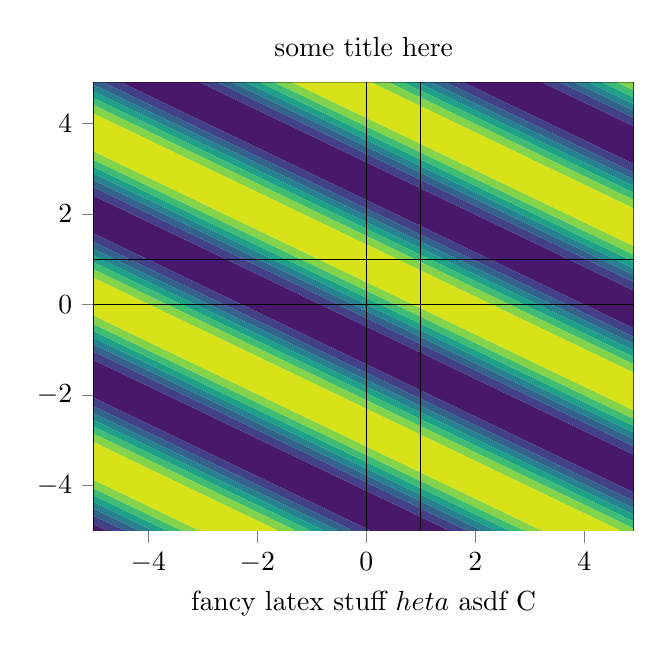
\begin{tikzpicture}

\definecolor{color0}{rgb}{0.282327,0.094955,0.417331}
\definecolor{color1}{rgb}{0.258965,0.251537,0.524736}
\definecolor{color2}{rgb}{0.19943,0.387607,0.554642}
\definecolor{color3}{rgb}{0.149039,0.508051,0.55725}
\definecolor{color4}{rgb}{0.120638,0.625828,0.533488}
\definecolor{color5}{rgb}{0.24607,0.73891,0.452024}
\definecolor{color6}{rgb}{0.515992,0.831158,0.294279}
\definecolor{color7}{rgb}{0.845561,0.887322,0.099702}

\begin{axis}[
title={some title here},
xlabel={fancy latex stuff $	heta$ asdf C},
xmin=-5, xmax=4.89999999999996,
ymin=-5, ymax=4.89999999999996,
xtick={-6,-4,-2,0,2,4,6},
xticklabels={,$-4$,$-2$,$0$,$2$,$4$,},
ytick={-6,-4,-2,0,2,4,6},
yticklabels={,$-4$,$-2$,$0$,$2$,$4$,},
tick align=outside,
tick pos=left,
x grid style={white!69.019607843137251!black},
y grid style={white!69.019607843137251!black}
]
\addplot [draw=none, fill=color0, colormap/viridis]
table{%
x                      y
-4.900000000000000e+00 -5.000000000000000e+00
-4.800000000000001e+00 -5.000000000000000e+00
-4.755576341188176e+00 -5.000000000000000e+00
-4.800000000000001e+00 -4.975329185975615e+00
-4.900000000000000e+00 -4.917262257847559e+00
-4.928556569754836e+00 -4.900000000000000e+00
-5.000000000000000e+00 -4.860410795697366e+00
-5.000000000000000e+00 -4.900000000000000e+00
-5.000000000000000e+00 -5.000000000000000e+00
-4.900000000000000e+00 -5.000000000000000e+00
};
\addplot [draw=none, fill=color0, colormap/viridis]
table{%
x                      y
-1.776356839400250e-14 -4.949302816499984e+00
+8.427479147698058e-02 -5.000000000000000e+00
+9.999999999998188e-02 -5.000000000000000e+00
+1.999999999999815e-01 -5.000000000000000e+00
+2.999999999999812e-01 -5.000000000000000e+00
+3.999999999999808e-01 -5.000000000000000e+00
+4.999999999999805e-01 -5.000000000000000e+00
+5.999999999999801e-01 -5.000000000000000e+00
+6.999999999999797e-01 -5.000000000000000e+00
+7.999999999999794e-01 -5.000000000000000e+00
+8.999999999999790e-01 -5.000000000000000e+00
+9.999999999999787e-01 -5.000000000000000e+00
+1.099999999999978e+00 -5.000000000000000e+00
+1.199999999999978e+00 -5.000000000000000e+00
+1.299999999999978e+00 -5.000000000000000e+00
+1.399999999999977e+00 -5.000000000000000e+00
+1.499999999999977e+00 -5.000000000000000e+00
+1.527880016017768e+00 -5.000000000000000e+00
+1.499999999999977e+00 -4.984496371609415e+00
+1.399999999999977e+00 -4.927529739870861e+00
+1.354388919974494e+00 -4.900000000000000e+00
+1.299999999999978e+00 -4.869819207970142e+00
+1.199999999999978e+00 -4.811052210670107e+00
+1.181733603002507e+00 -4.800000000000001e+00
+1.099999999999978e+00 -4.754747303405308e+00
+1.008940951963750e+00 -4.700000000000001e+00
+9.999999999999787e-01 -4.695020732254136e+00
+8.999999999999790e-01 -4.639221642433895e+00
+8.349074775162765e-01 -4.600000000000001e+00
+7.999999999999794e-01 -4.580599299370366e+00
+6.999999999999797e-01 -4.523174600954652e+00
+6.616290928826901e-01 -4.500000000000002e+00
+5.999999999999801e-01 -4.465821725280453e+00
+4.999999999999805e-01 -4.406528124552171e+00
+4.892181151039643e-01 -4.400000000000002e+00
+3.999999999999808e-01 -4.350634353092239e+00
+3.158303965913569e-01 -4.300000000000002e+00
+2.999999999999812e-01 -4.291188664439860e+00
+1.999999999999815e-01 -4.234976017245501e+00
+1.419890744000580e-01 -4.200000000000003e+00
+9.999999999998188e-02 -4.176676691933469e+00
-1.776356839400250e-14 -4.118776494755062e+00
-3.106855099739660e-02 -4.100000000000003e+00
-1.000000000000174e-01 -4.061794861895653e+00
-2.000000000000171e-01 -4.001954569717171e+00
-2.032259262905788e-01 -4.000000000000004e+00
-3.000000000000167e-01 -3.946487639132497e+00
-3.772312670207432e-01 -3.900000000000004e+00
-4.000000000000163e-01 -3.887333588079850e+00
-5.000000000000160e-01 -3.830691597290842e+00
-5.508731434326892e-01 -3.800000000000004e+00
-6.000000000000156e-01 -3.772727566219235e+00
-7.000000000000153e-01 -3.714333776189385e+00
-7.237016586098917e-01 -3.700000000000005e+00
-8.000000000000149e-01 -3.657737500280956e+00
-8.960725161073639e-01 -3.600000000000005e+00
-9.000000000000146e-01 -3.597811917549810e+00
-1.000000000000014e+00 -3.542305882190032e+00
-1.070242177487130e+00 -3.500000000000005e+00
-1.100000000000014e+00 -3.483454604235022e+00
-1.200000000000014e+00 -3.426366907383694e+00
-1.243677050402657e+00 -3.400000000000006e+00
-1.300000000000013e+00 -3.368750905485629e+00
-1.400000000000013e+00 -3.309844731450736e+00
-1.416267785305505e+00 -3.300000000000006e+00
-1.500000000000012e+00 -3.253648482476345e+00
-1.589217719093460e+00 -3.200000000000006e+00
-1.600000000000012e+00 -3.193996139569514e+00
-1.700000000000012e+00 -3.138087754110599e+00
-1.763200407361876e+00 -3.100000000000007e+00
-1.800000000000011e+00 -3.079550784433030e+00
-1.900000000000011e+00 -3.022000413013328e+00
-1.936420441326851e+00 -3.000000000000007e+00
-2.000000000000011e+00 -2.964745657653647e+00
-2.100000000000010e+00 -2.905307574134826e+00
-2.108764389932042e+00 -2.900000000000007e+00
-2.200000000000010e+00 -2.849526608025084e+00
-2.282315352899163e+00 -2.800000000000008e+00
-2.300000000000010e+00 -2.790157993179707e+00
-2.400000000000009e+00 -2.733831875337410e+00
-2.456103959791978e+00 -2.700000000000008e+00
-2.500000000000009e+00 -2.675621169228081e+00
-2.600000000000009e+00 -2.617590517091416e+00
-2.629101027256483e+00 -2.600000000000009e+00
-2.700000000000008e+00 -2.560710733536045e+00
-2.800000000000008e+00 -2.500720441105777e+00
-2.801188829612682e+00 -2.500000000000009e+00
-2.900000000000007e+00 -2.445370631777591e+00
-2.975363602484616e+00 -2.400000000000009e+00
-3.000000000000007e+00 -2.386296600192108e+00
-3.100000000000007e+00 -2.329536812164888e+00
-3.148950764972326e+00 -2.300000000000010e+00
-3.200000000000006e+00 -2.271664766679813e+00
-3.300000000000006e+00 -2.213135556486516e+00
-3.321716431057980e+00 -2.200000000000010e+00
-3.400000000000006e+00 -2.156645004962561e+00
-3.494240343788920e+00 -2.100000000000010e+00
-3.500000000000005e+00 -2.096791628068545e+00
-3.600000000000005e+00 -2.041179261561754e+00
-3.668360589081030e+00 -2.000000000000011e+00
-3.700000000000005e+00 -1.982411053891083e+00
-3.800000000000004e+00 -1.925201073818477e+00
-3.841738676388211e+00 -1.900000000000011e+00
-3.900000000000004e+00 -1.867680550745803e+00
-4.000000000000004e+00 -1.808633798329659e+00
-4.014264182718215e+00 -1.800000000000011e+00
-4.100000000000003e+00 -1.752547302794393e+00
-4.187372975174133e+00 -1.700000000000012e+00
-4.200000000000003e+00 -1.692969941056437e+00
-4.300000000000002e+00 -1.636951155710025e+00
-4.361304366981113e+00 -1.600000000000012e+00
-4.400000000000002e+00 -1.578500417649485e+00
-4.500000000000002e+00 -1.520823109347405e+00
-4.534465466830192e+00 -1.500000000000012e+00
-4.600000000000001e+00 -1.463667459581807e+00
-4.700000000000001e+00 -1.404083436073143e+00
-4.706741714353574e+00 -1.400000000000013e+00
-4.800000000000001e+00 -1.348416414820152e+00
-4.880457557115983e+00 -1.300000000000013e+00
-4.900000000000000e+00 -1.289125653047299e+00
-5.000000000000000e+00 -1.232684920432819e+00
-5.000000000000000e+00 -1.300000000000013e+00
-5.000000000000000e+00 -1.400000000000013e+00
-5.000000000000000e+00 -1.500000000000012e+00
-5.000000000000000e+00 -1.600000000000012e+00
-5.000000000000000e+00 -1.700000000000012e+00
-5.000000000000000e+00 -1.800000000000011e+00
-5.000000000000000e+00 -1.900000000000011e+00
-5.000000000000000e+00 -2.000000000000011e+00
-5.000000000000000e+00 -2.062679453070871e+00
-4.938079491008236e+00 -2.100000000000010e+00
-4.900000000000000e+00 -2.121158288096208e+00
-4.800000000000001e+00 -2.178794236300629e+00
-4.764899188910173e+00 -2.200000000000010e+00
-4.700000000000001e+00 -2.235982177688742e+00
-4.600000000000001e+00 -2.295518648778176e+00
-4.592600882429558e+00 -2.300000000000010e+00
-4.500000000000002e+00 -2.351222797514107e+00
-4.418938762085793e+00 -2.400000000000009e+00
-4.400000000000002e+00 -2.410538926728996e+00
-4.300000000000002e+00 -2.466942313886788e+00
-4.245186050692673e+00 -2.500000000000009e+00
-4.200000000000003e+00 -2.525092675645338e+00
-4.100000000000003e+00 -2.583212160866404e+00
-4.072230218044245e+00 -2.600000000000009e+00
-4.000000000000004e+00 -2.640022590704796e+00
-3.900169402010099e+00 -2.700000000000008e+00
-3.900000000000004e+00 -2.700094404525419e+00
-3.800000000000004e+00 -2.755385080677778e+00
-3.725899646742870e+00 -2.800000000000008e+00
-3.700000000000005e+00 -2.814404621901822e+00
-3.600000000000005e+00 -2.871244624521333e+00
-3.552349740213343e+00 -2.900000000000007e+00
-3.500000000000005e+00 -2.929054033611473e+00
-3.400000000000006e+00 -2.987675458376046e+00
-3.379626869199161e+00 -3.000000000000007e+00
-3.300000000000006e+00 -3.044094016621601e+00
-3.206998736592717e+00 -3.100000000000007e+00
-3.200000000000006e+00 -3.103898220376417e+00
-3.100000000000007e+00 -3.159582996824883e+00
-3.032912141382609e+00 -3.200000000000006e+00
-3.000000000000007e+00 -3.218294637600503e+00
-2.900000000000007e+00 -3.275587886401244e+00
-2.859572720383426e+00 -3.300000000000006e+00
-2.800000000000008e+00 -3.333043394386169e+00
-2.700000000000008e+00 -3.392185874730182e+00
-2.687091629717621e+00 -3.400000000000006e+00
-2.600000000000009e+00 -3.448197632211885e+00
-2.513874666191823e+00 -3.500000000000006e+00
-2.500000000000009e+00 -3.507723932368728e+00
-2.400000000000009e+00 -3.563817896854485e+00
-2.339978204181314e+00 -3.600000000000005e+00
-2.300000000000010e+00 -3.622209916018079e+00
-2.200000000000010e+00 -3.679973661712753e+00
-2.166857233457459e+00 -3.700000000000005e+00
-2.100000000000010e+00 -3.737061826480687e+00
-2.000000000000011e+00 -3.796745230249146e+00
-1.994627085749201e+00 -3.800000000000004e+00
-1.900000000000011e+00 -3.852334657714969e+00
-1.820798972032551e+00 -3.900000000000003e+00
-1.800000000000011e+00 -3.911572403533929e+00
-1.700000000000012e+00 -3.968091184280215e+00
-1.647099864288320e+00 -4.000000000000004e+00
-1.600000000000012e+00 -4.026151430993519e+00
-1.500000000000012e+00 -4.084403576748085e+00
-1.474205607406536e+00 -4.100000000000003e+00
-1.400000000000013e+00 -4.141110436342863e+00
-1.301994845380968e+00 -4.200000000000003e+00
-1.300000000000013e+00 -4.201111534251019e+00
-1.200000000000014e+00 -4.256506359091705e+00
-1.127773497376358e+00 -4.300000000000002e+00
-1.100000000000014e+00 -4.315444524699359e+00
-1.000000000000014e+00 -4.372404318053055e+00
-9.542792254646004e-01 -4.400000000000002e+00
-9.000000000000146e-01 -4.430120189570919e+00
-8.000000000000149e-01 -4.488879325471602e+00
-7.816202604586567e-01 -4.500000000000002e+00
-7.000000000000153e-01 -4.545190370280680e+00
-6.088364937622481e-01 -4.600000000000001e+00
-6.000000000000156e-01 -4.604921134036525e+00
-5.000000000000160e-01 -4.660714050417206e+00
-4.348001506318030e-01 -4.700000000000001e+00
-4.000000000000163e-01 -4.719341215831807e+00
-3.000000000000167e-01 -4.776758815563804e+00
-2.615184699404868e-01 -4.800000000000001e+00
-2.000000000000171e-01 -4.834117233647659e+00
-1.000000000000174e-01 -4.893402673322693e+00
-8.910370592381825e-02 -4.900000000000000e+00
-1.776356839400250e-14 -4.949302816499984e+00
};
\addplot [draw=none, fill=color0, colormap/viridis]
table{%
x                      y
+4.899999999999965e+00 -4.150716889691899e+00
+4.899999999999965e+00 -4.100000000000003e+00
+4.899999999999965e+00 -4.000000000000004e+00
+4.899999999999965e+00 -3.900000000000004e+00
+4.899999999999965e+00 -3.800000000000004e+00
+4.899999999999965e+00 -3.700000000000005e+00
+4.899999999999965e+00 -3.600000000000005e+00
+4.899999999999965e+00 -3.500000000000005e+00
+4.899999999999965e+00 -3.400000000000006e+00
+4.899999999999965e+00 -3.320285514683236e+00
+4.866427014711801e+00 -3.300000000000006e+00
+4.799999999999965e+00 -3.263175361568248e+00
+4.699999999999966e+00 -3.203524338792232e+00
+4.694181846546361e+00 -3.200000000000006e+00
+4.599999999999966e+00 -3.147909628896123e+00
+4.520390313378029e+00 -3.100000000000007e+00
+4.499999999999966e+00 -3.088654608899561e+00
+4.399999999999967e+00 -3.032161258427614e+00
+4.346679392794607e+00 -3.000000000000007e+00
+4.299999999999967e+00 -2.974081152575607e+00
+4.199999999999967e+00 -2.915858242151824e+00
+4.173771566338808e+00 -2.900000000000007e+00
+4.099999999999968e+00 -2.859128558089977e+00
+4.001593848609151e+00 -2.800000000000008e+00
+3.999999999999968e+00 -2.799111875173785e+00
+3.899999999999968e+00 -2.743740003042229e+00
+3.827361832643188e+00 -2.700000000000008e+00
+3.799999999999969e+00 -2.684783903997949e+00
+3.699999999999969e+00 -2.627850509828180e+00
+3.653855300381796e+00 -2.600000000000009e+00
+3.599999999999969e+00 -2.570114024954998e+00
+3.499999999999970e+00 -2.511385237511125e+00
+3.481182252245634e+00 -2.500000000000009e+00
+3.399999999999970e+00 -2.455050499101037e+00
+3.308432783232901e+00 -2.400000000000009e+00
+3.299999999999971e+00 -2.395303550240437e+00
+3.199999999999971e+00 -2.339534465909896e+00
+3.134385365706255e+00 -2.300000000000010e+00
+3.099999999999971e+00 -2.280888684073278e+00
+2.999999999999972e+00 -2.223498488417491e+00
+2.961090960665872e+00 -2.200000000000010e+00
+2.899999999999972e+00 -2.166118674114830e+00
+2.799999999999972e+00 -2.106864739635653e+00
+2.788661580010626e+00 -2.100000000000010e+00
+2.699999999999973e+00 -2.050939998918560e+00
+2.615318680396902e+00 -2.000000000000011e+00
+2.599999999999973e+00 -1.991473150915321e+00
+2.499999999999973e+00 -1.935291655821820e+00
+2.441462885295484e+00 -1.900000000000011e+00
+2.399999999999974e+00 -1.876968000439162e+00
+2.299999999999974e+00 -1.819103618886696e+00
+2.268388633465114e+00 -1.800000000000011e+00
+2.199999999999974e+00 -1.762094023763893e+00
+2.099999999999975e+00 -1.702294912112777e+00
+2.096212157114458e+00 -1.700000000000012e+00
+1.999999999999975e+00 -1.646795827932439e+00
+1.922253334051221e+00 -1.600000000000012e+00
+1.899999999999976e+00 -1.587619808461554e+00
+1.799999999999976e+00 -1.531010157910025e+00
+1.748596435855710e+00 -1.500000000000012e+00
+1.699999999999976e+00 -1.473020872444283e+00
+1.599999999999977e+00 -1.414664261093880e+00
+1.575750665241316e+00 -1.400000000000013e+00
+1.499999999999977e+00 -1.358038959281187e+00
+1.403421828954905e+00 -1.300000000000013e+00
+1.399999999999977e+00 -1.298093554412502e+00
+1.299999999999978e+00 -1.242616710322364e+00
+1.229238600818344e+00 -1.200000000000014e+00
+1.199999999999978e+00 -1.183742626071417e+00
+1.099999999999978e+00 -1.126688501256580e+00
+1.055788137231536e+00 -1.100000000000014e+00
+9.999999999999787e-01 -1.069046285895077e+00
+8.999999999999790e-01 -1.010178706449869e+00
+8.831794936980227e-01 -1.000000000000014e+00
+7.999999999999794e-01 -9.539523257691230e-01
+7.102731746416548e-01 -9.000000000000146e-01
+6.999999999999797e-01 -8.942793983271187e-01
+5.999999999999801e-01 -8.384013216350329e-01
+5.362764031410199e-01 -8.000000000000149e-01
+4.999999999999805e-01 -7.798406775074742e-01
+3.999999999999808e-01 -7.223251558518651e-01
+3.630401885728445e-01 -7.000000000000153e-01
+2.999999999999812e-01 -6.650431913882104e-01
+1.999999999999815e-01 -6.056451740635341e-01
+1.906776526677746e-01 -6.000000000000156e-01
+9.999999999998188e-02 -5.498329259909223e-01
+1.717195758091276e-02 -5.000000000000160e-01
-1.776356839400250e-14 -4.904429377515412e-01
-1.000000000000174e-01 -4.341482862113427e-01
-1.566312673853242e-01 -4.000000000000163e-01
-2.000000000000171e-01 -3.759130056681784e-01
-3.000000000000167e-01 -3.179185293565995e-01
-3.296451275214251e-01 -3.000000000000167e-01
-4.000000000000163e-01 -2.610105025467153e-01
-5.000000000000160e-01 -2.010618066276325e-01
-5.017522226900589e-01 -2.000000000000171e-01
-6.000000000000156e-01 -1.456795181840164e-01
-6.758800117829804e-01 -1.000000000000174e-01
-7.000000000000152e-01 -8.658329655650944e-02
-8.000000000000149e-01 -2.985617445253254e-02
-8.494823464827205e-01 -1.776356839400250e-14
-9.000000000000146e-01 +2.804137892707525e-02
-1.000000000000014e+00 +8.653303634740989e-02
-1.022265440603913e+00 +9.999999999998188e-02
-1.100000000000014e+00 +1.430529058468938e-01
-1.194746910819663e+00 +1.999999999999815e-01
-1.200000000000014e+00 +2.029263066394029e-01
-1.300000000000013e+00 +2.585091862594275e-01
-1.368880859507212e+00 +2.999999999999812e-01
-1.400000000000013e+00 +3.173004298150473e-01
-1.500000000000012e+00 +3.744765000867015e-01
-1.542274693449397e+00 +3.999999999999808e-01
-1.600000000000012e+00 +4.320234997388579e-01
-1.700000000000012e+00 +4.910312688341321e-01
-1.714818287705183e+00 +4.999999999999805e-01
-1.800000000000011e+00 +5.471481998276784e-01
-1.887883028443842e+00 +5.999999999999801e-01
-1.900000000000011e+00 +6.067463548259768e-01
-2.000000000000011e+00 +6.627345252544634e-01
-2.061828644954401e+00 +6.999999999999797e-01
-2.100000000000010e+00 +7.212091757266523e-01
-2.200000000000010e+00 +7.788512837911143e-01
-2.235006087192045e+00 +7.999999999999794e-01
-2.300000000000010e+00 +8.360344159004173e-01
-2.400000000000009e+00 +8.955779690556022e-01
-2.407301108365445e+00 +8.999999999999790e-01
-2.500000000000009e+00 +9.512765883432701e-01
-2.580971229762037e+00 +9.999999999999787e-01
-2.600000000000009e+00 +1.010588939548014e+00
-2.700000000000008e+00 +1.066997888638206e+00
-2.754721357408595e+00 +1.099999999999978e+00
-2.800000000000008e+00 +1.125143906803752e+00
-2.900000000000007e+00 +1.183269786277975e+00
-2.927674222015304e+00 +1.199999999999978e+00
-3.000000000000007e+00 +1.240075224008477e+00
-3.099742265554127e+00 +1.299999999999978e+00
-3.100000000000007e+00 +1.300143629545963e+00
-3.200000000000006e+00 +1.355439325475175e+00
-3.274009687618843e+00 +1.399999999999977e+00
-3.300000000000006e+00 +1.414454944420934e+00
-3.400000000000006e+00 +1.471300720948837e+00
-3.447556912490164e+00 +1.499999999999977e+00
-3.500000000000005e+00 +1.529105621471148e+00
-3.600000000000005e+00 +1.587733683905640e+00
-3.620276703150807e+00 +1.599999999999977e+00
-3.700000000000005e+00 +1.644147060018911e+00
-3.792912337467107e+00 +1.699999999999976e+00
-3.800000000000004e+00 +1.703947724127386e+00
-3.900000000000004e+00 +1.759637712795453e+00
-3.966996510521716e+00 +1.799999999999976e+00
-4.000000000000004e+00 +1.818345281850114e+00
-4.100000000000003e+00 +1.875644524381013e+00
-4.140333148355388e+00 +1.899999999999975e+00
-4.200000000000003e+00 +1.933095352577912e+00
-4.300000000000002e+00 +1.992244723514373e+00
-4.312811042006645e+00 +1.999999999999975e+00
-4.400000000000002e+00 +2.048251101254622e+00
-4.486035791633498e+00 +2.099999999999975e+00
-4.500000000000003e+00 +2.107773725877045e+00
-4.600000000000001e+00 +2.163873101868585e+00
-4.659929739395761e+00 +2.199999999999974e+00
-4.700000000000001e+00 +2.222260894429635e+00
-4.800000000000001e+00 +2.280030861930972e+00
-4.833047821665329e+00 +2.299999999999974e+00
-4.900000000000000e+00 +2.337114169115745e+00
-5.000000000000000e+00 +2.396804726417623e+00
-5.000000000000000e+00 +2.299999999999974e+00
-5.000000000000000e+00 +2.199999999999974e+00
-5.000000000000000e+00 +2.099999999999975e+00
-5.000000000000000e+00 +1.999999999999975e+00
-5.000000000000000e+00 +1.899999999999975e+00
-5.000000000000000e+00 +1.799999999999976e+00
-5.000000000000000e+00 +1.699999999999976e+00
-5.000000000000000e+00 +1.599999999999977e+00
-5.000000000000000e+00 +1.564797820943346e+00
-4.900000000000000e+00 +1.505366768236256e+00
-4.891137783051183e+00 +1.499999999999977e+00
-4.800000000000001e+00 +1.449580312761107e+00
-4.717594763626781e+00 +1.399999999999977e+00
-4.700000000000001e+00 +1.390207947303543e+00
-4.600000000000001e+00 +1.333887351163771e+00
-4.543803591572605e+00 +1.299999999999978e+00
-4.500000000000002e+00 +1.275672332755968e+00
-4.400000000000002e+00 +1.217648028729651e+00
-4.370803577360472e+00 +1.199999999999978e+00
-4.300000000000002e+00 +1.160763289070119e+00
-4.200000000000003e+00 +1.100780296007432e+00
-4.198712389519996e+00 +1.099999999999978e+00
-4.100000000000003e+00 +1.045424787219736e+00
-4.024545861297177e+00 +9.999999999999786e-01
-4.000000000000004e+00 +9.863468617280037e-01
-3.900000000000004e+00 +9.295928059032282e-01
-3.850956036413105e+00 +8.999999999999790e-01
-3.800000000000004e+00 +8.717162843194126e-01
-3.700000000000005e+00 +8.131936638666477e-01
-3.678187312085649e+00 +7.999999999999794e-01
-3.600000000000005e+00 +7.566979676390991e-01
-3.505670847112283e+00 +6.999999999999797e-01
-3.500000000000005e+00 +6.968410769187044e-01
-3.400000000000006e+00 +6.412338847898599e-01
-3.331548197154496e+00 +5.999999999999801e-01
-3.300000000000006e+00 +5.824616347938675e-01
-3.200000000000006e+00 +5.252576051928566e-01
-3.158167346655080e+00 +4.999999999999805e-01
-3.100000000000007e+00 +4.677324360374510e-01
-3.000000000000007e+00 +4.086925244019825e-01
-2.985638666283354e+00 +3.999999999999808e-01
-2.900000000000007e+00 +3.526006880563374e-01
-2.812537603960482e+00 +2.999999999999812e-01
-2.800000000000007e+00 +2.930196774986429e-01
-2.700000000000008e+00 +2.370062644627040e-01
-2.638603716016036e+00 +1.999999999999815e-01
-2.600000000000009e+00 +1.785513302713314e-01
-2.500000000000009e+00 +1.208801988835203e-01
-2.465439748434270e+00 +9.999999999998188e-02
-2.400000000000009e+00 +6.371972654173416e-02
-2.300000000000010e+00 +4.142804770421367e-03
-2.293160206533860e+00 -1.776356839400250e-14
-2.200000000000010e+00 -5.152976131660394e-02
-2.119452386891474e+00 -1.000000000000174e-01
-2.100000000000010e+00 -1.108243116087589e-01
-2.000000000000011e+00 -1.672594668574258e-01
-1.945714432990670e+00 -2.000000000000171e-01
-1.900000000000011e+00 -2.253850194228014e-01
-1.800000000000011e+00 -2.835410266143170e-01
-1.772775552753802e+00 -3.000000000000167e-01
-1.700000000000012e+00 -3.403229431122325e-01
-1.600673455595939e+00 -4.000000000000163e-01
-1.600000000000012e+00 -4.003752895633026e-01
-1.500000000000012e+00 -4.556946373919571e-01
-1.426417026899344e+00 -5.000000000000160e-01
-1.400000000000013e+00 -5.146917757380784e-01
-1.300000000000013e+00 -5.715647571425563e-01
-1.252882437076665e+00 -6.000000000000156e-01
-1.200000000000014e+00 -6.293484147677312e-01
-1.100000000000014e+00 -6.880077518528557e-01
-1.080177159971654e+00 -7.000000000000153e-01
-1.000000000000014e+00 -7.443967113473990e-01
-9.075061801211102e-01 -8.000000000000149e-01
-9.000000000000147e-01 -8.041806975125194e-01
-8.000000000000149e-01 -8.598952447210029e-01
-7.334334195082115e-01 -9.000000000000146e-01
-7.000000000000153e-01 -9.185836290971071e-01
-6.000000000000156e-01 -9.759111122076473e-01
-5.601098949757422e-01 -1.000000000000014e+00
-5.000000000000160e-01 -1.033339890769108e+00
-4.000000000000163e-01 -1.092521728102531e+00
-3.876470645689182e-01 -1.100000000000014e+00
-3.000000000000167e-01 -1.148502758080147e+00
-2.143856294757275e-01 -1.200000000000014e+00
-2.000000000000171e-01 -1.208008064573603e+00
-1.000000000000174e-01 -1.264132938005137e+00
-4.050352802876402e-02 -1.300000000000013e+00
-1.776356839400250e-14 -1.322500816170226e+00
+9.999999999998188e-02 -1.380300098867735e+00
+1.326009448611845e-01 -1.400000000000013e+00
+1.999999999999815e-01 -1.437360518683299e+00
+2.999999999999812e-01 -1.497084781359210e+00
+3.048121397802503e-01 -1.500000000000012e+00
+3.999999999999808e-01 -1.552642306855883e+00
+4.786864106250022e-01 -1.600000000000012e+00
+4.999999999999805e-01 -1.611858255791510e+00
+5.999999999999801e-01 -1.668409124763431e+00
+6.523706129930804e-01 -1.700000000000012e+00
+6.999999999999797e-01 -1.726444313200259e+00
+7.999999999999794e-01 -1.784733348300140e+00
+8.252477479398229e-01 -1.800000000000011e+00
+8.999999999999790e-01 -1.841411407841911e+00
+9.975002051864562e-01 -1.900000000000011e+00
+9.999999999999787e-01 -1.901392839824822e+00
+1.099999999999978e+00 -1.956816627113848e+00
+1.171708092205226e+00 -2.000000000000011e+00
+1.199999999999978e+00 -2.015732164103986e+00
+1.299999999999978e+00 -2.072725268168277e+00
+1.345186894121861e+00 -2.100000000000010e+00
+1.399999999999977e+00 -2.130415129754054e+00
+1.499999999999977e+00 -2.189212559627534e+00
+1.517828089161752e+00 -2.200000000000010e+00
+1.599999999999977e+00 -2.245493707583555e+00
+1.690655132507492e+00 -2.300000000000010e+00
+1.699999999999976e+00 -2.305204048389289e+00
+1.799999999999976e+00 -2.361027036590443e+00
+1.864677501904586e+00 -2.400000000000009e+00
+1.899999999999975e+00 -2.419630711690609e+00
+1.999999999999975e+00 -2.477082890061684e+00
+2.037943127158005e+00 -2.500000000000009e+00
+2.099999999999975e+00 -2.534414310377466e+00
+2.199999999999974e+00 -2.593739503739077e+00
+2.210339447977442e+00 -2.600000000000009e+00
+2.299999999999974e+00 -2.649608609300326e+00
+2.383762862454263e+00 -2.700000000000008e+00
+2.399999999999974e+00 -2.709037445191730e+00
+2.499999999999973e+00 -2.765274903871139e+00
+2.557592657671481e+00 -2.800000000000008e+00
+2.599999999999973e+00 -2.823554851396702e+00
+2.699999999999973e+00 -2.881483574165900e+00
+2.730637041027213e+00 -2.900000000000007e+00
+2.799999999999972e+00 -2.938442936345833e+00
+2.899999999999972e+00 -2.998316027368354e+00
+2.902779203231701e+00 -3.000000000000007e+00
+2.999999999999972e+00 -3.053757348607154e+00
+3.076821592925358e+00 -3.100000000000007e+00
+3.099999999999971e+00 -3.112893902622699e+00
+3.199999999999971e+00 -3.169561651101907e+00
+3.250451505260657e+00 -3.200000000000006e+00
+3.299999999999971e+00 -3.227505568237087e+00
+3.399999999999970e+00 -3.285928969503184e+00
+3.423266277416691e+00 -3.300000000000006e+00
+3.499999999999970e+00 -3.342502127516532e+00
+3.595670602738959e+00 -3.400000000000006e+00
+3.599999999999969e+00 -3.402411922287464e+00
+3.699999999999969e+00 -3.457941207642785e+00
+3.769829458738937e+00 -3.500000000000005e+00
+3.799999999999969e+00 -3.516774321319941e+00
+3.899999999999968e+00 -3.573888756871989e+00
+3.943251914521368e+00 -3.600000000000005e+00
+3.999999999999968e+00 -3.631483880985049e+00
+4.099999999999968e+00 -3.690420794040924e+00
+4.115828386139696e+00 -3.700000000000005e+00
+4.199999999999967e+00 -3.746593044290716e+00
+4.288813056850635e+00 -3.800000000000004e+00
+4.299999999999967e+00 -3.806228992160253e+00
+4.399999999999967e+00 -3.862161517511894e+00
+4.462784528461064e+00 -3.900000000000004e+00
+4.499999999999966e+00 -3.920679631537028e+00
+4.599999999999966e+00 -3.978257759280875e+00
+4.635991675461155e+00 -4.000000000000004e+00
+4.699999999999966e+00 -4.035490843852289e+00
+4.799999999999965e+00 -4.094960838579672e+00
+4.808320820208307e+00 -4.100000000000003e+00
+4.899999999999965e+00 -4.150716889691899e+00
};
\addplot [draw=none, fill=color0, colormap/viridis]
table{%
x                      y
+4.899999999999965e+00 -5.238464209980110e-01
+4.899999999999965e+00 -5.000000000000160e-01
+4.899999999999965e+00 -4.000000000000163e-01
+4.899999999999965e+00 -3.000000000000167e-01
+4.899999999999965e+00 -2.000000000000171e-01
+4.899999999999965e+00 -1.000000000000174e-01
+4.899999999999965e+00 -1.776356839400250e-14
+4.899999999999965e+00 +9.999999999998188e-02
+4.899999999999965e+00 +1.999999999999815e-01
+4.899999999999965e+00 +2.999999999999812e-01
+4.899999999999965e+00 +3.082424883532625e-01
+4.799999999999965e+00 +3.643929176336536e-01
+4.740937003275866e+00 +3.999999999999808e-01
+4.699999999999966e+00 +4.227408359877992e-01
+4.599999999999966e+00 +4.805695008014276e-01
+4.567846170653185e+00 +4.999999999999805e-01
+4.499999999999966e+00 +5.376069810567297e-01
+4.399999999999967e+00 +5.973650263431581e-01
+4.395650645873384e+00 +5.999999999999801e-01
+4.299999999999967e+00 +6.528961747963645e-01
+4.221738212515910e+00 +6.999999999999797e-01
+4.199999999999967e+00 +7.120941018157863e-01
+4.099999999999968e+00 +7.686715015636566e-01
+4.048066333846666e+00 +7.999999999999794e-01
+3.999999999999968e+00 +8.266859718216025e-01
+3.899999999999968e+00 +8.850055071848189e-01
+3.875203355177506e+00 +8.999999999999790e-01
+3.799999999999969e+00 +9.416597547367793e-01
+3.702916424413982e+00 +9.999999999999787e-01
+3.699999999999969e+00 +1.001624926315697e+00
+3.599999999999969e+00 +1.057072660332528e+00
+3.528719667052399e+00 +1.099999999999978e+00
+3.499999999999970e+00 +1.115969487827512e+00
+3.399999999999970e+00 +1.172990133348279e+00
+3.355253655620475e+00 +1.199999999999978e+00
+3.299999999999971e+00 +1.230658489937640e+00
+3.199999999999971e+00 +1.289487581493817e+00
+3.182627152672714e+00 +1.299999999999978e+00
+3.099999999999971e+00 +1.345744010517646e+00
+3.009764328364267e+00 +1.399999999999977e+00
+2.999999999999972e+00 +1.405437465159222e+00
+2.899999999999972e+00 +1.461285317166834e+00
+2.835753512487307e+00 +1.499999999999977e+00
+2.799999999999972e+00 +1.519869570398821e+00
+2.699999999999973e+00 +1.577350338513770e+00
+2.662501161736759e+00 +1.599999999999977e+00
+2.599999999999973e+00 +1.634659437073235e+00
+2.499999999999973e+00 +1.694017499128927e+00
+2.490120089680183e+00 +1.699999999999976e+00
+2.399999999999974e+00 +1.749860942428131e+00
+2.316659537970594e+00 +1.799999999999976e+00
+2.299999999999974e+00 +1.809272244722251e+00
+2.199999999999974e+00 +1.865535517075678e+00
+2.142841735177823e+00 +1.899999999999975e+00
+2.099999999999975e+00 +1.923795304295317e+00
+1.999999999999975e+00 +1.981753704669264e+00
+1.969811128468722e+00 +1.999999999999975e+00
+1.899999999999976e+00 +2.038689896805313e+00
+1.799999999999976e+00 +2.098597111592837e+00
+1.797684793672142e+00 +2.099999999999975e+00
+1.699999999999976e+00 +2.154011788856501e+00
+1.623603859098340e+00 +2.199999999999974e+00
+1.599999999999977e+00 +2.213130139082184e+00
+1.499999999999977e+00 +2.269824685566937e+00
+1.449986393895277e+00 +2.299999999999974e+00
+1.399999999999977e+00 +2.327747676546621e+00
+1.299999999999978e+00 +2.386201884939848e+00
+1.277185919603113e+00 +2.399999999999974e+00
+1.199999999999978e+00 +2.442750991409414e+00
+1.104746775084618e+00 +2.499999999999973e+00
+1.099999999999978e+00 +2.502644360170838e+00
+9.999999999999787e-01 +2.558197834859798e+00
+9.305991608818533e-01 +2.599999999999973e+00
+8.999999999999790e-01 +2.617012050645082e+00
+7.999999999999794e-01 +2.674154304773605e+00
+7.571896235502436e-01 +2.699999999999973e+00
+6.999999999999797e-01 +2.731727708040726e+00
+5.999999999999801e-01 +2.790696601625985e+00
+5.846279910929026e-01 +2.799999999999972e+00
+4.999999999999805e-01 +2.846843883828340e+00
+4.116071808993932e-01 +2.899999999999972e+00
+3.999999999999808e-01 +2.906462774224075e+00
+2.999999999999812e-01 +2.962420414614909e+00
+2.376473789071450e-01 +2.999999999999972e+00
+1.999999999999815e-01 +3.020918911518820e+00
+9.999999999998188e-02 +3.078525916532463e+00
+6.445363914296884e-02 +3.099999999999971e+00
-1.776356839400250e-14 +3.135736455209698e+00
-1.000000000000174e-01 +3.195239650106983e+00
-1.078601039969849e-01 +3.199999999999971e+00
-2.000000000000171e-01 +3.250969779758133e+00
-2.814846297814597e-01 +3.299999999999971e+00
-3.000000000000167e-01 +3.310303660501718e+00
-4.000000000000163e-01 +3.366680914021708e+00
-4.552494814184643e-01 +3.399999999999970e+00
-5.000000000000160e-01 +3.424851684962694e+00
-6.000000000000156e-01 +3.482941125661813e+00
-6.282192600446808e-01 +3.499999999999970e+00
-7.000000000000153e-01 +3.539775011812989e+00
-8.000000000000149e-01 +3.599832903007818e+00
-8.002757102289653e-01 +3.599999999999969e+00
-9.000000000000146e-01 +3.655129929859736e+00
-9.745268344417320e-01 +3.699999999999969e+00
-1.000000000000014e+00 +3.714167900541279e+00
-1.100000000000014e+00 +3.770980773469497e+00
-1.148089341296601e+00 +3.799999999999969e+00
-1.200000000000014e+00 +3.828811366918603e+00
-1.300000000000013e+00 +3.887401603453537e+00
-1.320826685998178e+00 +3.899999999999968e+00
-1.400000000000013e+00 +3.943844510825099e+00
-1.493419570333925e+00 +3.999999999999968e+00
-1.500000000000013e+00 +4.003665345987575e+00
-1.600000000000012e+00 +4.059325632105309e+00
-1.667517546461073e+00 +4.099999999999968e+00
-1.700000000000012e+00 +4.118056404569638e+00
-1.800000000000011e+00 +4.175321490778918e+00
-1.840870044753881e+00 +4.199999999999967e+00
-1.900000000000011e+00 +4.232798987629286e+00
-2.000000000000011e+00 +4.291909091396122e+00
-2.013366157241192e+00 +4.299999999999967e+00
-2.100000000000010e+00 +4.347946126434889e+00
-2.186546536203143e+00 +4.399999999999967e+00
-2.200000000000010e+00 +4.407489696570106e+00
-2.300000000000010e+00 +4.463558234269006e+00
-2.360454811883444e+00 +4.499999999999966e+00
-2.400000000000009e+00 +4.521970112896211e+00
-2.500000000000009e+00 +4.579704624332534e+00
-2.533589354628411e+00 +4.599999999999966e+00
-2.600000000000009e+00 +4.636815613349553e+00
-2.700000000000008e+00 +4.696465405146729e+00
-2.705835093807673e+00 +4.699999999999966e+00
-2.800000000000008e+00 +4.752081076164384e+00
-2.879625236337350e+00 +4.799999999999965e+00
-2.900000000000007e+00 +4.811336752846580e+00
-3.000000000000007e+00 +4.867829136572729e+00
-3.053336605995173e+00 +4.899999999999965e+00
-3.100000000000007e+00 +4.899999999999965e+00
-3.200000000000006e+00 +4.899999999999965e+00
-3.300000000000006e+00 +4.899999999999965e+00
-3.400000000000006e+00 +4.899999999999965e+00
-3.500000000000005e+00 +4.899999999999965e+00
-3.600000000000005e+00 +4.899999999999965e+00
-3.700000000000005e+00 +4.899999999999965e+00
-3.800000000000004e+00 +4.899999999999965e+00
-3.900000000000004e+00 +4.899999999999965e+00
-4.000000000000004e+00 +4.899999999999965e+00
-4.100000000000003e+00 +4.899999999999965e+00
-4.200000000000003e+00 +4.899999999999965e+00
-4.300000000000002e+00 +4.899999999999965e+00
-4.400000000000002e+00 +4.899999999999965e+00
-4.497237803679572e+00 +4.899999999999965e+00
-4.400000000000002e+00 +4.846233325004766e+00
-4.323194002336837e+00 +4.799999999999965e+00
-4.300000000000002e+00 +4.787097437671054e+00
-4.200000000000003e+00 +4.730428707760050e+00
-4.149564545859586e+00 +4.699999999999966e+00
-4.100000000000003e+00 +4.672485557012793e+00
-4.000000000000004e+00 +4.614061027486486e+00
-3.976750297342616e+00 +4.599999999999966e+00
-3.900000000000004e+00 +4.557488750321228e+00
-3.804344696819767e+00 +4.499999999999966e+00
-3.800000000000004e+00 +4.497579557118122e+00
-3.700000000000005e+00 +4.442049385874667e+00
-3.630186252531613e+00 +4.399999999999967e+00
-3.600000000000005e+00 +4.383216964301226e+00
-3.500000000000005e+00 +4.326101509939605e+00
-3.456764269869121e+00 +4.299999999999967e+00
-3.400000000000006e+00 +4.268507181318815e+00
-3.300000000000006e+00 +4.209569097030086e+00
-3.284188341713566e+00 +4.199999999999967e+00
-3.200000000000006e+00 +4.153397761192000e+00
-3.111202347447562e+00 +4.099999999999968e+00
-3.100000000000007e+00 +4.093762438018967e+00
-3.000000000000007e+00 +4.037828992874399e+00
-2.937231303218399e+00 +3.999999999999968e+00
-2.900000000000007e+00 +3.979311597294773e+00
-2.800000000000008e+00 +3.921732411967959e+00
-2.764024647239577e+00 +3.899999999999968e+00
-2.700000000000008e+00 +3.864500153104506e+00
-2.600000000000009e+00 +3.805028942478984e+00
-2.591696066553121e+00 +3.799999999999969e+00
-2.500000000000009e+00 +3.749273840693212e+00
-2.418107676309609e+00 +3.699999999999970e+00
-2.400000000000009e+00 +3.689922897682525e+00
-2.300000000000010e+00 +3.633570763221356e+00
-2.244331155600845e+00 +3.599999999999969e+00
-2.200000000000010e+00 +3.575380375266282e+00
-2.100000000000010e+00 +3.517319812825870e+00
-2.071347972174799e+00 +3.499999999999970e+00
-2.000000000000011e+00 +3.460463380857205e+00
-1.900000000000011e+00 +3.400438695872113e+00
-1.899276121125750e+00 +3.399999999999970e+00
-1.800000000000011e+00 +3.345115740872342e+00
-1.725062502248285e+00 +3.299999999999971e+00
-1.700000000000012e+00 +3.286060056216994e+00
-1.600000000000012e+00 +3.229273259810951e+00
-1.551487884057894e+00 +3.199999999999971e+00
-1.500000000000012e+00 +3.171422304240159e+00
-1.400000000000013e+00 +3.112862045232135e+00
-1.378736627341974e+00 +3.099999999999971e+00
-1.300000000000013e+00 +3.056395733963248e+00
-1.206177623274401e+00 +2.999999999999971e+00
-1.200000000000014e+00 +2.996558913372891e+00
-1.100000000000014e+00 +2.940922166607550e+00
-1.032068708025690e+00 +2.899999999999972e+00
-1.000000000000014e+00 +2.882173005120820e+00
-9.000000000000146e-01 +2.824934988285395e+00
-8.587036399147288e-01 +2.799999999999972e+00
-8.000000000000149e-01 +2.767436356037661e+00
-7.000000000000153e-01 +2.708357371934649e+00
-6.861930885838743e-01 +2.699999999999973e+00
-6.000000000000156e-01 +2.652296040715444e+00
-5.130478743614290e-01 +2.599999999999973e+00
-5.000000000000160e-01 +2.592735871249341e+00
-4.000000000000163e-01 +2.536691773125702e+00
-3.391282435443840e-01 +2.499999999999973e+00
-3.000000000000167e-01 +2.478260805893976e+00
-2.000000000000171e-01 +2.420554393914590e+00
-1.659806554423275e-01 +2.399999999999974e+00
-1.000000000000174e-01 +2.363421466571323e+00
-1.776356839400250e-14 +2.303803981753508e+00
+6.280070071423049e-03 +2.299999999999974e+00
+9.999999999998188e-02 +2.248163086201517e+00
+1.800337150535495e-01 +2.199999999999974e+00
+1.999999999999815e-01 +2.188890174852363e+00
+2.999999999999812e-01 +2.132423163366024e+00
+3.537568707422168e-01 +2.099999999999975e+00
+3.999999999999808e-01 +2.074322488571714e+00
+4.999999999999805e-01 +2.016129858274887e+00
+5.266787518979079e-01 +1.999999999999975e+00
+5.999999999999801e-01 +1.959376534040389e+00
+6.988222441967377e-01 +1.899999999999975e+00
+6.999999999999797e-01 +1.899343709642831e+00
+7.999999999999794e-01 +1.843995610065063e+00
+8.730653093065441e-01 +1.799999999999976e+00
+8.999999999999789e-01 +1.785020936756196e+00
+9.999999999999787e-01 +1.728114885178008e+00
+1.046584540216522e+00 +1.699999999999976e+00
+1.099999999999978e+00 +1.670357050175658e+00
+1.199999999999978e+00 +1.611659695710136e+00
+1.219272174946574e+00 +1.599999999999977e+00
+1.299999999999978e+00 +1.555300417020427e+00
+1.391986120267430e+00 +1.499999999999977e+00
+1.399999999999977e+00 +1.495536705000305e+00
+1.499999999999977e+00 +1.439792304129844e+00
+1.566045007968736e+00 +1.399999999999977e+00
+1.599999999999977e+00 +1.381127240560547e+00
+1.699999999999976e+00 +1.323765428341175e+00
+1.739352592266102e+00 +1.299999999999978e+00
+1.799999999999976e+00 +1.266363453076615e+00
+1.899999999999975e+00 +1.207142149558144e+00
+1.911797112056403e+00 +1.199999999999978e+00
+1.999999999999975e+00 +1.151191932439697e+00
+2.085103141370707e+00 +1.099999999999978e+00
+2.099999999999975e+00 +1.091707678129509e+00
+2.199999999999974e+00 +1.035551809877516e+00
+2.258970842576159e+00 +9.999999999999787e-01
+2.299999999999974e+00 +9.772081394815728e-01
+2.399999999999974e+00 +9.193732213932619e-01
+2.432058772220136e+00 +8.999999999999790e-01
+2.499999999999973e+00 +8.623406232631169e-01
+2.599999999999973e+00 +8.025753881240629e-01
+2.604250961999110e+00 +7.999999999999794e-01
+2.699999999999973e+00 +7.470498534342987e-01
+2.778171517285115e+00 +6.999999999999797e-01
+2.799999999999972e+00 +6.878557619651019e-01
+2.899999999999972e+00 +6.312727157680293e-01
+2.951840773166293e+00 +5.999999999999801e-01
+2.999999999999972e+00 +5.732626548640205e-01
+3.099999999999971e+00 +5.149366282522205e-01
+3.124700739036145e+00 +4.999999999999805e-01
+3.199999999999971e+00 +4.582874485091959e-01
+3.296995006628169e+00 +3.999999999999808e-01
+3.299999999999971e+00 +3.983257376280626e-01
+3.399999999999970e+00 +3.428729070734328e-01
+3.471189395303285e+00 +2.999999999999812e-01
+3.499999999999970e+00 +2.839800614515408e-01
+3.599999999999969e+00 +2.269535543910540e-01
+3.644652684607954e+00 +1.999999999999815e-01
+3.699999999999969e+00 +1.692897746092197e-01
+3.799999999999969e+00 +1.104539446161313e-01
+3.817276060718728e+00 +9.999999999998188e-02
+3.899999999999968e+00 +5.420277643440384e-02
+3.990146500104387e+00 -1.776356839400251e-14
+3.999999999999968e+00 -5.487084348867975e-03
+4.099999999999968e+00 -6.134022805456845e-02
+4.164154857094941e+00 -1.000000000000174e-01
+4.199999999999967e+00 -1.199203478113481e-01
+4.299999999999967e+00 -1.774072005642215e-01
+4.337404382709806e+00 -2.000000000000171e-01
+4.399999999999967e+00 -2.347115484867531e-01
+4.499999999999966e+00 -2.940766058762787e-01
+4.509782209450576e+00 -3.000000000000167e-01
+4.599999999999966e+00 -3.499145875514902e-01
+4.683250664882309e+00 -4.000000000000163e-01
+4.699999999999966e+00 -4.093221582122741e-01
+4.799999999999965e+00 -4.655909244055812e-01
+4.857065915386135e+00 -5.000000000000160e-01
+4.899999999999965e+00 -5.238464209980110e-01
};
\addplot [draw=none, fill=color0, colormap/viridis]
table{%
x                      y
+4.799999999999965e+00 +3.162041598899869e+00
+4.899999999999965e+00 +3.102235277409876e+00
+4.899999999999965e+00 +3.199999999999971e+00
+4.899999999999965e+00 +3.299999999999971e+00
+4.899999999999965e+00 +3.399999999999970e+00
+4.899999999999965e+00 +3.499999999999970e+00
+4.899999999999965e+00 +3.599999999999969e+00
+4.899999999999965e+00 +3.699999999999969e+00
+4.899999999999965e+00 +3.799999999999969e+00
+4.899999999999965e+00 +3.899999999999968e+00
+4.899999999999965e+00 +3.934362227282730e+00
+4.799999999999965e+00 +3.993680444674127e+00
+4.789562920016321e+00 +3.999999999999968e+00
+4.699999999999966e+00 +4.049554996719602e+00
+4.616147387523576e+00 +4.099999999999968e+00
+4.599999999999967e+00 +4.108987553880925e+00
+4.499999999999966e+00 +4.165219533933135e+00
+4.442315047045799e+00 +4.199999999999967e+00
+4.399999999999967e+00 +4.223503760254649e+00
+4.299999999999967e+00 +4.281426184300631e+00
+4.269267739735118e+00 +4.299999999999967e+00
+4.199999999999967e+00 +4.338390464055958e+00
+4.099999999999968e+00 +4.398256312753557e+00
+4.097122218340621e+00 +4.399999999999967e+00
+3.999999999999968e+00 +4.453703288812028e+00
+3.923088009386688e+00 +4.499999999999966e+00
+3.899999999999968e+00 +4.512843706351440e+00
+3.799999999999969e+00 +4.569505767279372e+00
+3.749455455278266e+00 +4.599999999999966e+00
+3.699999999999969e+00 +4.627454125756971e+00
+3.599999999999969e+00 +4.685870988576363e+00
+3.576637648545810e+00 +4.699999999999966e+00
+3.499999999999970e+00 +4.742449251243972e+00
+3.404240713220321e+00 +4.799999999999965e+00
+3.399999999999970e+00 +4.802362532184165e+00
+3.299999999999971e+00 +4.857886683686941e+00
+3.230079471285829e+00 +4.899999999999965e+00
+3.199999999999971e+00 +4.899999999999965e+00
+3.099999999999971e+00 +4.899999999999965e+00
+2.999999999999972e+00 +4.899999999999965e+00
+2.899999999999972e+00 +4.899999999999965e+00
+2.799999999999972e+00 +4.899999999999965e+00
+2.699999999999973e+00 +4.899999999999965e+00
+2.599999999999973e+00 +4.899999999999965e+00
+2.499999999999973e+00 +4.899999999999965e+00
+2.399999999999974e+00 +4.899999999999965e+00
+2.299999999999974e+00 +4.899999999999965e+00
+2.199999999999974e+00 +4.899999999999965e+00
+2.099999999999975e+00 +4.899999999999965e+00
+1.999999999999975e+00 +4.899999999999965e+00
+1.899999999999975e+00 +4.899999999999965e+00
+1.799999999999976e+00 +4.899999999999965e+00
+1.786441591291871e+00 +4.899999999999965e+00
+1.799999999999976e+00 +4.892451940839085e+00
+1.899999999999975e+00 +4.836377072341128e+00
+1.960346925573251e+00 +4.799999999999965e+00
+1.999999999999975e+00 +4.777970138372065e+00
+2.099999999999975e+00 +4.720228348123552e+00
+2.133478089108833e+00 +4.699999999999966e+00
+2.199999999999974e+00 +4.663123041945660e+00
+2.299999999999974e+00 +4.603464881389319e+00
+2.305719946279803e+00 +4.599999999999966e+00
+2.399999999999974e+00 +4.547855744520058e+00
+2.479519542992507e+00 +4.499999999999966e+00
+2.499999999999973e+00 +4.488604532288942e+00
+2.599999999999973e+00 +4.432105576183671e+00
+2.653227859641724e+00 +4.399999999999967e+00
+2.699999999999973e+00 +4.374029847924852e+00
+2.799999999999972e+00 +4.315800493104209e+00
+2.826132694916792e+00 +4.299999999999967e+00
+2.899999999999972e+00 +4.259075840282257e+00
+2.998317696678239e+00 +4.199999999999967e+00
+2.999999999999972e+00 +4.199062592757632e+00
+3.099999999999971e+00 +4.143685661153220e+00
+3.172547361091145e+00 +4.099999999999968e+00
+3.199999999999971e+00 +4.084733515203558e+00
+3.299999999999971e+00 +4.027794301816328e+00
+3.346051190769565e+00 +3.999999999999968e+00
+3.399999999999970e+00 +3.970062360790963e+00
+3.499999999999970e+00 +3.911326883586389e+00
+3.518721134522160e+00 +3.899999999999968e+00
+3.599999999999969e+00 +3.854997367993772e+00
+3.691478163859683e+00 +3.799999999999969e+00
+3.699999999999969e+00 +3.795253986816141e+00
+3.799999999999969e+00 +3.739479649166680e+00
+3.865523140236345e+00 +3.699999999999969e+00
+3.899999999999968e+00 +3.680837970982414e+00
+3.999999999999968e+00 +3.623441734595724e+00
+4.038814740411367e+00 +3.599999999999969e+00
+4.099999999999968e+00 +3.566066636708172e+00
+4.199999999999967e+00 +3.506805757494071e+00
+4.211240899083586e+00 +3.499999999999970e+00
+4.299999999999967e+00 +3.450886438841358e+00
+4.384591645609567e+00 +3.399999999999971e+00
+4.399999999999967e+00 +3.391423295383622e+00
+4.499999999999966e+00 +3.335236346210462e+00
+4.558444906791888e+00 +3.299999999999971e+00
+4.599999999999966e+00 +3.276916950534056e+00
+4.699999999999966e+00 +3.219046298393861e+00
+4.731516247652774e+00 +3.199999999999971e+00
+4.799999999999965e+00 +3.162041598899869e+00
};
\addplot [draw=none, fill=color1, colormap/viridis]
table{%
x                      y
-4.900000000000000e+00 -4.917262257847559e+00
-4.800000000000001e+00 -4.975329185975614e+00
-4.755576341188176e+00 -5.000000000000000e+00
-4.700000000000001e+00 -5.000000000000000e+00
-4.600000000000001e+00 -5.000000000000000e+00
-4.500000000000002e+00 -5.000000000000000e+00
-4.430339888927880e+00 -5.000000000000000e+00
-4.500000000000002e+00 -4.960593815734574e+00
-4.600000000000001e+00 -4.901781866823231e+00
-4.603009207615059e+00 -4.900000000000000e+00
-4.700000000000001e+00 -4.845206096124545e+00
-4.776626967592723e+00 -4.800000000000001e+00
-4.800000000000001e+00 -4.786748768491647e+00
-4.900000000000000e+00 -4.729567765424456e+00
-4.950053140388735e+00 -4.700000000000001e+00
-5.000000000000000e+00 -4.671718622090214e+00
-5.000000000000000e+00 -4.700000000000001e+00
-5.000000000000000e+00 -4.800000000000001e+00
-5.000000000000000e+00 -4.860410795697366e+00
-4.928556569754836e+00 -4.900000000000000e+00
-4.900000000000000e+00 -4.917262257847559e+00
};
\addplot [draw=none, fill=color1, colormap/viridis]
table{%
x                      y
-4.000000000000163e-01 -4.907828003702996e+00
-3.000000000000167e-01 -4.964714006003859e+00
-2.402379880343180e-01 -5.000000000000000e+00
-2.000000000000171e-01 -5.000000000000000e+00
-1.000000000000174e-01 -5.000000000000000e+00
-1.776356839400250e-14 -5.000000000000000e+00
+8.427479147698058e-02 -5.000000000000000e+00
-1.776356839400250e-14 -4.949302816499984e+00
-8.910370592381825e-02 -4.900000000000000e+00
-1.000000000000174e-01 -4.893402673322693e+00
-2.000000000000171e-01 -4.834117233647659e+00
-2.615184699404868e-01 -4.800000000000001e+00
-3.000000000000167e-01 -4.776758815563804e+00
-4.000000000000163e-01 -4.719341215831807e+00
-4.348001506318030e-01 -4.700000000000001e+00
-5.000000000000160e-01 -4.660714050417206e+00
-6.000000000000156e-01 -4.604921134036525e+00
-6.088364937622480e-01 -4.600000000000001e+00
-7.000000000000153e-01 -4.545190370280680e+00
-7.816202604586566e-01 -4.500000000000002e+00
-8.000000000000149e-01 -4.488879325471603e+00
-9.000000000000146e-01 -4.430120189570919e+00
-9.542792254646004e-01 -4.400000000000002e+00
-1.000000000000014e+00 -4.372404318053055e+00
-1.100000000000014e+00 -4.315444524699359e+00
-1.127773497376358e+00 -4.300000000000002e+00
-1.200000000000014e+00 -4.256506359091705e+00
-1.300000000000013e+00 -4.201111534251020e+00
-1.301994845380968e+00 -4.200000000000003e+00
-1.400000000000013e+00 -4.141110436342863e+00
-1.474205607406536e+00 -4.100000000000003e+00
-1.500000000000013e+00 -4.084403576748085e+00
-1.600000000000012e+00 -4.026151430993519e+00
-1.647099864288320e+00 -4.000000000000004e+00
-1.700000000000012e+00 -3.968091184280215e+00
-1.800000000000011e+00 -3.911572403533929e+00
-1.820798972032551e+00 -3.900000000000004e+00
-1.900000000000011e+00 -3.852334657714969e+00
-1.994627085749201e+00 -3.800000000000004e+00
-2.000000000000011e+00 -3.796745230249146e+00
-2.100000000000010e+00 -3.737061826480687e+00
-2.166857233457459e+00 -3.700000000000005e+00
-2.200000000000010e+00 -3.679973661712753e+00
-2.300000000000010e+00 -3.622209916018079e+00
-2.339978204181314e+00 -3.600000000000005e+00
-2.400000000000009e+00 -3.563817896854486e+00
-2.500000000000009e+00 -3.507723932368728e+00
-2.513874666191823e+00 -3.500000000000005e+00
-2.600000000000009e+00 -3.448197632211885e+00
-2.687091629717621e+00 -3.400000000000006e+00
-2.700000000000008e+00 -3.392185874730182e+00
-2.800000000000008e+00 -3.333043394386170e+00
-2.859572720383426e+00 -3.300000000000006e+00
-2.900000000000007e+00 -3.275587886401244e+00
-3.000000000000007e+00 -3.218294637600503e+00
-3.032912141382609e+00 -3.200000000000006e+00
-3.100000000000007e+00 -3.159582996824883e+00
-3.200000000000006e+00 -3.103898220376417e+00
-3.206998736592717e+00 -3.100000000000007e+00
-3.300000000000006e+00 -3.044094016621601e+00
-3.379626869199161e+00 -3.000000000000007e+00
-3.400000000000006e+00 -2.987675458376046e+00
-3.500000000000005e+00 -2.929054033611473e+00
-3.552349740213343e+00 -2.900000000000007e+00
-3.600000000000005e+00 -2.871244624521333e+00
-3.700000000000005e+00 -2.814404621901822e+00
-3.725899646742870e+00 -2.800000000000008e+00
-3.800000000000004e+00 -2.755385080677778e+00
-3.900000000000004e+00 -2.700094404525419e+00
-3.900169402010099e+00 -2.700000000000008e+00
-4.000000000000004e+00 -2.640022590704796e+00
-4.072230218044245e+00 -2.600000000000009e+00
-4.100000000000003e+00 -2.583212160866404e+00
-4.200000000000003e+00 -2.525092675645338e+00
-4.245186050692672e+00 -2.500000000000009e+00
-4.300000000000002e+00 -2.466942313886788e+00
-4.400000000000002e+00 -2.410538926728996e+00
-4.418938762085793e+00 -2.400000000000009e+00
-4.500000000000002e+00 -2.351222797514107e+00
-4.592600882429558e+00 -2.300000000000010e+00
-4.600000000000001e+00 -2.295518648778176e+00
-4.700000000000001e+00 -2.235982177688742e+00
-4.764899188910173e+00 -2.200000000000010e+00
-4.800000000000001e+00 -2.178794236300629e+00
-4.900000000000000e+00 -2.121158288096208e+00
-4.938079491008236e+00 -2.100000000000010e+00
-5.000000000000000e+00 -2.062679453070871e+00
-5.000000000000000e+00 -2.100000000000010e+00
-5.000000000000000e+00 -2.200000000000010e+00
-5.000000000000000e+00 -2.251090014499633e+00
-4.917069094576894e+00 -2.300000000000010e+00
-4.900000000000000e+00 -2.309680119247044e+00
-4.800000000000001e+00 -2.366665238555122e+00
-4.743551986887617e+00 -2.400000000000009e+00
-4.700000000000001e+00 -2.424667954050975e+00
-4.600000000000001e+00 -2.482517908905591e+00
-4.570436302893583e+00 -2.500000000000009e+00
-4.500000000000002e+00 -2.539843773047069e+00
-4.400000000000002e+00 -2.598686013994924e+00
-4.397781037359834e+00 -2.600000000000009e+00
-4.300000000000002e+00 -2.655238201311298e+00
-4.224128960960993e+00 -2.700000000000008e+00
-4.200000000000003e+00 -2.713679313335756e+00
-4.100000000000003e+00 -2.770884221531431e+00
-4.050713885058776e+00 -2.800000000000008e+00
-4.000000000000004e+00 -2.828714635201123e+00
-3.900000000000004e+00 -2.886817549587044e+00
-3.877715588964661e+00 -2.900000000000007e+00
-3.800000000000004e+00 -2.943945935282726e+00
-3.704899323273395e+00 -3.000000000000007e+00
-3.700000000000005e+00 -3.002780060142853e+00
-3.600000000000005e+00 -3.059404436476557e+00
-3.531214725700161e+00 -3.100000000000007e+00
-3.500000000000006e+00 -3.117690478047323e+00
-3.400000000000006e+00 -3.175123814741472e+00
-3.357905681722595e+00 -3.200000000000006e+00
-3.300000000000006e+00 -3.232775375243743e+00
-3.200000000000006e+00 -3.291140589425115e+00
-3.185029096606895e+00 -3.300000000000006e+00
-3.100000000000007e+00 -3.348064396238459e+00
-3.011916741311536e+00 -3.400000000000006e+00
-3.000000000000007e+00 -3.406759784903281e+00
-2.900000000000007e+00 -3.463589386026904e+00
-2.838327431582183e+00 -3.500000000000005e+00
-2.800000000000008e+00 -3.521714159318477e+00
-2.700000000000008e+00 -3.579384741804863e+00
-2.665128501578990e+00 -3.600000000000005e+00
-2.600000000000009e+00 -3.636850758527824e+00
-2.500000000000009e+00 -3.695487818795923e+00
-2.492378045450325e+00 -3.700000000000005e+00
-2.400000000000009e+00 -3.752199784856812e+00
-2.318958298327915e+00 -3.800000000000004e+00
-2.300000000000010e+00 -3.810750556588332e+00
-2.200000000000010e+00 -3.867793730601704e+00
-2.145468142169163e+00 -3.900000000000004e+00
-2.100000000000010e+00 -3.925750912818207e+00
-2.000000000000011e+00 -3.983667743270745e+00
-1.972383493408770e+00 -4.000000000000004e+00
-1.900000000000011e+00 -4.040941380709720e+00
-1.800000000000011e+00 -4.099860047711154e+00
-1.799763683028926e+00 -4.100000000000003e+00
-1.700000000000012e+00 -4.156352743193469e+00
-1.626025003027383e+00 -4.200000000000003e+00
-1.600000000000012e+00 -4.214752905188312e+00
-1.500000000000012e+00 -4.272018166036588e+00
-1.452637942638120e+00 -4.300000000000002e+00
-1.400000000000013e+00 -4.329801304349489e+00
-1.300000000000013e+00 -4.387973577302088e+00
-1.279671831043330e+00 -4.400000000000002e+00
-1.200000000000014e+00 -4.445047849212607e+00
-1.106777323699569e+00 -4.500000000000002e+00
-1.100000000000014e+00 -4.503845370408234e+00
-1.000000000000014e+00 -4.560523926946063e+00
-9.331178835049939e-01 -4.600000000000001e+00
-9.000000000000145e-01 -4.618767369762159e+00
-8.000000000000149e-01 -4.676263403975781e+00
-7.598379406538656e-01 -4.700000000000001e+00
-7.000000000000153e-01 -4.733865910265468e+00
-6.000000000000156e-01 -4.792303020388927e+00
-5.869947143731898e-01 -4.800000000000001e+00
-5.000000000000160e-01 -4.849170783703296e+00
-4.138011118957755e-01 -4.900000000000001e+00
-4.000000000000163e-01 -4.907828003702996e+00
};
\addplot [draw=none, fill=color1, colormap/viridis]
table{%
x                      y
+1.399999999999977e+00 -4.927529739870861e+00
+1.499999999999977e+00 -4.984496371609415e+00
+1.527880016017768e+00 -5.000000000000000e+00
+1.599999999999977e+00 -5.000000000000000e+00
+1.699999999999976e+00 -5.000000000000000e+00
+1.799999999999976e+00 -5.000000000000000e+00
+1.852747265197044e+00 -5.000000000000000e+00
+1.799999999999976e+00 -4.970136958570665e+00
+1.699999999999976e+00 -4.911960726888080e+00
+1.679782990550076e+00 -4.900000000000000e+00
+1.599999999999977e+00 -4.854889543189611e+00
+1.506884016308799e+00 -4.800000000000001e+00
+1.499999999999977e+00 -4.796094113012846e+00
+1.399999999999977e+00 -4.739412462147689e+00
+1.333226012874849e+00 -4.700000000000001e+00
+1.299999999999978e+00 -4.681171451703615e+00
+1.199999999999978e+00 -4.623671838142631e+00
+1.159947731359095e+00 -4.600000000000001e+00
+1.099999999999978e+00 -4.566072131867703e+00
+9.999999999999787e-01 -4.507630918482239e+00
+9.871064089169227e-01 -4.500000000000002e+00
+8.999999999999790e-01 -4.450766353309085e+00
+8.139081683747627e-01 -4.400000000000002e+00
+7.999999999999794e-01 -4.392111313430500e+00
+6.999999999999797e-01 -4.335222090338459e+00
+6.403465398362014e-01 -4.300000000000002e+00
+5.999999999999801e-01 -4.277144125666593e+00
+4.999999999999805e-01 -4.219404736298510e+00
+4.671795435225080e-01 -4.200000000000003e+00
+3.999999999999808e-01 -4.161992494421654e+00
+2.999999999999812e-01 -4.103276693203892e+00
+2.944656188625482e-01 -4.100000000000003e+00
+1.999999999999815e-01 -4.046626055311877e+00
+1.209567431252976e-01 -4.000000000000004e+00
+9.999999999998188e-02 -3.988117317747904e+00
-1.776356839400250e-14 -3.931012128037100e+00
-5.250462344466195e-02 -3.900000000000003e+00
-1.000000000000174e-01 -3.873103568231867e+00
-2.000000000000171e-01 -3.815115347184964e+00
-2.255561425385312e-01 -3.800000000000004e+00
-3.000000000000167e-01 -3.757897447291585e+00
-3.982431118512246e-01 -3.700000000000005e+00
-4.000000000000163e-01 -3.699002929317695e+00
-5.000000000000160e-01 -3.642468003333944e+00
-5.719692453224674e-01 -3.600000000000005e+00
-6.000000000000156e-01 -3.584111593444484e+00
-7.000000000000153e-01 -3.526781874994762e+00
-7.453263855130039e-01 -3.500000000000005e+00
-8.000000000000149e-01 -3.469049210651909e+00
-9.000000000000146e-01 -3.410802907523130e+00
-9.182581457176983e-01 -3.400000000000006e+00
-1.000000000000014e+00 -3.353786379636521e+00
-1.091236206414379e+00 -3.300000000000006e+00
-1.100000000000014e+00 -3.295027993342712e+00
-1.200000000000014e+00 -3.238291537715802e+00
-1.264868763240902e+00 -3.200000000000006e+00
-1.300000000000013e+00 -3.180093598825220e+00
-1.400000000000013e+00 -3.122530614976085e+00
-1.438117632173036e+00 -3.100000000000007e+00
-1.500000000000012e+00 -3.064980473508447e+00
-1.600000000000012e+00 -3.006466635499633e+00
-1.610925258556621e+00 -3.000000000000007e+00
-1.700000000000012e+00 -2.949658668233565e+00
-1.784205608690114e+00 -2.900000000000007e+00
-1.800000000000012e+00 -2.891042245496849e+00
-1.900000000000011e+00 -2.834095984446752e+00
-1.957740756495312e+00 -2.800000000000008e+00
-2.000000000000011e+00 -2.776062782638654e+00
-2.100000000000010e+00 -2.718257615114322e+00
-2.130877225571219e+00 -2.700000000000008e+00
-2.200000000000010e+00 -2.660896766276673e+00
-2.300000000000010e+00 -2.602105730013899e+00
-2.303556246183487e+00 -2.600000000000009e+00
-2.400000000000009e+00 -2.545513676977541e+00
-2.477150318428752e+00 -2.500000000000009e+00
-2.500000000000008e+00 -2.487045159740944e+00
-2.600000000000009e+00 -2.429880654586839e+00
-2.650584149717319e+00 -2.400000000000009e+00
-2.700000000000008e+00 -2.372018583681414e+00
-2.800000000000008e+00 -2.313962125239566e+00
-2.823604003243399e+00 -2.300000000000010e+00
-2.900000000000007e+00 -2.256797486873296e+00
-2.996367884924134e+00 -2.200000000000010e+00
-3.000000000000007e+00 -2.197938879367812e+00
-3.100000000000007e+00 -2.141350756361219e+00
-3.170069316335023e+00 -2.100000000000010e+00
-3.200000000000006e+00 -2.083036201132868e+00
-3.300000000000006e+00 -2.025644843665419e+00
-3.343397845446665e+00 -2.000000000000011e+00
-3.400000000000006e+00 -1.967960430388612e+00
-3.500000000000005e+00 -1.909643377178686e+00
-3.516296777123957e+00 -1.900000000000011e+00
-3.600000000000005e+00 -1.852682021187625e+00
-3.689354728209449e+00 -1.800000000000011e+00
-3.700000000000004e+00 -1.793961097462607e+00
-3.800000000000004e+00 -1.737169242935132e+00
-3.862961563292587e+00 -1.700000000000012e+00
-3.900000000000004e+00 -1.679014825454969e+00
-4.000000000000004e+00 -1.621387831055104e+00
-4.036180723239863e+00 -1.600000000000012e+00
-4.100000000000003e+00 -1.563887740409386e+00
-4.200000000000003e+00 -1.505300584025458e+00
-4.208954332514976e+00 -1.500000000000012e+00
-4.300000000000002e+00 -1.448549742594828e+00
-4.382317613016341e+00 -1.400000000000013e+00
-4.400000000000002e+00 -1.389972363587315e+00
-4.500000000000002e+00 -1.332968458745936e+00
-4.555825999559548e+00 -1.300000000000013e+00
-4.600000000000001e+00 -1.274980478828542e+00
-4.700000000000001e+00 -1.217108879319808e+00
-4.728931638743969e+00 -1.200000000000014e+00
-4.800000000000001e+00 -1.159799920166855e+00
-4.900000000000000e+00 -1.100932939379316e+00
-4.901575427013388e+00 -1.100000000000014e+00
-5.000000000000000e+00 -1.044400011450465e+00
-5.000000000000000e+00 -1.100000000000014e+00
-5.000000000000000e+00 -1.200000000000014e+00
-5.000000000000000e+00 -1.232684920432819e+00
-4.900000000000000e+00 -1.289125653047299e+00
-4.880457557115983e+00 -1.300000000000013e+00
-4.800000000000001e+00 -1.348416414820152e+00
-4.706741714353574e+00 -1.400000000000013e+00
-4.700000000000001e+00 -1.404083436073143e+00
-4.600000000000001e+00 -1.463667459581807e+00
-4.534465466830192e+00 -1.500000000000012e+00
-4.500000000000002e+00 -1.520823109347405e+00
-4.400000000000002e+00 -1.578500417649485e+00
-4.361304366981113e+00 -1.600000000000012e+00
-4.300000000000002e+00 -1.636951155710025e+00
-4.200000000000003e+00 -1.692969941056437e+00
-4.187372975174133e+00 -1.700000000000012e+00
-4.100000000000003e+00 -1.752547302794393e+00
-4.014264182718215e+00 -1.800000000000011e+00
-4.000000000000004e+00 -1.808633798329659e+00
-3.900000000000004e+00 -1.867680550745803e+00
-3.841738676388211e+00 -1.900000000000011e+00
-3.800000000000004e+00 -1.925201073818477e+00
-3.700000000000005e+00 -1.982411053891083e+00
-3.668360589081030e+00 -2.000000000000011e+00
-3.600000000000005e+00 -2.041179261561754e+00
-3.500000000000005e+00 -2.096791628068545e+00
-3.494240343788920e+00 -2.100000000000010e+00
-3.400000000000006e+00 -2.156645004962561e+00
-3.321716431057980e+00 -2.200000000000010e+00
-3.300000000000006e+00 -2.213135556486516e+00
-3.200000000000006e+00 -2.271664766679813e+00
-3.148950764972326e+00 -2.300000000000010e+00
-3.100000000000007e+00 -2.329536812164889e+00
-3.000000000000007e+00 -2.386296600192108e+00
-2.975363602484616e+00 -2.400000000000009e+00
-2.900000000000007e+00 -2.445370631777591e+00
-2.801188829612682e+00 -2.500000000000008e+00
-2.800000000000008e+00 -2.500720441105777e+00
-2.700000000000008e+00 -2.560710733536045e+00
-2.629101027256483e+00 -2.600000000000009e+00
-2.600000000000009e+00 -2.617590517091416e+00
-2.500000000000009e+00 -2.675621169228080e+00
-2.456103959791978e+00 -2.700000000000008e+00
-2.400000000000009e+00 -2.733831875337410e+00
-2.300000000000010e+00 -2.790157993179707e+00
-2.282315352899163e+00 -2.800000000000008e+00
-2.200000000000010e+00 -2.849526608025084e+00
-2.108764389932042e+00 -2.900000000000007e+00
-2.100000000000010e+00 -2.905307574134826e+00
-2.000000000000011e+00 -2.964745657653647e+00
-1.936420441326850e+00 -3.000000000000007e+00
-1.900000000000011e+00 -3.022000413013328e+00
-1.800000000000011e+00 -3.079550784433030e+00
-1.763200407361876e+00 -3.100000000000007e+00
-1.700000000000012e+00 -3.138087754110599e+00
-1.600000000000012e+00 -3.193996139569514e+00
-1.589217719093460e+00 -3.200000000000006e+00
-1.500000000000012e+00 -3.253648482476345e+00
-1.416267785305505e+00 -3.300000000000006e+00
-1.400000000000013e+00 -3.309844731450736e+00
-1.300000000000013e+00 -3.368750905485629e+00
-1.243677050402657e+00 -3.400000000000006e+00
-1.200000000000014e+00 -3.426366907383694e+00
-1.100000000000014e+00 -3.483454604235022e+00
-1.070242177487130e+00 -3.500000000000005e+00
-1.000000000000014e+00 -3.542305882190032e+00
-9.000000000000146e-01 -3.597811917549810e+00
-8.960725161073639e-01 -3.600000000000005e+00
-8.000000000000149e-01 -3.657737500280956e+00
-7.237016586098918e-01 -3.700000000000005e+00
-7.000000000000153e-01 -3.714333776189385e+00
-6.000000000000156e-01 -3.772727566219235e+00
-5.508731434326892e-01 -3.800000000000004e+00
-5.000000000000160e-01 -3.830691597290842e+00
-4.000000000000163e-01 -3.887333588079850e+00
-3.772312670207432e-01 -3.900000000000004e+00
-3.000000000000167e-01 -3.946487639132497e+00
-2.032259262905788e-01 -4.000000000000004e+00
-2.000000000000171e-01 -4.001954569717171e+00
-1.000000000000174e-01 -4.061794861895653e+00
-3.106855099739660e-02 -4.100000000000003e+00
-1.776356839400250e-14 -4.118776494755062e+00
+9.999999999998188e-02 -4.176676691933469e+00
+1.419890744000580e-01 -4.200000000000003e+00
+1.999999999999815e-01 -4.234976017245501e+00
+2.999999999999812e-01 -4.291188664439860e+00
+3.158303965913569e-01 -4.300000000000002e+00
+3.999999999999808e-01 -4.350634353092239e+00
+4.892181151039643e-01 -4.400000000000002e+00
+4.999999999999805e-01 -4.406528124552171e+00
+5.999999999999801e-01 -4.465821725280453e+00
+6.616290928826900e-01 -4.500000000000002e+00
+6.999999999999797e-01 -4.523174600954652e+00
+7.999999999999794e-01 -4.580599299370366e+00
+8.349074775162765e-01 -4.600000000000001e+00
+8.999999999999790e-01 -4.639221642433895e+00
+9.999999999999787e-01 -4.695020732254136e+00
+1.008940951963750e+00 -4.700000000000001e+00
+1.099999999999978e+00 -4.754747303405308e+00
+1.181733603002507e+00 -4.800000000000001e+00
+1.199999999999978e+00 -4.811052210670107e+00
+1.299999999999978e+00 -4.869819207970141e+00
+1.354388919974494e+00 -4.900000000000000e+00
+1.399999999999977e+00 -4.927529739870861e+00
};
\addplot [draw=none, fill=color1, colormap/viridis]
table{%
x                      y
+4.899999999999965e+00 -4.339343915893947e+00
+4.899999999999965e+00 -4.300000000000002e+00
+4.899999999999965e+00 -4.200000000000003e+00
+4.899999999999965e+00 -4.150716889691899e+00
+4.808320820208307e+00 -4.100000000000003e+00
+4.799999999999966e+00 -4.094960838579672e+00
+4.699999999999966e+00 -4.035490843852289e+00
+4.635991675461155e+00 -4.000000000000004e+00
+4.599999999999966e+00 -3.978257759280875e+00
+4.499999999999966e+00 -3.920679631537028e+00
+4.462784528461064e+00 -3.900000000000004e+00
+4.399999999999967e+00 -3.862161517511894e+00
+4.299999999999967e+00 -3.806228992160253e+00
+4.288813056850636e+00 -3.800000000000004e+00
+4.199999999999967e+00 -3.746593044290716e+00
+4.115828386139697e+00 -3.700000000000005e+00
+4.099999999999968e+00 -3.690420794040924e+00
+3.999999999999968e+00 -3.631483880985049e+00
+3.943251914521368e+00 -3.600000000000005e+00
+3.899999999999968e+00 -3.573888756871989e+00
+3.799999999999969e+00 -3.516774321319942e+00
+3.769829458738937e+00 -3.500000000000005e+00
+3.699999999999969e+00 -3.457941207642785e+00
+3.599999999999969e+00 -3.402411922287464e+00
+3.595670602738959e+00 -3.400000000000006e+00
+3.499999999999970e+00 -3.342502127516532e+00
+3.423266277416691e+00 -3.300000000000006e+00
+3.399999999999970e+00 -3.285928969503184e+00
+3.299999999999971e+00 -3.227505568237087e+00
+3.250451505260657e+00 -3.200000000000006e+00
+3.199999999999971e+00 -3.169561651101907e+00
+3.099999999999971e+00 -3.112893902622699e+00
+3.076821592925358e+00 -3.100000000000007e+00
+2.999999999999972e+00 -3.053757348607155e+00
+2.902779203231701e+00 -3.000000000000007e+00
+2.899999999999972e+00 -2.998316027368354e+00
+2.799999999999972e+00 -2.938442936345833e+00
+2.730637041027213e+00 -2.900000000000007e+00
+2.699999999999973e+00 -2.881483574165900e+00
+2.599999999999973e+00 -2.823554851396702e+00
+2.557592657671481e+00 -2.800000000000008e+00
+2.499999999999973e+00 -2.765274903871138e+00
+2.399999999999974e+00 -2.709037445191730e+00
+2.383762862454263e+00 -2.700000000000008e+00
+2.299999999999974e+00 -2.649608609300326e+00
+2.210339447977442e+00 -2.600000000000009e+00
+2.199999999999974e+00 -2.593739503739077e+00
+2.099999999999975e+00 -2.534414310377466e+00
+2.037943127158005e+00 -2.500000000000009e+00
+1.999999999999975e+00 -2.477082890061684e+00
+1.899999999999975e+00 -2.419630711690609e+00
+1.864677501904586e+00 -2.400000000000009e+00
+1.799999999999976e+00 -2.361027036590443e+00
+1.699999999999976e+00 -2.305204048389289e+00
+1.690655132507492e+00 -2.300000000000010e+00
+1.599999999999977e+00 -2.245493707583555e+00
+1.517828089161752e+00 -2.200000000000010e+00
+1.499999999999977e+00 -2.189212559627534e+00
+1.399999999999977e+00 -2.130415129754054e+00
+1.345186894121861e+00 -2.100000000000010e+00
+1.299999999999978e+00 -2.072725268168277e+00
+1.199999999999978e+00 -2.015732164103986e+00
+1.171708092205226e+00 -2.000000000000011e+00
+1.099999999999978e+00 -1.956816627113848e+00
+9.999999999999787e-01 -1.901392839824822e+00
+9.975002051864562e-01 -1.900000000000011e+00
+8.999999999999790e-01 -1.841411407841911e+00
+8.252477479398229e-01 -1.800000000000011e+00
+7.999999999999794e-01 -1.784733348300140e+00
+6.999999999999797e-01 -1.726444313200259e+00
+6.523706129930804e-01 -1.700000000000012e+00
+5.999999999999801e-01 -1.668409124763431e+00
+4.999999999999805e-01 -1.611858255791510e+00
+4.786864106250022e-01 -1.600000000000012e+00
+3.999999999999808e-01 -1.552642306855883e+00
+3.048121397802503e-01 -1.500000000000012e+00
+2.999999999999811e-01 -1.497084781359210e+00
+1.999999999999815e-01 -1.437360518683299e+00
+1.326009448611845e-01 -1.400000000000013e+00
+9.999999999998188e-02 -1.380300098867735e+00
-1.776356839400250e-14 -1.322500816170226e+00
-4.050352802876402e-02 -1.300000000000013e+00
-1.000000000000174e-01 -1.264132938005137e+00
-2.000000000000171e-01 -1.208008064573603e+00
-2.143856294757275e-01 -1.200000000000014e+00
-3.000000000000167e-01 -1.148502758080147e+00
-3.876470645689182e-01 -1.100000000000014e+00
-4.000000000000163e-01 -1.092521728102531e+00
-5.000000000000160e-01 -1.033339890769108e+00
-5.601098949757422e-01 -1.000000000000014e+00
-6.000000000000156e-01 -9.759111122076473e-01
-7.000000000000153e-01 -9.185836290971071e-01
-7.334334195082115e-01 -9.000000000000146e-01
-8.000000000000149e-01 -8.598952447210029e-01
-9.000000000000146e-01 -8.041806975125194e-01
-9.075061801211102e-01 -8.000000000000149e-01
-1.000000000000014e+00 -7.443967113473990e-01
-1.080177159971654e+00 -7.000000000000153e-01
-1.100000000000014e+00 -6.880077518528557e-01
-1.200000000000014e+00 -6.293484147677312e-01
-1.252882437076665e+00 -6.000000000000156e-01
-1.300000000000013e+00 -5.715647571425563e-01
-1.400000000000013e+00 -5.146917757380784e-01
-1.426417026899344e+00 -5.000000000000160e-01
-1.500000000000012e+00 -4.556946373919571e-01
-1.600000000000012e+00 -4.003752895633026e-01
-1.600673455595939e+00 -4.000000000000163e-01
-1.700000000000012e+00 -3.403229431122325e-01
-1.772775552753802e+00 -3.000000000000167e-01
-1.800000000000011e+00 -2.835410266143170e-01
-1.900000000000011e+00 -2.253850194228014e-01
-1.945714432990670e+00 -2.000000000000171e-01
-2.000000000000011e+00 -1.672594668574258e-01
-2.100000000000010e+00 -1.108243116087589e-01
-2.119452386891474e+00 -1.000000000000174e-01
-2.200000000000010e+00 -5.152976131660396e-02
-2.293160206533860e+00 -1.776356839400250e-14
-2.300000000000010e+00 +4.142804770421366e-03
-2.400000000000009e+00 +6.371972654173416e-02
-2.465439748434270e+00 +9.999999999998188e-02
-2.500000000000009e+00 +1.208801988835203e-01
-2.600000000000009e+00 +1.785513302713314e-01
-2.638603716016036e+00 +1.999999999999815e-01
-2.700000000000008e+00 +2.370062644627040e-01
-2.800000000000008e+00 +2.930196774986430e-01
-2.812537603960482e+00 +2.999999999999812e-01
-2.900000000000007e+00 +3.526006880563374e-01
-2.985638666283355e+00 +3.999999999999809e-01
-3.000000000000007e+00 +4.086925244019825e-01
-3.100000000000007e+00 +4.677324360374511e-01
-3.158167346655080e+00 +4.999999999999805e-01
-3.200000000000006e+00 +5.252576051928566e-01
-3.300000000000006e+00 +5.824616347938676e-01
-3.331548197154496e+00 +5.999999999999801e-01
-3.400000000000006e+00 +6.412338847898599e-01
-3.500000000000005e+00 +6.968410769187044e-01
-3.505670847112283e+00 +6.999999999999797e-01
-3.600000000000005e+00 +7.566979676390990e-01
-3.678187312085649e+00 +7.999999999999794e-01
-3.700000000000005e+00 +8.131936638666477e-01
-3.800000000000004e+00 +8.717162843194126e-01
-3.850956036413105e+00 +8.999999999999790e-01
-3.900000000000004e+00 +9.295928059032282e-01
-4.000000000000004e+00 +9.863468617280037e-01
-4.024545861297177e+00 +9.999999999999787e-01
-4.100000000000003e+00 +1.045424787219736e+00
-4.198712389519996e+00 +1.099999999999978e+00
-4.200000000000003e+00 +1.100780296007432e+00
-4.300000000000002e+00 +1.160763289070119e+00
-4.370803577360473e+00 +1.199999999999978e+00
-4.400000000000002e+00 +1.217648028729651e+00
-4.500000000000002e+00 +1.275672332755968e+00
-4.543803591572606e+00 +1.299999999999978e+00
-4.600000000000001e+00 +1.333887351163771e+00
-4.700000000000001e+00 +1.390207947303544e+00
-4.717594763626781e+00 +1.399999999999977e+00
-4.800000000000001e+00 +1.449580312761107e+00
-4.891137783051183e+00 +1.499999999999977e+00
-4.900000000000000e+00 +1.505366768236256e+00
-5.000000000000000e+00 +1.564797820943346e+00
-5.000000000000000e+00 +1.499999999999977e+00
-5.000000000000000e+00 +1.399999999999977e+00
-5.000000000000000e+00 +1.376115174550119e+00
-4.900000000000000e+00 +1.318313207723242e+00
-4.869028608901387e+00 +1.299999999999978e+00
-4.800000000000001e+00 +1.260949858480324e+00
-4.700000000000001e+00 +1.202162482193372e+00
-4.696347890323828e+00 +1.199999999999978e+00
-4.600000000000001e+00 +1.145567579448226e+00
-4.522757963456263e+00 +1.099999999999978e+00
-4.500000000000002e+00 +1.087097104324617e+00
-4.400000000000002e+00 +1.029935486053863e+00
-4.349322792042368e+00 +9.999999999999788e-01
-4.300000000000002e+00 +9.720711528971104e-01
-4.200000000000003e+00 +9.140180145786154e-01
-4.176301397831166e+00 +8.999999999999790e-01
-4.100000000000003e+00 +8.568507850615841e-01
-4.003541259261581e+00 +7.999999999999794e-01
-4.000000000000004e+00 +7.979904288956435e-01
-3.900000000000004e+00 +7.414048957172603e-01
-3.829838625279517e+00 +6.999999999999797e-01
-3.800000000000004e+00 +6.830883032539868e-01
-3.700000000000005e+00 +6.256999454922239e-01
-3.656508703807227e+00 +5.999999999999801e-01
-3.600000000000005e+00 +5.680131843938125e-01
-3.500000000000005e+00 +5.096995733347170e-01
-3.483608174966892e+00 +4.999999999999805e-01
-3.400000000000006e+00 +4.527355334088635e-01
-3.310554111594860e+00 +3.999999999999808e-01
-3.300000000000006e+00 +3.940127856784449e-01
-3.200000000000006e+00 +3.372236278776826e-01
-3.136946024436667e+00 +2.999999999999812e-01
-3.100000000000007e+00 +2.790670922368075e-01
-3.000000000000007e+00 +2.214432126993953e-01
-2.963725418817291e+00 +1.999999999999815e-01
-2.900000000000007e+00 +1.639406868321141e-01
-2.800000000000008e+00 +1.053570973332262e-01
-2.790950154654102e+00 +9.999999999998188e-02
-2.700000000000008e+00 +4.860347706292097e-02
-2.617590909484348e+00 -1.776356839400250e-14
-2.600000000000009e+00 -9.975802709549198e-03
-2.500000000000009e+00 -6.697690183194192e-02
-2.444081220396673e+00 -1.000000000000174e-01
-2.400000000000009e+00 -1.249670824777304e-01
-2.300000000000010e+00 -1.828354495382933e-01
-2.270974081109145e+00 -2.000000000000171e-01
-2.200000000000010e+00 -2.401469332162996e-01
-2.100000000000010e+00 -2.990102195684340e-01
-2.098328578929280e+00 -3.000000000000167e-01
-2.000000000000011e+00 -3.555460234484098e-01
-1.924652657963716e+00 -4.000000000000163e-01
-1.900000000000011e+00 -4.139758645428218e-01
-1.800000000000011e+00 -4.711973862533818e-01
-1.751245294077928e+00 -5.000000000000160e-01
-1.700000000000012e+00 -5.290147846954151e-01
-1.600000000000012e+00 -5.871367959134216e-01
-1.578255859578940e+00 -6.000000000000156e-01
-1.500000000000012e+00 -6.442502808561427e-01
-1.405418055078674e+00 -7.000000000000153e-01
-1.400000000000013e+00 -7.030743335070915e-01
-1.300000000000013e+00 -7.597136211351030e-01
-1.231740381307274e+00 -8.000000000000149e-01
-1.200000000000014e+00 -8.179879370926152e-01
-1.100000000000014e+00 -8.754385339163349e-01
-1.058439348714760e+00 -9.000000000000146e-01
-1.000000000000014e+00 -9.330765886903389e-01
-9.000000000000146e-01 -9.914615993049996e-01
-8.855719489832548e-01 -1.000000000000014e+00
-8.000000000000149e-01 -1.048369973341907e+00
-7.124372260945367e-01 -1.100000000000014e+00
-7.000000000000153e-01 -1.107054858158073e+00
-6.000000000000156e-01 -1.163899983090491e+00
-5.388551238127147e-01 -1.200000000000014e+00
-5.000000000000160e-01 -1.222012567002729e+00
-4.000000000000163e-01 -1.279701069670959e+00
-3.656645107575103e-01 -1.300000000000013e+00
-3.000000000000167e-01 -1.337153079633256e+00
-2.000000000000171e-01 -1.395810651516180e+00
-1.929235709804342e-01 -1.400000000000013e+00
-1.000000000000174e-01 -1.452506640569288e+00
-1.948061012074878e-02 -1.500000000000012e+00
-1.776356839400250e-14 -1.511046468668992e+00
+9.999999999998188e-02 -1.568105791058546e+00
+1.540020493867901e-01 -1.600000000000012e+00
+1.999999999999815e-01 -1.626050310678483e+00
+2.999999999999812e-01 -1.683985735346645e+00
+3.270780691920825e-01 -1.700000000000012e+00
+3.999999999999808e-01 -1.741244854035723e+00
+4.997055574013296e-01 -1.800000000000011e+00
+4.999999999999805e-01 -1.800167113717754e+00
+5.999999999999801e-01 -1.856660925585582e+00
+6.734507827286673e-01 -1.900000000000011e+00
+6.999999999999797e-01 -1.915049695688868e+00
+7.999999999999794e-01 -1.972331742024002e+00
+8.468300514796534e-01 -2.000000000000011e+00
+8.999999999999790e-01 -2.030101734689491e+00
+9.999999999999787e-01 -2.088293290438395e+00
+1.019787215408389e+00 -2.100000000000010e+00
+1.099999999999978e+00 -2.145352520210819e+00
+1.192703481969344e+00 -2.200000000000010e+00
+1.199999999999978e+00 -2.204139854320131e+00
+1.299999999999978e+00 -2.260833485119999e+00
+1.366355922892112e+00 -2.300000000000010e+00
+1.399999999999977e+00 -2.319065078962924e+00
+1.499999999999977e+00 -2.376578548826512e+00
+1.539627773100544e+00 -2.400000000000009e+00
+1.599999999999977e+00 -2.434167416186944e+00
+1.699999999999976e+00 -2.492624512822288e+00
+1.712461726030382e+00 -2.500000000000009e+00
+1.799999999999976e+00 -2.549476698751269e+00
+1.885677921093608e+00 -2.600000000000009e+00
+1.899999999999975e+00 -2.608123297875053e+00
+1.999999999999975e+00 -2.665024990134937e+00
+2.059233760569940e+00 -2.700000000000008e+00
+2.099999999999975e+00 -2.723093167711841e+00
+2.199999999999974e+00 -2.780846940800075e+00
+2.232394081421020e+00 -2.800000000000008e+00
+2.299999999999974e+00 -2.838247943336124e+00
+2.399999999999974e+00 -2.896980199501550e+00
+2.405100372009095e+00 -2.900000000000007e+00
+2.499999999999973e+00 -2.953618023025864e+00
+2.578627878411979e+00 -3.000000000000007e+00
+2.599999999999973e+00 -3.012117968605746e+00
+2.699999999999973e+00 -3.069236126399264e+00
+2.752083224904254e+00 -3.100000000000007e+00
+2.799999999999972e+00 -3.127134521024362e+00
+2.899999999999972e+00 -3.185137664439073e+00
+2.925127819204373e+00 -3.200000000000006e+00
+2.999999999999972e+00 -3.242343915764905e+00
+3.097831604597854e+00 -3.300000000000006e+00
+3.099999999999971e+00 -3.301230586001670e+00
+3.199999999999971e+00 -3.357777139695095e+00
+3.271552338675372e+00 -3.400000000000006e+00
+3.299999999999971e+00 -3.416124399562084e+00
+3.399999999999970e+00 -3.473467595084772e+00
+3.444903223127437e+00 -3.500000000000005e+00
+3.499999999999970e+00 -3.531189708263883e+00
+3.599999999999969e+00 -3.589451484092294e+00
+3.617827803822885e+00 -3.600000000000005e+00
+3.699999999999969e+00 -3.646455945029051e+00
+3.790823332939113e+00 -3.700000000000005e+00
+3.799999999999969e+00 -3.705206143523565e+00
+3.899999999999968e+00 -3.761954709246987e+00
+3.964450266978149e+00 -3.800000000000004e+00
+3.999999999999968e+00 -3.820143132990494e+00
+4.099999999999968e+00 -3.877720113386965e+00
+4.137692639677878e+00 -3.900000000000004e+00
+4.199999999999967e+00 -3.935259309489743e+00
+4.299999999999967e+00 -3.993789182686438e+00
+4.310492826235523e+00 -4.000000000000004e+00
+4.399999999999967e+00 -4.050584655095157e+00
+4.483791310672040e+00 -4.100000000000003e+00
+4.499999999999966e+00 -4.109192543617976e+00
+4.599999999999966e+00 -4.166151406554151e+00
+4.657320607959837e+00 -4.200000000000003e+00
+4.699999999999966e+00 -4.224174720716722e+00
+4.799999999999965e+00 -4.281994415171500e+00
+4.830450335281176e+00 -4.300000000000002e+00
+4.899999999999965e+00 -4.339343915893947e+00
};
\addplot [draw=none, fill=color1, colormap/viridis]
table{%
x                      y
+4.899999999999965e+00 -3.320285514683236e+00
+4.899999999999965e+00 -3.300000000000006e+00
+4.899999999999965e+00 -3.200000000000006e+00
+4.899999999999965e+00 -3.132454117714961e+00
+4.845047331877232e+00 -3.100000000000007e+00
+4.799999999999965e+00 -3.074486900490621e+00
+4.699999999999966e+00 -3.016584806905268e+00
+4.671955844185654e+00 -3.000000000000007e+00
+4.599999999999966e+00 -2.959299661859958e+00
+4.499999999999966e+00 -2.900397833062373e+00
+4.499328222392754e+00 -2.900000000000007e+00
+4.399999999999967e+00 -2.843892031354552e+00
+4.325608625847497e+00 -2.800000000000007e+00
+4.299999999999967e+00 -2.785482842563995e+00
+4.199999999999967e+00 -2.728230883563132e+00
+4.152215390846323e+00 -2.700000000000008e+00
+4.099999999999968e+00 -2.670437326995215e+00
+3.999999999999968e+00 -2.612280337193619e+00
+3.979242187470192e+00 -2.600000000000009e+00
+3.899999999999968e+00 -2.555194142466366e+00
+3.806364923959107e+00 -2.500000000000009e+00
+3.799999999999969e+00 -2.496388550469395e+00
+3.699999999999969e+00 -2.439721938020122e+00
+3.632699937853480e+00 -2.400000000000009e+00
+3.599999999999969e+00 -2.381469105738912e+00
+3.499999999999970e+00 -2.323986889214705e+00
+3.459413581570947e+00 -2.300000000000010e+00
+3.399999999999970e+00 -2.266373573315819e+00
+3.299999999999971e+00 -2.207952304619995e+00
+3.286563005132690e+00 -2.200000000000010e+00
+3.199999999999971e+00 -2.151072193881386e+00
+3.113387307678837e+00 -2.100000000000010e+00
+3.099999999999971e+00 -2.092406558866972e+00
+2.999999999999972e+00 -2.035532989186259e+00
+2.939818411678797e+00 -2.000000000000011e+00
+2.899999999999972e+00 -1.977442736965581e+00
+2.799999999999972e+00 -1.919721407564812e+00
+2.766643033708702e+00 -1.900000000000011e+00
+2.699999999999973e+00 -1.862295052775911e+00
+2.599999999999973e+00 -1.803599914766427e+00
+2.593919522547899e+00 -1.800000000000011e+00
+2.499999999999973e+00 -1.746933184462867e+00
+2.420434039760970e+00 -1.700000000000012e+00
+2.399999999999974e+00 -1.688413410235138e+00
+2.299999999999974e+00 -1.631324501085052e+00
+2.246965115335294e+00 -1.600000000000012e+00
+2.199999999999974e+00 -1.573403178489393e+00
+2.099999999999975e+00 -1.515433694438274e+00
+2.073904901197755e+00 -1.500000000000012e+00
+1.999999999999975e+00 -1.458201167296912e+00
+1.901239043990325e+00 -1.400000000000013e+00
+1.899999999999975e+00 -1.399296799692698e+00
+1.799999999999976e+00 -1.342776469346606e+00
+1.727506132901640e+00 -1.300000000000013e+00
+1.699999999999976e+00 -1.284408572717719e+00
+1.599999999999977e+00 -1.227095774626289e+00
+1.554141138629560e+00 -1.200000000000014e+00
+1.499999999999977e+00 -1.169349862335936e+00
+1.399999999999977e+00 -1.111122987899374e+00
+1.381200363234488e+00 -1.100000000000014e+00
+1.299999999999978e+00 -1.054091306935166e+00
+1.208244234619934e+00 -1.000000000000014e+00
+1.199999999999978e+00 -9.953226435014836e-01
+1.099999999999978e+00 -9.386013899132575e-01
+1.034604619349658e+00 -9.000000000000146e-01
+9.999999999999788e-01 -8.803915053118633e-01
+8.999999999999790e-01 -8.228460947799621e-01
+8.613475940427480e-01 -8.000000000000149e-01
+7.999999999999794e-01 -7.652822098916944e-01
+6.999999999999797e-01 -7.067885075323571e-01
+6.885306252904340e-01 -7.000000000000153e-01
+5.999999999999801e-01 -6.499648494013965e-01
+5.152730442195722e-01 -6.000000000000156e-01
+4.999999999999805e-01 -5.913377140409171e-01
+3.999999999999808e-01 -5.344072732341514e-01
+3.417305517009196e-01 -5.000000000000160e-01
+2.999999999999812e-01 -4.763616574870123e-01
+1.999999999999815e-01 -4.185747299333236e-01
+1.685856176446821e-01 -4.000000000000163e-01
+9.999999999998188e-02 -3.611996314694255e-01
-1.776356839400250e-14 -3.024294536910935e-01
-4.103079829492359e-03 -3.000000000000167e-01
-1.000000000000174e-01 -2.458211595617446e-01
-1.776735283410624e-01 -2.000000000000171e-01
-2.000000000000171e-01 -1.873414859165038e-01
-3.000000000000167e-01 -1.301934314949489e-01
-3.511149962772602e-01 -1.000000000000174e-01
-4.000000000000163e-01 -7.231846879045202e-02
-5.000000000000160e-01 -1.428093122115345e-02
-5.241436299560303e-01 -1.776356839400250e-14
-6.000000000000156e-01 +4.289847414256459e-02
-6.968861814491276e-01 +9.999999999998188e-02
-7.000000000000152e-01 +1.017670450651639e-01
-8.000000000000149e-01 +1.583404110805340e-01
-8.705944652029834e-01 +1.999999999999815e-01
-9.000000000000146e-01 +2.166665751421397e-01
-1.000000000000014e+00 +2.740408386040240e-01
-1.043930928790343e+00 +2.999999999999812e-01
-1.100000000000014e+00 +3.317386315612246e-01
-1.200000000000014e+00 +3.900360681721614e-01
-1.216838962624013e+00 +3.999999999999808e-01
-1.300000000000013e+00 +4.470127201480537e-01
-1.389874759054782e+00 +4.999999999999805e-01
-1.400000000000013e+00 +5.057440369050784e-01
-1.500000000000012e+00 +5.625205249237066e-01
-1.563488728744521e+00 +5.999999999999801e-01
-1.600000000000012e+00 +6.206870126528927e-01
-1.700000000000012e+00 +6.782962564719633e-01
-1.736716127127721e+00 +6.999999999999797e-01
-1.800000000000011e+00 +7.358102251054490e-01
-1.900000000000011e+00 +7.943770537402338e-01
-1.909499167669327e+00 +7.999999999999794e-01
-2.000000000000011e+00 +8.511437322282938e-01
-2.082839451863760e+00 +8.999999999999792e-01
-2.100000000000010e+00 +9.097319419434213e-01
-2.200000000000010e+00 +9.667198588275739e-01
-2.256355260779041e+00 +9.999999999999787e-01
-2.300000000000010e+00 +1.024720379765690e+00
-2.400000000000009e+00 +1.082573558277576e+00
-2.429469448739145e+00 +1.099999999999978e+00
-2.500000000000009e+00 +1.139896904572540e+00
-2.600000000000009e+00 +1.198742830413548e+00
-2.602123004777800e+00 +1.199999999999978e+00
-2.700000000000008e+00 +1.255292149046060e+00
-2.775779255992469e+00 +1.299999999999978e+00
-2.800000000000008e+00 +1.313731287917238e+00
-2.900000000000007e+00 +1.370939104695951e+00
-2.949192981722326e+00 +1.399999999999977e+00
-3.000000000000007e+00 +1.428767239660677e+00
-3.100000000000007e+00 +1.486873497626223e+00
-3.122189726274640e+00 +1.499999999999977e+00
-3.200000000000006e+00 +1.543999274340876e+00
-3.295009762887311e+00 +1.599999999999977e+00
-3.300000000000006e+00 +1.602831636038028e+00
-3.400000000000006e+00 +1.659458622769303e+00
-3.468693148363550e+00 +1.699999999999976e+00
-3.500000000000005e+00 +1.717742611537799e+00
-3.600000000000005e+00 +1.775178970082781e+00
-3.642000789728076e+00 +1.799999999999976e+00
-3.700000000000005e+00 +1.832828165960645e+00
-3.800000000000004e+00 +1.891196846265644e+00
-3.814875766586058e+00 +1.899999999999975e+00
-3.900000000000003e+00 +1.948117950909203e+00
-3.987992037980642e+00 +1.999999999999975e+00
-4.000000000000004e+00 +2.006811500796219e+00
-4.100000000000003e+00 +2.063643819615413e+00
-4.161580085924886e+00 +2.099999999999975e+00
-4.200000000000003e+00 +2.121766458865617e+00
-4.300000000000002e+00 +2.179440178823109e+00
-4.334777559789935e+00 +2.199999999999974e+00
-4.400000000000002e+00 +2.236903743158448e+00
-4.500000000000002e+00 +2.295544394821785e+00
-4.507526349688263e+00 +2.299999999999974e+00
-4.600000000000001e+00 +2.352253563386930e+00
-4.680950161126818e+00 +2.399999999999974e+00
-4.700000000000001e+00 +2.410802419300140e+00
-4.800000000000001e+00 +2.467848420417135e+00
-4.854439004839328e+00 +2.499999999999973e+00
-4.900000000000000e+00 +2.525803385698586e+00
-5.000000000000000e+00 +2.583723471690208e+00
-5.000000000000000e+00 +2.499999999999973e+00
-5.000000000000000e+00 +2.399999999999974e+00
-5.000000000000000e+00 +2.396804726417623e+00
-4.900000000000000e+00 +2.337114169115745e+00
-4.833047821665329e+00 +2.299999999999974e+00
-4.800000000000001e+00 +2.280030861930972e+00
-4.700000000000001e+00 +2.222260894429635e+00
-4.659929739395761e+00 +2.199999999999974e+00
-4.600000000000001e+00 +2.163873101868585e+00
-4.500000000000002e+00 +2.107773725877045e+00
-4.486035791633498e+00 +2.099999999999975e+00
-4.400000000000002e+00 +2.048251101254622e+00
-4.312811042006645e+00 +1.999999999999975e+00
-4.300000000000002e+00 +1.992244723514373e+00
-4.200000000000003e+00 +1.933095352577912e+00
-4.140333148355388e+00 +1.899999999999975e+00
-4.100000000000003e+00 +1.875644524381013e+00
-4.000000000000004e+00 +1.818345281850114e+00
-3.966996510521717e+00 +1.799999999999976e+00
-3.900000000000004e+00 +1.759637712795454e+00
-3.800000000000004e+00 +1.703947724127386e+00
-3.792912337467106e+00 +1.699999999999976e+00
-3.700000000000005e+00 +1.644147060018911e+00
-3.620276703150807e+00 +1.599999999999977e+00
-3.600000000000005e+00 +1.587733683905640e+00
-3.500000000000005e+00 +1.529105621471148e+00
-3.447556912490164e+00 +1.499999999999977e+00
-3.400000000000006e+00 +1.471300720948837e+00
-3.300000000000006e+00 +1.414454944420934e+00
-3.274009687618843e+00 +1.399999999999977e+00
-3.200000000000006e+00 +1.355439325475175e+00
-3.100000000000007e+00 +1.300143629545964e+00
-3.099742265554127e+00 +1.299999999999978e+00
-3.000000000000007e+00 +1.240075224008477e+00
-2.927674222015304e+00 +1.199999999999978e+00
-2.900000000000007e+00 +1.183269786277975e+00
-2.800000000000008e+00 +1.125143906803752e+00
-2.754721357408595e+00 +1.099999999999978e+00
-2.700000000000008e+00 +1.066997888638206e+00
-2.600000000000009e+00 +1.010588939548014e+00
-2.580971229762037e+00 +9.999999999999787e-01
-2.500000000000009e+00 +9.512765883432701e-01
-2.407301108365445e+00 +8.999999999999790e-01
-2.400000000000009e+00 +8.955779690556022e-01
-2.300000000000010e+00 +8.360344159004172e-01
-2.235006087192045e+00 +7.999999999999794e-01
-2.200000000000010e+00 +7.788512837911143e-01
-2.100000000000010e+00 +7.212091757266523e-01
-2.061828644954402e+00 +6.999999999999797e-01
-2.000000000000011e+00 +6.627345252544634e-01
-1.900000000000011e+00 +6.067463548259768e-01
-1.887883028443842e+00 +5.999999999999801e-01
-1.800000000000011e+00 +5.471481998276784e-01
-1.714818287705183e+00 +4.999999999999805e-01
-1.700000000000012e+00 +4.910312688341321e-01
-1.600000000000012e+00 +4.320234997388579e-01
-1.542274693449397e+00 +3.999999999999808e-01
-1.500000000000012e+00 +3.744765000867015e-01
-1.400000000000013e+00 +3.173004298150472e-01
-1.368880859507212e+00 +2.999999999999812e-01
-1.300000000000013e+00 +2.585091862594275e-01
-1.200000000000014e+00 +2.029263066394029e-01
-1.194746910819663e+00 +1.999999999999815e-01
-1.100000000000014e+00 +1.430529058468938e-01
-1.022265440603913e+00 +9.999999999998188e-02
-1.000000000000014e+00 +8.653303634740989e-02
-9.000000000000146e-01 +2.804137892707525e-02
-8.494823464827206e-01 -1.776356839400250e-14
-8.000000000000149e-01 -2.985617445253254e-02
-7.000000000000153e-01 -8.658329655650944e-02
-6.758800117829804e-01 -1.000000000000174e-01
-6.000000000000156e-01 -1.456795181840164e-01
-5.017522226900589e-01 -2.000000000000171e-01
-5.000000000000160e-01 -2.010618066276325e-01
-4.000000000000163e-01 -2.610105025467153e-01
-3.296451275214251e-01 -3.000000000000167e-01
-3.000000000000167e-01 -3.179185293565995e-01
-2.000000000000171e-01 -3.759130056681784e-01
-1.566312673853242e-01 -4.000000000000163e-01
-1.000000000000174e-01 -4.341482862113428e-01
-1.776356839400250e-14 -4.904429377515412e-01
+1.717195758091276e-02 -5.000000000000160e-01
+9.999999999998188e-02 -5.498329259909223e-01
+1.906776526677746e-01 -6.000000000000156e-01
+1.999999999999815e-01 -6.056451740635341e-01
+2.999999999999812e-01 -6.650431913882106e-01
+3.630401885728445e-01 -7.000000000000153e-01
+3.999999999999809e-01 -7.223251558518652e-01
+4.999999999999805e-01 -7.798406775074742e-01
+5.362764031410199e-01 -8.000000000000149e-01
+5.999999999999801e-01 -8.384013216350329e-01
+6.999999999999797e-01 -8.942793983271186e-01
+7.102731746416548e-01 -9.000000000000146e-01
+7.999999999999794e-01 -9.539523257691229e-01
+8.831794936980226e-01 -1.000000000000014e+00
+8.999999999999790e-01 -1.010178706449869e+00
+9.999999999999787e-01 -1.069046285895077e+00
+1.055788137231536e+00 -1.100000000000014e+00
+1.099999999999978e+00 -1.126688501256580e+00
+1.199999999999978e+00 -1.183742626071417e+00
+1.229238600818344e+00 -1.200000000000014e+00
+1.299999999999978e+00 -1.242616710322364e+00
+1.399999999999977e+00 -1.298093554412502e+00
+1.403421828954905e+00 -1.300000000000013e+00
+1.499999999999977e+00 -1.358038959281187e+00
+1.575750665241317e+00 -1.400000000000013e+00
+1.599999999999977e+00 -1.414664261093880e+00
+1.699999999999976e+00 -1.473020872444283e+00
+1.748596435855709e+00 -1.500000000000012e+00
+1.799999999999976e+00 -1.531010157910025e+00
+1.899999999999975e+00 -1.587619808461554e+00
+1.922253334051222e+00 -1.600000000000012e+00
+1.999999999999975e+00 -1.646795827932439e+00
+2.096212157114458e+00 -1.700000000000012e+00
+2.099999999999975e+00 -1.702294912112777e+00
+2.199999999999974e+00 -1.762094023763893e+00
+2.268388633465114e+00 -1.800000000000011e+00
+2.299999999999974e+00 -1.819103618886696e+00
+2.399999999999974e+00 -1.876968000439162e+00
+2.441462885295484e+00 -1.900000000000011e+00
+2.499999999999973e+00 -1.935291655821820e+00
+2.599999999999973e+00 -1.991473150915321e+00
+2.615318680396902e+00 -2.000000000000011e+00
+2.699999999999973e+00 -2.050939998918560e+00
+2.788661580010626e+00 -2.100000000000010e+00
+2.799999999999972e+00 -2.106864739635653e+00
+2.899999999999972e+00 -2.166118674114831e+00
+2.961090960665872e+00 -2.200000000000010e+00
+2.999999999999972e+00 -2.223498488417491e+00
+3.099999999999971e+00 -2.280888684073278e+00
+3.134385365706255e+00 -2.300000000000010e+00
+3.199999999999971e+00 -2.339534465909896e+00
+3.299999999999971e+00 -2.395303550240436e+00
+3.308432783232901e+00 -2.400000000000009e+00
+3.399999999999970e+00 -2.455050499101037e+00
+3.481182252245634e+00 -2.500000000000009e+00
+3.499999999999970e+00 -2.511385237511125e+00
+3.599999999999969e+00 -2.570114024954998e+00
+3.653855300381796e+00 -2.600000000000009e+00
+3.699999999999969e+00 -2.627850509828180e+00
+3.799999999999969e+00 -2.684783903997949e+00
+3.827361832643188e+00 -2.700000000000008e+00
+3.899999999999968e+00 -2.743740003042229e+00
+3.999999999999968e+00 -2.799111875173785e+00
+4.001593848609151e+00 -2.800000000000008e+00
+4.099999999999968e+00 -2.859128558089977e+00
+4.173771566338808e+00 -2.900000000000007e+00
+4.199999999999967e+00 -2.915858242151824e+00
+4.299999999999967e+00 -2.974081152575607e+00
+4.346679392794607e+00 -3.000000000000007e+00
+4.399999999999967e+00 -3.032161258427614e+00
+4.499999999999966e+00 -3.088654608899561e+00
+4.520390313378030e+00 -3.100000000000007e+00
+4.599999999999966e+00 -3.147909628896123e+00
+4.694181846546361e+00 -3.200000000000006e+00
+4.699999999999966e+00 -3.203524338792232e+00
+4.799999999999965e+00 -3.263175361568248e+00
+4.866427014711801e+00 -3.300000000000006e+00
+4.899999999999965e+00 -3.320285514683236e+00
};
\addplot [draw=none, fill=color1, colormap/viridis]
table{%
x                      y
+4.899999999999965e+00 -7.124141766035703e-01
+4.899999999999965e+00 -7.000000000000153e-01
+4.899999999999965e+00 -6.000000000000156e-01
+4.899999999999965e+00 -5.238464209980110e-01
+4.857065915386135e+00 -5.000000000000160e-01
+4.799999999999965e+00 -4.655909244055812e-01
+4.699999999999966e+00 -4.093221582122742e-01
+4.683250664882309e+00 -4.000000000000163e-01
+4.599999999999966e+00 -3.499145875514902e-01
+4.509782209450576e+00 -3.000000000000167e-01
+4.499999999999966e+00 -2.940766058762787e-01
+4.399999999999967e+00 -2.347115484867531e-01
+4.337404382709806e+00 -2.000000000000171e-01
+4.299999999999967e+00 -1.774072005642215e-01
+4.199999999999967e+00 -1.199203478113481e-01
+4.164154857094941e+00 -1.000000000000174e-01
+4.099999999999968e+00 -6.134022805456845e-02
+3.999999999999968e+00 -5.487084348867979e-03
+3.990146500104387e+00 -1.776356839400250e-14
+3.899999999999968e+00 +5.420277643440384e-02
+3.817276060718729e+00 +9.999999999998188e-02
+3.799999999999969e+00 +1.104539446161313e-01
+3.699999999999969e+00 +1.692897746092197e-01
+3.644652684607953e+00 +1.999999999999815e-01
+3.599999999999969e+00 +2.269535543910540e-01
+3.499999999999970e+00 +2.839800614515408e-01
+3.471189395303285e+00 +2.999999999999812e-01
+3.399999999999970e+00 +3.428729070734328e-01
+3.299999999999971e+00 +3.983257376280626e-01
+3.296995006628169e+00 +3.999999999999808e-01
+3.199999999999971e+00 +4.582874485091959e-01
+3.124700739036145e+00 +4.999999999999805e-01
+3.099999999999971e+00 +5.149366282522206e-01
+2.999999999999972e+00 +5.732626548640205e-01
+2.951840773166293e+00 +5.999999999999801e-01
+2.899999999999972e+00 +6.312727157680293e-01
+2.799999999999972e+00 +6.878557619651019e-01
+2.778171517285116e+00 +6.999999999999797e-01
+2.699999999999973e+00 +7.470498534342987e-01
+2.604250961999110e+00 +7.999999999999794e-01
+2.599999999999973e+00 +8.025753881240629e-01
+2.499999999999973e+00 +8.623406232631169e-01
+2.432058772220136e+00 +8.999999999999789e-01
+2.399999999999974e+00 +9.193732213932619e-01
+2.299999999999974e+00 +9.772081394815728e-01
+2.258970842576159e+00 +9.999999999999787e-01
+2.199999999999974e+00 +1.035551809877516e+00
+2.099999999999975e+00 +1.091707678129509e+00
+2.085103141370707e+00 +1.099999999999978e+00
+1.999999999999975e+00 +1.151191932439697e+00
+1.911797112056403e+00 +1.199999999999978e+00
+1.899999999999975e+00 +1.207142149558144e+00
+1.799999999999976e+00 +1.266363453076615e+00
+1.739352592266101e+00 +1.299999999999978e+00
+1.699999999999976e+00 +1.323765428341175e+00
+1.599999999999977e+00 +1.381127240560547e+00
+1.566045007968736e+00 +1.399999999999977e+00
+1.499999999999977e+00 +1.439792304129844e+00
+1.399999999999977e+00 +1.495536705000305e+00
+1.391986120267430e+00 +1.499999999999977e+00
+1.299999999999978e+00 +1.555300417020427e+00
+1.219272174946574e+00 +1.599999999999977e+00
+1.199999999999978e+00 +1.611659695710136e+00
+1.099999999999978e+00 +1.670357050175658e+00
+1.046584540216522e+00 +1.699999999999976e+00
+9.999999999999787e-01 +1.728114885178008e+00
+8.999999999999790e-01 +1.785020936756196e+00
+8.730653093065441e-01 +1.799999999999976e+00
+7.999999999999794e-01 +1.843995610065063e+00
+6.999999999999797e-01 +1.899343709642831e+00
+6.988222441967377e-01 +1.899999999999975e+00
+5.999999999999801e-01 +1.959376534040389e+00
+5.266787518979079e-01 +1.999999999999975e+00
+4.999999999999805e-01 +2.016129858274887e+00
+3.999999999999808e-01 +2.074322488571714e+00
+3.537568707422168e-01 +2.099999999999975e+00
+2.999999999999812e-01 +2.132423163366024e+00
+1.999999999999815e-01 +2.188890174852363e+00
+1.800337150535495e-01 +2.199999999999974e+00
+9.999999999998188e-02 +2.248163086201517e+00
+6.280070071423047e-03 +2.299999999999974e+00
-1.776356839400250e-14 +2.303803981753508e+00
-1.000000000000174e-01 +2.363421466571323e+00
-1.659806554423275e-01 +2.399999999999974e+00
-2.000000000000171e-01 +2.420554393914590e+00
-3.000000000000167e-01 +2.478260805893976e+00
-3.391282435443840e-01 +2.499999999999973e+00
-4.000000000000163e-01 +2.536691773125701e+00
-5.000000000000160e-01 +2.592735871249341e+00
-5.130478743614290e-01 +2.599999999999973e+00
-6.000000000000156e-01 +2.652296040715444e+00
-6.861930885838743e-01 +2.699999999999973e+00
-7.000000000000153e-01 +2.708357371934649e+00
-8.000000000000149e-01 +2.767436356037661e+00
-8.587036399147289e-01 +2.799999999999972e+00
-9.000000000000146e-01 +2.824934988285395e+00
-1.000000000000014e+00 +2.882173005120820e+00
-1.032068708025690e+00 +2.899999999999972e+00
-1.100000000000014e+00 +2.940922166607550e+00
-1.200000000000014e+00 +2.996558913372891e+00
-1.206177623274401e+00 +2.999999999999972e+00
-1.300000000000013e+00 +3.056395733963248e+00
-1.378736627341974e+00 +3.099999999999971e+00
-1.400000000000013e+00 +3.112862045232135e+00
-1.500000000000012e+00 +3.171422304240159e+00
-1.551487884057894e+00 +3.199999999999971e+00
-1.600000000000012e+00 +3.229273259810951e+00
-1.700000000000012e+00 +3.286060056216994e+00
-1.725062502248285e+00 +3.299999999999971e+00
-1.800000000000011e+00 +3.345115740872342e+00
-1.899276121125750e+00 +3.399999999999970e+00
-1.900000000000011e+00 +3.400438695872112e+00
-2.000000000000011e+00 +3.460463380857204e+00
-2.071347972174799e+00 +3.499999999999970e+00
-2.100000000000010e+00 +3.517319812825870e+00
-2.200000000000010e+00 +3.575380375266282e+00
-2.244331155600845e+00 +3.599999999999969e+00
-2.300000000000010e+00 +3.633570763221356e+00
-2.400000000000009e+00 +3.689922897682525e+00
-2.418107676309609e+00 +3.699999999999969e+00
-2.500000000000009e+00 +3.749273840693212e+00
-2.591696066553121e+00 +3.799999999999969e+00
-2.600000000000008e+00 +3.805028942478984e+00
-2.700000000000008e+00 +3.864500153104506e+00
-2.764024647239577e+00 +3.899999999999968e+00
-2.800000000000008e+00 +3.921732411967959e+00
-2.900000000000007e+00 +3.979311597294773e+00
-2.937231303218399e+00 +3.999999999999968e+00
-3.000000000000007e+00 +4.037828992874400e+00
-3.100000000000007e+00 +4.093762438018967e+00
-3.111202347447562e+00 +4.099999999999968e+00
-3.200000000000006e+00 +4.153397761192000e+00
-3.284188341713566e+00 +4.199999999999967e+00
-3.300000000000006e+00 +4.209569097030086e+00
-3.400000000000006e+00 +4.268507181318816e+00
-3.456764269869121e+00 +4.299999999999967e+00
-3.500000000000005e+00 +4.326101509939606e+00
-3.600000000000005e+00 +4.383216964301226e+00
-3.630186252531613e+00 +4.399999999999967e+00
-3.700000000000005e+00 +4.442049385874667e+00
-3.800000000000004e+00 +4.497579557118123e+00
-3.804344696819767e+00 +4.499999999999966e+00
-3.900000000000004e+00 +4.557488750321228e+00
-3.976750297342616e+00 +4.599999999999966e+00
-4.000000000000004e+00 +4.614061027486486e+00
-4.100000000000003e+00 +4.672485557012793e+00
-4.149564545859586e+00 +4.699999999999966e+00
-4.200000000000003e+00 +4.730428707760050e+00
-4.300000000000002e+00 +4.787097437671054e+00
-4.323194002336837e+00 +4.799999999999965e+00
-4.400000000000002e+00 +4.846233325004768e+00
-4.497237803679572e+00 +4.899999999999965e+00
-4.500000000000002e+00 +4.899999999999965e+00
-4.600000000000001e+00 +4.899999999999965e+00
-4.700000000000001e+00 +4.899999999999965e+00
-4.800000000000001e+00 +4.899999999999965e+00
-4.821387932220441e+00 +4.899999999999965e+00
-4.800000000000001e+00 +4.887873075826538e+00
-4.700000000000001e+00 +4.830754423895089e+00
-4.647932815117478e+00 +4.799999999999965e+00
-4.600000000000001e+00 +4.772856416590568e+00
-4.500000000000002e+00 +4.714852704612670e+00
-4.474888484660978e+00 +4.699999999999966e+00
-4.400000000000002e+00 +4.657646897100586e+00
-4.302184058513725e+00 +4.599999999999967e+00
-4.300000000000002e+00 +4.598760525932498e+00
-4.200000000000003e+00 +4.542213529144719e+00
-4.128463530188927e+00 +4.499999999999966e+00
-4.100000000000003e+00 +4.483866617938647e+00
-4.000000000000004e+00 +4.426522908894420e+00
-3.955112884100695e+00 +4.399999999999967e+00
-3.900000000000004e+00 +4.368801197735403e+00
-3.800000000000004e+00 +4.310538832384871e+00
-3.782188576949467e+00 +4.299999999999967e+00
-3.700000000000005e+00 +4.253534831195929e+00
-3.609192382236667e+00 +4.199999999999967e+00
-3.600000000000005e+00 +4.194784944719757e+00
-3.500000000000005e+00 +4.138035917532106e+00
-3.435565662457436e+00 +4.099999999999968e+00
-3.400000000000006e+00 +4.079847856354197e+00
-3.300000000000006e+00 +4.022270342653077e+00
-3.262323537280232e+00 +3.999999999999968e+00
-3.200000000000006e+00 +3.964731563583038e+00
-3.100000000000007e+00 +3.906201079442066e+00
-3.089523634180843e+00 +3.899999999999968e+00
-3.000000000000007e+00 +3.849406083078190e+00
-2.916224458788830e+00 +3.799999999999969e+00
-2.900000000000007e+00 +3.790798519765441e+00
-2.800000000000008e+00 +3.733839176636864e+00
-2.742695384433155e+00 +3.699999999999969e+00
-2.700000000000008e+00 +3.675816239225556e+00
-2.600000000000009e+00 +3.617995991267343e+00
-2.569565913984629e+00 +3.599999999999969e+00
-2.500000000000009e+00 +3.560646922916047e+00
-2.400000000000009e+00 +3.501838643480939e+00
-2.396894892936080e+00 +3.499999999999970e+00
-2.300000000000010e+00 +3.445260015838984e+00
-2.223281289561075e+00 +3.399999999999970e+00
-2.200000000000010e+00 +3.386800724497234e+00
-2.100000000000010e+00 +3.329622616588245e+00
-2.049853772808430e+00 +3.299999999999971e+00
-2.000000000000011e+00 +3.271771204728584e+00
-1.900000000000011e+00 +3.213699103488423e+00
-1.876841178212426e+00 +3.199999999999971e+00
-1.800000000000011e+00 +3.156546672930380e+00
-1.704059659594586e+00 +3.099999999999971e+00
-1.700000000000012e+00 +3.097696306188090e+00
-1.600000000000012e+00 +3.041095979135485e+00
-1.530363895036399e+00 +2.999999999999972e+00
-1.500000000000012e+00 +2.982791023417461e+00
-1.400000000000013e+00 +2.925385531947296e+00
-1.357041926420946e+00 +2.899999999999972e+00
-1.300000000000013e+00 +2.867712180652136e+00
-1.200000000000014e+00 +2.809378910020603e+00
-1.184150519625409e+00 +2.799999999999972e+00
-1.100000000000014e+00 +2.752430198765389e+00
-1.011074250708143e+00 +2.699999999999973e+00
-1.000000000000014e+00 +2.693717870556453e+00
-9.000000000000146e-01 +2.636913308648962e+00
-8.374733155671501e-01 +2.599999999999973e+00
-8.000000000000149e-01 +2.578768871729771e+00
-7.000000000000153e-01 +2.521127201079276e+00
-6.642609671471522e-01 +2.499999999999973e+00
-6.000000000000156e-01 +2.463638583972684e+00
-5.000000000000160e-01 +2.405034622789510e+00
-4.914951545819400e-01 +2.399999999999974e+00
-4.000000000000163e-01 +2.348296873015969e+00
-3.181128611432321e-01 +2.299999999999974e+00
-3.000000000000167e-01 +2.289728450943326e+00
-2.000000000000171e-01 +2.232711325521802e+00
-1.446106121813110e-01 +2.199999999999974e+00
-1.000000000000174e-01 +2.174733714952779e+00
-1.776356839400250e-14 +2.116846885500066e+00
+2.848795916932401e-02 +2.099999999999975e+00
+9.999999999998188e-02 +2.059549820413286e+00
+1.999999999999815e-01 +2.000665434178899e+00
+2.011236727875536e-01 +1.999999999999975e+00
+2.999999999999812e-01 +1.944146055225915e+00
+3.748235026681941e-01 +1.899999999999975e+00
+3.999999999999808e-01 +1.885727518420751e+00
+4.999999999999805e-01 +1.828489335771896e+00
+5.482231325806546e-01 +1.799999999999976e+00
+5.999999999999801e-01 +1.770684988520018e+00
+6.999999999999797e-01 +1.712543829195261e+00
+7.212036817525376e-01 +1.699999999999976e+00
+7.999999999999794e-01 +1.655445283986160e+00
+8.940630858411415e-01 +1.599999999999977e+00
+8.999999999999790e-01 +1.596631335228982e+00
+9.999999999999787e-01 +1.539977091361547e+00
+1.067733814996568e+00 +1.499999999999977e+00
+1.099999999999978e+00 +1.481714535036622e+00
+1.199999999999978e+00 +1.424246629683253e+00
+1.241026813796889e+00 +1.399999999999977e+00
+1.299999999999978e+00 +1.366622117365531e+00
+1.399999999999977e+00 +1.308217257910463e+00
+1.413885003890430e+00 +1.299999999999978e+00
+1.499999999999977e+00 +1.251324356517988e+00
+1.587042156413633e+00 +1.199999999999978e+00
+1.599999999999977e+00 +1.192650007826843e+00
+1.699999999999976e+00 +1.135789313264583e+00
+1.760617030029842e+00 +1.099999999999978e+00
+1.799999999999976e+00 +1.077688953437940e+00
+1.899999999999975e+00 +1.019982481171560e+00
+1.933799303261500e+00 +9.999999999999787e-01
+1.999999999999975e+00 +9.625445154943650e-01
+2.099999999999975e+00 +9.038663784112672e-01
+2.106530701890416e+00 +8.999999999999790e-01
+2.199999999999974e+00 +8.471864071571226e-01
+2.279996939841255e+00 +7.999999999999794e-01
+2.299999999999974e+00 +7.886575555816088e-01
+2.399999999999974e+00 +7.315820380832118e-01
+2.453472081059153e+00 +6.999999999999797e-01
+2.499999999999973e+00 +6.736502164808482e-01
+2.599999999999973e+00 +6.156961471234236e-01
+2.626539448546493e+00 +5.999999999999801e-01
+2.699999999999973e+00 +5.584515855372325e-01
+2.799187939354459e+00 +4.999999999999805e-01
+2.799999999999972e+00 +4.995391183256729e-01
+2.899999999999972e+00 +4.430307918617529e-01
+2.972926424596640e+00 +3.999999999999808e-01
+2.999999999999972e+00 +3.846534471835334e-01
+3.099999999999971e+00 +3.273545676802281e-01
+3.146297879633552e+00 +2.999999999999812e-01
+3.199999999999971e+00 +2.695977568268068e-01
+3.299999999999971e+00 +2.113868667078781e-01
+3.319246072026455e+00 +1.999999999999815e-01
+3.399999999999970e+00 +1.543427182885355e-01
+3.492184158917147e+00 +9.999999999998188e-02
+3.499999999999970e+00 +9.556560310636791e-02
+3.599999999999969e+00 +3.885685286806721e-02
+3.665829579647308e+00 -1.776356839400250e-14
+3.699999999999969e+00 -1.936285780096287e-02
+3.799999999999969e+00 -7.689381198294955e-02
+3.839093314682206e+00 -1.000000000000174e-01
+3.899999999999968e+00 -1.344690034757918e-01
+3.999999999999968e+00 -1.929461393412803e-01
+4.011917969864085e+00 -2.000000000000171e-01
+4.099999999999968e+00 -2.497827077730869e-01
+4.185156819900918e+00 -3.000000000000167e-01
+4.199999999999967e+00 -3.084186535819446e-01
+4.299999999999967e+00 -3.653360818626066e-01
+4.358705353663047e+00 -4.000000000000163e-01
+4.399999999999967e+00 -4.233919093095237e-01
+4.499999999999966e+00 -4.811638314876329e-01
+4.531857251602442e+00 -5.000000000000160e-01
+4.599999999999966e+00 -5.385506534252915e-01
+4.699999999999966e+00 -5.973036694739009e-01
+4.704553910954528e+00 -6.000000000000156e-01
+4.799999999999965e+00 -6.539253269825659e-01
+4.878104924571097e+00 -7.000000000000153e-01
+4.899999999999965e+00 -7.124141766035703e-01
};
\addplot [draw=none, fill=color1, colormap/viridis]
table{%
x                      y
+4.799999999999965e+00 +3.643929176336536e-01
+4.899999999999965e+00 +3.082424883532625e-01
+4.899999999999965e+00 +3.999999999999808e-01
+4.899999999999965e+00 +4.960770016326985e-01
+4.893373628769654e+00 +4.999999999999805e-01
+4.799999999999965e+00 +5.527597834290728e-01
+4.719911475397807e+00 +5.999999999999801e-01
+4.699999999999966e+00 +6.112905613430603e-01
+4.599999999999966e+00 +6.683632367910495e-01
+4.546435014812920e+00 +6.999999999999797e-01
+4.499999999999966e+00 +7.262972866573776e-01
+4.399999999999967e+00 +7.842480843324325e-01
+4.373366129061882e+00 +7.999999999999794e-01
+4.299999999999967e+00 +8.414952002543192e-01
+4.200721323910110e+00 +8.999999999999792e-01
+4.199999999999967e+00 +9.004093861463329e-01
+4.099999999999968e+00 +9.569151652934595e-01
+4.026981655784553e+00 +9.999999999999787e-01
+3.999999999999968e+00 +1.015294515039671e+00
+3.899999999999968e+00 +1.072590440585196e+00
+3.853608829567154e+00 +1.099999999999978e+00
+3.799999999999969e+00 +1.130349564555656e+00
+3.699999999999969e+00 +1.188557062025703e+00
+3.680659062921515e+00 +1.199999999999978e+00
+3.599999999999969e+00 +1.245603856733436e+00
+3.507724805107201e+00 +1.299999999999978e+00
+3.499999999999970e+00 +1.304382765386750e+00
+3.399999999999970e+00 +1.361088862230238e+00
+3.334078152368183e+00 +1.399999999999977e+00
+3.299999999999971e+00 +1.419310658249530e+00
+3.199999999999971e+00 +1.476838544269014e+00
+3.160812993280203e+00 +1.499999999999977e+00
+3.099999999999971e+00 +1.534416135532690e+00
+2.999999999999972e+00 +1.592889755118936e+00
+2.987986706629127e+00 +1.599999999999977e+00
+2.899999999999972e+00 +1.649729063879105e+00
+2.814751832056919e+00 +1.699999999999976e+00
+2.799999999999972e+00 +1.708366879341670e+00
+2.699999999999973e+00 +1.765281546089202e+00
+2.641202016210304e+00 +1.799999999999976e+00
+2.599999999999973e+00 +1.823339540784455e+00
+2.499999999999973e+00 +1.881108278204920e+00
+2.468048640243378e+00 +1.899999999999975e+00
+2.399999999999974e+00 +1.938497588440627e+00
+2.299999999999974e+00 +1.997246961808108e+00
+2.295350290928779e+00 +1.999999999999975e+00
+2.199999999999974e+00 +2.053871455856707e+00
+2.121803402253066e+00 +2.099999999999975e+00
+2.099999999999975e+00 +2.112362252762888e+00
+1.999999999999975e+00 +2.169493903562365e+00
+1.948354319481860e+00 +2.199999999999974e+00
+1.899999999999975e+00 +2.227381722348745e+00
+1.799999999999976e+00 +2.285400389957275e+00
+1.775316929215160e+00 +2.299999999999974e+00
+1.699999999999976e+00 +2.342594523622126e+00
+1.602595647534684e+00 +2.399999999999974e+00
+1.599999999999977e+00 +2.401473026466796e+00
+1.499999999999977e+00 +2.458031680155452e+00
+1.428880532122584e+00 +2.499999999999973e+00
+1.399999999999977e+00 +2.516369419251075e+00
+1.299999999999978e+00 +2.573726636781850e+00
+1.255536156316542e+00 +2.599999999999973e+00
+1.199999999999978e+00 +2.631437772946643e+00
+1.099999999999978e+00 +2.689715644988159e+00
+1.082619044406313e+00 +2.699999999999973e+00
+9.999999999999787e-01 +2.746707553376714e+00
+9.096053410098095e-01 +2.799999999999972e+00
+8.999999999999790e-01 +2.805449231086712e+00
+7.999999999999794e-01 +2.862210398125475e+00
+7.359842577968675e-01 +2.899999999999972e+00
+6.999999999999797e-01 +2.920388921626449e+00
+5.999999999999801e-01 +2.977980463942223e+00
+5.627486436971378e-01 +2.999999999999972e+00
+4.999999999999805e-01 +3.035508273304556e+00
+3.999999999999808e-01 +3.094054827382734e+00
+3.899561965046571e-01 +3.099999999999971e+00
+2.999999999999812e-01 +3.150837302444823e+00
+2.166388457009308e-01 +3.199999999999971e+00
+1.999999999999815e-01 +3.209436310180593e+00
+9.999999999998188e-02 +3.266408285536230e+00
+4.311563591185801e-02 +3.299999999999971e+00
-1.776356839400250e-14 +3.324421312312355e+00
-1.000000000000174e-01 +3.382256119948524e+00
-1.300070776235307e-01 +3.399999999999970e+00
-2.000000000000171e-01 +3.439593815308734e+00
-3.000000000000167e-01 +3.498418740605739e+00
-3.026703762584280e-01 +3.499999999999970e+00
-4.000000000000163e-01 +3.554984408510434e+00
-4.763028358991002e-01 +3.599999999999969e+00
-5.000000000000160e-01 +3.613434790835638e+00
-6.000000000000156e-01 +3.670626033157263e+00
-6.497242555616380e-01 +3.699999999999969e+00
-7.000000000000152e-01 +3.728467153732390e+00
-8.000000000000149e-01 +3.786554357091356e+00
-8.227298421652879e-01 +3.799999999999969e+00
-9.000000000000146e-01 +3.843695002459215e+00
-9.955283900261092e-01 +3.899999999999968e+00
-1.000000000000014e+00 +3.902537410266876e+00
-1.100000000000014e+00 +3.959149522723240e+00
-1.169218682160366e+00 +3.999999999999968e+00
-1.200000000000014e+00 +4.017445209086009e+00
-1.300000000000013e+00 +4.074864347362539e+00
-1.342534316455863e+00 +4.099999999999968e+00
-1.400000000000013e+00 +4.132527018721759e+00
-1.500000000000012e+00 +4.190875945750435e+00
-1.515418458725063e+00 +4.199999999999967e+00
-1.600000000000012e+00 +4.247812450340826e+00
-1.688512413621278e+00 +4.299999999999967e+00
-1.700000000000012e+00 +4.306516477491106e+00
-1.800000000000011e+00 +4.363333310241349e+00
-1.862107651536990e+00 +4.399999999999967e+00
-1.900000000000011e+00 +4.421468110286905e+00
-2.000000000000011e+00 +4.479123950759527e+00
-2.035313423510667e+00 +4.499999999999966e+00
-2.100000000000010e+00 +4.536601490953550e+00
-2.200000000000010e+00 +4.595221675128141e+00
-2.208071709341139e+00 +4.599999999999966e+00
-2.300000000000010e+00 +4.651946787112127e+00
-2.381472359217174e+00 +4.699999999999966e+00
-2.400000000000009e+00 +4.710506559565100e+00
-2.500000000000009e+00 +4.767536450795562e+00
-2.554968681759094e+00 +4.799999999999965e+00
-2.600000000000009e+00 +4.825504049501705e+00
-2.700000000000008e+00 +4.883405582844353e+00
-2.728060429442994e+00 +4.899999999999965e+00
-2.800000000000008e+00 +4.899999999999965e+00
-2.900000000000007e+00 +4.899999999999965e+00
-3.000000000000007e+00 +4.899999999999965e+00
-3.053336605995173e+00 +4.899999999999965e+00
-3.000000000000007e+00 +4.867829136572730e+00
-2.900000000000007e+00 +4.811336752846580e+00
-2.879625236337350e+00 +4.799999999999965e+00
-2.800000000000008e+00 +4.752081076164383e+00
-2.705835093807673e+00 +4.699999999999966e+00
-2.700000000000008e+00 +4.696465405146729e+00
-2.600000000000009e+00 +4.636815613349553e+00
-2.533589354628411e+00 +4.599999999999966e+00
-2.500000000000009e+00 +4.579704624332534e+00
-2.400000000000009e+00 +4.521970112896211e+00
-2.360454811883444e+00 +4.499999999999966e+00
-2.300000000000010e+00 +4.463558234269006e+00
-2.200000000000010e+00 +4.407489696570106e+00
-2.186546536203143e+00 +4.399999999999967e+00
-2.100000000000010e+00 +4.347946126434889e+00
-2.013366157241192e+00 +4.299999999999967e+00
-2.000000000000011e+00 +4.291909091396122e+00
-1.900000000000011e+00 +4.232798987629286e+00
-1.840870044753881e+00 +4.199999999999967e+00
-1.800000000000011e+00 +4.175321490778918e+00
-1.700000000000012e+00 +4.118056404569638e+00
-1.667517546461073e+00 +4.099999999999968e+00
-1.600000000000012e+00 +4.059325632105309e+00
-1.500000000000012e+00 +4.003665345987575e+00
-1.493419570333925e+00 +3.999999999999968e+00
-1.400000000000013e+00 +3.943844510825099e+00
-1.320826685998178e+00 +3.899999999999968e+00
-1.300000000000013e+00 +3.887401603453537e+00
-1.200000000000014e+00 +3.828811366918603e+00
-1.148089341296601e+00 +3.799999999999969e+00
-1.100000000000014e+00 +3.770980773469497e+00
-1.000000000000014e+00 +3.714167900541278e+00
-9.745268344417322e-01 +3.699999999999969e+00
-9.000000000000146e-01 +3.655129929859736e+00
-8.002757102289652e-01 +3.599999999999969e+00
-8.000000000000149e-01 +3.599832903007818e+00
-7.000000000000153e-01 +3.539775011812989e+00
-6.282192600446808e-01 +3.499999999999969e+00
-6.000000000000156e-01 +3.482941125661813e+00
-5.000000000000160e-01 +3.424851684962694e+00
-4.552494814184643e-01 +3.399999999999970e+00
-4.000000000000163e-01 +3.366680914021708e+00
-3.000000000000167e-01 +3.310303660501718e+00
-2.814846297814597e-01 +3.299999999999971e+00
-2.000000000000171e-01 +3.250969779758133e+00
-1.078601039969849e-01 +3.199999999999971e+00
-1.000000000000174e-01 +3.195239650106983e+00
-1.776356839400250e-14 +3.135736455209698e+00
+6.445363914296884e-02 +3.099999999999971e+00
+9.999999999998188e-02 +3.078525916532464e+00
+1.999999999999815e-01 +3.020918911518820e+00
+2.376473789071450e-01 +2.999999999999972e+00
+2.999999999999812e-01 +2.962420414614909e+00
+3.999999999999808e-01 +2.906462774224075e+00
+4.116071808993932e-01 +2.899999999999972e+00
+4.999999999999805e-01 +2.846843883828340e+00
+5.846279910929028e-01 +2.799999999999972e+00
+5.999999999999801e-01 +2.790696601625985e+00
+6.999999999999797e-01 +2.731727708040726e+00
+7.571896235502437e-01 +2.699999999999973e+00
+7.999999999999794e-01 +2.674154304773605e+00
+8.999999999999790e-01 +2.617012050645082e+00
+9.305991608818532e-01 +2.599999999999973e+00
+9.999999999999787e-01 +2.558197834859798e+00
+1.099999999999978e+00 +2.502644360170838e+00
+1.104746775084618e+00 +2.499999999999973e+00
+1.199999999999978e+00 +2.442750991409414e+00
+1.277185919603113e+00 +2.399999999999974e+00
+1.299999999999978e+00 +2.386201884939848e+00
+1.399999999999977e+00 +2.327747676546621e+00
+1.449986393895277e+00 +2.299999999999974e+00
+1.499999999999977e+00 +2.269824685566937e+00
+1.599999999999977e+00 +2.213130139082184e+00
+1.623603859098340e+00 +2.199999999999974e+00
+1.699999999999976e+00 +2.154011788856501e+00
+1.797684793672142e+00 +2.099999999999975e+00
+1.799999999999976e+00 +2.098597111592837e+00
+1.899999999999975e+00 +2.038689896805313e+00
+1.969811128468722e+00 +1.999999999999975e+00
+1.999999999999975e+00 +1.981753704669263e+00
+2.099999999999975e+00 +1.923795304295317e+00
+2.142841735177823e+00 +1.899999999999975e+00
+2.199999999999974e+00 +1.865535517075678e+00
+2.299999999999974e+00 +1.809272244722251e+00
+2.316659537970594e+00 +1.799999999999976e+00
+2.399999999999974e+00 +1.749860942428131e+00
+2.490120089680183e+00 +1.699999999999976e+00
+2.499999999999973e+00 +1.694017499128927e+00
+2.599999999999973e+00 +1.634659437073235e+00
+2.662501161736759e+00 +1.599999999999976e+00
+2.699999999999973e+00 +1.577350338513770e+00
+2.799999999999972e+00 +1.519869570398821e+00
+2.835753512487307e+00 +1.499999999999977e+00
+2.899999999999972e+00 +1.461285317166834e+00
+2.999999999999972e+00 +1.405437465159222e+00
+3.009764328364267e+00 +1.399999999999977e+00
+3.099999999999971e+00 +1.345744010517646e+00
+3.182627152672714e+00 +1.299999999999978e+00
+3.199999999999971e+00 +1.289487581493817e+00
+3.299999999999971e+00 +1.230658489937640e+00
+3.355253655620475e+00 +1.199999999999978e+00
+3.399999999999970e+00 +1.172990133348279e+00
+3.499999999999970e+00 +1.115969487827512e+00
+3.528719667052399e+00 +1.099999999999978e+00
+3.599999999999969e+00 +1.057072660332528e+00
+3.699999999999969e+00 +1.001624926315697e+00
+3.702916424413982e+00 +9.999999999999787e-01
+3.799999999999969e+00 +9.416597547367793e-01
+3.875203355177506e+00 +8.999999999999790e-01
+3.899999999999968e+00 +8.850055071848189e-01
+3.999999999999968e+00 +8.266859718216025e-01
+4.048066333846666e+00 +7.999999999999794e-01
+4.099999999999968e+00 +7.686715015636565e-01
+4.199999999999967e+00 +7.120941018157863e-01
+4.221738212515910e+00 +6.999999999999797e-01
+4.299999999999967e+00 +6.528961747963646e-01
+4.395650645873384e+00 +5.999999999999800e-01
+4.399999999999967e+00 +5.973650263431582e-01
+4.499999999999966e+00 +5.376069810567297e-01
+4.567846170653185e+00 +4.999999999999805e-01
+4.599999999999966e+00 +4.805695008014276e-01
+4.699999999999966e+00 +4.227408359877992e-01
+4.740937003275865e+00 +3.999999999999808e-01
+4.799999999999965e+00 +3.643929176336536e-01
};
\addplot [draw=none, fill=color1, colormap/viridis]
table{%
x                      y
+4.799999999999965e+00 +2.973350668427606e+00
+4.899999999999965e+00 +2.915377903827320e+00
+4.899999999999965e+00 +2.999999999999972e+00
+4.899999999999965e+00 +3.099999999999971e+00
+4.899999999999965e+00 +3.102235277409876e+00
+4.799999999999965e+00 +3.162041598899869e+00
+4.731516247652774e+00 +3.199999999999971e+00
+4.699999999999966e+00 +3.219046298393861e+00
+4.599999999999966e+00 +3.276916950534055e+00
+4.558444906791888e+00 +3.299999999999971e+00
+4.499999999999966e+00 +3.335236346210462e+00
+4.399999999999967e+00 +3.391423295383622e+00
+4.384591645609566e+00 +3.399999999999970e+00
+4.299999999999967e+00 +3.450886438841358e+00
+4.211240899083586e+00 +3.499999999999969e+00
+4.199999999999967e+00 +3.506805757494071e+00
+4.099999999999968e+00 +3.566066636708172e+00
+4.038814740411368e+00 +3.599999999999969e+00
+3.999999999999968e+00 +3.623441734595724e+00
+3.899999999999968e+00 +3.680837970982414e+00
+3.865523140236345e+00 +3.699999999999969e+00
+3.799999999999969e+00 +3.739479649166680e+00
+3.699999999999969e+00 +3.795253986816141e+00
+3.691478163859683e+00 +3.799999999999969e+00
+3.599999999999969e+00 +3.854997367993772e+00
+3.518721134522160e+00 +3.899999999999968e+00
+3.499999999999970e+00 +3.911326883586389e+00
+3.399999999999970e+00 +3.970062360790963e+00
+3.346051190769565e+00 +3.999999999999968e+00
+3.299999999999971e+00 +4.027794301816328e+00
+3.199999999999971e+00 +4.084733515203558e+00
+3.172547361091145e+00 +4.099999999999968e+00
+3.099999999999971e+00 +4.143685661153220e+00
+2.999999999999972e+00 +4.199062592757632e+00
+2.998317696678239e+00 +4.199999999999967e+00
+2.899999999999972e+00 +4.259075840282257e+00
+2.826132694916792e+00 +4.299999999999967e+00
+2.799999999999972e+00 +4.315800493104209e+00
+2.699999999999973e+00 +4.374029847924853e+00
+2.653227859641724e+00 +4.399999999999967e+00
+2.599999999999973e+00 +4.432105576183671e+00
+2.499999999999973e+00 +4.488604532288942e+00
+2.479519542992507e+00 +4.499999999999966e+00
+2.399999999999974e+00 +4.547855744520058e+00
+2.305719946279803e+00 +4.599999999999966e+00
+2.299999999999975e+00 +4.603464881389319e+00
+2.199999999999974e+00 +4.663123041945660e+00
+2.133478089108833e+00 +4.699999999999966e+00
+2.099999999999975e+00 +4.720228348123553e+00
+1.999999999999975e+00 +4.777970138372065e+00
+1.960346925573251e+00 +4.799999999999965e+00
+1.899999999999975e+00 +4.836377072341128e+00
+1.799999999999976e+00 +4.892451940839085e+00
+1.786441591291871e+00 +4.899999999999965e+00
+1.699999999999976e+00 +4.899999999999965e+00
+1.599999999999977e+00 +4.899999999999965e+00
+1.499999999999977e+00 +4.899999999999965e+00
+1.461999240516639e+00 +4.899999999999965e+00
+1.499999999999977e+00 +4.878470579943301e+00
+1.599999999999977e+00 +4.820811068963643e+00
+1.635203308953987e+00 +4.799999999999965e+00
+1.699999999999976e+00 +4.763336397985264e+00
+1.799999999999976e+00 +4.704712011764597e+00
+1.807959645231588e+00 +4.699999999999966e+00
+1.899999999999975e+00 +4.647990173097114e+00
+1.981365050034490e+00 +4.599999999999966e+00
+1.999999999999975e+00 +4.589432641495282e+00
+2.099999999999975e+00 +4.532399443221592e+00
+2.154859837315052e+00 +4.499999999999966e+00
+2.199999999999974e+00 +4.474434438009518e+00
+2.299999999999974e+00 +4.416529095899337e+00
+2.327949817461945e+00 +4.399999999999967e+00
+2.399999999999974e+00 +4.359246487593536e+00
+2.499999999999973e+00 +4.300340946907194e+00
+2.500575717268542e+00 +4.299999999999967e+00
+2.599999999999973e+00 +4.243838034443669e+00
+2.674299520514797e+00 +4.199999999999967e+00
+2.699999999999973e+00 +4.185430835334930e+00
+2.799999999999972e+00 +4.128175944253386e+00
+2.847691394464307e+00 +4.099999999999968e+00
+2.899999999999972e+00 +4.070384684209802e+00
+2.999999999999972e+00 +4.012224325421318e+00
+3.020663034539175e+00 +3.999999999999968e+00
+3.099999999999971e+00 +3.955140758990993e+00
+3.193544099087166e+00 +3.899999999999968e+00
+3.199999999999971e+00 +3.896336945855178e+00
+3.299999999999971e+00 +3.839667700739548e+00
+3.367207862783126e+00 +3.799999999999969e+00
+3.399999999999970e+00 +3.781416938116469e+00
+3.499999999999970e+00 +3.723931675759511e+00
+3.540492805350067e+00 +3.699999999999969e+00
+3.599999999999969e+00 +3.666320742683975e+00
+3.699999999999969e+00 +3.607895981895742e+00
+3.713341761512417e+00 +3.599999999999969e+00
+3.799999999999969e+00 +3.551018593082795e+00
+3.886521405806645e+00 +3.499999999999969e+00
+3.899999999999968e+00 +3.492354812837802e+00
+3.999999999999968e+00 +3.435478502758402e+00
+4.060089029508611e+00 +3.399999999999970e+00
+4.099999999999968e+00 +3.377390401775564e+00
+4.199999999999967e+00 +3.319665910417880e+00
+4.233262940005749e+00 +3.299999999999971e+00
+4.299999999999967e+00 +3.262242026610445e+00
+4.399999999999967e+00 +3.203543270652723e+00
+4.405984772648885e+00 +3.199999999999971e+00
+4.499999999999966e+00 +3.146879358058540e+00
+4.579474351144025e+00 +3.099999999999971e+00
+4.599999999999966e+00 +3.088361515946183e+00
+4.699999999999966e+00 +3.031269756537338e+00
+4.752941952402067e+00 +2.999999999999972e+00
+4.799999999999965e+00 +2.973350668427606e+00
};
\addplot [draw=none, fill=color1, colormap/viridis]
table{%
x                      y
+4.799999999999965e+00 +3.993680444674127e+00
+4.899999999999965e+00 +3.934362227282730e+00
+4.899999999999965e+00 +3.999999999999968e+00
+4.899999999999965e+00 +4.099999999999968e+00
+4.899999999999965e+00 +4.123040811946415e+00
+4.799999999999965e+00 +4.180791408993215e+00
+4.767511841749194e+00 +4.199999999999967e+00
+4.699999999999966e+00 +4.238194893207304e+00
+4.599999999999966e+00 +4.296923516147253e+00
+4.594803865574068e+00 +4.299999999999967e+00
+4.499999999999966e+00 +4.353564169012092e+00
+4.421280472936947e+00 +4.399999999999967e+00
+4.399999999999967e+00 +4.412066056078722e+00
+4.299999999999967e+00 +4.469181350296736e+00
+4.247823797111145e+00 +4.499999999999966e+00
+4.199999999999967e+00 +4.527081989502573e+00
+4.099999999999968e+00 +4.585081837981106e+00
+4.074777673783949e+00 +4.599999999999966e+00
+3.999999999999968e+00 +4.642290661314254e+00
+3.902077601631335e+00 +4.699999999999966e+00
+3.899999999999968e+00 +4.701179064628255e+00
+3.799999999999969e+00 +4.757723050592069e+00
+3.728355675216824e+00 +4.799999999999965e+00
+3.699999999999969e+00 +4.816072330971606e+00
+3.599999999999969e+00 +4.873412550573037e+00
+3.555003409415627e+00 +4.899999999999965e+00
+3.499999999999970e+00 +4.899999999999965e+00
+3.399999999999970e+00 +4.899999999999965e+00
+3.299999999999971e+00 +4.899999999999965e+00
+3.230079471285829e+00 +4.899999999999965e+00
+3.299999999999971e+00 +4.857886683686941e+00
+3.399999999999970e+00 +4.802362532184164e+00
+3.404240713220322e+00 +4.799999999999965e+00
+3.499999999999970e+00 +4.742449251243972e+00
+3.576637648545810e+00 +4.699999999999966e+00
+3.599999999999969e+00 +4.685870988576363e+00
+3.699999999999969e+00 +4.627454125756971e+00
+3.749455455278266e+00 +4.599999999999966e+00
+3.799999999999969e+00 +4.569505767279372e+00
+3.899999999999968e+00 +4.512843706351440e+00
+3.923088009386688e+00 +4.499999999999966e+00
+3.999999999999968e+00 +4.453703288812028e+00
+4.097122218340621e+00 +4.399999999999966e+00
+4.099999999999968e+00 +4.398256312753557e+00
+4.199999999999967e+00 +4.338390464055958e+00
+4.269267739735118e+00 +4.299999999999967e+00
+4.299999999999967e+00 +4.281426184300631e+00
+4.399999999999967e+00 +4.223503760254649e+00
+4.442315047045799e+00 +4.199999999999967e+00
+4.499999999999966e+00 +4.165219533933135e+00
+4.599999999999966e+00 +4.108987553880925e+00
+4.616147387523576e+00 +4.099999999999968e+00
+4.699999999999966e+00 +4.049554996719602e+00
+4.789562920016321e+00 +3.999999999999968e+00
+4.799999999999965e+00 +3.993680444674127e+00
};
\addplot [draw=none, fill=color2, colormap/viridis]
table{%
x                      y
-4.600000000000001e+00 -4.901781866823231e+00
-4.500000000000002e+00 -4.960593815734574e+00
-4.430339888927880e+00 -5.000000000000000e+00
-4.400000000000002e+00 -5.000000000000000e+00
-4.300000000000002e+00 -5.000000000000000e+00
-4.200000000000003e+00 -5.000000000000000e+00
-4.159101863201490e+00 -5.000000000000000e+00
-4.200000000000003e+00 -4.976565456797620e+00
-4.300000000000002e+00 -4.918866655997586e+00
-4.332297354984314e+00 -4.900000000000000e+00
-4.400000000000002e+00 -4.861246824821480e+00
-4.500000000000002e+00 -4.803087057125100e+00
-4.505278970091918e+00 -4.800000000000001e+00
-4.600000000000001e+00 -4.745838526757272e+00
-4.678613182081732e+00 -4.700000000000001e+00
-4.700000000000001e+00 -4.687736173873872e+00
-4.800000000000001e+00 -4.630316354713061e+00
-4.851938152596698e+00 -4.600000000000001e+00
-4.900000000000000e+00 -4.572468297208428e+00
-5.000000000000000e+00 -4.514655143571475e+00
-5.000000000000000e+00 -4.600000000000001e+00
-5.000000000000000e+00 -4.671718622090214e+00
-4.950053140388735e+00 -4.700000000000001e+00
-4.900000000000000e+00 -4.729567765424455e+00
-4.800000000000001e+00 -4.786748768491647e+00
-4.776626967592724e+00 -4.800000000000001e+00
-4.700000000000001e+00 -4.845206096124544e+00
-4.603009207615059e+00 -4.900000000000000e+00
-4.600000000000001e+00 -4.901781866823231e+00
};
\addplot [draw=none, fill=color2, colormap/viridis]
table{%
x                      y
-6.000000000000156e-01 -4.948546197402162e+00
-5.117232748300702e-01 -5.000000000000000e+00
-5.000000000000160e-01 -5.000000000000000e+00
-4.000000000000163e-01 -5.000000000000000e+00
-3.000000000000167e-01 -5.000000000000000e+00
-2.402379880343180e-01 -5.000000000000000e+00
-3.000000000000167e-01 -4.964714006003859e+00
-4.000000000000163e-01 -4.907828003702995e+00
-4.138011118957755e-01 -4.900000000000000e+00
-5.000000000000160e-01 -4.849170783703296e+00
-5.869947143731900e-01 -4.800000000000001e+00
-6.000000000000157e-01 -4.792303020388928e+00
-7.000000000000153e-01 -4.733865910265468e+00
-7.598379406538656e-01 -4.700000000000001e+00
-8.000000000000149e-01 -4.676263403975781e+00
-9.000000000000146e-01 -4.618767369762160e+00
-9.331178835049938e-01 -4.600000000000001e+00
-1.000000000000014e+00 -4.560523926946063e+00
-1.100000000000014e+00 -4.503845370408234e+00
-1.106777323699569e+00 -4.500000000000002e+00
-1.200000000000014e+00 -4.445047849212607e+00
-1.279671831043330e+00 -4.400000000000002e+00
-1.300000000000013e+00 -4.387973577302087e+00
-1.400000000000013e+00 -4.329801304349489e+00
-1.452637942638120e+00 -4.300000000000002e+00
-1.500000000000012e+00 -4.272018166036588e+00
-1.600000000000012e+00 -4.214752905188312e+00
-1.626025003027383e+00 -4.200000000000003e+00
-1.700000000000012e+00 -4.156352743193469e+00
-1.799763683028926e+00 -4.100000000000003e+00
-1.800000000000011e+00 -4.099860047711153e+00
-1.900000000000011e+00 -4.040941380709720e+00
-1.972383493408770e+00 -4.000000000000004e+00
-2.000000000000011e+00 -3.983667743270745e+00
-2.100000000000010e+00 -3.925750912818207e+00
-2.145468142169163e+00 -3.900000000000004e+00
-2.200000000000010e+00 -3.867793730601704e+00
-2.300000000000010e+00 -3.810750556588332e+00
-2.318958298327915e+00 -3.800000000000004e+00
-2.400000000000009e+00 -3.752199784856812e+00
-2.492378045450325e+00 -3.700000000000005e+00
-2.500000000000009e+00 -3.695487818795923e+00
-2.600000000000009e+00 -3.636850758527824e+00
-2.665128501578990e+00 -3.600000000000005e+00
-2.700000000000008e+00 -3.579384741804863e+00
-2.800000000000008e+00 -3.521714159318477e+00
-2.838327431582183e+00 -3.500000000000005e+00
-2.900000000000007e+00 -3.463589386026904e+00
-3.000000000000007e+00 -3.406759784903281e+00
-3.011916741311536e+00 -3.400000000000006e+00
-3.100000000000007e+00 -3.348064396238459e+00
-3.185029096606895e+00 -3.300000000000006e+00
-3.200000000000006e+00 -3.291140589425115e+00
-3.300000000000006e+00 -3.232775375243743e+00
-3.357905681722595e+00 -3.200000000000006e+00
-3.400000000000006e+00 -3.175123814741473e+00
-3.500000000000005e+00 -3.117690478047323e+00
-3.531214725700161e+00 -3.100000000000007e+00
-3.600000000000005e+00 -3.059404436476557e+00
-3.700000000000005e+00 -3.002780060142853e+00
-3.704899323273395e+00 -3.000000000000007e+00
-3.800000000000004e+00 -2.943945935282726e+00
-3.877715588964661e+00 -2.900000000000007e+00
-3.900000000000004e+00 -2.886817549587044e+00
-4.000000000000004e+00 -2.828714635201123e+00
-4.050713885058776e+00 -2.800000000000008e+00
-4.100000000000003e+00 -2.770884221531431e+00
-4.200000000000003e+00 -2.713679313335756e+00
-4.224128960960993e+00 -2.700000000000008e+00
-4.300000000000002e+00 -2.655238201311298e+00
-4.397781037359834e+00 -2.600000000000009e+00
-4.400000000000002e+00 -2.598686013994924e+00
-4.500000000000002e+00 -2.539843773047069e+00
-4.570436302893583e+00 -2.500000000000009e+00
-4.600000000000001e+00 -2.482517908905591e+00
-4.700000000000001e+00 -2.424667954050975e+00
-4.743551986887617e+00 -2.400000000000009e+00
-4.800000000000001e+00 -2.366665238555122e+00
-4.900000000000000e+00 -2.309680119247044e+00
-4.917069094576894e+00 -2.300000000000010e+00
-5.000000000000000e+00 -2.251090014499633e+00
-5.000000000000000e+00 -2.300000000000010e+00
-5.000000000000000e+00 -2.400000000000009e+00
-5.000000000000000e+00 -2.408618339574478e+00
-4.900000000000000e+00 -2.465957420089213e+00
-4.841663347503196e+00 -2.500000000000009e+00
-4.800000000000001e+00 -2.523872301074273e+00
-4.700000000000001e+00 -2.581583010292151e+00
-4.668473381789986e+00 -2.600000000000009e+00
-4.600000000000001e+00 -2.639193172284201e+00
-4.500000000000002e+00 -2.697367534909007e+00
-4.495498537382815e+00 -2.700000000000008e+00
-4.400000000000002e+00 -2.754604391237333e+00
-4.322148745106549e+00 -2.800000000000008e+00
-4.300000000000002e+00 -2.812700364952799e+00
-4.200000000000003e+00 -2.870130190858545e+00
-4.148828419535566e+00 -2.900000000000007e+00
-4.100000000000003e+00 -2.927969995046378e+00
-4.000000000000004e+00 -2.985795766283016e+00
-3.975691845363008e+00 -3.000000000000007e+00
-3.900000000000004e+00 -3.043312746072914e+00
-3.802710336854810e+00 -3.100000000000007e+00
-3.800000000000004e+00 -3.101555301602610e+00
-3.700000000000005e+00 -3.158752253377808e+00
-3.629281897026594e+00 -3.200000000000006e+00
-3.600000000000005e+00 -3.216785989124599e+00
-3.500000000000005e+00 -3.274312990737034e+00
-3.456006675663436e+00 -3.300000000000006e+00
-3.400000000000006e+00 -3.332072935095088e+00
-3.300000000000006e+00 -3.390020441362018e+00
-3.282926584662063e+00 -3.400000000000006e+00
-3.200000000000006e+00 -3.447439262002923e+00
-3.109817456031173e+00 -3.500000000000005e+00
-3.100000000000007e+00 -3.505632120197442e+00
-3.000000000000007e+00 -3.562908813849931e+00
-2.936426042032823e+00 -3.600000000000005e+00
-2.900000000000007e+00 -3.620875649305653e+00
-2.800000000000008e+00 -3.678506317525733e+00
-2.763198932419062e+00 -3.700000000000005e+00
-2.700000000000008e+00 -3.736181570439748e+00
-2.600000000000009e+00 -3.794257557693834e+00
-2.590178449897985e+00 -3.800000000000004e+00
-2.500000000000009e+00 -3.851573184256789e+00
-2.416933429290084e+00 -3.900000000000003e+00
-2.400000000000009e+00 -3.909711786671263e+00
-2.300000000000010e+00 -3.967074554987521e+00
-2.243581975642673e+00 -4.000000000000004e+00
-2.200000000000010e+00 -4.024969785648998e+00
-2.100000000000010e+00 -4.082710675175875e+00
-2.070406014780044e+00 -4.100000000000003e+00
-2.000000000000011e+00 -4.140296354010180e+00
-1.900000000000011e+00 -4.198507644648221e+00
-1.897448301338245e+00 -4.200000000000003e+00
-1.800000000000011e+00 -4.255714981557430e+00
-1.724059034015375e+00 -4.300000000000002e+00
-1.700000000000012e+00 -4.313794733621516e+00
-1.600000000000012e+00 -4.371249964564021e+00
-1.550750500722708e+00 -4.400000000000002e+00
-1.500000000000012e+00 -4.429068841447216e+00
-1.400000000000013e+00 -4.486926574061417e+00
-1.377628756587355e+00 -4.500000000000002e+00
-1.300000000000013e+00 -4.544417742662986e+00
-1.204613859109052e+00 -4.600000000000001e+00
-1.200000000000014e+00 -4.602647426944407e+00
-1.100000000000014e+00 -4.659865127401718e+00
-1.031195053903789e+00 -4.700000000000001e+00
-1.000000000000014e+00 -4.717881396240111e+00
-9.000000000000146e-01 -4.775435536047046e+00
-8.579324278824239e-01 -4.800000000000001e+00
-8.000000000000149e-01 -4.833173263338180e+00
-7.000000000000153e-01 -4.891154531258792e+00
-6.848680009731315e-01 -4.900000000000000e+00
-6.000000000000156e-01 -4.948546197402162e+00
};
\addplot [draw=none, fill=color2, colormap/viridis]
table{%
x                      y
+1.699999999999976e+00 -4.911960726888080e+00
+1.799999999999976e+00 -4.970136958570665e+00
+1.852747265197044e+00 -5.000000000000000e+00
+1.899999999999975e+00 -5.000000000000000e+00
+1.999999999999975e+00 -5.000000000000000e+00
+2.099999999999975e+00 -5.000000000000000e+00
+2.124167532166533e+00 -5.000000000000000e+00
+2.099999999999975e+00 -4.986143114670074e+00
+1.999999999999975e+00 -4.928686427225789e+00
+1.950859674928323e+00 -4.900000000000000e+00
+1.899999999999975e+00 -4.870868749022966e+00
+1.799999999999976e+00 -4.813009187077192e+00
+1.777738779590363e+00 -4.800000000000001e+00
+1.699999999999976e+00 -4.755519494908980e+00
+1.604721968437864e+00 -4.700000000000000e+00
+1.599999999999977e+00 -4.697290551281627e+00
+1.499999999999977e+00 -4.640071659059590e+00
+1.431303716614056e+00 -4.600000000000001e+00
+1.399999999999977e+00 -4.582056392140256e+00
+1.299999999999978e+00 -4.524500697282321e+00
+1.258041812309997e+00 -4.500000000000002e+00
+1.199999999999978e+00 -4.466764242016383e+00
+1.099999999999978e+00 -4.408781042376926e+00
+1.084978281633123e+00 -4.400000000000002e+00
+9.999999999999787e-01 -4.351390929072739e+00
+9.118315162323896e-01 -4.300000000000002e+00
+8.999999999999790e-01 -4.293212970029822e+00
+7.999999999999794e-01 -4.235912548131172e+00
+7.384511186869005e-01 -4.200000000000003e+00
+6.999999999999797e-01 -4.177965509272204e+00
+5.999999999999801e-01 -4.120304298363333e+00
+5.652381830488632e-01 -4.100000000000003e+00
+4.999999999999805e-01 -4.062653911846005e+00
+3.999999999999808e-01 -4.004540307269189e+00
+3.922351521698456e-01 -4.000000000000004e+00
+2.999999999999812e-01 -3.947254824657707e+00
+2.189501376177994e-01 -3.900000000000004e+00
+1.999999999999815e-01 -3.889132418654705e+00
+9.999999999998188e-02 -3.831744118980076e+00
+4.561053594402506e-02 -3.800000000000004e+00
-1.776356839400250e-14 -3.773870025044550e+00
-1.000000000000174e-01 -3.716096724726870e+00
-1.275503854105224e-01 -3.700000000000005e+00
-2.000000000000171e-01 -3.658537304492221e+00
-3.000000000000167e-01 -3.600286450289638e+00
-3.004897456017820e-01 -3.600000000000005e+00
-4.000000000000163e-01 -3.543110711613082e+00
-4.739213882719173e-01 -3.500000000000005e+00
-5.000000000000160e-01 -3.485048463843972e+00
-6.000000000000156e-01 -3.427565882246573e+00
-6.472172265958103e-01 -3.400000000000006e+00
-7.000000000000153e-01 -3.369769495238481e+00
-8.000000000000149e-01 -3.311877464129783e+00
-8.203230566401102e-01 -3.300000000000006e+00
-9.000000000000146e-01 -3.254413961946613e+00
-9.933738799950614e-01 -3.200000000000006e+00
-1.000000000000014e+00 -3.196198233537410e+00
-1.100000000000014e+00 -3.138958115047023e+00
-1.166782275884987e+00 -3.100000000000007e+00
-1.200000000000014e+00 -3.080960669635429e+00
-1.300000000000013e+00 -3.023377342803547e+00
-1.340031356057881e+00 -3.000000000000007e+00
-1.400000000000013e+00 -2.965663472230975e+00
-1.500000000000012e+00 -2.907645997545879e+00
-1.513078984797716e+00 -2.900000000000007e+00
-1.600000000000012e+00 -2.850283421990095e+00
-1.686261977004587e+00 -2.800000000000008e+00
-1.700000000000012e+00 -2.792119898798601e+00
-1.800000000000011e+00 -2.734796554986311e+00
-1.859631732876973e+00 -2.700000000000008e+00
-1.900000000000011e+00 -2.676868597219356e+00
-2.000000000000011e+00 -2.619177999493792e+00
-2.032831031306727e+00 -2.600000000000009e+00
-2.100000000000010e+00 -2.561551504784300e+00
-2.200000000000010e+00 -2.503401798876428e+00
-2.205817314186004e+00 -2.500000000000009e+00
-2.300000000000010e+00 -2.446145217966443e+00
-2.379140792263385e+00 -2.400000000000009e+00
-2.400000000000009e+00 -2.388038478079613e+00
-2.500000000000009e+00 -2.330625546130395e+00
-2.552468959728452e+00 -2.300000000000010e+00
-2.600000000000009e+00 -2.272771804737709e+00
-2.700000000000008e+00 -2.214967344860585e+00
-2.725615422532342e+00 -2.200000000000010e+00
-2.800000000000008e+00 -2.157433137831557e+00
-2.898574717411277e+00 -2.100000000000010e+00
-2.900000000000007e+00 -2.099182074559195e+00
-3.000000000000007e+00 -2.041998878550966e+00
-3.072009544954187e+00 -2.000000000000011e+00
-3.100000000000007e+00 -1.983953537377320e+00
-3.200000000000006e+00 -1.926444597599577e+00
-3.245293149354868e+00 -1.900000000000011e+00
-3.300000000000006e+00 -1.868669847079948e+00
-3.400000000000006e+00 -1.810744864871219e+00
-3.418383690826822e+00 -1.800000000000011e+00
-3.500000000000005e+00 -1.753307912258030e+00
-3.591469117679153e+00 -1.700000000000012e+00
-3.600000000000005e+00 -1.695105725222658e+00
-3.700000000000005e+00 -1.637843927514076e+00
-3.764867447742201e+00 -1.600000000000012e+00
-3.800000000000004e+00 -1.579864639986048e+00
-3.900000000000004e+00 -1.522253212677021e+00
-3.938103486708106e+00 -1.500000000000012e+00
-4.000000000000004e+00 -1.464562275675298e+00
-4.100000000000003e+00 -1.406510038633142e+00
-4.111134987751000e+00 -1.400000000000013e+00
-4.200000000000003e+00 -1.349175364678111e+00
-4.284354803875980e+00 -1.300000000000013e+00
-4.300000000000002e+00 -1.291026606017891e+00
-4.400000000000002e+00 -1.233679883479456e+00
-4.457713706398271e+00 -1.200000000000014e+00
-4.500000000000002e+00 -1.175771346299109e+00
-4.600000000000001e+00 -1.118050888544280e+00
-4.630899148369339e+00 -1.100000000000014e+00
-4.700000000000001e+00 -1.060448638281208e+00
-4.800000000000001e+00 -1.002262338102338e+00
-4.803868454890552e+00 -1.000000000000014e+00
-4.900000000000000e+00 -9.450350272075596e-01
-4.977230999720881e+00 -9.000000000000146e-01
-5.000000000000000e+00 -8.869442847960963e-01
-5.000000000000000e+00 -9.000000000000146e-01
-5.000000000000000e+00 -1.000000000000014e+00
-5.000000000000000e+00 -1.044400011450465e+00
-4.901575427013387e+00 -1.100000000000014e+00
-4.900000000000000e+00 -1.100932939379316e+00
-4.800000000000001e+00 -1.159799920166855e+00
-4.728931638743969e+00 -1.200000000000014e+00
-4.700000000000001e+00 -1.217108879319808e+00
-4.600000000000001e+00 -1.274980478828542e+00
-4.555825999559548e+00 -1.300000000000013e+00
-4.500000000000002e+00 -1.332968458745936e+00
-4.400000000000002e+00 -1.389972363587315e+00
-4.382317613016341e+00 -1.400000000000013e+00
-4.300000000000002e+00 -1.448549742594828e+00
-4.208954332514976e+00 -1.500000000000012e+00
-4.200000000000003e+00 -1.505300584025458e+00
-4.100000000000003e+00 -1.563887740409386e+00
-4.036180723239863e+00 -1.600000000000012e+00
-4.000000000000004e+00 -1.621387831055104e+00
-3.900000000000004e+00 -1.679014825454969e+00
-3.862961563292587e+00 -1.700000000000012e+00
-3.800000000000004e+00 -1.737169242935132e+00
-3.700000000000005e+00 -1.793961097462608e+00
-3.689354728209449e+00 -1.800000000000011e+00
-3.600000000000005e+00 -1.852682021187625e+00
-3.516296777123957e+00 -1.900000000000011e+00
-3.500000000000005e+00 -1.909643377178686e+00
-3.400000000000006e+00 -1.967960430388612e+00
-3.343397845446666e+00 -2.000000000000011e+00
-3.300000000000006e+00 -2.025644843665419e+00
-3.200000000000006e+00 -2.083036201132868e+00
-3.170069316335024e+00 -2.100000000000010e+00
-3.100000000000007e+00 -2.141350756361219e+00
-3.000000000000007e+00 -2.197938879367812e+00
-2.996367884924134e+00 -2.200000000000010e+00
-2.900000000000007e+00 -2.256797486873296e+00
-2.823604003243399e+00 -2.300000000000010e+00
-2.800000000000008e+00 -2.313962125239566e+00
-2.700000000000008e+00 -2.372018583681414e+00
-2.650584149717319e+00 -2.400000000000009e+00
-2.600000000000009e+00 -2.429880654586839e+00
-2.500000000000009e+00 -2.487045159740945e+00
-2.477150318428752e+00 -2.500000000000009e+00
-2.400000000000009e+00 -2.545513676977541e+00
-2.303556246183487e+00 -2.600000000000009e+00
-2.300000000000010e+00 -2.602105730013899e+00
-2.200000000000010e+00 -2.660896766276672e+00
-2.130877225571219e+00 -2.700000000000008e+00
-2.100000000000010e+00 -2.718257615114322e+00
-2.000000000000011e+00 -2.776062782638654e+00
-1.957740756495312e+00 -2.800000000000008e+00
-1.900000000000011e+00 -2.834095984446752e+00
-1.800000000000011e+00 -2.891042245496849e+00
-1.784205608690114e+00 -2.900000000000007e+00
-1.700000000000012e+00 -2.949658668233565e+00
-1.610925258556621e+00 -3.000000000000008e+00
-1.600000000000012e+00 -3.006466635499632e+00
-1.500000000000012e+00 -3.064980473508447e+00
-1.438117632173036e+00 -3.100000000000007e+00
-1.400000000000013e+00 -3.122530614976085e+00
-1.300000000000013e+00 -3.180093598825220e+00
-1.264868763240902e+00 -3.200000000000006e+00
-1.200000000000014e+00 -3.238291537715802e+00
-1.100000000000014e+00 -3.295027993342712e+00
-1.091236206414379e+00 -3.300000000000006e+00
-1.000000000000014e+00 -3.353786379636521e+00
-9.182581457176983e-01 -3.400000000000006e+00
-9.000000000000146e-01 -3.410802907523130e+00
-8.000000000000149e-01 -3.469049210651909e+00
-7.453263855130039e-01 -3.500000000000005e+00
-7.000000000000153e-01 -3.526781874994762e+00
-6.000000000000156e-01 -3.584111593444484e+00
-5.719692453224674e-01 -3.600000000000005e+00
-5.000000000000160e-01 -3.642468003333944e+00
-4.000000000000163e-01 -3.699002929317695e+00
-3.982431118512246e-01 -3.700000000000005e+00
-3.000000000000167e-01 -3.757897447291585e+00
-2.255561425385312e-01 -3.800000000000004e+00
-2.000000000000171e-01 -3.815115347184964e+00
-1.000000000000174e-01 -3.873103568231867e+00
-5.250462344466195e-02 -3.900000000000004e+00
-1.776356839400250e-14 -3.931012128037100e+00
+9.999999999998188e-02 -3.988117317747904e+00
+1.209567431252976e-01 -4.000000000000004e+00
+1.999999999999815e-01 -4.046626055311877e+00
+2.944656188625482e-01 -4.100000000000003e+00
+2.999999999999812e-01 -4.103276693203893e+00
+3.999999999999808e-01 -4.161992494421654e+00
+4.671795435225080e-01 -4.200000000000003e+00
+4.999999999999805e-01 -4.219404736298510e+00
+5.999999999999801e-01 -4.277144125666593e+00
+6.403465398362014e-01 -4.300000000000002e+00
+6.999999999999797e-01 -4.335222090338459e+00
+7.999999999999794e-01 -4.392111313430500e+00
+8.139081683747628e-01 -4.400000000000002e+00
+8.999999999999790e-01 -4.450766353309085e+00
+9.871064089169227e-01 -4.500000000000002e+00
+9.999999999999787e-01 -4.507630918482239e+00
+1.099999999999978e+00 -4.566072131867702e+00
+1.159947731359095e+00 -4.600000000000001e+00
+1.199999999999978e+00 -4.623671838142631e+00
+1.299999999999978e+00 -4.681171451703615e+00
+1.333226012874849e+00 -4.700000000000001e+00
+1.399999999999977e+00 -4.739412462147689e+00
+1.499999999999977e+00 -4.796094113012846e+00
+1.506884016308799e+00 -4.800000000000001e+00
+1.599999999999977e+00 -4.854889543189611e+00
+1.679782990550076e+00 -4.900000000000000e+00
+1.699999999999976e+00 -4.911960726888080e+00
};
\addplot [draw=none, fill=color2, colormap/viridis]
table{%
x                      y
+4.799999999999965e+00 -4.438690555489575e+00
+4.899999999999965e+00 -4.496848252246596e+00
+4.899999999999965e+00 -4.400000000000002e+00
+4.899999999999965e+00 -4.339343915893947e+00
+4.830450335281176e+00 -4.300000000000002e+00
+4.799999999999965e+00 -4.281994415171500e+00
+4.699999999999966e+00 -4.224174720716722e+00
+4.657320607959837e+00 -4.200000000000003e+00
+4.599999999999966e+00 -4.166151406554151e+00
+4.499999999999966e+00 -4.109192543617976e+00
+4.483791310672040e+00 -4.100000000000003e+00
+4.399999999999967e+00 -4.050584655095157e+00
+4.310492826235523e+00 -4.000000000000004e+00
+4.299999999999967e+00 -3.993789182686438e+00
+4.199999999999967e+00 -3.935259309489743e+00
+4.137692639677878e+00 -3.900000000000004e+00
+4.099999999999968e+00 -3.877720113386965e+00
+3.999999999999968e+00 -3.820143132990493e+00
+3.964450266978149e+00 -3.800000000000004e+00
+3.899999999999968e+00 -3.761954709246987e+00
+3.799999999999969e+00 -3.705206143523565e+00
+3.790823332939113e+00 -3.700000000000005e+00
+3.699999999999969e+00 -3.646455945029051e+00
+3.617827803822885e+00 -3.600000000000005e+00
+3.599999999999969e+00 -3.589451484092294e+00
+3.499999999999970e+00 -3.531189708263883e+00
+3.444903223127437e+00 -3.500000000000005e+00
+3.399999999999970e+00 -3.473467595084771e+00
+3.299999999999971e+00 -3.416124399562084e+00
+3.271552338675372e+00 -3.400000000000006e+00
+3.199999999999971e+00 -3.357777139695095e+00
+3.099999999999971e+00 -3.301230586001670e+00
+3.097831604597854e+00 -3.300000000000006e+00
+2.999999999999972e+00 -3.242343915764905e+00
+2.925127819204373e+00 -3.200000000000006e+00
+2.899999999999972e+00 -3.185137664439073e+00
+2.799999999999972e+00 -3.127134521024362e+00
+2.752083224904254e+00 -3.100000000000007e+00
+2.699999999999973e+00 -3.069236126399264e+00
+2.599999999999973e+00 -3.012117968605746e+00
+2.578627878411979e+00 -3.000000000000007e+00
+2.499999999999973e+00 -2.953618023025864e+00
+2.405100372009095e+00 -2.900000000000007e+00
+2.399999999999974e+00 -2.896980199501550e+00
+2.299999999999974e+00 -2.838247943336124e+00
+2.232394081421020e+00 -2.800000000000008e+00
+2.199999999999974e+00 -2.780846940800076e+00
+2.099999999999975e+00 -2.723093167711841e+00
+2.059233760569940e+00 -2.700000000000008e+00
+1.999999999999975e+00 -2.665024990134937e+00
+1.899999999999975e+00 -2.608123297875053e+00
+1.885677921093608e+00 -2.600000000000009e+00
+1.799999999999976e+00 -2.549476698751269e+00
+1.712461726030382e+00 -2.500000000000009e+00
+1.699999999999976e+00 -2.492624512822288e+00
+1.599999999999977e+00 -2.434167416186944e+00
+1.539627773100544e+00 -2.400000000000009e+00
+1.499999999999977e+00 -2.376578548826512e+00
+1.399999999999977e+00 -2.319065078962924e+00
+1.366355922892112e+00 -2.300000000000010e+00
+1.299999999999978e+00 -2.260833485119999e+00
+1.199999999999978e+00 -2.204139854320131e+00
+1.192703481969344e+00 -2.200000000000010e+00
+1.099999999999978e+00 -2.145352520210819e+00
+1.019787215408389e+00 -2.100000000000010e+00
+9.999999999999786e-01 -2.088293290438395e+00
+8.999999999999790e-01 -2.030101734689491e+00
+8.468300514796534e-01 -2.000000000000011e+00
+7.999999999999794e-01 -1.972331742024002e+00
+6.999999999999797e-01 -1.915049695688868e+00
+6.734507827286673e-01 -1.900000000000011e+00
+5.999999999999801e-01 -1.856660925585582e+00
+4.999999999999805e-01 -1.800167113717754e+00
+4.997055574013296e-01 -1.800000000000011e+00
+3.999999999999808e-01 -1.741244854035723e+00
+3.270780691920825e-01 -1.700000000000012e+00
+2.999999999999812e-01 -1.683985735346645e+00
+1.999999999999815e-01 -1.626050310678483e+00
+1.540020493867901e-01 -1.600000000000012e+00
+9.999999999998188e-02 -1.568105791058546e+00
-1.776356839400250e-14 -1.511046468668992e+00
-1.948061012074878e-02 -1.500000000000012e+00
-1.000000000000174e-01 -1.452506640569288e+00
-1.929235709804342e-01 -1.400000000000013e+00
-2.000000000000171e-01 -1.395810651516180e+00
-3.000000000000167e-01 -1.337153079633256e+00
-3.656645107575103e-01 -1.300000000000013e+00
-4.000000000000163e-01 -1.279701069670959e+00
-5.000000000000160e-01 -1.222012567002729e+00
-5.388551238127147e-01 -1.200000000000014e+00
-6.000000000000156e-01 -1.163899983090491e+00
-7.000000000000153e-01 -1.107054858158073e+00
-7.124372260945367e-01 -1.100000000000014e+00
-8.000000000000149e-01 -1.048369973341907e+00
-8.855719489832548e-01 -1.000000000000014e+00
-9.000000000000146e-01 -9.914615993049996e-01
-1.000000000000014e+00 -9.330765886903389e-01
-1.058439348714760e+00 -9.000000000000146e-01
-1.100000000000014e+00 -8.754385339163349e-01
-1.200000000000014e+00 -8.179879370926151e-01
-1.231740381307274e+00 -8.000000000000149e-01
-1.300000000000013e+00 -7.597136211351030e-01
-1.400000000000013e+00 -7.030743335070915e-01
-1.405418055078674e+00 -7.000000000000153e-01
-1.500000000000012e+00 -6.442502808561428e-01
-1.578255859578940e+00 -6.000000000000156e-01
-1.600000000000012e+00 -5.871367959134216e-01
-1.700000000000012e+00 -5.290147846954151e-01
-1.751245294077928e+00 -5.000000000000160e-01
-1.800000000000011e+00 -4.711973862533818e-01
-1.900000000000011e+00 -4.139758645428218e-01
-1.924652657963716e+00 -4.000000000000163e-01
-2.000000000000011e+00 -3.555460234484098e-01
-2.098328578929280e+00 -3.000000000000167e-01
-2.100000000000010e+00 -2.990102195684340e-01
-2.200000000000010e+00 -2.401469332162996e-01
-2.270974081109145e+00 -2.000000000000171e-01
-2.300000000000010e+00 -1.828354495382933e-01
-2.400000000000009e+00 -1.249670824777304e-01
-2.444081220396673e+00 -1.000000000000174e-01
-2.500000000000009e+00 -6.697690183194192e-02
-2.600000000000009e+00 -9.975802709549194e-03
-2.617590909484348e+00 -1.776356839400250e-14
-2.700000000000008e+00 +4.860347706292097e-02
-2.790950154654102e+00 +9.999999999998188e-02
-2.800000000000008e+00 +1.053570973332262e-01
-2.900000000000007e+00 +1.639406868321141e-01
-2.963725418817291e+00 +1.999999999999815e-01
-3.000000000000007e+00 +2.214432126993953e-01
-3.100000000000007e+00 +2.790670922368075e-01
-3.136946024436667e+00 +2.999999999999812e-01
-3.200000000000006e+00 +3.372236278776826e-01
-3.300000000000006e+00 +3.940127856784449e-01
-3.310554111594859e+00 +3.999999999999808e-01
-3.400000000000006e+00 +4.527355334088634e-01
-3.483608174966892e+00 +4.999999999999805e-01
-3.500000000000005e+00 +5.096995733347170e-01
-3.600000000000005e+00 +5.680131843938125e-01
-3.656508703807227e+00 +5.999999999999801e-01
-3.700000000000005e+00 +6.256999454922239e-01
-3.800000000000004e+00 +6.830883032539868e-01
-3.829838625279517e+00 +6.999999999999797e-01
-3.900000000000004e+00 +7.414048957172603e-01
-4.000000000000004e+00 +7.979904288956435e-01
-4.003541259261581e+00 +7.999999999999794e-01
-4.100000000000003e+00 +8.568507850615841e-01
-4.176301397831166e+00 +8.999999999999790e-01
-4.200000000000003e+00 +9.140180145786154e-01
-4.300000000000002e+00 +9.720711528971104e-01
-4.349322792042368e+00 +9.999999999999787e-01
-4.400000000000002e+00 +1.029935486053863e+00
-4.500000000000002e+00 +1.087097104324617e+00
-4.522757963456263e+00 +1.099999999999978e+00
-4.600000000000001e+00 +1.145567579448226e+00
-4.696347890323828e+00 +1.199999999999978e+00
-4.700000000000002e+00 +1.202162482193373e+00
-4.800000000000001e+00 +1.260949858480324e+00
-4.869028608901387e+00 +1.299999999999978e+00
-4.900000000000000e+00 +1.318313207723242e+00
-5.000000000000000e+00 +1.376115174550119e+00
-5.000000000000000e+00 +1.299999999999978e+00
-5.000000000000000e+00 +1.219232565216177e+00
-4.967075434843797e+00 +1.199999999999978e+00
-4.900000000000000e+00 +1.161604905299860e+00
-4.800000000000001e+00 +1.103456959139511e+00
-4.794088335596225e+00 +1.099999999999978e+00
-4.700000000000001e+00 +1.046198970031951e+00
-4.620766734208549e+00 +9.999999999999787e-01
-4.600000000000001e+00 +9.880914637996897e-01
-4.500000000000002e+00 +9.306797354121558e-01
-4.447438008063511e+00 +8.999999999999790e-01
-4.400000000000002e+00 +8.728250004467344e-01
-4.300000000000002e+00 +8.150220606461577e-01
-4.274290839926769e+00 +7.999999999999794e-01
-4.200000000000003e+00 +7.574866243240480e-01
-4.101333127923982e+00 +6.999999999999797e-01
-4.100000000000003e+00 +6.992349565595641e-01
-4.000000000000004e+00 +6.420527392275268e-01
-3.927897845909192e+00 +5.999999999999801e-01
-3.900000000000004e+00 +5.840065715665206e-01
-3.800000000000004e+00 +5.264989190355251e-01
-3.754613644052439e+00 +4.999999999999805e-01
-3.700000000000005e+00 +4.687231126819061e-01
-3.600000000000005e+00 +4.107997374338319e-01
-3.581522356994374e+00 +3.999999999999808e-01
-3.500000000000005e+00 +3.533614907121946e-01
-3.408438619650512e+00 +2.999999999999811e-01
-3.400000000000006e+00 +2.951586403375661e-01
-3.300000000000006e+00 +2.378979030140966e-01
-3.235039797252143e+00 +1.999999999999815e-01
-3.200000000000007e+00 +1.799177283295965e-01
-3.100000000000007e+00 +1.223076727514902e-01
-3.061803121685046e+00 +9.999999999998188e-02
-3.000000000000007e+00 +6.461561701429248e-02
-2.900000000000007e+00 +6.565074777516110e-03
-2.888770834359273e+00 -1.776356839400250e-14
-2.800000000000008e+00 -5.077095886443669e-02
-2.715552815413821e+00 -1.000000000000174e-01
-2.700000000000008e+00 -1.089204401606818e-01
-2.600000000000009e+00 -1.662660199162949e-01
-2.542193382374645e+00 -2.000000000000171e-01
-2.500000000000009e+00 -2.241755054788390e-01
-2.400000000000009e+00 -2.818945061774941e-01
-2.369007264268885e+00 -3.000000000000167e-01
-2.300000000000010e+00 -3.394979387496376e-01
-2.200000000000010e+00 -3.976824552720982e-01
-2.196037130303455e+00 -4.000000000000163e-01
-2.100000000000010e+00 -4.549111922302301e-01
-2.022676491416146e+00 -5.000000000000160e-01
-2.000000000000011e+00 -5.130027170520460e-01
-1.900000000000011e+00 -5.704395162625686e-01
-1.849359402687640e+00 -6.000000000000156e-01
-1.800000000000011e+00 -6.282735725265972e-01
-1.700000000000012e+00 -6.861081268582971e-01
-1.676226903893075e+00 -7.000000000000153e-01
-1.600000000000012e+00 -7.436180106879263e-01
-1.503236228756097e+00 -8.000000000000149e-01
-1.500000000000012e+00 -8.018570423455130e-01
-1.400000000000013e+00 -8.590596819378218e-01
-1.329810430101152e+00 -9.000000000000146e-01
-1.300000000000013e+00 -9.170886250100483e-01
-1.200000000000014e+00 -9.746230783679745e-01
-1.156538667267992e+00 -1.000000000000014e+00
-1.100000000000014e+00 -1.032376918786603e+00
-1.000000000000014e+00 -1.090333705045434e+00
-9.834628818541571e-01 -1.100000000000014e+00
-9.000000000000146e-01 -1.147745058982879e+00
-8.103439769345279e-01 -1.200000000000014e+00
-8.000000000000149e-01 -1.205934057009979e+00
-7.000000000000153e-01 -1.263216905505886e+00
-6.369554205254180e-01 -1.300000000000013e+00
-6.000000000000156e-01 -1.321178601461066e+00
-5.000000000000160e-01 -1.378817204479705e+00
-4.637319932590879e-01 -1.400000000000013e+00
-4.000000000000163e-01 -1.436485993745584e+00
-3.000000000000167e-01 -1.494571763426868e+00
-2.907160490920955e-01 -1.500000000000012e+00
-2.000000000000171e-01 -1.551879548145309e+00
-1.174606365411312e-01 -1.600000000000012e+00
-1.000000000000174e-01 -1.610013951496311e+00
-1.776356839400250e-14 -1.667383345662375e+00
+5.588774126283846e-02 -1.700000000000012e+00
+9.999999999998188e-02 -1.725273086783600e+00
+1.999999999999815e-01 -1.783022399015074e+00
+2.290597937197154e-01 -1.800000000000011e+00
+2.999999999999812e-01 -1.840601250616615e+00
+3.999999999999808e-01 -1.898822831917661e+00
+4.020127333630590e-01 -1.900000000000011e+00
+4.999999999999805e-01 -1.956021947243507e+00
+5.754130145855101e-01 -2.000000000000011e+00
+5.999999999999801e-01 -2.014097158587351e+00
+6.999999999999797e-01 -2.071559490593501e+00
+7.487182518374063e-01 -2.100000000000010e+00
+7.999999999999795e-01 -2.129372524510804e+00
+8.999999999999790e-01 -2.187239172834581e+00
+9.218358591543544e-01 -2.200000000000010e+00
+9.999999999999787e-01 -2.244723146555739e+00
+1.094860086048598e+00 -2.300000000000010e+00
+1.099999999999978e+00 -2.302949217101120e+00
+1.199999999999978e+00 -2.360172730137214e+00
+1.268276192266532e+00 -2.400000000000009e+00
+1.299999999999978e+00 -2.418184113674881e+00
+1.399999999999977e+00 -2.475745834198742e+00
+1.441535299999651e+00 -2.500000000000009e+00
+1.499999999999977e+00 -2.533477361536501e+00
+1.599999999999977e+00 -2.591468043522206e+00
+1.614595359207535e+00 -2.600000000000009e+00
+1.699999999999976e+00 -2.648852142882896e+00
+1.787750026002870e+00 -2.700000000000008e+00
+1.799999999999976e+00 -2.707026961106024e+00
+1.899999999999975e+00 -2.764332375716836e+00
+1.961128105609406e+00 -2.800000000000008e+00
+1.999999999999975e+00 -2.822275254956621e+00
+2.099999999999975e+00 -2.879942876352186e+00
+2.134338066375589e+00 -2.900000000000007e+00
+2.199999999999974e+00 -2.937588048324882e+00
+2.299999999999974e+00 -2.995709535673272e+00
+2.307337440279923e+00 -3.000000000000007e+00
+2.399999999999974e+00 -3.052988705307413e+00
+2.480630846708711e+00 -3.100000000000007e+00
+2.499999999999973e+00 -3.111107700651771e+00
+2.599999999999973e+00 -3.168501368148200e+00
+2.653967956627204e+00 -3.200000000000006e+00
+2.699999999999973e+00 -3.226371023636357e+00
+2.799999999999972e+00 -3.284151123170517e+00
+2.827125723003999e+00 -3.300000000000006e+00
+2.899999999999972e+00 -3.341705039124115e+00
+2.999999999999972e+00 -3.399964181190266e+00
+3.000061238560537e+00 -3.400000000000006e+00
+3.099999999999971e+00 -3.457133304158286e+00
+3.173501768664881e+00 -3.500000000000005e+00
+3.199999999999971e+00 -3.515191869201117e+00
+3.299999999999971e+00 -3.572680197123115e+00
+3.346794939850131e+00 -3.600000000000005e+00
+3.399999999999970e+00 -3.630471864127376e+00
+3.499999999999970e+00 -3.688371087287988e+00
+3.519897432915112e+00 -3.700000000000005e+00
+3.599999999999969e+00 -3.745828792184103e+00
+3.692955801682185e+00 -3.800000000000005e+00
+3.699999999999969e+00 -3.804041575970121e+00
+3.799999999999969e+00 -3.861286414619533e+00
+3.866362005930518e+00 -3.900000000000004e+00
+3.899999999999968e+00 -3.919279902878244e+00
+3.999999999999968e+00 -3.976869358116049e+00
+4.039608241928853e+00 -4.000000000000004e+00
+4.099999999999968e+00 -4.034578224259453e+00
+4.199999999999967e+00 -4.092603288138708e+00
+4.212652349699376e+00 -4.100000000000003e+00
+4.299999999999967e+00 -4.149959769978611e+00
+4.385843374241403e+00 -4.200000000000003e+00
+4.399999999999967e+00 -4.208120080258527e+00
+4.499999999999966e+00 -4.265448516970865e+00
+4.559210765749804e+00 -4.300000000000002e+00
+4.599999999999966e+00 -4.323372240666584e+00
+4.699999999999966e+00 -4.381069352647223e+00
+4.732407041229223e+00 -4.400000000000002e+00
+4.799999999999965e+00 -4.438690555489575e+00
};
\addplot [draw=none, fill=color2, colormap/viridis]
table{%
x                      y
+4.899999999999965e+00 -3.132454117714961e+00
+4.899999999999965e+00 -3.100000000000007e+00
+4.899999999999965e+00 -3.000000000000007e+00
+4.899999999999965e+00 -2.975271162812119e+00
+4.799999999999965e+00 -2.917536939110164e+00
+4.769981669745981e+00 -2.900000000000007e+00
+4.699999999999966e+00 -2.859945855440471e+00
+4.599999999999966e+00 -2.801742713592462e+00
+4.597020176094805e+00 -2.800000000000008e+00
+4.499999999999966e+00 -2.744528864930246e+00
+4.423639626146544e+00 -2.700000000000008e+00
+4.399999999999967e+00 -2.686445523441635e+00
+4.299999999999967e+00 -2.628995908988375e+00
+4.250328485875239e+00 -2.600000000000009e+00
+4.199999999999967e+00 -2.571172408704972e+00
+4.099999999999968e+00 -2.513321733324659e+00
+4.077203467221314e+00 -2.500000000000009e+00
+3.999999999999968e+00 -2.455824868016903e+00
+3.904195949714607e+00 -2.400000000000009e+00
+3.899999999999968e+00 -2.397592330395513e+00
+3.799999999999969e+00 -2.340379223341404e+00
+3.730775011605517e+00 -2.300000000000010e+00
+3.699999999999969e+00 -2.282359091473419e+00
+3.599999999999969e+00 -2.224810948992156e+00
+3.557509602144475e+00 -2.200000000000010e+00
+3.499999999999970e+00 -2.167068314872600e+00
+3.399999999999970e+00 -2.109094499832334e+00
+3.384441717417199e+00 -2.100000000000010e+00
+3.299999999999971e+00 -2.051696841741978e+00
+3.211304856550689e+00 -2.000000000000011e+00
+3.199999999999971e+00 -1.993514951878909e+00
+3.099999999999971e+00 -1.936220782988262e+00
+3.037921555928091e+00 -1.900000000000011e+00
+2.999999999999972e+00 -1.878268531696644e+00
+2.899999999999972e+00 -1.820615357212338e+00
+2.864704890856264e+00 -1.800000000000011e+00
+2.799999999999972e+00 -1.762958431337371e+00
+2.699999999999973e+00 -1.704854714986219e+00
+2.691697272610371e+00 -1.700000000000012e+00
+2.599999999999973e+00 -1.647561311502683e+00
+2.518422779539165e+00 -1.600000000000012e+00
+2.499999999999973e+00 -1.589434635219455e+00
+2.399999999999974e+00 -1.532053060420166e+00
+2.345080056136461e+00 -1.500000000000012e+00
+2.299999999999974e+00 -1.474173403318543e+00
+2.199999999999974e+00 -1.416408628377281e+00
+2.171915178806906e+00 -1.400000000000013e+00
+2.099999999999975e+00 -1.358842304366287e+00
+1.999999999999975e+00 -1.300601847871957e+00
+1.998970995228844e+00 -1.300000000000013e+00
+1.899999999999975e+00 -1.243417807597212e+00
+1.825550497353594e+00 -1.200000000000014e+00
+1.799999999999976e+00 -1.185350947293257e+00
+1.699999999999976e+00 -1.127875566694110e+00
+1.652251316683619e+00 -1.100000000000014e+00
+1.599999999999977e+00 -1.070073262364071e+00
+1.499999999999977e+00 -1.012190250734724e+00
+1.479141301744721e+00 -1.000000000000014e+00
+1.399999999999977e+00 -9.547194762537961e-01
+1.306099935145711e+00 -9.000000000000146e-01
+1.299999999999977e+00 -8.965000638476207e-01
+1.199999999999978e+00 -8.392658555003074e-01
+1.132688795057843e+00 -8.000000000000149e-01
+1.099999999999978e+00 -7.812634523410448e-01
+9.999999999999787e-01 -7.236878071188961e-01
+9.594361498489072e-01 -7.000000000000153e-01
+8.999999999999790e-01 -6.659676614694041e-01
+7.999999999999794e-01 -6.079597057704883e-01
+7.863841047999245e-01 -6.000000000000156e-01
+6.999999999999797e-01 -5.505894851002532e-01
+6.132111818307653e-01 -5.000000000000160e-01
+5.999999999999801e-01 -4.924219403954856e-01
+4.999999999999805e-01 -4.351049756233100e-01
+4.398384644804423e-01 -4.000000000000163e-01
+3.999999999999808e-01 -3.771717117707589e-01
+2.999999999999812e-01 -3.194892809929067e-01
+2.666353761421243e-01 -3.000000000000167e-01
+1.999999999999815e-01 -2.618561496717304e-01
+9.999999999998188e-02 -2.037164679195567e-01
+9.364444292487024e-02 -2.000000000000171e-01
-1.776356839400250e-14 -1.464518645858063e-01
-7.966834729264778e-02 -1.000000000000174e-01
-1.000000000000174e-01 -8.834076299270821e-02
-2.000000000000171e-01 -3.093468306863744e-02
-2.529996954036648e-01 -1.776356839400250e-14
-3.000000000000167e-01 +2.692471604300669e-02
-4.000000000000163e-01 +8.472051866480472e-02
-4.261501752833360e-01 +9.999999999998188e-02
-5.000000000000160e-01 +1.422617278049146e-01
-5.991004580572205e-01 +1.999999999999815e-01
-6.000000000000156e-01 +2.005162296005363e-01
-7.000000000000153e-01 +2.576938562605612e-01
-7.725378718750051e-01 +2.999999999999812e-01
-8.000000000000149e-01 +3.157439021715615e-01
-9.000000000000146e-01 +3.732455126215879e-01
-9.458248780835626e-01 +3.999999999999808e-01
-1.000000000000014e+00 +4.310262759629157e-01
-1.100000000000014e+00 +4.889421053904525e-01
-1.118919666207865e+00 +4.999999999999805e-01
-1.200000000000014e+00 +5.463864297679750e-01
-1.291995472775132e+00 +5.999999999999801e-01
-1.300000000000013e+00 +6.045923909840428e-01
-1.400000000000013e+00 +6.618481532970816e-01
-1.465396605076868e+00 +6.999999999999797e-01
-1.500000000000012e+00 +7.198324915961489e-01
-1.600000000000012e+00 +7.774361077230627e-01
-1.638636269114565e+00 +7.999999999999794e-01
-1.700000000000012e+00 +8.351334162963600e-01
-1.800000000000011e+00 +8.931759995588204e-01
-1.811672248913029e+00 +8.999999999999790e-01
-1.900000000000011e+00 +9.505184192791130e-01
-1.984881830655989e+00 +9.999999999999787e-01
-2.000000000000011e+00 +1.008671290337887e+00
-2.100000000000010e+00 +1.066011507510619e+00
-2.158243753192588e+00 +1.099999999999978e+00
-2.200000000000010e+00 +1.123925444666091e+00
-2.300000000000010e+00 +1.181637604593286e+00
-2.331433045711730e+00 +1.199999999999978e+00
-2.400000000000009e+00 +1.239246589006711e+00
-2.500000000000009e+00 +1.297422728674289e+00
-2.504407065738476e+00 +1.299999999999978e+00
-2.600000000000009e+00 +1.354658163881599e+00
-2.677758755866767e+00 +1.399999999999977e+00
-2.700000000000008e+00 +1.412753359629122e+00
-2.800000000000008e+00 +1.470184405263729e+00
-2.851078515266503e+00 +1.499999999999977e+00
-2.900000000000007e+00 +1.528023203854072e+00
-3.000000000000007e+00 +1.585850511942321e+00
-3.024214376334235e+00 +1.599999999999977e+00
-3.100000000000007e+00 +1.643366249928574e+00
-3.197197488317364e+00 +1.699999999999976e+00
-3.200000000000007e+00 +1.701608189588721e+00
-3.300000000000006e+00 +1.758806135832606e+00
-3.370625466355470e+00 +1.799999999999976e+00
-3.400000000000006e+00 +1.816839033369568e+00
-3.500000000000005e+00 +1.874367338547651e+00
-3.543900082701216e+00 +1.899999999999975e+00
-3.600000000000005e+00 +1.932126214925267e+00
-3.700000000000005e+00 +1.990075345110672e+00
-3.716979420260122e+00 +1.999999999999975e+00
-3.800000000000004e+00 +2.047492858987272e+00
-3.890090259195548e+00 +2.099999999999975e+00
-3.900000000000004e+00 +2.105685042380075e+00
-4.000000000000004e+00 +2.162962812340673e+00
-4.063481173480074e+00 +2.199999999999974e+00
-4.100000000000003e+00 +2.220928748811839e+00
-4.200000000000003e+00 +2.278560805241528e+00
-4.236707638857515e+00 +2.299999999999974e+00
-4.300000000000002e+00 +2.336234927145804e+00
-4.400000000000002e+00 +2.394312626354622e+00
-4.409727327150934e+00 +2.399999999999974e+00
-4.500000000000002e+00 +2.451626880422812e+00
-4.582974165942034e+00 +2.499999999999973e+00
-4.600000000000001e+00 +2.509764748648395e+00
-4.700000000000001e+00 +2.567128675808607e+00
-4.756325081630258e+00 +2.599999999999973e+00
-4.800000000000001e+00 +2.625022946148408e+00
-4.900000000000000e+00 +2.682765309378182e+00
-4.929500358645479e+00 +2.699999999999973e+00
-5.000000000000000e+00 +2.740349793495066e+00
-5.000000000000000e+00 +2.699999999999973e+00
-5.000000000000000e+00 +2.599999999999973e+00
-5.000000000000000e+00 +2.583723471690208e+00
-4.900000000000000e+00 +2.525803385698585e+00
-4.854439004839328e+00 +2.499999999999973e+00
-4.800000000000001e+00 +2.467848420417135e+00
-4.700000000000001e+00 +2.410802419300140e+00
-4.680950161126818e+00 +2.399999999999974e+00
-4.600000000000001e+00 +2.352253563386930e+00
-4.507526349688263e+00 +2.299999999999974e+00
-4.500000000000002e+00 +2.295544394821785e+00
-4.400000000000002e+00 +2.236903743158448e+00
-4.334777559789935e+00 +2.199999999999974e+00
-4.300000000000002e+00 +2.179440178823109e+00
-4.200000000000003e+00 +2.121766458865617e+00
-4.161580085924886e+00 +2.099999999999975e+00
-4.100000000000003e+00 +2.063643819615413e+00
-4.000000000000004e+00 +2.006811500796219e+00
-3.987992037980642e+00 +1.999999999999975e+00
-3.900000000000004e+00 +1.948117950909203e+00
-3.814875766586058e+00 +1.899999999999975e+00
-3.800000000000004e+00 +1.891196846265644e+00
-3.700000000000005e+00 +1.832828165960645e+00
-3.642000789728076e+00 +1.799999999999976e+00
-3.600000000000005e+00 +1.775178970082781e+00
-3.500000000000005e+00 +1.717742611537799e+00
-3.468693148363550e+00 +1.699999999999976e+00
-3.400000000000006e+00 +1.659458622769303e+00
-3.300000000000006e+00 +1.602831636038028e+00
-3.295009762887311e+00 +1.599999999999977e+00
-3.200000000000006e+00 +1.543999274340876e+00
-3.122189726274640e+00 +1.499999999999977e+00
-3.100000000000007e+00 +1.486873497626223e+00
-3.000000000000007e+00 +1.428767239660677e+00
-2.949192981722326e+00 +1.399999999999977e+00
-2.900000000000007e+00 +1.370939104695951e+00
-2.800000000000008e+00 +1.313731287917237e+00
-2.775779255992469e+00 +1.299999999999978e+00
-2.700000000000008e+00 +1.255292149046060e+00
-2.602123004777800e+00 +1.199999999999978e+00
-2.600000000000009e+00 +1.198742830413548e+00
-2.500000000000009e+00 +1.139896904572540e+00
-2.429469448739145e+00 +1.099999999999978e+00
-2.400000000000009e+00 +1.082573558277576e+00
-2.300000000000010e+00 +1.024720379765690e+00
-2.256355260779042e+00 +9.999999999999787e-01
-2.200000000000010e+00 +9.667198588275738e-01
-2.100000000000010e+00 +9.097319419434212e-01
-2.082839451863760e+00 +8.999999999999790e-01
-2.000000000000011e+00 +8.511437322282938e-01
-1.909499167669326e+00 +7.999999999999794e-01
-1.900000000000011e+00 +7.943770537402339e-01
-1.800000000000011e+00 +7.358102251054490e-01
-1.736716127127721e+00 +6.999999999999797e-01
-1.700000000000012e+00 +6.782962564719633e-01
-1.600000000000012e+00 +6.206870126528927e-01
-1.563488728744521e+00 +5.999999999999801e-01
-1.500000000000012e+00 +5.625205249237066e-01
-1.400000000000013e+00 +5.057440369050785e-01
-1.389874759054782e+00 +4.999999999999805e-01
-1.300000000000013e+00 +4.470127201480537e-01
-1.216838962624013e+00 +3.999999999999808e-01
-1.200000000000014e+00 +3.900360681721614e-01
-1.100000000000014e+00 +3.317386315612246e-01
-1.043930928790343e+00 +2.999999999999812e-01
-1.000000000000014e+00 +2.740408386040241e-01
-9.000000000000146e-01 +2.166665751421397e-01
-8.705944652029834e-01 +1.999999999999815e-01
-8.000000000000149e-01 +1.583404110805340e-01
-7.000000000000153e-01 +1.017670450651639e-01
-6.968861814491276e-01 +9.999999999998188e-02
-6.000000000000156e-01 +4.289847414256459e-02
-5.241436299560303e-01 -1.776356839400250e-14
-5.000000000000160e-01 -1.428093122115346e-02
-4.000000000000163e-01 -7.231846879045202e-02
-3.511149962772602e-01 -1.000000000000174e-01
-3.000000000000167e-01 -1.301934314949489e-01
-2.000000000000171e-01 -1.873414859165039e-01
-1.776735283410624e-01 -2.000000000000171e-01
-1.000000000000174e-01 -2.458211595617446e-01
-4.103079829492357e-03 -3.000000000000167e-01
-1.776356839400250e-14 -3.024294536910935e-01
+9.999999999998188e-02 -3.611996314694255e-01
+1.685856176446821e-01 -4.000000000000163e-01
+1.999999999999815e-01 -4.185747299333236e-01
+2.999999999999812e-01 -4.763616574870123e-01
+3.417305517009196e-01 -5.000000000000160e-01
+3.999999999999808e-01 -5.344072732341514e-01
+4.999999999999805e-01 -5.913377140409171e-01
+5.152730442195722e-01 -6.000000000000156e-01
+5.999999999999801e-01 -6.499648494013965e-01
+6.885306252904340e-01 -7.000000000000153e-01
+6.999999999999797e-01 -7.067885075323571e-01
+7.999999999999794e-01 -7.652822098916944e-01
+8.613475940427482e-01 -8.000000000000149e-01
+8.999999999999792e-01 -8.228460947799622e-01
+9.999999999999787e-01 -8.803915053118633e-01
+1.034604619349658e+00 -9.000000000000146e-01
+1.099999999999978e+00 -9.386013899132574e-01
+1.199999999999978e+00 -9.953226435014836e-01
+1.208244234619934e+00 -1.000000000000014e+00
+1.299999999999978e+00 -1.054091306935166e+00
+1.381200363234488e+00 -1.100000000000014e+00
+1.399999999999977e+00 -1.111122987899374e+00
+1.499999999999977e+00 -1.169349862335936e+00
+1.554141138629560e+00 -1.200000000000014e+00
+1.599999999999977e+00 -1.227095774626289e+00
+1.699999999999976e+00 -1.284408572717719e+00
+1.727506132901640e+00 -1.300000000000013e+00
+1.799999999999976e+00 -1.342776469346606e+00
+1.899999999999975e+00 -1.399296799692697e+00
+1.901239043990325e+00 -1.400000000000013e+00
+1.999999999999975e+00 -1.458201167296912e+00
+2.073904901197755e+00 -1.500000000000012e+00
+2.099999999999975e+00 -1.515433694438274e+00
+2.199999999999974e+00 -1.573403178489394e+00
+2.246965115335295e+00 -1.600000000000012e+00
+2.299999999999974e+00 -1.631324501085052e+00
+2.399999999999974e+00 -1.688413410235138e+00
+2.420434039760970e+00 -1.700000000000012e+00
+2.499999999999973e+00 -1.746933184462867e+00
+2.593919522547898e+00 -1.800000000000011e+00
+2.599999999999973e+00 -1.803599914766427e+00
+2.699999999999973e+00 -1.862295052775911e+00
+2.766643033708702e+00 -1.900000000000011e+00
+2.799999999999972e+00 -1.919721407564812e+00
+2.899999999999972e+00 -1.977442736965581e+00
+2.939818411678797e+00 -2.000000000000011e+00
+2.999999999999972e+00 -2.035532989186259e+00
+3.099999999999971e+00 -2.092406558866972e+00
+3.113387307678837e+00 -2.100000000000010e+00
+3.199999999999971e+00 -2.151072193881386e+00
+3.286563005132690e+00 -2.200000000000010e+00
+3.299999999999971e+00 -2.207952304619995e+00
+3.399999999999970e+00 -2.266373573315819e+00
+3.459413581570947e+00 -2.300000000000010e+00
+3.499999999999970e+00 -2.323986889214705e+00
+3.599999999999969e+00 -2.381469105738912e+00
+3.632699937853480e+00 -2.400000000000009e+00
+3.699999999999969e+00 -2.439721938020122e+00
+3.799999999999969e+00 -2.496388550469395e+00
+3.806364923959107e+00 -2.500000000000009e+00
+3.899999999999968e+00 -2.555194142466366e+00
+3.979242187470192e+00 -2.600000000000009e+00
+3.999999999999968e+00 -2.612280337193619e+00
+4.099999999999968e+00 -2.670437326995216e+00
+4.152215390846323e+00 -2.700000000000008e+00
+4.199999999999967e+00 -2.728230883563133e+00
+4.299999999999967e+00 -2.785482842563995e+00
+4.325608625847497e+00 -2.800000000000008e+00
+4.399999999999967e+00 -2.843892031354552e+00
+4.499328222392753e+00 -2.900000000000007e+00
+4.499999999999966e+00 -2.900397833062373e+00
+4.599999999999966e+00 -2.959299661859958e+00
+4.671955844185653e+00 -3.000000000000007e+00
+4.699999999999966e+00 -3.016584806905268e+00
+4.799999999999965e+00 -3.074486900490621e+00
+4.845047331877232e+00 -3.100000000000007e+00
+4.899999999999965e+00 -3.132454117714961e+00
};
\addplot [draw=none, fill=color2, colormap/viridis]
table{%
x                      y
+4.799999999999966e+00 -8.114099508162724e-01
+4.899999999999965e+00 -8.688104061933345e-01
+4.899999999999965e+00 -8.000000000000149e-01
+4.899999999999965e+00 -7.124141766035703e-01
+4.878104924571097e+00 -7.000000000000153e-01
+4.799999999999965e+00 -6.539253269825659e-01
+4.704553910954528e+00 -6.000000000000156e-01
+4.699999999999966e+00 -5.973036694739009e-01
+4.599999999999966e+00 -5.385506534252915e-01
+4.531857251602442e+00 -5.000000000000160e-01
+4.499999999999966e+00 -4.811638314876329e-01
+4.399999999999967e+00 -4.233919093095237e-01
+4.358705353663047e+00 -4.000000000000163e-01
+4.299999999999967e+00 -3.653360818626066e-01
+4.199999999999967e+00 -3.084186535819446e-01
+4.185156819900918e+00 -3.000000000000167e-01
+4.099999999999968e+00 -2.497827077730869e-01
+4.011917969864085e+00 -2.000000000000171e-01
+3.999999999999968e+00 -1.929461393412803e-01
+3.899999999999968e+00 -1.344690034757918e-01
+3.839093314682206e+00 -1.000000000000174e-01
+3.799999999999968e+00 -7.689381198294953e-02
+3.699999999999969e+00 -1.936285780096287e-02
+3.665829579647307e+00 -1.776356839400250e-14
+3.599999999999969e+00 +3.885685286806721e-02
+3.499999999999970e+00 +9.556560310636791e-02
+3.492184158917147e+00 +9.999999999998188e-02
+3.399999999999970e+00 +1.543427182885355e-01
+3.319246072026455e+00 +1.999999999999815e-01
+3.299999999999971e+00 +2.113868667078781e-01
+3.199999999999971e+00 +2.695977568268068e-01
+3.146297879633552e+00 +2.999999999999812e-01
+3.099999999999971e+00 +3.273545676802282e-01
+2.999999999999972e+00 +3.846534471835334e-01
+2.972926424596639e+00 +3.999999999999808e-01
+2.899999999999972e+00 +4.430307918617529e-01
+2.799999999999972e+00 +4.995391183256729e-01
+2.799187939354458e+00 +4.999999999999805e-01
+2.699999999999973e+00 +5.584515855372325e-01
+2.626539448546493e+00 +5.999999999999801e-01
+2.599999999999973e+00 +6.156961471234236e-01
+2.499999999999973e+00 +6.736502164808482e-01
+2.453472081059153e+00 +6.999999999999797e-01
+2.399999999999974e+00 +7.315820380832118e-01
+2.299999999999974e+00 +7.886575555816088e-01
+2.279996939841255e+00 +7.999999999999794e-01
+2.199999999999974e+00 +8.471864071571226e-01
+2.106530701890416e+00 +8.999999999999789e-01
+2.099999999999975e+00 +9.038663784112672e-01
+1.999999999999975e+00 +9.625445154943649e-01
+1.933799303261500e+00 +9.999999999999787e-01
+1.899999999999975e+00 +1.019982481171560e+00
+1.799999999999976e+00 +1.077688953437940e+00
+1.760617030029842e+00 +1.099999999999978e+00
+1.699999999999976e+00 +1.135789313264583e+00
+1.599999999999977e+00 +1.192650007826843e+00
+1.587042156413633e+00 +1.199999999999978e+00
+1.499999999999977e+00 +1.251324356517988e+00
+1.413885003890430e+00 +1.299999999999978e+00
+1.399999999999977e+00 +1.308217257910463e+00
+1.299999999999978e+00 +1.366622117365531e+00
+1.241026813796889e+00 +1.399999999999977e+00
+1.199999999999978e+00 +1.424246629683253e+00
+1.099999999999978e+00 +1.481714535036622e+00
+1.067733814996568e+00 +1.499999999999977e+00
+9.999999999999787e-01 +1.539977091361547e+00
+8.999999999999790e-01 +1.596631335228982e+00
+8.940630858411415e-01 +1.599999999999977e+00
+7.999999999999794e-01 +1.655445283986160e+00
+7.212036817525376e-01 +1.699999999999976e+00
+6.999999999999797e-01 +1.712543829195261e+00
+5.999999999999801e-01 +1.770684988520018e+00
+5.482231325806546e-01 +1.799999999999976e+00
+4.999999999999804e-01 +1.828489335771896e+00
+3.999999999999808e-01 +1.885727518420751e+00
+3.748235026681941e-01 +1.899999999999975e+00
+2.999999999999812e-01 +1.944146055225915e+00
+2.011236727875536e-01 +1.999999999999975e+00
+1.999999999999815e-01 +2.000665434178899e+00
+9.999999999998188e-02 +2.059549820413286e+00
+2.848795916932401e-02 +2.099999999999975e+00
-1.776356839400250e-14 +2.116846885500066e+00
-1.000000000000174e-01 +2.174733714952779e+00
-1.446106121813110e-01 +2.199999999999974e+00
-2.000000000000171e-01 +2.232711325521802e+00
-3.000000000000167e-01 +2.289728450943326e+00
-3.181128611432321e-01 +2.299999999999974e+00
-4.000000000000163e-01 +2.348296873015969e+00
-4.914951545819400e-01 +2.399999999999974e+00
-5.000000000000160e-01 +2.405034622789510e+00
-6.000000000000156e-01 +2.463638583972684e+00
-6.642609671471522e-01 +2.499999999999973e+00
-7.000000000000153e-01 +2.521127201079276e+00
-8.000000000000149e-01 +2.578768871729771e+00
-8.374733155671501e-01 +2.599999999999973e+00
-9.000000000000146e-01 +2.636913308648962e+00
-1.000000000000014e+00 +2.693717870556453e+00
-1.011074250708143e+00 +2.699999999999973e+00
-1.100000000000014e+00 +2.752430198765389e+00
-1.184150519625409e+00 +2.799999999999972e+00
-1.200000000000014e+00 +2.809378910020603e+00
-1.300000000000013e+00 +2.867712180652136e+00
-1.357041926420946e+00 +2.899999999999972e+00
-1.400000000000013e+00 +2.925385531947296e+00
-1.500000000000012e+00 +2.982791023417461e+00
-1.530363895036399e+00 +2.999999999999972e+00
-1.600000000000012e+00 +3.041095979135485e+00
-1.700000000000012e+00 +3.097696306188090e+00
-1.704059659594586e+00 +3.099999999999971e+00
-1.800000000000011e+00 +3.156546672930380e+00
-1.876841178212426e+00 +3.199999999999971e+00
-1.900000000000011e+00 +3.213699103488423e+00
-2.000000000000011e+00 +3.271771204728584e+00
-2.049853772808430e+00 +3.299999999999971e+00
-2.100000000000010e+00 +3.329622616588245e+00
-2.200000000000010e+00 +3.386800724497234e+00
-2.223281289561075e+00 +3.399999999999970e+00
-2.300000000000010e+00 +3.445260015838984e+00
-2.396894892936080e+00 +3.499999999999970e+00
-2.400000000000009e+00 +3.501838643480939e+00
-2.500000000000009e+00 +3.560646922916047e+00
-2.569565913984629e+00 +3.599999999999969e+00
-2.600000000000009e+00 +3.617995991267343e+00
-2.700000000000008e+00 +3.675816239225556e+00
-2.742695384433155e+00 +3.699999999999969e+00
-2.800000000000008e+00 +3.733839176636864e+00
-2.900000000000007e+00 +3.790798519765441e+00
-2.916224458788830e+00 +3.799999999999969e+00
-3.000000000000007e+00 +3.849406083078190e+00
-3.089523634180843e+00 +3.899999999999968e+00
-3.100000000000007e+00 +3.906201079442066e+00
-3.200000000000006e+00 +3.964731563583038e+00
-3.262323537280232e+00 +3.999999999999968e+00
-3.300000000000006e+00 +4.022270342653078e+00
-3.400000000000006e+00 +4.079847856354197e+00
-3.435565662457436e+00 +4.099999999999968e+00
-3.500000000000005e+00 +4.138035917532106e+00
-3.600000000000005e+00 +4.194784944719757e+00
-3.609192382236667e+00 +4.199999999999967e+00
-3.700000000000005e+00 +4.253534831195929e+00
-3.782188576949467e+00 +4.299999999999967e+00
-3.800000000000005e+00 +4.310538832384871e+00
-3.900000000000004e+00 +4.368801197735403e+00
-3.955112884100694e+00 +4.399999999999967e+00
-4.000000000000004e+00 +4.426522908894420e+00
-4.100000000000003e+00 +4.483866617938647e+00
-4.128463530188927e+00 +4.499999999999966e+00
-4.200000000000003e+00 +4.542213529144719e+00
-4.300000000000002e+00 +4.598760525932498e+00
-4.302184058513725e+00 +4.599999999999966e+00
-4.400000000000002e+00 +4.657646897100586e+00
-4.474888484660978e+00 +4.699999999999966e+00
-4.500000000000002e+00 +4.714852704612670e+00
-4.600000000000001e+00 +4.772856416590568e+00
-4.647932815117478e+00 +4.799999999999965e+00
-4.700000000000001e+00 +4.830754423895089e+00
-4.800000000000001e+00 +4.887873075826538e+00
-4.821387932220441e+00 +4.899999999999965e+00
-4.900000000000000e+00 +4.899999999999965e+00
-5.000000000000000e+00 +4.899999999999965e+00
-5.000000000000000e+00 +4.847002025635604e+00
-4.919385101286680e+00 +4.799999999999965e+00
-4.900000000000000e+00 +4.788883160412349e+00
-4.800000000000001e+00 +4.731489288184136e+00
-4.746048086404786e+00 +4.699999999999966e+00
-4.700000000000001e+00 +4.673619801944439e+00
-4.600000000000001e+00 +4.615839443184792e+00
-4.572890440313683e+00 +4.599999999999966e+00
-4.500000000000002e+00 +4.558285737057219e+00
-4.400000000000002e+00 +4.500026279089684e+00
-4.399955071299482e+00 +4.499999999999966e+00
-4.300000000000002e+00 +4.442857408262959e+00
-4.226514202369322e+00 +4.399999999999967e+00
-4.200000000000003e+00 +4.384798983698522e+00
-4.100000000000003e+00 +4.327310436635250e+00
-4.053221132897462e+00 +4.299999999999967e+00
-4.000000000000004e+00 +4.269518949598460e+00
-3.900000000000004e+00 +4.211619452256546e+00
-3.880118767047227e+00 +4.199999999999967e+00
-3.800000000000004e+00 +4.154161968341861e+00
-3.707060110546200e+00 +4.099999999999968e+00
-3.700000000000005e+00 +4.095949296935835e+00
-3.600000000000005e+00 +4.038704278210556e+00
-3.533653989909431e+00 +3.999999999999968e+00
-3.500000000000005e+00 +3.980710940877462e+00
-3.400000000000006e+00 +3.923121251952477e+00
-3.360407862364267e+00 +3.899999999999968e+00
-3.300000000000006e+00 +3.865412576604909e+00
-3.200000000000006e+00 +3.807387223424388e+00
-3.187363888813334e+00 +3.799999999999969e+00
-3.100000000000007e+00 +3.750030973851770e+00
-3.014172557999999e+00 +3.699999999999969e+00
-3.000000000000007e+00 +3.691870786165043e+00
-2.900000000000007e+00 +3.634542155187002e+00
-2.840805256678505e+00 +3.599999999999969e+00
-2.800000000000008e+00 +3.576618592959111e+00
-2.700000000000008e+00 +3.518921232601767e+00
-2.667609096458359e+00 +3.499999999999970e+00
-2.600000000000009e+00 +3.461300231498440e+00
-2.500000000000009e+00 +3.403142230148195e+00
-2.494626661925605e+00 +3.399999999999970e+00
-2.400000000000009e+00 +3.345892286652353e+00
-2.321294334700124e+00 +3.299999999999971e+00
-2.300000000000010e+00 +3.287789162988322e+00
-2.200000000000010e+00 +3.230370553558370e+00
-2.147968802646614e+00 +3.199999999999971e+00
-2.100000000000010e+00 +3.172521497892719e+00
-2.000000000000011e+00 +3.114709870732876e+00
-1.974825665533016e+00 +3.099999999999971e+00
-1.900000000000011e+00 +3.057181458971313e+00
-1.801858904454640e+00 +2.999999999999972e+00
-1.800000000000012e+00 +2.998933250154349e+00
-1.700000000000012e+00 +2.941745435126266e+00
-1.628426221851125e+00 +2.899999999999972e+00
-1.600000000000012e+00 +2.883703993243161e+00
-1.500000000000012e+00 +2.826188982096016e+00
-1.455145435373049e+00 +2.799999999999972e+00
-1.400000000000013e+00 +2.768419210362462e+00
-1.300000000000013e+00 +2.710486651902457e+00
-1.282058409065580e+00 +2.699999999999973e+00
-1.200000000000014e+00 +2.653055799654476e+00
-1.108965014113490e+00 +2.599999999999973e+00
-1.100000000000014e+00 +2.594856744036628e+00
-1.000000000000014e+00 +2.537589942736656e+00
-9.355690071978786e-01 +2.499999999999973e+00
-9.000000000000146e-01 +2.479614840052478e+00
-8.000000000000149e-01 +2.421996943718198e+00
-7.623359704052712e-01 +2.399999999999974e+00
-7.000000000000153e-01 +2.364311281579476e+00
-6.000000000000156e-01 +2.306251054789739e+00
-5.893081760914499e-01 +2.299999999999974e+00
-5.000000000000160e-01 +2.248922789894220e+00
-4.160798850696832e-01 +2.199999999999974e+00
-4.000000000000163e-01 +2.190777441734078e+00
-3.000000000000167e-01 +2.133425327784997e+00
-2.427234854028741e-01 +2.099999999999975e+00
-2.000000000000171e-01 +2.075521263625952e+00
-1.000000000000174e-01 +2.017793935225196e+00
-6.954123168659795e-02 +1.999999999999975e+00
-1.776356839400250e-14 +1.960197259070075e+00
+9.999999999998188e-02 +1.902002550904427e+00
+1.034241743513570e-01 +1.899999999999975e+00
+1.999999999999815e-01 +1.844781961524137e+00
+2.767957060250350e-01 +1.799999999999976e+00
+2.999999999999812e-01 +1.786694910947211e+00
+3.999999999999808e-01 +1.729251103163248e+00
+4.501095415689422e-01 +1.699999999999976e+00
+4.999999999999805e-01 +1.671422821058151e+00
+5.999999999999801e-01 +1.613579447027610e+00
+6.232379480268940e-01 +1.599999999999977e+00
+6.999999999999797e-01 +1.556076686459944e+00
+7.962378347302652e-01 +1.499999999999977e+00
+7.999999999999794e-01 +1.497841203486550e+00
+8.999999999999790e-01 +1.440632841632146e+00
+9.696609762502321e-01 +1.399999999999977e+00
+9.999999999999786e-01 +1.382608716805457e+00
+1.099999999999978e+00 +1.325066776100035e+00
+1.142929264057336e+00 +1.299999999999978e+00
+1.199999999999978e+00 +1.267319066123202e+00
+1.299999999999978e+00 +1.209352962867494e+00
+1.316000726739782e+00 +1.199999999999978e+00
+1.399999999999977e+00 +1.151949103254055e+00
+1.489129453319155e+00 +1.099999999999978e+00
+1.499999999999977e+00 +1.093763990393585e+00
+1.599999999999977e+00 +1.036474952322307e+00
+1.662515136044771e+00 +9.999999999999787e-01
+1.699999999999976e+00 +9.785184216707459e-01
+1.799999999999976e+00 +9.208718479005652e-01
+1.835734864305544e+00 +8.999999999999790e-01
+1.899999999999976e+00 +8.632095490658295e-01
+1.999999999999975e+00 +8.051139595319878e-01
+2.008746252780522e+00 +7.999999999999794e-01
+2.099999999999975e+00 +7.478140446120918e-01
+2.182012103101506e+00 +6.999999999999797e-01
+2.199999999999974e+00 +6.896838655226447e-01
+2.299999999999974e+00 +6.323078104711692e-01
+2.355357388827543e+00 +5.999999999999801e-01
+2.399999999999974e+00 +5.744235849380064e-01
+2.499999999999973e+00 +5.166658136799468e-01
+2.528525516050155e+00 +4.999999999999805e-01
+2.599999999999973e+00 +4.590938163885167e-01
+2.699999999999973e+00 +4.008619065590694e-01
+2.701473664353977e+00 +3.999999999999808e-01
+2.799999999999972e+00 +3.436710411191065e-01
+2.874885005781976e+00 +2.999999999999812e-01
+2.899999999999972e+00 +2.856003959044198e-01
+2.999999999999972e+00 +2.281309274783537e-01
+3.048186930610523e+00 +1.999999999999815e-01
+3.099999999999971e+00 +1.703237628323795e-01
+3.199999999999971e+00 +1.124481620896031e-01
+3.221300384101669e+00 +9.999999999998188e-02
+3.299999999999971e+00 +5.497141063457286e-02
+3.394333985463409e+00 -1.776356839400250e-14
+3.399999999999970e+00 -3.251021313683414e-03
+3.499999999999970e+00 -6.048038144882112e-02
+3.567747376697538e+00 -1.000000000000174e-01
+3.599999999999970e+00 -1.184868540538205e-01
+3.699999999999969e+00 -1.760561909889126e-01
+3.741002949603730e+00 -2.000000000000171e-01
+3.799999999999969e+00 -2.337814917970557e-01
+3.899999999999968e+00 -2.917816249635690e-01
+3.914058623915227e+00 -3.000000000000167e-01
+3.999999999999968e+00 -3.491581298331267e-01
+4.087223276853781e+00 -4.000000000000163e-01
+4.099999999999968e+00 -4.073289722922233e-01
+4.199999999999967e+00 -4.646407023642073e-01
+4.260598424443568e+00 -5.000000000000160e-01
+4.299999999999967e+00 -5.225783227654530e-01
+4.399999999999967e+00 -5.802540452576197e-01
+4.433804625811652e+00 -6.000000000000156e-01
+4.499999999999966e+00 -6.378926296872661e-01
+4.599999999999966e+00 -6.960240726056443e-01
+4.606799381151017e+00 -7.000000000000153e-01
+4.699999999999966e+00 -7.532952710579732e-01
+4.780103391497624e+00 -8.000000000000149e-01
+4.799999999999966e+00 -8.114099508162724e-01
};
\addplot [draw=none, fill=color2, colormap/viridis]
table{%
x                      y
+4.899999999999965e+00 +4.960770016326985e-01
+4.899999999999965e+00 +4.999999999999805e-01
+4.899999999999965e+00 +5.999999999999801e-01
+4.899999999999965e+00 +6.521322453557279e-01
+4.817895475145419e+00 +6.999999999999797e-01
+4.799999999999966e+00 +7.102631666933199e-01
+4.699999999999966e+00 +7.676380516951945e-01
+4.644549646267821e+00 +7.999999999999794e-01
+4.599999999999966e+00 +8.255232458810583e-01
+4.499999999999966e+00 +8.832795318191450e-01
+4.471380829815437e+00 +8.999999999999790e-01
+4.399999999999967e+00 +9.408527324883045e-01
+4.299999999999967e+00 +9.990828292007565e-01
+4.298431840419786e+00 +9.999999999999787e-01
+4.199999999999967e+00 +1.056275142722922e+00
+4.125022440966947e+00 +1.099999999999978e+00
+4.099999999999968e+00 +1.114346590123394e+00
+3.999999999999968e+00 +1.171814805125204e+00
+3.951719934354087e+00 +1.199999999999978e+00
+3.899999999999968e+00 +1.229623000435947e+00
+3.799999999999969e+00 +1.287497029349140e+00
+3.778605751552814e+00 +1.299999999999978e+00
+3.699999999999969e+00 +1.344975048699359e+00
+3.605573796600140e+00 +1.399999999999977e+00
+3.599999999999969e+00 +1.403198120216403e+00
+3.499999999999970e+00 +1.460426452979302e+00
+3.432159928328545e+00 +1.499999999999977e+00
+3.399999999999970e+00 +1.518433788223213e+00
+3.299999999999971e+00 +1.576001787576950e+00
+3.258903734643956e+00 +1.599999999999977e+00
+3.199999999999971e+00 +1.633728181689512e+00
+3.099999999999971e+00 +1.691726655574322e+00
+3.085847290506822e+00 +1.699999999999976e+00
+2.999999999999972e+00 +1.749104493605834e+00
+2.912684391223344e+00 +1.799999999999976e+00
+2.899999999999972e+00 +1.807276034745933e+00
+2.799999999999972e+00 +1.864586655330310e+00
+2.739308728544924e+00 +1.899999999999975e+00
+2.699999999999973e+00 +1.922525199368274e+00
+2.599999999999973e+00 +1.980199499297933e+00
+2.566101867023834e+00 +1.999999999999975e+00
+2.499999999999973e+00 +2.037839240330821e+00
+2.399999999999974e+00 +2.095968935527618e+00
+2.393106300887302e+00 +2.099999999999975e+00
+2.299999999999974e+00 +2.153241533192473e+00
+2.219804152512431e+00 +2.199999999999974e+00
+2.199999999999974e+00 +2.211356971210233e+00
+2.099999999999975e+00 +2.268756234271939e+00
+2.046469640048687e+00 +2.299999999999974e+00
+1.999999999999975e+00 +2.326621264952463e+00
+1.899999999999975e+00 +2.384408446794835e+00
+1.873315159992814e+00 +2.399999999999974e+00
+1.799999999999976e+00 +2.441956630846101e+00
+1.700373844524105e+00 +2.499999999999973e+00
+1.699999999999976e+00 +2.500214546411934e+00
+1.599999999999977e+00 +2.557386638077915e+00
+1.526933860351203e+00 +2.599999999999973e+00
+1.499999999999977e+00 +2.615441363228944e+00
+1.399999999999977e+00 +2.672935679841658e+00
+1.353643468779291e+00 +2.699999999999973e+00
+1.299999999999978e+00 +2.730722429591704e+00
+1.199999999999978e+00 +2.788629143108932e+00
+1.180544451084584e+00 +2.799999999999972e+00
+1.099999999999978e+00 +2.846080811736744e+00
+1.007478219576428e+00 +2.899999999999972e+00
+9.999999999999787e-01 +2.904290522197148e+00
+8.999999999999790e-01 +2.961540283750358e+00
+8.340743010858080e-01 +2.999999999999972e+00
+7.999999999999794e-01 +3.019529647095130e+00
+6.999999999999797e-01 +3.077125487875470e+00
+6.608310285802175e-01 +3.099999999999971e+00
+5.999999999999801e-01 +3.134829141331164e+00
+4.999999999999805e-01 +3.192862108098832e+00
+4.877905872992678e-01 +3.199999999999971e+00
+3.999999999999808e-01 +3.250212245741712e+00
+3.145911942639047e-01 +3.299999999999971e+00
+2.999999999999812e-01 +3.308369204067698e+00
+1.999999999999815e-01 +3.365702950808568e+00
+1.412262679004904e-01 +3.399999999999970e+00
+9.999999999998188e-02 +3.423622261973280e+00
-1.776356839400250e-14 +3.481326160271411e+00
-3.196685839519943e-02 +3.499999999999970e+00
-1.000000000000174e-01 +3.538941851856216e+00
-2.000000000000171e-01 +3.597107868730923e+00
-2.049455744542593e-01 +3.599999999999969e+00
-3.000000000000167e-01 +3.654351400064579e+00
-3.782864560263046e-01 +3.699999999999969e+00
-4.000000000000163e-01 +3.712451023809946e+00
-5.000000000000160e-01 +3.769875125208512e+00
-5.516094387991726e-01 +3.799999999999969e+00
-6.000000000000156e-01 +3.827719650100509e+00
-7.000000000000153e-01 +3.885538205259794e+00
-7.247493612688346e-01 +3.899999999999968e+00
-8.000000000000149e-01 +3.943061016707385e+00
-8.977233436606746e-01 +3.999999999999968e+00
-9.000000000000146e-01 +4.001306459786685e+00
-1.000000000000014e+00 +4.058498746605448e+00
-1.071153949715260e+00 +4.099999999999968e+00
-1.100000000000014e+00 +4.116536415740628e+00
-1.200000000000014e+00 +4.174057298515899e+00
-1.244432010995152e+00 +4.199999999999967e+00
-1.300000000000013e+00 +4.231822256991126e+00
-1.400000000000013e+00 +4.289762137680547e+00
-1.417515640013258e+00 +4.299999999999967e+00
-1.500000000000012e+00 +4.347187095499516e+00
-1.590616740053619e+00 +4.399999999999967e+00
-1.600000000000012e+00 +4.405383118453100e+00
-1.700000000000012e+00 +4.462654762198023e+00
-1.764010498661708e+00 +4.499999999999966e+00
-1.800000000000011e+00 +4.520625816902655e+00
-1.900000000000011e+00 +4.578249968164935e+00
-1.937240632657520e+00 +4.599999999999966e+00
-2.000000000000011e+00 +4.635930531644838e+00
-2.100000000000010e+00 +4.693998479267994e+00
-2.110264845017124e+00 +4.699999999999966e+00
-2.200000000000010e+00 +4.751320552145399e+00
-2.283501329633597e+00 +4.799999999999965e+00
-2.300000000000010e+00 +4.809462598664465e+00
-2.400000000000009e+00 +4.866819928852101e+00
-2.456855307784359e+00 +4.899999999999965e+00
-2.500000000000009e+00 +4.899999999999965e+00
-2.600000000000009e+00 +4.899999999999965e+00
-2.700000000000008e+00 +4.899999999999965e+00
-2.728060429442994e+00 +4.899999999999965e+00
-2.700000000000008e+00 +4.883405582844353e+00
-2.600000000000009e+00 +4.825504049501705e+00
-2.554968681759094e+00 +4.799999999999965e+00
-2.500000000000009e+00 +4.767536450795562e+00
-2.400000000000009e+00 +4.710506559565100e+00
-2.381472359217174e+00 +4.699999999999966e+00
-2.300000000000010e+00 +4.651946787112127e+00
-2.208071709341139e+00 +4.599999999999966e+00
-2.200000000000010e+00 +4.595221675128141e+00
-2.100000000000010e+00 +4.536601490953550e+00
-2.035313423510667e+00 +4.499999999999966e+00
-2.000000000000011e+00 +4.479123950759527e+00
-1.900000000000011e+00 +4.421468110286905e+00
-1.862107651536989e+00 +4.399999999999967e+00
-1.800000000000011e+00 +4.363333310241350e+00
-1.700000000000012e+00 +4.306516477491106e+00
-1.688512413621278e+00 +4.299999999999967e+00
-1.600000000000012e+00 +4.247812450340826e+00
-1.515418458725063e+00 +4.199999999999967e+00
-1.500000000000012e+00 +4.190875945750435e+00
-1.400000000000013e+00 +4.132527018721759e+00
-1.342534316455863e+00 +4.099999999999968e+00
-1.300000000000013e+00 +4.074864347362538e+00
-1.200000000000014e+00 +4.017445209086009e+00
-1.169218682160366e+00 +3.999999999999968e+00
-1.100000000000014e+00 +3.959149522723240e+00
-1.000000000000014e+00 +3.902537410266876e+00
-9.955283900261092e-01 +3.899999999999968e+00
-9.000000000000146e-01 +3.843695002459214e+00
-8.227298421652879e-01 +3.799999999999969e+00
-8.000000000000149e-01 +3.786554357091356e+00
-7.000000000000153e-01 +3.728467153732390e+00
-6.497242555616380e-01 +3.699999999999969e+00
-6.000000000000156e-01 +3.670626033157263e+00
-5.000000000000160e-01 +3.613434790835638e+00
-4.763028358991002e-01 +3.599999999999969e+00
-4.000000000000163e-01 +3.554984408510434e+00
-3.026703762584280e-01 +3.499999999999970e+00
-3.000000000000167e-01 +3.498418740605739e+00
-2.000000000000171e-01 +3.439593815308734e+00
-1.300070776235307e-01 +3.399999999999970e+00
-1.000000000000174e-01 +3.382256119948525e+00
-1.776356839400250e-14 +3.324421312312354e+00
+4.311563591185800e-02 +3.299999999999971e+00
+9.999999999998188e-02 +3.266408285536230e+00
+1.999999999999815e-01 +3.209436310180593e+00
+2.166388457009308e-01 +3.199999999999971e+00
+2.999999999999812e-01 +3.150837302444824e+00
+3.899561965046571e-01 +3.099999999999971e+00
+3.999999999999809e-01 +3.094054827382734e+00
+4.999999999999805e-01 +3.035508273304556e+00
+5.627486436971378e-01 +2.999999999999972e+00
+5.999999999999801e-01 +2.977980463942222e+00
+6.999999999999797e-01 +2.920388921626449e+00
+7.359842577968675e-01 +2.899999999999972e+00
+7.999999999999794e-01 +2.862210398125475e+00
+8.999999999999790e-01 +2.805449231086712e+00
+9.096053410098095e-01 +2.799999999999972e+00
+9.999999999999787e-01 +2.746707553376714e+00
+1.082619044406313e+00 +2.699999999999973e+00
+1.099999999999978e+00 +2.689715644988159e+00
+1.199999999999978e+00 +2.631437772946643e+00
+1.255536156316542e+00 +2.599999999999973e+00
+1.299999999999978e+00 +2.573726636781850e+00
+1.399999999999977e+00 +2.516369419251075e+00
+1.428880532122584e+00 +2.499999999999973e+00
+1.499999999999977e+00 +2.458031680155452e+00
+1.599999999999977e+00 +2.401473026466796e+00
+1.602595647534684e+00 +2.399999999999974e+00
+1.699999999999976e+00 +2.342594523622126e+00
+1.775316929215160e+00 +2.299999999999974e+00
+1.799999999999976e+00 +2.285400389957275e+00
+1.899999999999975e+00 +2.227381722348745e+00
+1.948354319481860e+00 +2.199999999999974e+00
+1.999999999999975e+00 +2.169493903562365e+00
+2.099999999999975e+00 +2.112362252762888e+00
+2.121803402253066e+00 +2.099999999999975e+00
+2.199999999999974e+00 +2.053871455856707e+00
+2.295350290928779e+00 +1.999999999999975e+00
+2.299999999999974e+00 +1.997246961808108e+00
+2.399999999999974e+00 +1.938497588440627e+00
+2.468048640243378e+00 +1.899999999999975e+00
+2.499999999999973e+00 +1.881108278204920e+00
+2.599999999999973e+00 +1.823339540784455e+00
+2.641202016210304e+00 +1.799999999999976e+00
+2.699999999999973e+00 +1.765281546089202e+00
+2.799999999999972e+00 +1.708366879341670e+00
+2.814751832056919e+00 +1.699999999999976e+00
+2.899999999999972e+00 +1.649729063879105e+00
+2.987986706629127e+00 +1.599999999999977e+00
+2.999999999999972e+00 +1.592889755118936e+00
+3.099999999999971e+00 +1.534416135532690e+00
+3.160812993280203e+00 +1.499999999999977e+00
+3.199999999999971e+00 +1.476838544269014e+00
+3.299999999999971e+00 +1.419310658249530e+00
+3.334078152368183e+00 +1.399999999999977e+00
+3.399999999999971e+00 +1.361088862230238e+00
+3.499999999999970e+00 +1.304382765386750e+00
+3.507724805107201e+00 +1.299999999999978e+00
+3.599999999999969e+00 +1.245603856733436e+00
+3.680659062921515e+00 +1.199999999999978e+00
+3.699999999999969e+00 +1.188557062025703e+00
+3.799999999999969e+00 +1.130349564555656e+00
+3.853608829567154e+00 +1.099999999999978e+00
+3.899999999999968e+00 +1.072590440585196e+00
+3.999999999999968e+00 +1.015294515039671e+00
+4.026981655784553e+00 +9.999999999999787e-01
+4.099999999999968e+00 +9.569151652934595e-01
+4.199999999999967e+00 +9.004093861463328e-01
+4.200721323910109e+00 +8.999999999999790e-01
+4.299999999999967e+00 +8.414952002543193e-01
+4.373366129061882e+00 +7.999999999999794e-01
+4.399999999999967e+00 +7.842480843324325e-01
+4.499999999999966e+00 +7.262972866573776e-01
+4.546435014812920e+00 +6.999999999999797e-01
+4.599999999999966e+00 +6.683632367910494e-01
+4.699999999999966e+00 +6.112905613430603e-01
+4.719911475397807e+00 +5.999999999999801e-01
+4.799999999999965e+00 +5.527597834290728e-01
+4.893373628769654e+00 +4.999999999999804e-01
+4.899999999999965e+00 +4.960770016326985e-01
};
\addplot [draw=none, fill=color2, colormap/viridis]
table{%
x                      y
+4.899999999999965e+00 +2.758788846818814e+00
+4.899999999999965e+00 +2.799999999999972e+00
+4.899999999999965e+00 +2.899999999999972e+00
+4.899999999999965e+00 +2.915377903827320e+00
+4.799999999999965e+00 +2.973350668427606e+00
+4.752941952402067e+00 +2.999999999999972e+00
+4.699999999999966e+00 +3.031269756537338e+00
+4.599999999999966e+00 +3.088361515946183e+00
+4.579474351144026e+00 +3.099999999999971e+00
+4.499999999999966e+00 +3.146879358058540e+00
+4.405984772648885e+00 +3.199999999999971e+00
+4.399999999999967e+00 +3.203543270652723e+00
+4.299999999999967e+00 +3.262242026610445e+00
+4.233262940005748e+00 +3.299999999999971e+00
+4.199999999999967e+00 +3.319665910417880e+00
+4.099999999999968e+00 +3.377390401775564e+00
+4.060089029508611e+00 +3.399999999999970e+00
+3.999999999999968e+00 +3.435478502758402e+00
+3.899999999999968e+00 +3.492354812837802e+00
+3.886521405806646e+00 +3.499999999999970e+00
+3.799999999999969e+00 +3.551018593082795e+00
+3.713341761512417e+00 +3.599999999999969e+00
+3.699999999999969e+00 +3.607895981895742e+00
+3.599999999999969e+00 +3.666320742683975e+00
+3.540492805350067e+00 +3.699999999999969e+00
+3.499999999999970e+00 +3.723931675759511e+00
+3.399999999999970e+00 +3.781416938116470e+00
+3.367207862783126e+00 +3.799999999999969e+00
+3.299999999999971e+00 +3.839667700739548e+00
+3.199999999999971e+00 +3.896336945855177e+00
+3.193544099087166e+00 +3.899999999999968e+00
+3.099999999999971e+00 +3.955140758990993e+00
+3.020663034539175e+00 +3.999999999999968e+00
+2.999999999999972e+00 +4.012224325421318e+00
+2.899999999999972e+00 +4.070384684209802e+00
+2.847691394464307e+00 +4.099999999999968e+00
+2.799999999999972e+00 +4.128175944253385e+00
+2.699999999999973e+00 +4.185430835334930e+00
+2.674299520514797e+00 +4.199999999999967e+00
+2.599999999999973e+00 +4.243838034443669e+00
+2.500575717268542e+00 +4.299999999999967e+00
+2.499999999999973e+00 +4.300340946907194e+00
+2.399999999999974e+00 +4.359246487593536e+00
+2.327949817461946e+00 +4.399999999999967e+00
+2.299999999999974e+00 +4.416529095899337e+00
+2.199999999999974e+00 +4.474434438009518e+00
+2.154859837315052e+00 +4.499999999999966e+00
+2.099999999999975e+00 +4.532399443221592e+00
+1.999999999999975e+00 +4.589432641495282e+00
+1.981365050034490e+00 +4.599999999999966e+00
+1.899999999999975e+00 +4.647990173097114e+00
+1.807959645231588e+00 +4.699999999999966e+00
+1.799999999999976e+00 +4.704712011764597e+00
+1.699999999999976e+00 +4.763336397985264e+00
+1.635203308953987e+00 +4.799999999999965e+00
+1.599999999999977e+00 +4.820811068963643e+00
+1.499999999999977e+00 +4.878470579943301e+00
+1.461999240516639e+00 +4.899999999999965e+00
+1.399999999999977e+00 +4.899999999999965e+00
+1.299999999999978e+00 +4.899999999999965e+00
+1.199999999999978e+00 +4.899999999999965e+00
+1.190508543403443e+00 +4.899999999999965e+00
+1.199999999999978e+00 +4.894554832410211e+00
+1.299999999999978e+00 +4.837281932458723e+00
+1.363901718768342e+00 +4.799999999999965e+00
+1.399999999999977e+00 +4.779311927531958e+00
+1.499999999999977e+00 +4.721686154557975e+00
+1.537131100160404e+00 +4.699999999999966e+00
+1.599999999999977e+00 +4.664006912745254e+00
+1.699999999999976e+00 +4.605936964060238e+00
+1.710154384162679e+00 +4.599999999999966e+00
+1.799999999999976e+00 +4.548616495799356e+00
+1.883392992997515e+00 +4.499999999999966e+00
+1.899999999999975e+00 +4.490475305933909e+00
+1.999999999999975e+00 +4.433116622815956e+00
+2.056746343085269e+00 +4.399999999999967e+00
+2.099999999999975e+00 +4.375218006059765e+00
+2.199999999999974e+00 +4.317482313707901e+00
+2.229924715617246e+00 +4.299999999999967e+00
+2.299999999999974e+00 +4.259892420988986e+00
+2.399999999999974e+00 +4.201687483401643e+00
+2.402885376226770e+00 +4.199999999999967e+00
+2.499999999999973e+00 +4.144475069832948e+00
+2.576267846898071e+00 +4.099999999999968e+00
+2.599999999999973e+00 +4.086392518867997e+00
+2.699999999999973e+00 +4.028941667217850e+00
+2.749578412904137e+00 +3.999999999999968e+00
+2.799999999999972e+00 +3.971119185526143e+00
+2.899999999999972e+00 +3.913266955163928e+00
+2.922702710053440e+00 +3.899999999999968e+00
+2.999999999999972e+00 +3.855771345183030e+00
+3.095711853292142e+00 +3.799999999999969e+00
+3.099999999999971e+00 +3.797539435719369e+00
+3.199999999999971e+00 +3.740325317137205e+00
+3.269132321705869e+00 +3.699999999999969e+00
+3.299999999999971e+00 +3.682306036143784e+00
+3.399999999999970e+00 +3.624756572463485e+00
+3.442397117979142e+00 +3.599999999999969e+00
+3.499999999999970e+00 +3.567015019451131e+00
+3.599999999999969e+00 +3.509039562163111e+00
+3.615464240772284e+00 +3.499999999999970e+00
+3.699999999999969e+00 +3.451643224518409e+00
+3.788602834415382e+00 +3.399999999999971e+00
+3.799999999999969e+00 +3.393462021838099e+00
+3.899999999999968e+00 +3.336166759437589e+00
+3.961985627353137e+00 +3.299999999999971e+00
+3.999999999999968e+00 +3.278215419910410e+00
+4.099999999999968e+00 +3.220560839409004e+00
+4.135201639937894e+00 +3.199999999999971e+00
+4.199999999999967e+00 +3.162905057809737e+00
+4.299999999999967e+00 +3.104799610966080e+00
+4.308208455368206e+00 +3.099999999999971e+00
+4.399999999999967e+00 +3.047507593824042e+00
+4.481484789320832e+00 +2.999999999999972e+00
+4.499999999999966e+00 +2.989381664209430e+00
+4.599999999999966e+00 +2.931998913213782e+00
+4.654826966723752e+00 +2.899999999999972e+00
+4.699999999999966e+00 +2.874120229335121e+00
+4.799999999999965e+00 +2.816353962700440e+00
+4.827991151870634e+00 +2.799999999999972e+00
+4.899999999999965e+00 +2.758788846818814e+00
};
\addplot [draw=none, fill=color2, colormap/viridis]
table{%
x                      y
+4.799999999999965e+00 +4.180791408993215e+00
+4.899999999999965e+00 +4.123040811946415e+00
+4.899999999999965e+00 +4.199999999999967e+00
+4.899999999999965e+00 +4.279888341171786e+00
+4.865568441000264e+00 +4.299999999999967e+00
+4.799999999999965e+00 +4.337534665038071e+00
+4.699999999999966e+00 +4.395654411247430e+00
+4.692568259348206e+00 +4.399999999999967e+00
+4.599999999999966e+00 +4.452934975176378e+00
+4.519276706833998e+00 +4.499999999999966e+00
+4.499999999999966e+00 +4.511054724352682e+00
+4.399999999999967e+00 +4.568447205691238e+00
+4.345939046299869e+00 +4.599999999999966e+00
+4.299999999999967e+00 +4.626317841809506e+00
+4.199999999999967e+00 +4.684096439319855e+00
+4.172780582954213e+00 +4.699999999999966e+00
+4.099999999999968e+00 +4.741651571105040e+00
+3.999999999999968e+00 +4.799908882636350e+00
+3.999844218237124e+00 +4.799999999999965e+00
+3.899999999999968e+00 +4.857079466707050e+00
+3.826405651403883e+00 +4.899999999999965e+00
+3.799999999999969e+00 +4.899999999999965e+00
+3.699999999999969e+00 +4.899999999999965e+00
+3.599999999999969e+00 +4.899999999999965e+00
+3.555003409415627e+00 +4.899999999999965e+00
+3.599999999999969e+00 +4.873412550573037e+00
+3.699999999999969e+00 +4.816072330971606e+00
+3.728355675216825e+00 +4.799999999999965e+00
+3.799999999999969e+00 +4.757723050592069e+00
+3.899999999999968e+00 +4.701179064628254e+00
+3.902077601631335e+00 +4.699999999999966e+00
+3.999999999999968e+00 +4.642290661314254e+00
+4.074777673783949e+00 +4.599999999999966e+00
+4.099999999999968e+00 +4.585081837981106e+00
+4.199999999999967e+00 +4.527081989502573e+00
+4.247823797111145e+00 +4.499999999999966e+00
+4.299999999999967e+00 +4.469181350296736e+00
+4.399999999999967e+00 +4.412066056078722e+00
+4.421280472936947e+00 +4.399999999999967e+00
+4.499999999999966e+00 +4.353564169012092e+00
+4.594803865574068e+00 +4.299999999999967e+00
+4.599999999999966e+00 +4.296923516147253e+00
+4.699999999999966e+00 +4.238194893207304e+00
+4.767511841749194e+00 +4.199999999999967e+00
+4.799999999999965e+00 +4.180791408993215e+00
};
\addplot [draw=none, fill=color3, colormap/viridis]
table{%
x                      y
-4.300000000000002e+00 -4.918866655997586e+00
-4.200000000000003e+00 -4.976565456797620e+00
-4.159101863201490e+00 -5.000000000000000e+00
-4.100000000000003e+00 -5.000000000000000e+00
-4.000000000000004e+00 -5.000000000000000e+00
-3.906124984339414e+00 -5.000000000000000e+00
-4.000000000000004e+00 -4.945806820390697e+00
-4.079305617560482e+00 -4.900000000000000e+00
-4.100000000000003e+00 -4.888021248343727e+00
-4.200000000000003e+00 -4.830367935888123e+00
-4.252524637435290e+00 -4.800000000000001e+00
-4.300000000000002e+00 -4.772546300972027e+00
-4.400000000000002e+00 -4.714900814712990e+00
-4.425747284285420e+00 -4.700000000000001e+00
-4.500000000000002e+00 -4.657103793813906e+00
-4.598935181885416e+00 -4.600000000000001e+00
-4.600000000000001e+00 -4.599383195680135e+00
-4.700000000000001e+00 -4.541671493683106e+00
-4.772127141762448e+00 -4.500000000000002e+00
-4.800000000000001e+00 -4.483870302175329e+00
-4.900000000000000e+00 -4.426227226124653e+00
-4.945350905600860e+00 -4.400000000000002e+00
-5.000000000000000e+00 -4.368406235951026e+00
-5.000000000000000e+00 -4.400000000000002e+00
-5.000000000000000e+00 -4.500000000000002e+00
-5.000000000000000e+00 -4.514655143571475e+00
-4.900000000000000e+00 -4.572468297208428e+00
-4.851938152596698e+00 -4.600000000000001e+00
-4.800000000000001e+00 -4.630316354713061e+00
-4.700000000000001e+00 -4.687736173873873e+00
-4.678613182081732e+00 -4.700000000000001e+00
-4.600000000000001e+00 -4.745838526757272e+00
-4.505278970091918e+00 -4.800000000000001e+00
-4.500000000000002e+00 -4.803087057125100e+00
-4.400000000000002e+00 -4.861246824821480e+00
-4.332297354984314e+00 -4.900000000000000e+00
-4.300000000000002e+00 -4.918866655997586e+00
};
\addplot [draw=none, fill=color3, colormap/viridis]
table{%
x                      y
-9.000000000000146e-01 -4.921830996657645e+00
-8.000000000000149e-01 -4.979469727332710e+00
-7.645128381195548e-01 -5.000000000000000e+00
-7.000000000000153e-01 -5.000000000000000e+00
-6.000000000000156e-01 -5.000000000000000e+00
-5.117232748300702e-01 -5.000000000000000e+00
-6.000000000000156e-01 -4.948546197402162e+00
-6.848680009731315e-01 -4.900000000000000e+00
-7.000000000000153e-01 -4.891154531258792e+00
-8.000000000000149e-01 -4.833173263338180e+00
-8.579324278824239e-01 -4.800000000000001e+00
-9.000000000000146e-01 -4.775435536047046e+00
-1.000000000000014e+00 -4.717881396240111e+00
-1.031195053903789e+00 -4.700000000000001e+00
-1.100000000000014e+00 -4.659865127401719e+00
-1.200000000000014e+00 -4.602647426944407e+00
-1.204613859109052e+00 -4.600000000000001e+00
-1.300000000000013e+00 -4.544417742662986e+00
-1.377628756587355e+00 -4.500000000000002e+00
-1.400000000000013e+00 -4.486926574061417e+00
-1.500000000000012e+00 -4.429068841447216e+00
-1.550750500722709e+00 -4.400000000000002e+00
-1.600000000000012e+00 -4.371249964564021e+00
-1.700000000000012e+00 -4.313794733621516e+00
-1.724059034015374e+00 -4.300000000000002e+00
-1.800000000000011e+00 -4.255714981557430e+00
-1.897448301338245e+00 -4.200000000000003e+00
-1.900000000000011e+00 -4.198507644648221e+00
-2.000000000000011e+00 -4.140296354010180e+00
-2.070406014780044e+00 -4.100000000000003e+00
-2.100000000000010e+00 -4.082710675175875e+00
-2.200000000000010e+00 -4.024969785648997e+00
-2.243581975642673e+00 -4.000000000000004e+00
-2.300000000000010e+00 -3.967074554987521e+00
-2.400000000000009e+00 -3.909711786671263e+00
-2.416933429290085e+00 -3.900000000000004e+00
-2.500000000000009e+00 -3.851573184256789e+00
-2.590178449897985e+00 -3.800000000000004e+00
-2.600000000000009e+00 -3.794257557693834e+00
-2.700000000000008e+00 -3.736181570439748e+00
-2.763198932419062e+00 -3.700000000000005e+00
-2.800000000000008e+00 -3.678506317525734e+00
-2.900000000000007e+00 -3.620875649305653e+00
-2.936426042032823e+00 -3.600000000000005e+00
-3.000000000000007e+00 -3.562908813849931e+00
-3.100000000000007e+00 -3.505632120197442e+00
-3.109817456031173e+00 -3.500000000000005e+00
-3.200000000000006e+00 -3.447439262002923e+00
-3.282926584662063e+00 -3.400000000000006e+00
-3.300000000000006e+00 -3.390020441362018e+00
-3.400000000000006e+00 -3.332072935095088e+00
-3.456006675663436e+00 -3.300000000000006e+00
-3.500000000000005e+00 -3.274312990737035e+00
-3.600000000000005e+00 -3.216785989124599e+00
-3.629281897026594e+00 -3.200000000000006e+00
-3.700000000000005e+00 -3.158752253377808e+00
-3.800000000000004e+00 -3.101555301602610e+00
-3.802710336854810e+00 -3.100000000000007e+00
-3.900000000000004e+00 -3.043312746072914e+00
-3.975691845363008e+00 -3.000000000000007e+00
-4.000000000000004e+00 -2.985795766283016e+00
-4.100000000000003e+00 -2.927969995046378e+00
-4.148828419535565e+00 -2.900000000000007e+00
-4.200000000000003e+00 -2.870130190858545e+00
-4.300000000000002e+00 -2.812700364952799e+00
-4.322148745106549e+00 -2.800000000000008e+00
-4.400000000000002e+00 -2.754604391237332e+00
-4.495498537382815e+00 -2.700000000000008e+00
-4.500000000000002e+00 -2.697367534909007e+00
-4.600000000000001e+00 -2.639193172284201e+00
-4.668473381789986e+00 -2.600000000000009e+00
-4.700000000000001e+00 -2.581583010292151e+00
-4.800000000000001e+00 -2.523872301074273e+00
-4.841663347503196e+00 -2.500000000000009e+00
-4.900000000000000e+00 -2.465957420089213e+00
-5.000000000000000e+00 -2.408618339574478e+00
-5.000000000000000e+00 -2.500000000000009e+00
-5.000000000000000e+00 -2.554635224160429e+00
-4.921461903678351e+00 -2.600000000000009e+00
-4.900000000000000e+00 -2.612422674402630e+00
-4.800000000000001e+00 -2.670074607990701e+00
-4.748242244780848e+00 -2.700000000000008e+00
-4.700000000000001e+00 -2.727896381840734e+00
-4.600000000000001e+00 -2.785542866530609e+00
-4.575020060643988e+00 -2.800000000000008e+00
-4.500000000000002e+00 -2.843338287902764e+00
-4.401833507499754e+00 -2.900000000000007e+00
-4.400000000000002e+00 -2.901062043755963e+00
-4.300000000000002e+00 -2.958770622314653e+00
-4.228640100102421e+00 -3.000000000000007e+00
-4.200000000000003e+00 -3.016573225338719e+00
-4.100000000000003e+00 -3.074215559728528e+00
-4.055415992548248e+00 -3.100000000000007e+00
-4.000000000000004e+00 -3.132036223353095e+00
-3.900000000000004e+00 -3.189695347322949e+00
-3.882199665962196e+00 -3.200000000000006e+00
-3.800000000000004e+00 -3.247473389065956e+00
-3.709021506917253e+00 -3.300000000000006e+00
-3.700000000000005e+00 -3.305224253106059e+00
-3.600000000000005e+00 -3.362906924921578e+00
-3.535816093334299e+00 -3.400000000000006e+00
-3.500000000000005e+00 -3.420720318394900e+00
-3.400000000000006e+00 -3.478359012482195e+00
-3.362590298715828e+00 -3.500000000000005e+00
-3.300000000000006e+00 -3.536174211014818e+00
-3.200000000000006e+00 -3.593851940112828e+00
-3.189382594483790e+00 -3.600000000000005e+00
-3.100000000000007e+00 -3.651608229732907e+00
-3.016205274383671e+00 -3.700000000000005e+00
-3.000000000000007e+00 -3.709381818212174e+00
-2.900000000000007e+00 -3.767044558888814e+00
-2.842990623923944e+00 -3.800000000000004e+00
-2.800000000000008e+00 -3.824864384940058e+00
-2.700000000000008e+00 -3.882505396113571e+00
-2.669765903137558e+00 -3.900000000000004e+00
-2.600000000000009e+00 -3.940310772429042e+00
-2.500000000000009e+00 -3.998013080211187e+00
-2.496569589622416e+00 -4.000000000000004e+00
-2.400000000000009e+00 -4.055743236208134e+00
-2.323385553659349e+00 -4.100000000000003e+00
-2.300000000000010e+00 -4.113535174789487e+00
-2.200000000000010e+00 -4.171183951673476e+00
-2.150164431817896e+00 -4.200000000000003e+00
-2.100000000000010e+00 -4.229005855090021e+00
-2.000000000000011e+00 -4.286655141697697e+00
-1.976943546202977e+00 -4.300000000000002e+00
-1.900000000000011e+00 -4.344446334610179e+00
-1.803759983372170e+00 -4.400000000000003e+00
-1.800000000000012e+00 -4.402177784624914e+00
-1.700000000000012e+00 -4.459878834864538e+00
-1.630563087063525e+00 -4.500000000000002e+00
-1.600000000000012e+00 -4.517684756804506e+00
-1.500000000000012e+00 -4.575325531459019e+00
-1.457338256664616e+00 -4.600000000000001e+00
-1.400000000000013e+00 -4.633145157886729e+00
-1.300000000000013e+00 -4.690808681702806e+00
-1.284123969142906e+00 -4.700000000000001e+00
-1.200000000000014e+00 -4.748581324160353e+00
-1.110946775803073e+00 -4.800000000000001e+00
-1.100000000000014e+00 -4.806338706714169e+00
-1.000000000000014e+00 -4.864015452319292e+00
-9.377386157817621e-01 -4.900000000000000e+00
-9.000000000000146e-01 -4.921830996657645e+00
};
\addplot [draw=none, fill=color3, colormap/viridis]
table{%
x                      y
+1.999999999999975e+00 -4.928686427225789e+00
+2.099999999999975e+00 -4.986143114670075e+00
+2.124167532166533e+00 -5.000000000000000e+00
+2.199999999999974e+00 -5.000000000000000e+00
+2.299999999999974e+00 -5.000000000000000e+00
+2.377052777287456e+00 -5.000000000000000e+00
+2.299999999999974e+00 -4.955490746208969e+00
+2.203869367981035e+00 -4.900000000000001e+00
+2.199999999999975e+00 -4.897758868743677e+00
+2.099999999999975e+00 -4.840058233109075e+00
+2.030672279528487e+00 -4.800000000000001e+00
+1.999999999999975e+00 -4.782252132099460e+00
+1.899999999999975e+00 -4.724611433179090e+00
+1.857447414031295e+00 -4.700000000000001e+00
+1.799999999999976e+00 -4.666791875030407e+00
+1.699999999999976e+00 -4.609128088514695e+00
+1.684233248255058e+00 -4.600000000000001e+00
+1.599999999999977e+00 -4.551355762078249e+00
+1.511056093478356e+00 -4.500000000000002e+00
+1.499999999999977e+00 -4.493598018809623e+00
+1.399999999999977e+00 -4.435921596855847e+00
+1.337847783464277e+00 -4.400000000000002e+00
+1.299999999999978e+00 -4.378105939766784e+00
+1.199999999999978e+00 -4.320467194180840e+00
+1.164622012712379e+00 -4.300000000000002e+00
+1.099999999999978e+00 -4.262654334600752e+00
+9.999999999999787e-01 -4.204970252346491e+00
+9.914172527818705e-01 -4.200000000000003e+00
+8.999999999999790e-01 -4.147220917726109e+00
+8.182387977954325e-01 -4.100000000000003e+00
+7.999999999999795e-01 -4.089441689552253e+00
+6.999999999999797e-01 -4.031783508264978e+00
+6.450220343325552e-01 -4.000000000000004e+00
+5.999999999999801e-01 -3.973962652032132e+00
+4.999999999999805e-01 -3.916319902370565e+00
+4.717981192321805e-01 -3.900000000000004e+00
+3.999999999999808e-01 -3.858518099451102e+00
+2.999999999999812e-01 -3.800807745269451e+00
+2.986055347262064e-01 -3.800000000000004e+00
+1.999999999999815e-01 -3.743085786846509e+00
+1.254182242532670e-01 -3.700000000000005e+00
+9.999999999998188e-02 -3.685289445770165e+00
-1.776356839400250e-14 -3.627643539691650e+00
-4.780422803551710e-02 -3.600000000000005e+00
-1.000000000000174e-01 -3.569821839101905e+00
-2.000000000000171e-01 -3.512169126297044e+00
-2.210235258125969e-01 -3.500000000000005e+00
-3.000000000000167e-01 -3.454382742701680e+00
-3.942045181922954e-01 -3.400000000000006e+00
-4.000000000000163e-01 -3.396643504279280e+00
-5.000000000000160e-01 -3.338949943015239e+00
-5.674048851810717e-01 -3.300000000000006e+00
-6.000000000000156e-01 -3.281140853958782e+00
-7.000000000000153e-01 -3.223501262714523e+00
-7.406302640204567e-01 -3.200000000000006e+00
-8.000000000000149e-01 -3.165683072205834e+00
-9.000000000000146e-01 -3.108014433064668e+00
-9.138421808972680e-01 -3.100000000000007e+00
-1.000000000000014e+00 -3.050247837835109e+00
-1.087018943157657e+00 -3.000000000000007e+00
-1.100000000000014e+00 -2.992483908442966e+00
-1.200000000000014e+00 -2.934812959513978e+00
-1.260229789587334e+00 -2.900000000000007e+00
-1.300000000000013e+00 -2.876995482128182e+00
-1.400000000000013e+00 -2.819356247958057e+00
-1.433455333909416e+00 -2.800000000000008e+00
-1.500000000000012e+00 -2.761545923418989e+00
-1.600000000000012e+00 -2.703855388151828e+00
-1.606657103262451e+00 -2.700000000000008e+00
-1.700000000000012e+00 -2.646112958520390e+00
-1.779837189980778e+00 -2.600000000000009e+00
-1.800000000000011e+00 -2.588328716494682e+00
-1.900000000000011e+00 -2.530674409154116e+00
-1.953055748785908e+00 -2.500000000000009e+00
-2.000000000000011e+00 -2.472852899622284e+00
-2.100000000000010e+00 -2.415208064913986e+00
-2.126278697591048e+00 -2.400000000000009e+00
-2.200000000000010e+00 -2.357409965484538e+00
-2.299467576931583e+00 -2.300000000000010e+00
-2.300000000000010e+00 -2.299691583695391e+00
-2.400000000000009e+00 -2.241977678437070e+00
-2.472658515733626e+00 -2.200000000000010e+00
-2.500000000000009e+00 -2.184177493705639e+00
-2.600000000000009e+00 -2.126533864100154e+00
-2.645882023032275e+00 -2.100000000000010e+00
-2.700000000000008e+00 -2.068712676939191e+00
-2.800000000000008e+00 -2.011056281761803e+00
-2.819099614250028e+00 -2.000000000000011e+00
-2.900000000000007e+00 -1.953274771637087e+00
-2.992278732205413e+00 -1.900000000000011e+00
-3.000000000000007e+00 -1.895528487332214e+00
-3.100000000000007e+00 -1.837841571099390e+00
-3.165482178759703e+00 -1.800000000000011e+00
-3.200000000000006e+00 -1.780029806994915e+00
-3.300000000000006e+00 -1.722390895692533e+00
-3.338707872711851e+00 -1.700000000000012e+00
-3.400000000000006e+00 -1.664574385552566e+00
-3.500000000000005e+00 -1.606900465188086e+00
-3.511917342060959e+00 -1.600000000000012e+00
-3.600000000000005e+00 -1.549139915426449e+00
-3.685094254181940e+00 -1.500000000000012e+00
-3.700000000000005e+00 -1.491370114251076e+00
-3.800000000000004e+00 -1.433704209680313e+00
-3.858307438367210e+00 -1.400000000000013e+00
-3.900000000000004e+00 -1.375885224747675e+00
-4.000000000000004e+00 -1.318245074269745e+00
-4.031532558034945e+00 -1.300000000000013e+00
-4.100000000000003e+00 -1.260437597733852e+00
-4.200000000000003e+00 -1.202740180204503e+00
-4.204731137881382e+00 -1.200000000000014e+00
-4.300000000000002e+00 -1.145004970541698e+00
-4.377913398807138e+00 -1.100000000000014e+00
-4.400000000000002e+00 -1.087216028400774e+00
-4.500000000000002e+00 -1.029565166835237e+00
-4.551133554523064e+00 -1.000000000000014e+00
-4.600000000000001e+00 -9.717433166346735e-01
-4.700000000000001e+00 -9.140959689895631e-01
-4.724355338731563e+00 -9.000000000000146e-01
-4.800000000000001e+00 -8.563018863752020e-01
-4.897540861324669e+00 -8.000000000000148e-01
-4.900000000000000e+00 -7.985755973799292e-01
-5.000000000000000e+00 -7.408695106353335e-01
-5.000000000000000e+00 -8.000000000000149e-01
-5.000000000000000e+00 -8.869442847960963e-01
-4.977230999720881e+00 -9.000000000000146e-01
-4.900000000000000e+00 -9.450350272075596e-01
-4.803868454890552e+00 -1.000000000000014e+00
-4.800000000000001e+00 -1.002262338102338e+00
-4.700000000000001e+00 -1.060448638281208e+00
-4.630899148369339e+00 -1.100000000000014e+00
-4.600000000000001e+00 -1.118050888544280e+00
-4.500000000000002e+00 -1.175771346299109e+00
-4.457713706398271e+00 -1.200000000000014e+00
-4.400000000000002e+00 -1.233679883479456e+00
-4.300000000000002e+00 -1.291026606017891e+00
-4.284354803875980e+00 -1.300000000000013e+00
-4.200000000000003e+00 -1.349175364678111e+00
-4.111134987751000e+00 -1.400000000000013e+00
-4.100000000000003e+00 -1.406510038633142e+00
-4.000000000000004e+00 -1.464562275675298e+00
-3.938103486708107e+00 -1.500000000000012e+00
-3.900000000000004e+00 -1.522253212677021e+00
-3.800000000000004e+00 -1.579864639986048e+00
-3.764867447742201e+00 -1.600000000000012e+00
-3.700000000000005e+00 -1.637843927514077e+00
-3.600000000000005e+00 -1.695105725222658e+00
-3.591469117679153e+00 -1.700000000000012e+00
-3.500000000000005e+00 -1.753307912258030e+00
-3.418383690826821e+00 -1.800000000000011e+00
-3.400000000000006e+00 -1.810744864871219e+00
-3.300000000000006e+00 -1.868669847079948e+00
-3.245293149354868e+00 -1.900000000000011e+00
-3.200000000000006e+00 -1.926444597599577e+00
-3.100000000000007e+00 -1.983953537377320e+00
-3.072009544954187e+00 -2.000000000000011e+00
-3.000000000000007e+00 -2.041998878550966e+00
-2.900000000000007e+00 -2.099182074559196e+00
-2.898574717411277e+00 -2.100000000000010e+00
-2.800000000000008e+00 -2.157433137831557e+00
-2.725615422532343e+00 -2.200000000000010e+00
-2.700000000000008e+00 -2.214967344860585e+00
-2.600000000000009e+00 -2.272771804737709e+00
-2.552468959728452e+00 -2.300000000000010e+00
-2.500000000000009e+00 -2.330625546130395e+00
-2.400000000000009e+00 -2.388038478079613e+00
-2.379140792263385e+00 -2.400000000000009e+00
-2.300000000000010e+00 -2.446145217966443e+00
-2.205817314186004e+00 -2.500000000000009e+00
-2.200000000000010e+00 -2.503401798876428e+00
-2.100000000000010e+00 -2.561551504784300e+00
-2.032831031306727e+00 -2.600000000000009e+00
-2.000000000000011e+00 -2.619177999493791e+00
-1.900000000000011e+00 -2.676868597219356e+00
-1.859631732876973e+00 -2.700000000000008e+00
-1.800000000000011e+00 -2.734796554986311e+00
-1.700000000000012e+00 -2.792119898798601e+00
-1.686261977004587e+00 -2.800000000000008e+00
-1.600000000000012e+00 -2.850283421990095e+00
-1.513078984797716e+00 -2.900000000000008e+00
-1.500000000000012e+00 -2.907645997545879e+00
-1.400000000000013e+00 -2.965663472230974e+00
-1.340031356057881e+00 -3.000000000000007e+00
-1.300000000000013e+00 -3.023377342803547e+00
-1.200000000000014e+00 -3.080960669635429e+00
-1.166782275884987e+00 -3.100000000000007e+00
-1.100000000000014e+00 -3.138958115047023e+00
-1.000000000000014e+00 -3.196198233537411e+00
-9.933738799950614e-01 -3.200000000000006e+00
-9.000000000000146e-01 -3.254413961946613e+00
-8.203230566401102e-01 -3.300000000000006e+00
-8.000000000000149e-01 -3.311877464129783e+00
-7.000000000000153e-01 -3.369769495238481e+00
-6.472172265958103e-01 -3.400000000000006e+00
-6.000000000000156e-01 -3.427565882246573e+00
-5.000000000000160e-01 -3.485048463843972e+00
-4.739213882719173e-01 -3.500000000000005e+00
-4.000000000000163e-01 -3.543110711613082e+00
-3.004897456017820e-01 -3.600000000000005e+00
-3.000000000000167e-01 -3.600286450289638e+00
-2.000000000000171e-01 -3.658537304492221e+00
-1.275503854105224e-01 -3.700000000000005e+00
-1.000000000000174e-01 -3.716096724726870e+00
-1.776356839400250e-14 -3.773870025044550e+00
+4.561053594402506e-02 -3.800000000000004e+00
+9.999999999998188e-02 -3.831744118980077e+00
+1.999999999999815e-01 -3.889132418654705e+00
+2.189501376177994e-01 -3.900000000000004e+00
+2.999999999999812e-01 -3.947254824657707e+00
+3.922351521698456e-01 -4.000000000000004e+00
+3.999999999999808e-01 -4.004540307269189e+00
+4.999999999999805e-01 -4.062653911846005e+00
+5.652381830488632e-01 -4.100000000000003e+00
+5.999999999999801e-01 -4.120304298363333e+00
+6.999999999999797e-01 -4.177965509272203e+00
+7.384511186869005e-01 -4.200000000000003e+00
+7.999999999999794e-01 -4.235912548131173e+00
+8.999999999999790e-01 -4.293212970029823e+00
+9.118315162323896e-01 -4.300000000000002e+00
+9.999999999999787e-01 -4.351390929072739e+00
+1.084978281633123e+00 -4.400000000000002e+00
+1.099999999999978e+00 -4.408781042376926e+00
+1.199999999999978e+00 -4.466764242016383e+00
+1.258041812309997e+00 -4.500000000000002e+00
+1.299999999999978e+00 -4.524500697282321e+00
+1.399999999999977e+00 -4.582056392140256e+00
+1.431303716614056e+00 -4.600000000000001e+00
+1.499999999999977e+00 -4.640071659059590e+00
+1.599999999999977e+00 -4.697290551281627e+00
+1.604721968437864e+00 -4.700000000000001e+00
+1.699999999999976e+00 -4.755519494908980e+00
+1.777738779590363e+00 -4.800000000000001e+00
+1.799999999999976e+00 -4.813009187077192e+00
+1.899999999999975e+00 -4.870868749022966e+00
+1.950859674928323e+00 -4.900000000000000e+00
+1.999999999999975e+00 -4.928686427225789e+00
};
\addplot [draw=none, fill=color3, colormap/viridis]
table{%
x                      y
+4.899999999999965e+00 -4.642833283132362e+00
+4.899999999999965e+00 -4.600000000000001e+00
+4.899999999999965e+00 -4.500000000000002e+00
+4.899999999999965e+00 -4.496848252246596e+00
+4.799999999999965e+00 -4.438690555489575e+00
+4.732407041229223e+00 -4.400000000000002e+00
+4.699999999999966e+00 -4.381069352647222e+00
+4.599999999999966e+00 -4.323372240666584e+00
+4.559210765749804e+00 -4.300000000000002e+00
+4.499999999999966e+00 -4.265448516970865e+00
+4.399999999999967e+00 -4.208120080258527e+00
+4.385843374241403e+00 -4.200000000000003e+00
+4.299999999999967e+00 -4.149959769978611e+00
+4.212652349699376e+00 -4.100000000000003e+00
+4.199999999999967e+00 -4.092603288138708e+00
+4.099999999999968e+00 -4.034578224259453e+00
+4.039608241928853e+00 -4.000000000000004e+00
+3.999999999999968e+00 -3.976869358116049e+00
+3.899999999999968e+00 -3.919279902878244e+00
+3.866362005930518e+00 -3.900000000000004e+00
+3.799999999999969e+00 -3.861286414619533e+00
+3.699999999999969e+00 -3.804041575970121e+00
+3.692955801682185e+00 -3.800000000000004e+00
+3.599999999999969e+00 -3.745828792184103e+00
+3.519897432915112e+00 -3.700000000000005e+00
+3.499999999999970e+00 -3.688371087287988e+00
+3.399999999999970e+00 -3.630471864127376e+00
+3.346794939850130e+00 -3.600000000000005e+00
+3.299999999999971e+00 -3.572680197123115e+00
+3.199999999999971e+00 -3.515191869201117e+00
+3.173501768664882e+00 -3.500000000000005e+00
+3.099999999999971e+00 -3.457133304158286e+00
+3.000061238560537e+00 -3.400000000000006e+00
+2.999999999999971e+00 -3.399964181190266e+00
+2.899999999999972e+00 -3.341705039124114e+00
+2.827125723003999e+00 -3.300000000000006e+00
+2.799999999999972e+00 -3.284151123170517e+00
+2.699999999999973e+00 -3.226371023636357e+00
+2.653967956627205e+00 -3.200000000000006e+00
+2.599999999999973e+00 -3.168501368148200e+00
+2.499999999999973e+00 -3.111107700651771e+00
+2.480630846708711e+00 -3.100000000000007e+00
+2.399999999999974e+00 -3.052988705307413e+00
+2.307337440279923e+00 -3.000000000000007e+00
+2.299999999999974e+00 -2.995709535673272e+00
+2.199999999999974e+00 -2.937588048324882e+00
+2.134338066375589e+00 -2.900000000000007e+00
+2.099999999999975e+00 -2.879942876352186e+00
+1.999999999999975e+00 -2.822275254956622e+00
+1.961128105609406e+00 -2.800000000000008e+00
+1.899999999999975e+00 -2.764332375716836e+00
+1.799999999999976e+00 -2.707026961106024e+00
+1.787750026002870e+00 -2.700000000000008e+00
+1.699999999999976e+00 -2.648852142882896e+00
+1.614595359207535e+00 -2.600000000000009e+00
+1.599999999999976e+00 -2.591468043522205e+00
+1.499999999999977e+00 -2.533477361536501e+00
+1.441535299999651e+00 -2.500000000000009e+00
+1.399999999999977e+00 -2.475745834198742e+00
+1.299999999999978e+00 -2.418184113674881e+00
+1.268276192266532e+00 -2.400000000000009e+00
+1.199999999999978e+00 -2.360172730137214e+00
+1.099999999999978e+00 -2.302949217101120e+00
+1.094860086048598e+00 -2.300000000000010e+00
+9.999999999999787e-01 -2.244723146555739e+00
+9.218358591543544e-01 -2.200000000000010e+00
+8.999999999999790e-01 -2.187239172834581e+00
+7.999999999999794e-01 -2.129372524510804e+00
+7.487182518374063e-01 -2.100000000000010e+00
+6.999999999999797e-01 -2.071559490593501e+00
+5.999999999999801e-01 -2.014097158587351e+00
+5.754130145855101e-01 -2.000000000000011e+00
+4.999999999999805e-01 -1.956021947243507e+00
+4.020127333630590e-01 -1.900000000000011e+00
+3.999999999999808e-01 -1.898822831917661e+00
+2.999999999999812e-01 -1.840601250616615e+00
+2.290597937197154e-01 -1.800000000000011e+00
+1.999999999999815e-01 -1.783022399015074e+00
+9.999999999998188e-02 -1.725273086783600e+00
+5.588774126283846e-02 -1.700000000000012e+00
-1.776356839400250e-14 -1.667383345662375e+00
-1.000000000000174e-01 -1.610013951496311e+00
-1.174606365411312e-01 -1.600000000000012e+00
-2.000000000000171e-01 -1.551879548145309e+00
-2.907160490920955e-01 -1.500000000000012e+00
-3.000000000000167e-01 -1.494571763426868e+00
-4.000000000000163e-01 -1.436485993745584e+00
-4.637319932590879e-01 -1.400000000000013e+00
-5.000000000000160e-01 -1.378817204479705e+00
-6.000000000000156e-01 -1.321178601461066e+00
-6.369554205254180e-01 -1.300000000000013e+00
-7.000000000000153e-01 -1.263216905505886e+00
-8.000000000000149e-01 -1.205934057009979e+00
-8.103439769345279e-01 -1.200000000000014e+00
-9.000000000000146e-01 -1.147745058982879e+00
-9.834628818541572e-01 -1.100000000000014e+00
-1.000000000000014e+00 -1.090333705045434e+00
-1.100000000000014e+00 -1.032376918786603e+00
-1.156538667267992e+00 -1.000000000000014e+00
-1.200000000000014e+00 -9.746230783679745e-01
-1.300000000000013e+00 -9.170886250100484e-01
-1.329810430101152e+00 -9.000000000000146e-01
-1.400000000000013e+00 -8.590596819378218e-01
-1.500000000000012e+00 -8.018570423455130e-01
-1.503236228756097e+00 -8.000000000000149e-01
-1.600000000000012e+00 -7.436180106879263e-01
-1.676226903893075e+00 -7.000000000000154e-01
-1.700000000000012e+00 -6.861081268582971e-01
-1.800000000000011e+00 -6.282735725265972e-01
-1.849359402687640e+00 -6.000000000000156e-01
-1.900000000000011e+00 -5.704395162625686e-01
-2.000000000000011e+00 -5.130027170520460e-01
-2.022676491416146e+00 -5.000000000000160e-01
-2.100000000000010e+00 -4.549111922302302e-01
-2.196037130303456e+00 -4.000000000000163e-01
-2.200000000000010e+00 -3.976824552720982e-01
-2.300000000000010e+00 -3.394979387496376e-01
-2.369007264268885e+00 -3.000000000000167e-01
-2.400000000000009e+00 -2.818945061774941e-01
-2.500000000000009e+00 -2.241755054788390e-01
-2.542193382374645e+00 -2.000000000000171e-01
-2.600000000000009e+00 -1.662660199162949e-01
-2.700000000000008e+00 -1.089204401606818e-01
-2.715552815413821e+00 -1.000000000000174e-01
-2.800000000000008e+00 -5.077095886443669e-02
-2.888770834359273e+00 -1.776356839400250e-14
-2.900000000000007e+00 +6.565074777516109e-03
-3.000000000000007e+00 +6.461561701429248e-02
-3.061803121685046e+00 +9.999999999998188e-02
-3.100000000000007e+00 +1.223076727514902e-01
-3.200000000000006e+00 +1.799177283295964e-01
-3.235039797252143e+00 +1.999999999999815e-01
-3.300000000000006e+00 +2.378979030140966e-01
-3.400000000000006e+00 +2.951586403375661e-01
-3.408438619650513e+00 +2.999999999999812e-01
-3.500000000000005e+00 +3.533614907121946e-01
-3.581522356994374e+00 +3.999999999999808e-01
-3.600000000000005e+00 +4.107997374338319e-01
-3.700000000000005e+00 +4.687231126819061e-01
-3.754613644052439e+00 +4.999999999999805e-01
-3.800000000000004e+00 +5.264989190355251e-01
-3.900000000000004e+00 +5.840065715665206e-01
-3.927897845909192e+00 +5.999999999999801e-01
-4.000000000000004e+00 +6.420527392275268e-01
-4.100000000000003e+00 +6.992349565595641e-01
-4.101333127923982e+00 +6.999999999999797e-01
-4.200000000000003e+00 +7.574866243240481e-01
-4.274290839926769e+00 +7.999999999999794e-01
-4.300000000000002e+00 +8.150220606461578e-01
-4.400000000000002e+00 +8.728250004467344e-01
-4.447438008063511e+00 +8.999999999999790e-01
-4.500000000000002e+00 +9.306797354121558e-01
-4.600000000000001e+00 +9.880914637996897e-01
-4.620766734208548e+00 +9.999999999999787e-01
-4.700000000000001e+00 +1.046198970031951e+00
-4.794088335596225e+00 +1.099999999999978e+00
-4.800000000000001e+00 +1.103456959139511e+00
-4.900000000000000e+00 +1.161604905299859e+00
-4.967075434843797e+00 +1.199999999999978e+00
-5.000000000000000e+00 +1.219232565216177e+00
-5.000000000000000e+00 +1.199999999999978e+00
-5.000000000000000e+00 +1.099999999999978e+00
-5.000000000000000e+00 +1.072906641389683e+00
-4.900000000000000e+00 +1.015261917520087e+00
-4.873628157971666e+00 +9.999999999999787e-01
-4.800000000000001e+00 +9.574636315103339e-01
-4.700439102284464e+00 +8.999999999999790e-01
-4.700000000000001e+00 +8.997456406831572e-01
-4.600000000000001e+00 +8.420313458577051e-01
-4.527248344022610e+00 +7.999999999999794e-01
-4.500000000000002e+00 +7.842313400567443e-01
-4.400000000000002e+00 +7.265876100600929e-01
-4.354024883249300e+00 +6.999999999999797e-01
-4.300000000000002e+00 +6.687663908297505e-01
-4.200000000000003e+00 +6.111101838577054e-01
-4.180807204809645e+00 +5.999999999999801e-01
-4.100000000000003e+00 +5.533284304789978e-01
-4.007628008574848e+00 +4.999999999999805e-01
-4.000000000000004e+00 +4.955824801520249e-01
-3.900000000000004e+00 +4.378952519877848e-01
-3.834424706581728e+00 +3.999999999999808e-01
-3.800000000000004e+00 +3.800836102258880e-01
-3.700000000000005e+00 +3.224446758493459e-01
-3.661199023323086e+00 +2.999999999999812e-01
-3.600000000000005e+00 +2.646280771217289e-01
-3.500000000000005e+00 +2.069544224071790e-01
-3.487989430861321e+00 +1.999999999999815e-01
-3.400000000000006e+00 +1.491935726171976e-01
-3.314812538495837e+00 +9.999999999998187e-02
-3.300000000000006e+00 +9.142404857403866e-02
-3.200000000000006e+00 +3.375790957828499e-02
-3.141599462952423e+00 -1.776356839400250e-14
-3.100000000000007e+00 -2.406100954909161e-02
-3.000000000000007e+00 -8.170110579372605e-02
-2.968374318150772e+00 -1.000000000000174e-01
-2.900000000000007e+00 -1.395087274721557e-01
-2.800000000000008e+00 -1.972058017969173e-01
-2.795175579250092e+00 -2.000000000000171e-01
-2.700000000000008e+00 -2.549413683866754e-01
-2.621993436122906e+00 -3.000000000000167e-01
-2.600000000000009e+00 -3.127300901263333e-01
-2.500000000000009e+00 -3.703811087075502e-01
-2.448773353174373e+00 -4.000000000000163e-01
-2.400000000000009e+00 -4.282029496129722e-01
-2.300000000000010e+00 -4.858501656948802e-01
-2.275551507994166e+00 -5.000000000000160e-01
-2.200000000000010e+00 -5.436444500666731e-01
-2.102365835336902e+00 -6.000000000000156e-01
-2.100000000000010e+00 -6.013703633837275e-01
-2.000000000000011e+00 -6.590768188785205e-01
-1.929171444030682e+00 -7.000000000000153e-01
-1.900000000000011e+00 -7.168803702403770e-01
-1.800000000000011e+00 -7.745222308984799e-01
-1.755947116929990e+00 -8.000000000000149e-01
-1.700000000000012e+00 -8.323426392019794e-01
-1.600000000000012e+00 -8.900029360380651e-01
-1.582731333897030e+00 -9.000000000000146e-01
-1.500000000000012e+00 -9.477795173301239e-01
-1.409553495909619e+00 -1.000000000000014e+00
-1.400000000000013e+00 -1.005532213918899e+00
-1.300000000000013e+00 -1.063213205414387e+00
-1.236347303600585e+00 -1.100000000000014e+00
-1.200000000000014e+00 -1.121027224457990e+00
-1.100000000000014e+00 -1.178665885892603e+00
-1.063121493849530e+00 -1.200000000000014e+00
-1.000000000000014e+00 -1.236480506622185e+00
-9.000000000000146e-01 -1.294159850546417e+00
-8.899145379913762e-01 -1.300000000000013e+00
-8.000000000000149e-01 -1.351914355660482e+00
-7.167369796520293e-01 -1.400000000000013e+00
-7.000000000000153e-01 -1.409689452532417e+00
-6.000000000000156e-01 -1.467350954936519e+00
-5.435217553274231e-01 -1.500000000000012e+00
-5.000000000000160e-01 -1.525171084049121e+00
-4.000000000000163e-01 -1.582812503635459e+00
-3.702972238161478e-01 -1.600000000000012e+00
-3.000000000000167e-01 -1.640616979427086e+00
-2.000000000000171e-01 -1.698321344664614e+00
-1.971018638047228e-01 -1.700000000000012e+00
-1.000000000000174e-01 -1.756049391361302e+00
-2.391703020721363e-02 -1.800000000000011e+00
-1.776356839400250e-14 -1.813842514803705e+00
+9.999999999998188e-02 -1.871490494949739e+00
+1.493044608747910e-01 -1.900000000000011e+00
+1.999999999999816e-01 -1.929312379043966e+00
+2.999999999999812e-01 -1.986962515299052e+00
+3.225249527288219e-01 -2.000000000000011e+00
+3.999999999999808e-01 -2.044752484594528e+00
+4.957077849974275e-01 -2.100000000000010e+00
+4.999999999999805e-01 -2.102486004930242e+00
+5.999999999999801e-01 -2.160185050817539e+00
+6.689056102000427e-01 -2.200000000000010e+00
+6.999999999999797e-01 -2.217991834577086e+00
+7.999999999999794e-01 -2.275632253698324e+00
+8.421306053675363e-01 -2.300000000000010e+00
+8.999999999999790e-01 -2.333451538412054e+00
+9.999999999999787e-01 -2.391116353461949e+00
+1.015344294480097e+00 -2.400000000000009e+00
+1.099999999999978e+00 -2.448887448703113e+00
+1.188521316628945e+00 -2.500000000000009e+00
+1.199999999999978e+00 -2.506646576879402e+00
+1.299999999999978e+00 -2.564321760671446e+00
+1.361730200455918e+00 -2.600000000000009e+00
+1.399999999999977e+00 -2.622137844144244e+00
+1.499999999999977e+00 -2.679776660343530e+00
+1.534955938482716e+00 -2.700000000000008e+00
+1.599999999999977e+00 -2.737588990240421e+00
+1.699999999999976e+00 -2.795274452290626e+00
+1.708160058961921e+00 -2.800000000000008e+00
+1.799999999999976e+00 -2.853022298108272e+00
+1.881338825675657e+00 -2.900000000000007e+00
+1.899999999999976e+00 -2.910802653800626e+00
+1.999999999999975e+00 -2.968459947998694e+00
+2.054556000251196e+00 -3.000000000000007e+00
+2.099999999999975e+00 -3.026280974425312e+00
+2.199999999999974e+00 -3.083924145141928e+00
+2.227779720217568e+00 -3.100000000000007e+00
+2.299999999999974e+00 -3.141725161910989e+00
+2.399999999999974e+00 -3.199437247722218e+00
+2.400971502220505e+00 -3.200000000000006e+00
+2.499999999999973e+00 -3.257157459118123e+00
+2.574159568904721e+00 -3.300000000000006e+00
+2.599999999999973e+00 -3.314954670790438e+00
+2.699999999999973e+00 -3.372600040484869e+00
+2.747382269775611e+00 -3.400000000000006e+00
+2.799999999999972e+00 -3.430421655148758e+00
+2.899999999999972e+00 -3.488075139624696e+00
+2.920601209929279e+00 -3.500000000000005e+00
+2.999999999999972e+00 -3.545860480277343e+00
+3.093781744366226e+00 -3.600000000000005e+00
+3.099999999999971e+00 -3.603601292386923e+00
+3.199999999999971e+00 -3.661293358169310e+00
+3.266982804419132e+00 -3.700000000000005e+00
+3.299999999999971e+00 -3.719103061259297e+00
+3.399999999999970e+00 -3.776742466602510e+00
+3.440208269412632e+00 -3.800000000000004e+00
+3.499999999999970e+00 -3.834560315030209e+00
+3.599999999999969e+00 -3.892230076778040e+00
+3.613419666029040e+00 -3.900000000000004e+00
+3.699999999999969e+00 -3.949995371841029e+00
+3.786596414723943e+00 -4.000000000000004e+00
+3.799999999999969e+00 -4.007760617121802e+00
+3.899999999999968e+00 -4.065430422002931e+00
+3.959807791350672e+00 -4.100000000000003e+00
+3.999999999999968e+00 -4.123248257113675e+00
+4.099999999999968e+00 -4.180887655788835e+00
+4.133033259434420e+00 -4.200000000000003e+00
+4.199999999999967e+00 -4.238697381950397e+00
+4.299999999999967e+00 -4.296389391224897e+00
+4.306234345675270e+00 -4.300000000000002e+00
+4.399999999999967e+00 -4.354130262927558e+00
+4.479414863199770e+00 -4.400000000000002e+00
+4.499999999999966e+00 -4.411915563588236e+00
+4.599999999999966e+00 -4.469569077840755e+00
+4.652633789553775e+00 -4.500000000000002e+00
+4.699999999999966e+00 -4.527390688936802e+00
+4.799999999999965e+00 -4.585036038624318e+00
+4.825856499696680e+00 -4.600000000000001e+00
+4.899999999999965e+00 -4.642833283132362e+00
};
\addplot [draw=none, fill=color3, colormap/viridis]
table{%
x                      y
+4.799999999999965e+00 -2.917536939110164e+00
+4.899999999999965e+00 -2.975271162812119e+00
+4.899999999999965e+00 -2.900000000000007e+00
+4.899999999999965e+00 -2.829059583291048e+00
+4.849742476005312e+00 -2.800000000000008e+00
+4.799999999999965e+00 -2.771237681536282e+00
+4.699999999999966e+00 -2.713589046665764e+00
+4.676521288349082e+00 -2.700000000000008e+00
+4.599999999999966e+00 -2.655796898672770e+00
+4.503337115571164e+00 -2.600000000000009e+00
+4.499999999999966e+00 -2.598067110652591e+00
+4.399999999999967e+00 -2.540364444611472e+00
+4.330140968086980e+00 -2.500000000000009e+00
+4.299999999999967e+00 -2.482559224411530e+00
+4.199999999999967e+00 -2.424918144012135e+00
+4.156916279382684e+00 -2.400000000000009e+00
+4.099999999999968e+00 -2.367098263115119e+00
+3.999999999999968e+00 -2.309435741846147e+00
+3.983701527240697e+00 -2.300000000000010e+00
+3.899999999999968e+00 -2.251661887243812e+00
+3.810524168375073e+00 -2.200000000000010e+00
+3.799999999999969e+00 -2.193905908675058e+00
+3.699999999999969e+00 -2.136227898897801e+00
+3.637316594220827e+00 -2.100000000000010e+00
+3.599999999999969e+00 -2.078412799916014e+00
+3.499999999999970e+00 -2.020774113912144e+00
+3.464090795856168e+00 -2.000000000000011e+00
+3.399999999999970e+00 -1.962960609062836e+00
+3.299999999999971e+00 -1.905278234140064e+00
+3.290885244681500e+00 -1.900000000000011e+00
+3.199999999999971e+00 -1.847527047155303e+00
+3.117707144904377e+00 -1.800000000000011e+00
+3.099999999999971e+00 -1.789749259667018e+00
+2.999999999999972e+00 -1.732089932481338e+00
+2.944490912496665e+00 -1.700000000000012e+00
+2.899999999999972e+00 -1.674269311884060e+00
+2.799999999999972e+00 -1.616627062890330e+00
+2.771266765366481e+00 -1.600000000000012e+00
+2.699999999999973e+00 -1.558824291914023e+00
+2.599999999999973e+00 -1.501116087856203e+00
+2.598073184411155e+00 -1.500000000000012e+00
+2.499999999999973e+00 -1.443391952102965e+00
+2.424886788592558e+00 -1.400000000000013e+00
+2.399999999999974e+00 -1.385596728294163e+00
+2.299999999999974e+00 -1.327950117767710e+00
+2.251664662773460e+00 -1.300000000000013e+00
+2.199999999999974e+00 -1.270128330439204e+00
+2.099999999999975e+00 -1.212476559595220e+00
+2.078444928453795e+00 -1.200000000000014e+00
+1.999999999999975e+00 -1.154688884755069e+00
+1.905263322510069e+00 -1.100000000000014e+00
+1.899999999999975e+00 -1.096951648683219e+00
+1.799999999999976e+00 -1.039256175677361e+00
+1.732063841496385e+00 -1.000000000000014e+00
+1.699999999999976e+00 -9.814478809325498e-01
+1.599999999999977e+00 -9.238080263991499e-01
+1.558838584675908e+00 -9.000000000000146e-01
+1.499999999999977e+00 -8.659894267415238e-01
+1.399999999999977e+00 -8.083221712443509e-01
+1.385626026563589e+00 -8.000000000000149e-01
+1.299999999999978e+00 -7.505539610477998e-01
+1.212449210076481e+00 -7.000000000000153e-01
+1.199999999999978e+00 -6.927917094700641e-01
+1.099999999999978e+00 -6.351192911879828e-01
+1.039239044603103e+00 -6.000000000000156e-01
+9.999999999999787e-01 -5.773022854863340e-01
+8.999999999999790e-01 -5.196632290768691e-01
+8.660134178994894e-01 -5.000000000000160e-01
+7.999999999999794e-01 -4.618521728095903e-01
+6.999999999999797e-01 -4.041634634427518e-01
+6.928108023532981e-01 -4.000000000000163e-01
+5.999999999999801e-01 -3.464190944534502e-01
+5.196312207231506e-01 -3.000000000000167e-01
+4.999999999999805e-01 -2.886362064008029e-01
+3.999999999999808e-01 -2.309808714870857e-01
+3.464131381366794e-01 -2.000000000000171e-01
+2.999999999999812e-01 -1.731595112068525e-01
+1.999999999999815e-01 -1.155152953826035e-01
+1.731899025155832e-01 -1.000000000000174e-01
+9.999999999998188e-02 -5.771614134317004e-02
+3.084838239981148e-14 -1.776356839400250e-14
-1.776356839400250e-14 +1.039638973580268e-14
-1.000000000000174e-01 +5.771614134319044e-02
-1.731899025155217e-01 +9.999999999998188e-02
-2.000000000000171e-01 +1.155152953826241e-01
-3.000000000000167e-01 +1.731595112068729e-01
-3.464131381366179e-01 +1.999999999999815e-01
-4.000000000000163e-01 +2.309808714871062e-01
-5.000000000000160e-01 +2.886362064008235e-01
-5.196312207230889e-01 +2.999999999999812e-01
-6.000000000000156e-01 +3.464190944534706e-01
-6.928108023532363e-01 +3.999999999999808e-01
-7.000000000000153e-01 +4.041634634427727e-01
-8.000000000000149e-01 +4.618521728096107e-01
-8.660134178994281e-01 +4.999999999999805e-01
-9.000000000000146e-01 +5.196632290768897e-01
-1.000000000000014e+00 +5.773022854863545e-01
-1.039239044603042e+00 +5.999999999999801e-01
-1.100000000000014e+00 +6.351192911880033e-01
-1.200000000000014e+00 +6.927917094700848e-01
-1.212449210076420e+00 +6.999999999999797e-01
-1.300000000000013e+00 +7.505539610478202e-01
-1.385626026563527e+00 +7.999999999999794e-01
-1.400000000000013e+00 +8.083221712443716e-01
-1.500000000000012e+00 +8.659894267415442e-01
-1.558838584675847e+00 +8.999999999999790e-01
-1.600000000000012e+00 +9.238080263991705e-01
-1.700000000000012e+00 +9.814478809325704e-01
-1.732063841496324e+00 +9.999999999999787e-01
-1.800000000000011e+00 +1.039256175677381e+00
-1.900000000000011e+00 +1.096951648683239e+00
-1.905263322510008e+00 +1.099999999999978e+00
-2.000000000000011e+00 +1.154688884755089e+00
-2.078444928453734e+00 +1.199999999999978e+00
-2.100000000000010e+00 +1.212476559595240e+00
-2.200000000000010e+00 +1.270128330439224e+00
-2.251664662773399e+00 +1.299999999999978e+00
-2.300000000000010e+00 +1.327950117767730e+00
-2.400000000000009e+00 +1.385596728294184e+00
-2.424886788592497e+00 +1.399999999999977e+00
-2.500000000000009e+00 +1.443391952102985e+00
-2.598073184411092e+00 +1.499999999999977e+00
-2.600000000000008e+00 +1.501116087856224e+00
-2.700000000000008e+00 +1.558824291914043e+00
-2.771266765366419e+00 +1.599999999999977e+00
-2.800000000000008e+00 +1.616627062890351e+00
-2.900000000000007e+00 +1.674269311884081e+00
-2.944490912496604e+00 +1.699999999999976e+00
-3.000000000000007e+00 +1.732089932481358e+00
-3.100000000000007e+00 +1.789749259667039e+00
-3.117707144904316e+00 +1.799999999999976e+00
-3.200000000000006e+00 +1.847527047155324e+00
-3.290885244681438e+00 +1.899999999999975e+00
-3.300000000000006e+00 +1.905278234140085e+00
-3.400000000000006e+00 +1.962960609062856e+00
-3.464090795856106e+00 +1.999999999999975e+00
-3.500000000000005e+00 +2.020774113912164e+00
-3.600000000000005e+00 +2.078412799916034e+00
-3.637316594220766e+00 +2.099999999999975e+00
-3.700000000000005e+00 +2.136227898897822e+00
-3.800000000000004e+00 +2.193905908675079e+00
-3.810524168375012e+00 +2.199999999999974e+00
-3.900000000000004e+00 +2.251661887243833e+00
-3.983701527240636e+00 +2.299999999999974e+00
-4.000000000000004e+00 +2.309435741846168e+00
-4.100000000000003e+00 +2.367098263115140e+00
-4.156916279382623e+00 +2.399999999999974e+00
-4.200000000000003e+00 +2.424918144012155e+00
-4.300000000000002e+00 +2.482559224411550e+00
-4.330140968086917e+00 +2.499999999999973e+00
-4.400000000000002e+00 +2.540364444611493e+00
-4.500000000000002e+00 +2.598067110652612e+00
-4.503337115571104e+00 +2.599999999999973e+00
-4.600000000000001e+00 +2.655796898672791e+00
-4.676521288349021e+00 +2.699999999999973e+00
-4.700000000000001e+00 +2.713589046665783e+00
-4.800000000000001e+00 +2.771237681536303e+00
-4.849742476005250e+00 +2.799999999999972e+00
-4.900000000000000e+00 +2.829059583291069e+00
-5.000000000000000e+00 +2.886709016462592e+00
-5.000000000000000e+00 +2.799999999999972e+00
-5.000000000000000e+00 +2.740349793495066e+00
-4.929500358645479e+00 +2.699999999999973e+00
-4.900000000000000e+00 +2.682765309378182e+00
-4.800000000000001e+00 +2.625022946148408e+00
-4.756325081630258e+00 +2.599999999999973e+00
-4.700000000000001e+00 +2.567128675808607e+00
-4.600000000000001e+00 +2.509764748648395e+00
-4.582974165942034e+00 +2.499999999999973e+00
-4.500000000000002e+00 +2.451626880422812e+00
-4.409727327150934e+00 +2.399999999999974e+00
-4.400000000000002e+00 +2.394312626354621e+00
-4.300000000000002e+00 +2.336234927145804e+00
-4.236707638857515e+00 +2.299999999999974e+00
-4.200000000000003e+00 +2.278560805241528e+00
-4.100000000000003e+00 +2.220928748811839e+00
-4.063481173480074e+00 +2.199999999999974e+00
-4.000000000000004e+00 +2.162962812340673e+00
-3.900000000000004e+00 +2.105685042380074e+00
-3.890090259195548e+00 +2.099999999999975e+00
-3.800000000000004e+00 +2.047492858987272e+00
-3.716979420260123e+00 +1.999999999999975e+00
-3.700000000000005e+00 +1.990075345110672e+00
-3.600000000000005e+00 +1.932126214925267e+00
-3.543900082701216e+00 +1.899999999999975e+00
-3.500000000000005e+00 +1.874367338547651e+00
-3.400000000000006e+00 +1.816839033369568e+00
-3.370625466355470e+00 +1.799999999999976e+00
-3.300000000000006e+00 +1.758806135832606e+00
-3.200000000000006e+00 +1.701608189588720e+00
-3.197197488317364e+00 +1.699999999999976e+00
-3.100000000000007e+00 +1.643366249928574e+00
-3.024214376334235e+00 +1.599999999999977e+00
-3.000000000000007e+00 +1.585850511942321e+00
-2.900000000000007e+00 +1.528023203854072e+00
-2.851078515266503e+00 +1.499999999999977e+00
-2.800000000000008e+00 +1.470184405263729e+00
-2.700000000000008e+00 +1.412753359629122e+00
-2.677758755866767e+00 +1.399999999999977e+00
-2.600000000000009e+00 +1.354658163881599e+00
-2.504407065738476e+00 +1.299999999999978e+00
-2.500000000000009e+00 +1.297422728674289e+00
-2.400000000000009e+00 +1.239246589006711e+00
-2.331433045711730e+00 +1.199999999999978e+00
-2.300000000000010e+00 +1.181637604593286e+00
-2.200000000000010e+00 +1.123925444666091e+00
-2.158243753192588e+00 +1.099999999999978e+00
-2.100000000000010e+00 +1.066011507510619e+00
-2.000000000000011e+00 +1.008671290337888e+00
-1.984881830655989e+00 +9.999999999999787e-01
-1.900000000000011e+00 +9.505184192791130e-01
-1.811672248913029e+00 +8.999999999999790e-01
-1.800000000000011e+00 +8.931759995588205e-01
-1.700000000000012e+00 +8.351334162963600e-01
-1.638636269114565e+00 +7.999999999999794e-01
-1.600000000000012e+00 +7.774361077230627e-01
-1.500000000000012e+00 +7.198324915961489e-01
-1.465396605076868e+00 +6.999999999999797e-01
-1.400000000000013e+00 +6.618481532970816e-01
-1.300000000000013e+00 +6.045923909840428e-01
-1.291995472775132e+00 +5.999999999999801e-01
-1.200000000000014e+00 +5.463864297679750e-01
-1.118919666207864e+00 +4.999999999999805e-01
-1.100000000000014e+00 +4.889421053904525e-01
-1.000000000000014e+00 +4.310262759629157e-01
-9.458248780835626e-01 +3.999999999999808e-01
-9.000000000000146e-01 +3.732455126215879e-01
-8.000000000000149e-01 +3.157439021715615e-01
-7.725378718750051e-01 +2.999999999999812e-01
-7.000000000000153e-01 +2.576938562605612e-01
-6.000000000000156e-01 +2.005162296005363e-01
-5.991004580572205e-01 +1.999999999999815e-01
-5.000000000000160e-01 +1.422617278049146e-01
-4.261501752833360e-01 +9.999999999998188e-02
-4.000000000000163e-01 +8.472051866480472e-02
-3.000000000000167e-01 +2.692471604300670e-02
-2.529996954036648e-01 -1.776356839400250e-14
-2.000000000000171e-01 -3.093468306863744e-02
-1.000000000000174e-01 -8.834076299270821e-02
-7.966834729264778e-02 -1.000000000000174e-01
-1.776356839400250e-14 -1.464518645858063e-01
+9.364444292487024e-02 -2.000000000000171e-01
+9.999999999998188e-02 -2.037164679195567e-01
+1.999999999999815e-01 -2.618561496717304e-01
+2.666353761421243e-01 -3.000000000000167e-01
+2.999999999999812e-01 -3.194892809929067e-01
+3.999999999999808e-01 -3.771717117707589e-01
+4.398384644804423e-01 -4.000000000000163e-01
+4.999999999999805e-01 -4.351049756233100e-01
+5.999999999999801e-01 -4.924219403954856e-01
+6.132111818307653e-01 -5.000000000000160e-01
+6.999999999999797e-01 -5.505894851002532e-01
+7.863841047999245e-01 -6.000000000000156e-01
+7.999999999999794e-01 -6.079597057704883e-01
+8.999999999999790e-01 -6.659676614694041e-01
+9.594361498489071e-01 -7.000000000000153e-01
+9.999999999999787e-01 -7.236878071188961e-01
+1.099999999999978e+00 -7.812634523410448e-01
+1.132688795057843e+00 -8.000000000000149e-01
+1.199999999999978e+00 -8.392658555003074e-01
+1.299999999999978e+00 -8.965000638476208e-01
+1.306099935145710e+00 -9.000000000000146e-01
+1.399999999999977e+00 -9.547194762537961e-01
+1.479141301744721e+00 -1.000000000000014e+00
+1.499999999999977e+00 -1.012190250734724e+00
+1.599999999999977e+00 -1.070073262364071e+00
+1.652251316683619e+00 -1.100000000000014e+00
+1.699999999999976e+00 -1.127875566694110e+00
+1.799999999999976e+00 -1.185350947293257e+00
+1.825550497353594e+00 -1.200000000000014e+00
+1.899999999999975e+00 -1.243417807597212e+00
+1.998970995228844e+00 -1.300000000000013e+00
+1.999999999999975e+00 -1.300601847871958e+00
+2.099999999999975e+00 -1.358842304366287e+00
+2.171915178806906e+00 -1.400000000000013e+00
+2.199999999999974e+00 -1.416408628377281e+00
+2.299999999999974e+00 -1.474173403318543e+00
+2.345080056136461e+00 -1.500000000000012e+00
+2.399999999999974e+00 -1.532053060420166e+00
+2.499999999999973e+00 -1.589434635219455e+00
+2.518422779539165e+00 -1.600000000000012e+00
+2.599999999999973e+00 -1.647561311502683e+00
+2.691697272610371e+00 -1.700000000000012e+00
+2.699999999999973e+00 -1.704854714986219e+00
+2.799999999999972e+00 -1.762958431337371e+00
+2.864704890856264e+00 -1.800000000000011e+00
+2.899999999999972e+00 -1.820615357212338e+00
+2.999999999999972e+00 -1.878268531696644e+00
+3.037921555928091e+00 -1.900000000000011e+00
+3.099999999999971e+00 -1.936220782988262e+00
+3.199999999999971e+00 -1.993514951878909e+00
+3.211304856550689e+00 -2.000000000000011e+00
+3.299999999999971e+00 -2.051696841741978e+00
+3.384441717417199e+00 -2.100000000000010e+00
+3.399999999999970e+00 -2.109094499832334e+00
+3.499999999999970e+00 -2.167068314872600e+00
+3.557509602144475e+00 -2.200000000000010e+00
+3.599999999999969e+00 -2.224810948992155e+00
+3.699999999999969e+00 -2.282359091473418e+00
+3.730775011605517e+00 -2.300000000000010e+00
+3.799999999999969e+00 -2.340379223341404e+00
+3.899999999999968e+00 -2.397592330395513e+00
+3.904195949714607e+00 -2.400000000000009e+00
+3.999999999999968e+00 -2.455824868016903e+00
+4.077203467221314e+00 -2.500000000000009e+00
+4.099999999999968e+00 -2.513321733324659e+00
+4.199999999999967e+00 -2.571172408704972e+00
+4.250328485875239e+00 -2.600000000000009e+00
+4.299999999999967e+00 -2.628995908988375e+00
+4.399999999999967e+00 -2.686445523441635e+00
+4.423639626146544e+00 -2.700000000000008e+00
+4.499999999999966e+00 -2.744528864930246e+00
+4.597020176094805e+00 -2.800000000000008e+00
+4.599999999999966e+00 -2.801742713592462e+00
+4.699999999999966e+00 -2.859945855440471e+00
+4.769981669745981e+00 -2.900000000000007e+00
+4.799999999999965e+00 -2.917536939110164e+00
};
\addplot [draw=none, fill=color3, colormap/viridis]
table{%
x                      y
+4.899999999999965e+00 -1.015261917520066e+00
+4.899999999999965e+00 -1.000000000000014e+00
+4.899999999999965e+00 -9.000000000000146e-01
+4.899999999999965e+00 -8.688104061933345e-01
+4.799999999999965e+00 -8.114099508162723e-01
+4.780103391497623e+00 -8.000000000000149e-01
+4.699999999999966e+00 -7.532952710579732e-01
+4.606799381151017e+00 -7.000000000000153e-01
+4.599999999999966e+00 -6.960240726056443e-01
+4.499999999999966e+00 -6.378926296872661e-01
+4.433804625811652e+00 -6.000000000000156e-01
+4.399999999999967e+00 -5.802540452576197e-01
+4.299999999999967e+00 -5.225783227654530e-01
+4.260598424443568e+00 -5.000000000000160e-01
+4.199999999999967e+00 -4.646407023642073e-01
+4.099999999999968e+00 -4.073289722922232e-01
+4.087223276853781e+00 -4.000000000000163e-01
+3.999999999999968e+00 -3.491581298331268e-01
+3.914058623915227e+00 -3.000000000000167e-01
+3.899999999999968e+00 -2.917816249635690e-01
+3.799999999999969e+00 -2.337814917970557e-01
+3.741002949603730e+00 -2.000000000000171e-01
+3.699999999999969e+00 -1.760561909889126e-01
+3.599999999999969e+00 -1.184868540538205e-01
+3.567747376697538e+00 -1.000000000000174e-01
+3.499999999999970e+00 -6.048038144882112e-02
+3.399999999999970e+00 -3.251021313683410e-03
+3.394333985463409e+00 -1.776356839400250e-14
+3.299999999999971e+00 +5.497141063457286e-02
+3.221300384101669e+00 +9.999999999998188e-02
+3.199999999999971e+00 +1.124481620896031e-01
+3.099999999999971e+00 +1.703237628323795e-01
+3.048186930610523e+00 +1.999999999999815e-01
+2.999999999999972e+00 +2.281309274783537e-01
+2.899999999999972e+00 +2.856003959044198e-01
+2.874885005781976e+00 +2.999999999999812e-01
+2.799999999999972e+00 +3.436710411191065e-01
+2.701473664353978e+00 +3.999999999999808e-01
+2.699999999999973e+00 +4.008619065590694e-01
+2.599999999999973e+00 +4.590938163885167e-01
+2.528525516050155e+00 +4.999999999999804e-01
+2.499999999999973e+00 +5.166658136799468e-01
+2.399999999999974e+00 +5.744235849380064e-01
+2.355357388827543e+00 +5.999999999999801e-01
+2.299999999999974e+00 +6.323078104711692e-01
+2.199999999999974e+00 +6.896838655226447e-01
+2.182012103101506e+00 +6.999999999999797e-01
+2.099999999999975e+00 +7.478140446120917e-01
+2.008746252780522e+00 +7.999999999999794e-01
+1.999999999999975e+00 +8.051139595319878e-01
+1.899999999999975e+00 +8.632095490658296e-01
+1.835734864305544e+00 +8.999999999999790e-01
+1.799999999999976e+00 +9.208718479005652e-01
+1.699999999999976e+00 +9.785184216707459e-01
+1.662515136044771e+00 +9.999999999999787e-01
+1.599999999999977e+00 +1.036474952322307e+00
+1.499999999999977e+00 +1.093763990393585e+00
+1.489129453319155e+00 +1.099999999999978e+00
+1.399999999999977e+00 +1.151949103254055e+00
+1.316000726739782e+00 +1.199999999999978e+00
+1.299999999999978e+00 +1.209352962867494e+00
+1.199999999999978e+00 +1.267319066123202e+00
+1.142929264057336e+00 +1.299999999999978e+00
+1.099999999999978e+00 +1.325066776100035e+00
+9.999999999999787e-01 +1.382608716805457e+00
+9.696609762502320e-01 +1.399999999999977e+00
+8.999999999999790e-01 +1.440632841632146e+00
+7.999999999999794e-01 +1.497841203486550e+00
+7.962378347302652e-01 +1.499999999999977e+00
+6.999999999999797e-01 +1.556076686459944e+00
+6.232379480268941e-01 +1.599999999999977e+00
+5.999999999999801e-01 +1.613579447027610e+00
+4.999999999999805e-01 +1.671422821058151e+00
+4.501095415689422e-01 +1.699999999999976e+00
+3.999999999999808e-01 +1.729251103163248e+00
+2.999999999999812e-01 +1.786694910947211e+00
+2.767957060250350e-01 +1.799999999999976e+00
+1.999999999999815e-01 +1.844781961524138e+00
+1.034241743513570e-01 +1.899999999999975e+00
+9.999999999998187e-02 +1.902002550904427e+00
-1.776356839400250e-14 +1.960197259070075e+00
-6.954123168659795e-02 +1.999999999999975e+00
-1.000000000000174e-01 +2.017793935225196e+00
-2.000000000000171e-01 +2.075521263625952e+00
-2.427234854028741e-01 +2.099999999999975e+00
-3.000000000000167e-01 +2.133425327784997e+00
-4.000000000000163e-01 +2.190777441734078e+00
-4.160798850696832e-01 +2.199999999999974e+00
-5.000000000000160e-01 +2.248922789894220e+00
-5.893081760914500e-01 +2.299999999999974e+00
-6.000000000000156e-01 +2.306251054789739e+00
-7.000000000000153e-01 +2.364311281579476e+00
-7.623359704052711e-01 +2.399999999999974e+00
-8.000000000000149e-01 +2.421996943718198e+00
-9.000000000000146e-01 +2.479614840052478e+00
-9.355690071978786e-01 +2.499999999999973e+00
-1.000000000000014e+00 +2.537589942736656e+00
-1.100000000000014e+00 +2.594856744036628e+00
-1.108965014113490e+00 +2.599999999999973e+00
-1.200000000000014e+00 +2.653055799654476e+00
-1.282058409065580e+00 +2.699999999999973e+00
-1.300000000000013e+00 +2.710486651902457e+00
-1.400000000000013e+00 +2.768419210362462e+00
-1.455145435373049e+00 +2.799999999999972e+00
-1.500000000000012e+00 +2.826188982096016e+00
-1.600000000000012e+00 +2.883703993243162e+00
-1.628426221851125e+00 +2.899999999999972e+00
-1.700000000000012e+00 +2.941745435126266e+00
-1.800000000000011e+00 +2.998933250154349e+00
-1.801858904454640e+00 +2.999999999999972e+00
-1.900000000000011e+00 +3.057181458971313e+00
-1.974825665533016e+00 +3.099999999999971e+00
-2.000000000000011e+00 +3.114709870732875e+00
-2.100000000000010e+00 +3.172521497892719e+00
-2.147968802646614e+00 +3.199999999999971e+00
-2.200000000000010e+00 +3.230370553558370e+00
-2.300000000000010e+00 +3.287789162988322e+00
-2.321294334700124e+00 +3.299999999999971e+00
-2.400000000000009e+00 +3.345892286652353e+00
-2.494626661925606e+00 +3.399999999999970e+00
-2.500000000000009e+00 +3.403142230148195e+00
-2.600000000000009e+00 +3.461300231498440e+00
-2.667609096458359e+00 +3.499999999999970e+00
-2.700000000000008e+00 +3.518921232601767e+00
-2.800000000000008e+00 +3.576618592959111e+00
-2.840805256678505e+00 +3.599999999999969e+00
-2.900000000000007e+00 +3.634542155187002e+00
-3.000000000000007e+00 +3.691870786165043e+00
-3.014172557999999e+00 +3.699999999999969e+00
-3.100000000000007e+00 +3.750030973851770e+00
-3.187363888813334e+00 +3.799999999999968e+00
-3.200000000000006e+00 +3.807387223424388e+00
-3.300000000000006e+00 +3.865412576604909e+00
-3.360407862364267e+00 +3.899999999999968e+00
-3.400000000000005e+00 +3.923121251952477e+00
-3.500000000000005e+00 +3.980710940877462e+00
-3.533653989909431e+00 +3.999999999999968e+00
-3.600000000000005e+00 +4.038704278210556e+00
-3.700000000000005e+00 +4.095949296935835e+00
-3.707060110546200e+00 +4.099999999999968e+00
-3.800000000000004e+00 +4.154161968341861e+00
-3.880118767047227e+00 +4.199999999999967e+00
-3.900000000000003e+00 +4.211619452256546e+00
-4.000000000000004e+00 +4.269518949598460e+00
-4.053221132897462e+00 +4.299999999999967e+00
-4.100000000000003e+00 +4.327310436635249e+00
-4.200000000000003e+00 +4.384798983698522e+00
-4.226514202369321e+00 +4.399999999999967e+00
-4.300000000000002e+00 +4.442857408262959e+00
-4.399955071299482e+00 +4.499999999999966e+00
-4.400000000000002e+00 +4.500026279089685e+00
-4.500000000000002e+00 +4.558285737057219e+00
-4.572890440313683e+00 +4.599999999999966e+00
-4.600000000000001e+00 +4.615839443184792e+00
-4.700000000000001e+00 +4.673619801944439e+00
-4.746048086404786e+00 +4.699999999999966e+00
-4.800000000000001e+00 +4.731489288184136e+00
-4.900000000000000e+00 +4.788883160412349e+00
-4.919385101286680e+00 +4.799999999999965e+00
-5.000000000000000e+00 +4.847002025635604e+00
-5.000000000000000e+00 +4.799999999999965e+00
-5.000000000000000e+00 +4.700553427737732e+00
-4.999044595678085e+00 +4.699999999999966e+00
-4.900000000000000e+00 +4.642833283132382e+00
-4.825856499696618e+00 +4.599999999999966e+00
-4.800000000000001e+00 +4.585036038624338e+00
-4.700000000000001e+00 +4.527390688936823e+00
-4.652633789553713e+00 +4.499999999999966e+00
-4.600000000000001e+00 +4.469569077840776e+00
-4.500000000000002e+00 +4.411915563588257e+00
-4.479414863199709e+00 +4.399999999999967e+00
-4.400000000000002e+00 +4.354130262927578e+00
-4.306234345675208e+00 +4.299999999999967e+00
-4.300000000000002e+00 +4.296389391224918e+00
-4.200000000000003e+00 +4.238697381950416e+00
-4.133033259434358e+00 +4.199999999999967e+00
-4.100000000000003e+00 +4.180887655788856e+00
-4.000000000000004e+00 +4.123248257113695e+00
-3.959807791350611e+00 +4.099999999999968e+00
-3.900000000000004e+00 +4.065430422002952e+00
-3.800000000000004e+00 +4.007760617121822e+00
-3.786596414723881e+00 +3.999999999999968e+00
-3.700000000000005e+00 +3.949995371841050e+00
-3.613419666028979e+00 +3.899999999999968e+00
-3.600000000000005e+00 +3.892230076778061e+00
-3.500000000000005e+00 +3.834560315030229e+00
-3.440208269412571e+00 +3.799999999999969e+00
-3.400000000000006e+00 +3.776742466602530e+00
-3.300000000000006e+00 +3.719103061259317e+00
-3.266982804419071e+00 +3.699999999999969e+00
-3.200000000000006e+00 +3.661293358169330e+00
-3.100000000000007e+00 +3.603601292386944e+00
-3.093781744366165e+00 +3.599999999999969e+00
-3.000000000000007e+00 +3.545860480277364e+00
-2.920601209929218e+00 +3.499999999999970e+00
-2.900000000000007e+00 +3.488075139624716e+00
-2.800000000000008e+00 +3.430421655148778e+00
-2.747382269775549e+00 +3.399999999999970e+00
-2.700000000000008e+00 +3.372600040484889e+00
-2.600000000000009e+00 +3.314954670790458e+00
-2.574159568904659e+00 +3.299999999999971e+00
-2.500000000000009e+00 +3.257157459118144e+00
-2.400971502220444e+00 +3.199999999999971e+00
-2.400000000000009e+00 +3.199437247722238e+00
-2.300000000000010e+00 +3.141725161911010e+00
-2.227779720217506e+00 +3.099999999999971e+00
-2.200000000000010e+00 +3.083924145141949e+00
-2.100000000000010e+00 +3.026280974425333e+00
-2.054556000251135e+00 +2.999999999999972e+00
-2.000000000000011e+00 +2.968459947998714e+00
-1.900000000000011e+00 +2.910802653800646e+00
-1.881338825675595e+00 +2.899999999999972e+00
-1.800000000000011e+00 +2.853022298108292e+00
-1.708160058961858e+00 +2.799999999999972e+00
-1.700000000000012e+00 +2.795274452290647e+00
-1.600000000000012e+00 +2.737588990240441e+00
-1.534955938482654e+00 +2.699999999999973e+00
-1.500000000000012e+00 +2.679776660343551e+00
-1.400000000000013e+00 +2.622137844144264e+00
-1.361730200455857e+00 +2.599999999999973e+00
-1.300000000000013e+00 +2.564321760671466e+00
-1.200000000000014e+00 +2.506646576879423e+00
-1.188521316628883e+00 +2.499999999999973e+00
-1.100000000000014e+00 +2.448887448703133e+00
-1.015344294480035e+00 +2.399999999999974e+00
-1.000000000000014e+00 +2.391116353461969e+00
-9.000000000000146e-01 +2.333451538412075e+00
-8.421306053674745e-01 +2.299999999999974e+00
-8.000000000000148e-01 +2.275632253698344e+00
-7.000000000000153e-01 +2.217991834577107e+00
-6.689056101999808e-01 +2.199999999999974e+00
-6.000000000000156e-01 +2.160185050817559e+00
-5.000000000000160e-01 +2.102486004930263e+00
-4.957077849973661e-01 +2.099999999999975e+00
-4.000000000000163e-01 +2.044752484594548e+00
-3.225249527287602e-01 +1.999999999999975e+00
-3.000000000000167e-01 +1.986962515299073e+00
-2.000000000000171e-01 +1.929312379043986e+00
-1.493044608747293e-01 +1.899999999999975e+00
-1.000000000000174e-01 +1.871490494949760e+00
-1.776356839400250e-14 +1.813842514803725e+00
+2.391703020727491e-02 +1.799999999999976e+00
+9.999999999998188e-02 +1.756049391361322e+00
+1.971018638047843e-01 +1.699999999999976e+00
+1.999999999999815e-01 +1.698321344664635e+00
+2.999999999999812e-01 +1.640616979427106e+00
+3.702972238162095e-01 +1.599999999999977e+00
+3.999999999999808e-01 +1.582812503635480e+00
+4.999999999999805e-01 +1.525171084049142e+00
+5.435217553274847e-01 +1.499999999999977e+00
+5.999999999999801e-01 +1.467350954936540e+00
+6.999999999999797e-01 +1.409689452532437e+00
+7.167369796520905e-01 +1.399999999999977e+00
+7.999999999999794e-01 +1.351914355660503e+00
+8.899145379914380e-01 +1.299999999999978e+00
+8.999999999999789e-01 +1.294159850546438e+00
+9.999999999999787e-01 +1.236480506622205e+00
+1.063121493849591e+00 +1.199999999999978e+00
+1.099999999999978e+00 +1.178665885892624e+00
+1.199999999999978e+00 +1.121027224458010e+00
+1.236347303600646e+00 +1.099999999999978e+00
+1.299999999999978e+00 +1.063213205414407e+00
+1.399999999999977e+00 +1.005532213918920e+00
+1.409553495909681e+00 +9.999999999999787e-01
+1.499999999999977e+00 +9.477795173301442e-01
+1.582731333897092e+00 +8.999999999999789e-01
+1.599999999999977e+00 +8.900029360380859e-01
+1.699999999999976e+00 +8.323426392019999e-01
+1.755947116930052e+00 +7.999999999999794e-01
+1.799999999999976e+00 +7.745222308985004e-01
+1.899999999999975e+00 +7.168803702403975e-01
+1.929171444030743e+00 +6.999999999999797e-01
+1.999999999999975e+00 +6.590768188785409e-01
+2.099999999999975e+00 +6.013703633837484e-01
+2.102365835336964e+00 +5.999999999999801e-01
+2.199999999999974e+00 +5.436444500666936e-01
+2.275551507994228e+00 +4.999999999999805e-01
+2.299999999999974e+00 +4.858501656949008e-01
+2.399999999999974e+00 +4.282029496129925e-01
+2.448773353174434e+00 +3.999999999999808e-01
+2.499999999999973e+00 +3.703811087075706e-01
+2.599999999999973e+00 +3.127300901263539e-01
+2.621993436122968e+00 +2.999999999999812e-01
+2.699999999999973e+00 +2.549413683866959e-01
+2.795175579250154e+00 +1.999999999999815e-01
+2.799999999999972e+00 +1.972058017969381e-01
+2.899999999999972e+00 +1.395087274721762e-01
+2.968374318150834e+00 +9.999999999998188e-02
+2.999999999999972e+00 +8.170110579374668e-02
+3.099999999999971e+00 +2.406100954911201e-02
+3.141599462952485e+00 -1.776356839400250e-14
+3.199999999999971e+00 -3.375790957826463e-02
+3.299999999999971e+00 -9.142404857401791e-02
+3.314812538495899e+00 -1.000000000000174e-01
+3.399999999999970e+00 -1.491935726171771e-01
+3.487989430861383e+00 -2.000000000000171e-01
+3.499999999999970e+00 -2.069544224071582e-01
+3.599999999999969e+00 -2.646280771217084e-01
+3.661199023323148e+00 -3.000000000000167e-01
+3.699999999999969e+00 -3.224446758493254e-01
+3.799999999999969e+00 -3.800836102258676e-01
+3.834424706581789e+00 -4.000000000000163e-01
+3.899999999999968e+00 -4.378952519877645e-01
+3.999999999999968e+00 -4.955824801520041e-01
+4.007628008574910e+00 -5.000000000000160e-01
+4.099999999999968e+00 -5.533284304789773e-01
+4.180807204809707e+00 -6.000000000000156e-01
+4.199999999999967e+00 -6.111101838576848e-01
+4.299999999999967e+00 -6.687663908297302e-01
+4.354024883249362e+00 -7.000000000000153e-01
+4.399999999999967e+00 -7.265876100600724e-01
+4.499999999999966e+00 -7.842313400567237e-01
+4.527248344022672e+00 -8.000000000000149e-01
+4.599999999999966e+00 -8.420313458576846e-01
+4.699999999999966e+00 -8.997456406831364e-01
+4.700439102284526e+00 -9.000000000000146e-01
+4.799999999999965e+00 -9.574636315103136e-01
+4.873628157971728e+00 -1.000000000000014e+00
+4.899999999999965e+00 -1.015261917520066e+00
};
\addplot [draw=none, fill=color3, colormap/viridis]
table{%
x                      y
+4.899999999999965e+00 +6.521322453557279e-01
+4.899999999999965e+00 +6.999999999999797e-01
+4.899999999999965e+00 +7.985755973799503e-01
+4.897540861324732e+00 +7.999999999999794e-01
+4.799999999999965e+00 +8.563018863752228e-01
+4.724355338731625e+00 +8.999999999999790e-01
+4.699999999999966e+00 +9.140959689895840e-01
+4.599999999999966e+00 +9.717433166346939e-01
+4.551133554523125e+00 +9.999999999999787e-01
+4.499999999999966e+00 +1.029565166835257e+00
+4.399999999999967e+00 +1.087216028400795e+00
+4.377913398807198e+00 +1.099999999999978e+00
+4.299999999999967e+00 +1.145004970541719e+00
+4.204731137881443e+00 +1.199999999999978e+00
+4.199999999999967e+00 +1.202740180204523e+00
+4.099999999999968e+00 +1.260437597733872e+00
+4.031532558035007e+00 +1.299999999999978e+00
+3.999999999999968e+00 +1.318245074269766e+00
+3.899999999999968e+00 +1.375885224747696e+00
+3.858307438367272e+00 +1.399999999999977e+00
+3.799999999999969e+00 +1.433704209680334e+00
+3.699999999999969e+00 +1.491370114251096e+00
+3.685094254182002e+00 +1.499999999999977e+00
+3.599999999999969e+00 +1.549139915426470e+00
+3.511917342061020e+00 +1.599999999999977e+00
+3.499999999999970e+00 +1.606900465188106e+00
+3.399999999999970e+00 +1.664574385552586e+00
+3.338707872711912e+00 +1.699999999999976e+00
+3.299999999999971e+00 +1.722390895692553e+00
+3.199999999999971e+00 +1.780029806994936e+00
+3.165482178759764e+00 +1.799999999999976e+00
+3.099999999999971e+00 +1.837841571099410e+00
+2.999999999999972e+00 +1.895528487332235e+00
+2.992278732205476e+00 +1.899999999999975e+00
+2.899999999999972e+00 +1.953274771637107e+00
+2.819099614250090e+00 +1.999999999999975e+00
+2.799999999999972e+00 +2.011056281761824e+00
+2.699999999999973e+00 +2.068712676939212e+00
+2.645882023032336e+00 +2.099999999999975e+00
+2.599999999999973e+00 +2.126533864100174e+00
+2.499999999999973e+00 +2.184177493705660e+00
+2.472658515733688e+00 +2.199999999999974e+00
+2.399999999999974e+00 +2.241977678437090e+00
+2.299999999999974e+00 +2.299691583695412e+00
+2.299467576931644e+00 +2.299999999999974e+00
+2.199999999999974e+00 +2.357409965484558e+00
+2.126278697591109e+00 +2.399999999999974e+00
+2.099999999999975e+00 +2.415208064914007e+00
+1.999999999999975e+00 +2.472852899622305e+00
+1.953055748785970e+00 +2.499999999999973e+00
+1.899999999999975e+00 +2.530674409154136e+00
+1.799999999999976e+00 +2.588328716494702e+00
+1.779837189980840e+00 +2.599999999999973e+00
+1.699999999999976e+00 +2.646112958520410e+00
+1.606657103262513e+00 +2.699999999999973e+00
+1.599999999999977e+00 +2.703855388151849e+00
+1.499999999999977e+00 +2.761545923419009e+00
+1.433455333909478e+00 +2.799999999999972e+00
+1.399999999999977e+00 +2.819356247958078e+00
+1.299999999999978e+00 +2.876995482128203e+00
+1.260229789587395e+00 +2.899999999999972e+00
+1.199999999999978e+00 +2.934812959513998e+00
+1.099999999999978e+00 +2.992483908442987e+00
+1.087018943157718e+00 +2.999999999999972e+00
+9.999999999999787e-01 +3.050247837835129e+00
+9.138421808973302e-01 +3.099999999999971e+00
+8.999999999999790e-01 +3.108014433064689e+00
+7.999999999999794e-01 +3.165683072205854e+00
+7.406302640205180e-01 +3.199999999999971e+00
+6.999999999999797e-01 +3.223501262714544e+00
+5.999999999999801e-01 +3.281140853958802e+00
+5.674048851811329e-01 +3.299999999999971e+00
+4.999999999999805e-01 +3.338949943015259e+00
+3.999999999999808e-01 +3.396643504279301e+00
+3.942045181923568e-01 +3.399999999999970e+00
+2.999999999999812e-01 +3.454382742701701e+00
+2.210235258126581e-01 +3.499999999999970e+00
+1.999999999999815e-01 +3.512169126297064e+00
+9.999999999998188e-02 +3.569821839101926e+00
+4.780422803557831e-02 +3.599999999999969e+00
-1.776356839400250e-14 +3.627643539691670e+00
-1.000000000000174e-01 +3.685289445770186e+00
-1.254182242532057e-01 +3.699999999999969e+00
-2.000000000000171e-01 +3.743085786846530e+00
-2.986055347261450e-01 +3.799999999999969e+00
-3.000000000000167e-01 +3.800807745269472e+00
-4.000000000000163e-01 +3.858518099451122e+00
-4.717981192321183e-01 +3.899999999999968e+00
-5.000000000000160e-01 +3.916319902370586e+00
-6.000000000000156e-01 +3.973962652032153e+00
-6.450220343324941e-01 +3.999999999999968e+00
-7.000000000000153e-01 +4.031783508264998e+00
-8.000000000000149e-01 +4.089441689552273e+00
-8.182387977953711e-01 +4.099999999999968e+00
-9.000000000000146e-01 +4.147220917726129e+00
-9.914172527818084e-01 +4.199999999999967e+00
-1.000000000000014e+00 +4.204970252346512e+00
-1.100000000000014e+00 +4.262654334600772e+00
-1.164622012712317e+00 +4.299999999999967e+00
-1.200000000000014e+00 +4.320467194180861e+00
-1.300000000000013e+00 +4.378105939766804e+00
-1.337847783464216e+00 +4.399999999999967e+00
-1.400000000000013e+00 +4.435921596855867e+00
-1.500000000000012e+00 +4.493598018809644e+00
-1.511056093478294e+00 +4.499999999999966e+00
-1.600000000000012e+00 +4.551355762078270e+00
-1.684233248254997e+00 +4.599999999999966e+00
-1.700000000000012e+00 +4.609128088514716e+00
-1.800000000000011e+00 +4.666791875030428e+00
-1.857447414031233e+00 +4.699999999999966e+00
-1.900000000000011e+00 +4.724611433179111e+00
-2.000000000000011e+00 +4.782252132099480e+00
-2.030672279528425e+00 +4.799999999999965e+00
-2.100000000000010e+00 +4.840058233109096e+00
-2.200000000000010e+00 +4.897758868743699e+00
-2.203869367980972e+00 +4.899999999999965e+00
-2.300000000000010e+00 +4.899999999999965e+00
-2.400000000000009e+00 +4.899999999999965e+00
-2.456855307784359e+00 +4.899999999999965e+00
-2.400000000000009e+00 +4.866819928852101e+00
-2.300000000000010e+00 +4.809462598664465e+00
-2.283501329633597e+00 +4.799999999999965e+00
-2.200000000000010e+00 +4.751320552145399e+00
-2.110264845017124e+00 +4.699999999999965e+00
-2.100000000000010e+00 +4.693998479267995e+00
-2.000000000000011e+00 +4.635930531644838e+00
-1.937240632657520e+00 +4.599999999999966e+00
-1.900000000000011e+00 +4.578249968164934e+00
-1.800000000000011e+00 +4.520625816902655e+00
-1.764010498661708e+00 +4.499999999999966e+00
-1.700000000000012e+00 +4.462654762198023e+00
-1.600000000000012e+00 +4.405383118453100e+00
-1.590616740053619e+00 +4.399999999999967e+00
-1.500000000000012e+00 +4.347187095499516e+00
-1.417515640013258e+00 +4.299999999999967e+00
-1.400000000000013e+00 +4.289762137680547e+00
-1.300000000000013e+00 +4.231822256991125e+00
-1.244432010995152e+00 +4.199999999999967e+00
-1.200000000000014e+00 +4.174057298515899e+00
-1.100000000000014e+00 +4.116536415740628e+00
-1.071153949715260e+00 +4.099999999999968e+00
-1.000000000000014e+00 +4.058498746605448e+00
-9.000000000000146e-01 +4.001306459786685e+00
-8.977233436606746e-01 +3.999999999999968e+00
-8.000000000000149e-01 +3.943061016707385e+00
-7.247493612688346e-01 +3.899999999999968e+00
-7.000000000000153e-01 +3.885538205259794e+00
-6.000000000000156e-01 +3.827719650100508e+00
-5.516094387991726e-01 +3.799999999999969e+00
-5.000000000000160e-01 +3.769875125208512e+00
-4.000000000000163e-01 +3.712451023809946e+00
-3.782864560263046e-01 +3.699999999999969e+00
-3.000000000000167e-01 +3.654351400064579e+00
-2.049455744542593e-01 +3.599999999999969e+00
-2.000000000000171e-01 +3.597107868730923e+00
-1.000000000000174e-01 +3.538941851856216e+00
-3.196685839519943e-02 +3.499999999999970e+00
-1.776356839400250e-14 +3.481326160271411e+00
+9.999999999998188e-02 +3.423622261973280e+00
+1.412262679004904e-01 +3.399999999999970e+00
+1.999999999999815e-01 +3.365702950808568e+00
+2.999999999999812e-01 +3.308369204067698e+00
+3.145911942639047e-01 +3.299999999999971e+00
+3.999999999999808e-01 +3.250212245741712e+00
+4.877905872992678e-01 +3.199999999999971e+00
+4.999999999999805e-01 +3.192862108098832e+00
+5.999999999999801e-01 +3.134829141331164e+00
+6.608310285802175e-01 +3.099999999999971e+00
+6.999999999999797e-01 +3.077125487875470e+00
+7.999999999999794e-01 +3.019529647095130e+00
+8.340743010858082e-01 +2.999999999999972e+00
+8.999999999999790e-01 +2.961540283750358e+00
+9.999999999999787e-01 +2.904290522197148e+00
+1.007478219576428e+00 +2.899999999999972e+00
+1.099999999999978e+00 +2.846080811736743e+00
+1.180544451084584e+00 +2.799999999999973e+00
+1.199999999999978e+00 +2.788629143108932e+00
+1.299999999999978e+00 +2.730722429591704e+00
+1.353643468779291e+00 +2.699999999999973e+00
+1.399999999999977e+00 +2.672935679841658e+00
+1.499999999999977e+00 +2.615441363228944e+00
+1.526933860351203e+00 +2.599999999999973e+00
+1.599999999999977e+00 +2.557386638077914e+00
+1.699999999999976e+00 +2.500214546411933e+00
+1.700373844524105e+00 +2.499999999999973e+00
+1.799999999999976e+00 +2.441956630846101e+00
+1.873315159992814e+00 +2.399999999999974e+00
+1.899999999999975e+00 +2.384408446794835e+00
+1.999999999999975e+00 +2.326621264952463e+00
+2.046469640048687e+00 +2.299999999999974e+00
+2.099999999999975e+00 +2.268756234271939e+00
+2.199999999999974e+00 +2.211356971210233e+00
+2.219804152512431e+00 +2.199999999999974e+00
+2.299999999999974e+00 +2.153241533192473e+00
+2.393106300887302e+00 +2.099999999999975e+00
+2.399999999999974e+00 +2.095968935527618e+00
+2.499999999999973e+00 +2.037839240330821e+00
+2.566101867023834e+00 +1.999999999999975e+00
+2.599999999999973e+00 +1.980199499297932e+00
+2.699999999999973e+00 +1.922525199368274e+00
+2.739308728544924e+00 +1.899999999999975e+00
+2.799999999999972e+00 +1.864586655330310e+00
+2.899999999999972e+00 +1.807276034745933e+00
+2.912684391223344e+00 +1.799999999999976e+00
+2.999999999999972e+00 +1.749104493605834e+00
+3.085847290506822e+00 +1.699999999999976e+00
+3.099999999999971e+00 +1.691726655574322e+00
+3.199999999999971e+00 +1.633728181689512e+00
+3.258903734643956e+00 +1.599999999999977e+00
+3.299999999999971e+00 +1.576001787576950e+00
+3.399999999999970e+00 +1.518433788223213e+00
+3.432159928328544e+00 +1.499999999999977e+00
+3.499999999999970e+00 +1.460426452979302e+00
+3.599999999999969e+00 +1.403198120216403e+00
+3.605573796600140e+00 +1.399999999999977e+00
+3.699999999999969e+00 +1.344975048699359e+00
+3.778605751552815e+00 +1.299999999999978e+00
+3.799999999999969e+00 +1.287497029349140e+00
+3.899999999999968e+00 +1.229623000435947e+00
+3.951719934354087e+00 +1.199999999999978e+00
+3.999999999999968e+00 +1.171814805125204e+00
+4.099999999999968e+00 +1.114346590123394e+00
+4.125022440966948e+00 +1.099999999999978e+00
+4.199999999999967e+00 +1.056275142722922e+00
+4.298431840419786e+00 +9.999999999999787e-01
+4.299999999999967e+00 +9.990828292007565e-01
+4.399999999999967e+00 +9.408527324883045e-01
+4.471380829815437e+00 +8.999999999999790e-01
+4.499999999999966e+00 +8.832795318191450e-01
+4.599999999999966e+00 +8.255232458810583e-01
+4.644549646267821e+00 +7.999999999999794e-01
+4.699999999999966e+00 +7.676380516951945e-01
+4.799999999999965e+00 +7.102631666933198e-01
+4.817895475145419e+00 +6.999999999999797e-01
+4.899999999999965e+00 +6.521322453557279e-01
};
\addplot [draw=none, fill=color3, colormap/viridis]
table{%
x                      y
+4.799999999999965e+00 +2.670074607990720e+00
+4.899999999999965e+00 +2.612422674402651e+00
+4.899999999999965e+00 +2.699999999999973e+00
+4.899999999999965e+00 +2.758788846818814e+00
+4.827991151870634e+00 +2.799999999999972e+00
+4.799999999999965e+00 +2.816353962700440e+00
+4.699999999999966e+00 +2.874120229335121e+00
+4.654826966723752e+00 +2.899999999999972e+00
+4.599999999999966e+00 +2.931998913213782e+00
+4.499999999999966e+00 +2.989381664209430e+00
+4.481484789320832e+00 +2.999999999999972e+00
+4.399999999999967e+00 +3.047507593824042e+00
+4.308208455368206e+00 +3.099999999999971e+00
+4.299999999999967e+00 +3.104799610966080e+00
+4.199999999999967e+00 +3.162905057809737e+00
+4.135201639937894e+00 +3.199999999999971e+00
+4.099999999999968e+00 +3.220560839409004e+00
+3.999999999999968e+00 +3.278215419910410e+00
+3.961985627353137e+00 +3.299999999999971e+00
+3.899999999999969e+00 +3.336166759437589e+00
+3.799999999999969e+00 +3.393462021838098e+00
+3.788602834415382e+00 +3.399999999999970e+00
+3.699999999999969e+00 +3.451643224518409e+00
+3.615464240772284e+00 +3.499999999999970e+00
+3.599999999999969e+00 +3.509039562163110e+00
+3.499999999999970e+00 +3.567015019451131e+00
+3.442397117979143e+00 +3.599999999999969e+00
+3.399999999999970e+00 +3.624756572463485e+00
+3.299999999999971e+00 +3.682306036143784e+00
+3.269132321705869e+00 +3.699999999999969e+00
+3.199999999999971e+00 +3.740325317137205e+00
+3.099999999999971e+00 +3.797539435719369e+00
+3.095711853292142e+00 +3.799999999999969e+00
+2.999999999999972e+00 +3.855771345183029e+00
+2.922702710053440e+00 +3.899999999999968e+00
+2.899999999999972e+00 +3.913266955163928e+00
+2.799999999999972e+00 +3.971119185526143e+00
+2.749578412904137e+00 +3.999999999999968e+00
+2.699999999999973e+00 +4.028941667217850e+00
+2.599999999999973e+00 +4.086392518867998e+00
+2.576267846898071e+00 +4.099999999999968e+00
+2.499999999999973e+00 +4.144475069832948e+00
+2.402885376226770e+00 +4.199999999999966e+00
+2.399999999999974e+00 +4.201687483401643e+00
+2.299999999999974e+00 +4.259892420988986e+00
+2.229924715617246e+00 +4.299999999999967e+00
+2.199999999999974e+00 +4.317482313707901e+00
+2.099999999999975e+00 +4.375218006059764e+00
+2.056746343085269e+00 +4.399999999999967e+00
+1.999999999999975e+00 +4.433116622815956e+00
+1.899999999999975e+00 +4.490475305933909e+00
+1.883392992997514e+00 +4.499999999999966e+00
+1.799999999999976e+00 +4.548616495799356e+00
+1.710154384162679e+00 +4.599999999999966e+00
+1.699999999999976e+00 +4.605936964060238e+00
+1.599999999999977e+00 +4.664006912745254e+00
+1.537131100160403e+00 +4.699999999999966e+00
+1.499999999999977e+00 +4.721686154557975e+00
+1.399999999999977e+00 +4.779311927531958e+00
+1.363901718768342e+00 +4.799999999999965e+00
+1.299999999999978e+00 +4.837281932458723e+00
+1.199999999999978e+00 +4.894554832410211e+00
+1.190508543403443e+00 +4.899999999999965e+00
+1.099999999999978e+00 +4.899999999999965e+00
+9.999999999999787e-01 +4.899999999999965e+00
+9.377386157818242e-01 +4.899999999999965e+00
+9.999999999999787e-01 +4.864015452319313e+00
+1.099999999999978e+00 +4.806338706714191e+00
+1.110946775803135e+00 +4.799999999999965e+00
+1.199999999999978e+00 +4.748581324160375e+00
+1.284123969142968e+00 +4.699999999999966e+00
+1.299999999999978e+00 +4.690808681702827e+00
+1.399999999999977e+00 +4.633145157886750e+00
+1.457338256664677e+00 +4.599999999999966e+00
+1.499999999999977e+00 +4.575325531459039e+00
+1.599999999999977e+00 +4.517684756804528e+00
+1.630563087063588e+00 +4.499999999999966e+00
+1.699999999999976e+00 +4.459878834864559e+00
+1.799999999999976e+00 +4.402177784624935e+00
+1.803759983372232e+00 +4.399999999999967e+00
+1.899999999999975e+00 +4.344446334610199e+00
+1.976943546203039e+00 +4.299999999999967e+00
+1.999999999999975e+00 +4.286655141697719e+00
+2.099999999999975e+00 +4.229005855090041e+00
+2.150164431817958e+00 +4.199999999999967e+00
+2.199999999999974e+00 +4.171183951673497e+00
+2.299999999999974e+00 +4.113535174789507e+00
+2.323385553659411e+00 +4.099999999999968e+00
+2.399999999999974e+00 +4.055743236208153e+00
+2.496569589622479e+00 +3.999999999999968e+00
+2.499999999999973e+00 +3.998013080211208e+00
+2.599999999999973e+00 +3.940310772429061e+00
+2.669765903137621e+00 +3.899999999999968e+00
+2.699999999999973e+00 +3.882505396113593e+00
+2.799999999999972e+00 +3.824864384940078e+00
+2.842990623924004e+00 +3.799999999999969e+00
+2.899999999999972e+00 +3.767044558888834e+00
+2.999999999999972e+00 +3.709381818212194e+00
+3.016205274383732e+00 +3.699999999999969e+00
+3.099999999999971e+00 +3.651608229732927e+00
+3.189382594483852e+00 +3.599999999999970e+00
+3.199999999999971e+00 +3.593851940112850e+00
+3.299999999999971e+00 +3.536174211014838e+00
+3.362590298715889e+00 +3.499999999999970e+00
+3.399999999999970e+00 +3.478359012482216e+00
+3.499999999999970e+00 +3.420720318394920e+00
+3.535816093334359e+00 +3.399999999999970e+00
+3.599999999999969e+00 +3.362906924921599e+00
+3.699999999999969e+00 +3.305224253106079e+00
+3.709021506917313e+00 +3.299999999999971e+00
+3.799999999999969e+00 +3.247473389065977e+00
+3.882199665962256e+00 +3.199999999999971e+00
+3.899999999999968e+00 +3.189695347322969e+00
+3.999999999999968e+00 +3.132036223353117e+00
+4.055415992548310e+00 +3.099999999999971e+00
+4.099999999999968e+00 +3.074215559728549e+00
+4.199999999999967e+00 +3.016573225338740e+00
+4.228640100102482e+00 +2.999999999999972e+00
+4.299999999999967e+00 +2.958770622314674e+00
+4.399999999999967e+00 +2.901062043755984e+00
+4.401833507499815e+00 +2.899999999999972e+00
+4.499999999999966e+00 +2.843338287902785e+00
+4.575020060644049e+00 +2.799999999999972e+00
+4.599999999999966e+00 +2.785542866530629e+00
+4.699999999999966e+00 +2.727896381840755e+00
+4.748242244780910e+00 +2.699999999999973e+00
+4.799999999999965e+00 +2.670074607990720e+00
};
\addplot [draw=none, fill=color3, colormap/viridis]
table{%
x                      y
+4.899999999999965e+00 +4.279888341171786e+00
+4.899999999999965e+00 +4.299999999999967e+00
+4.899999999999965e+00 +4.399999999999967e+00
+4.899999999999965e+00 +4.426227226124673e+00
+4.799999999999965e+00 +4.483870302175351e+00
+4.772127141762510e+00 +4.499999999999966e+00
+4.699999999999966e+00 +4.541671493683126e+00
+4.599999999999966e+00 +4.599383195680156e+00
+4.598935181885478e+00 +4.599999999999966e+00
+4.499999999999966e+00 +4.657103793813927e+00
+4.425747284285482e+00 +4.699999999999966e+00
+4.399999999999967e+00 +4.714900814713011e+00
+4.299999999999967e+00 +4.772546300972048e+00
+4.252524637435352e+00 +4.799999999999965e+00
+4.199999999999967e+00 +4.830367935888145e+00
+4.099999999999968e+00 +4.888021248343748e+00
+4.079305617560545e+00 +4.899999999999965e+00
+3.999999999999968e+00 +4.899999999999965e+00
+3.899999999999968e+00 +4.899999999999965e+00
+3.826405651403883e+00 +4.899999999999965e+00
+3.899999999999968e+00 +4.857079466707049e+00
+3.999844218237124e+00 +4.799999999999965e+00
+3.999999999999968e+00 +4.799908882636350e+00
+4.099999999999968e+00 +4.741651571105040e+00
+4.172780582954213e+00 +4.699999999999966e+00
+4.199999999999967e+00 +4.684096439319854e+00
+4.299999999999967e+00 +4.626317841809506e+00
+4.345939046299869e+00 +4.599999999999966e+00
+4.399999999999967e+00 +4.568447205691238e+00
+4.499999999999966e+00 +4.511054724352682e+00
+4.519276706833998e+00 +4.499999999999966e+00
+4.599999999999966e+00 +4.452934975176378e+00
+4.692568259348206e+00 +4.399999999999966e+00
+4.699999999999966e+00 +4.395654411247430e+00
+4.799999999999965e+00 +4.337534665038071e+00
+4.865568441000264e+00 +4.299999999999967e+00
+4.899999999999965e+00 +4.279888341171786e+00
};
\addplot [draw=none, fill=color4, colormap/viridis]
table{%
x                      y
-4.000000000000004e+00 -4.945806820390697e+00
-3.906124984339414e+00 -5.000000000000000e+00
-3.900000000000004e+00 -5.000000000000000e+00
-3.800000000000004e+00 -5.000000000000000e+00
-3.700000000000005e+00 -5.000000000000000e+00
-3.653111890901600e+00 -5.000000000000000e+00
-3.700000000000005e+00 -4.972625903858105e+00
-3.800000000000004e+00 -4.915138845617153e+00
-3.826405651403822e+00 -4.900000000000000e+00
-3.900000000000004e+00 -4.857079466707029e+00
-3.999844218237060e+00 -4.800000000000001e+00
-4.000000000000004e+00 -4.799908882636329e+00
-4.100000000000003e+00 -4.741651571105018e+00
-4.172780582954151e+00 -4.700000000000001e+00
-4.200000000000003e+00 -4.684096439319833e+00
-4.300000000000002e+00 -4.626317841809486e+00
-4.345939046299808e+00 -4.600000000000001e+00
-4.400000000000002e+00 -4.568447205691217e+00
-4.500000000000002e+00 -4.511054724352664e+00
-4.519276706833939e+00 -4.500000000000002e+00
-4.600000000000001e+00 -4.452934975176357e+00
-4.692568259348144e+00 -4.400000000000002e+00
-4.700000000000001e+00 -4.395654411247409e+00
-4.800000000000001e+00 -4.337534665038049e+00
-4.865568441000202e+00 -4.300000000000002e+00
-4.900000000000000e+00 -4.279888341171765e+00
-5.000000000000000e+00 -4.222222136017922e+00
-5.000000000000000e+00 -4.300000000000002e+00
-5.000000000000000e+00 -4.368406235951026e+00
-4.945350905600860e+00 -4.400000000000002e+00
-4.900000000000000e+00 -4.426227226124653e+00
-4.800000000000001e+00 -4.483870302175330e+00
-4.772127141762447e+00 -4.500000000000002e+00
-4.700000000000001e+00 -4.541671493683106e+00
-4.600000000000001e+00 -4.599383195680135e+00
-4.598935181885416e+00 -4.600000000000001e+00
-4.500000000000002e+00 -4.657103793813906e+00
-4.425747284285420e+00 -4.700000000000001e+00
-4.400000000000002e+00 -4.714900814712990e+00
-4.300000000000002e+00 -4.772546300972027e+00
-4.252524637435290e+00 -4.800000000000001e+00
-4.200000000000003e+00 -4.830367935888123e+00
-4.100000000000003e+00 -4.888021248343727e+00
-4.079305617560482e+00 -4.900000000000000e+00
-4.000000000000004e+00 -4.945806820390697e+00
};
\addplot [draw=none, fill=color4, colormap/viridis]
table{%
x                      y
-1.100000000000014e+00 -4.952750068309243e+00
-1.017405445557846e+00 -5.000000000000000e+00
-1.000000000000014e+00 -5.000000000000000e+00
-9.000000000000146e-01 -5.000000000000000e+00
-8.000000000000149e-01 -5.000000000000000e+00
-7.645128381195548e-01 -5.000000000000000e+00
-8.000000000000149e-01 -4.979469727332710e+00
-9.000000000000146e-01 -4.921830996657645e+00
-9.377386157817620e-01 -4.900000000000000e+00
-1.000000000000014e+00 -4.864015452319292e+00
-1.100000000000014e+00 -4.806338706714169e+00
-1.110946775803073e+00 -4.800000000000001e+00
-1.200000000000014e+00 -4.748581324160353e+00
-1.284123969142906e+00 -4.700000000000001e+00
-1.300000000000013e+00 -4.690808681702807e+00
-1.400000000000013e+00 -4.633145157886729e+00
-1.457338256664616e+00 -4.600000000000001e+00
-1.500000000000012e+00 -4.575325531459020e+00
-1.600000000000012e+00 -4.517684756804506e+00
-1.630563087063525e+00 -4.500000000000002e+00
-1.700000000000012e+00 -4.459878834864538e+00
-1.800000000000011e+00 -4.402177784624914e+00
-1.803759983372170e+00 -4.400000000000002e+00
-1.900000000000011e+00 -4.344446334610179e+00
-1.976943546202977e+00 -4.300000000000002e+00
-2.000000000000011e+00 -4.286655141697697e+00
-2.100000000000010e+00 -4.229005855090021e+00
-2.150164431817896e+00 -4.200000000000003e+00
-2.200000000000010e+00 -4.171183951673476e+00
-2.300000000000010e+00 -4.113535174789487e+00
-2.323385553659349e+00 -4.100000000000003e+00
-2.400000000000009e+00 -4.055743236208134e+00
-2.496569589622416e+00 -4.000000000000004e+00
-2.500000000000009e+00 -3.998013080211187e+00
-2.600000000000009e+00 -3.940310772429041e+00
-2.669765903137558e+00 -3.900000000000004e+00
-2.700000000000008e+00 -3.882505396113571e+00
-2.800000000000008e+00 -3.824864384940058e+00
-2.842990623923944e+00 -3.800000000000004e+00
-2.900000000000007e+00 -3.767044558888814e+00
-3.000000000000007e+00 -3.709381818212174e+00
-3.016205274383671e+00 -3.700000000000005e+00
-3.100000000000007e+00 -3.651608229732907e+00
-3.189382594483790e+00 -3.600000000000005e+00
-3.200000000000006e+00 -3.593851940112828e+00
-3.300000000000006e+00 -3.536174211014818e+00
-3.362590298715828e+00 -3.500000000000005e+00
-3.400000000000006e+00 -3.478359012482195e+00
-3.500000000000005e+00 -3.420720318394900e+00
-3.535816093334299e+00 -3.400000000000006e+00
-3.600000000000005e+00 -3.362906924921578e+00
-3.700000000000005e+00 -3.305224253106059e+00
-3.709021506917253e+00 -3.300000000000006e+00
-3.800000000000004e+00 -3.247473389065956e+00
-3.882199665962196e+00 -3.200000000000006e+00
-3.900000000000004e+00 -3.189695347322949e+00
-4.000000000000004e+00 -3.132036223353095e+00
-4.055415992548248e+00 -3.100000000000007e+00
-4.100000000000003e+00 -3.074215559728528e+00
-4.200000000000003e+00 -3.016573225338719e+00
-4.228640100102421e+00 -3.000000000000007e+00
-4.300000000000002e+00 -2.958770622314653e+00
-4.400000000000002e+00 -2.901062043755963e+00
-4.401833507499753e+00 -2.900000000000007e+00
-4.500000000000002e+00 -2.843338287902764e+00
-4.575020060643988e+00 -2.800000000000008e+00
-4.600000000000001e+00 -2.785542866530610e+00
-4.700000000000001e+00 -2.727896381840734e+00
-4.748242244780848e+00 -2.700000000000008e+00
-4.800000000000001e+00 -2.670074607990701e+00
-4.900000000000000e+00 -2.612422674402629e+00
-4.921461903678351e+00 -2.600000000000009e+00
-5.000000000000000e+00 -2.554635224160429e+00
-5.000000000000000e+00 -2.600000000000009e+00
-5.000000000000000e+00 -2.700000000000008e+00
-5.000000000000000e+00 -2.700546570562175e+00
-4.900000000000000e+00 -2.758788846818793e+00
-4.827991151870573e+00 -2.800000000000008e+00
-4.800000000000001e+00 -2.816353962700419e+00
-4.700000000000001e+00 -2.874120229335101e+00
-4.654826966723691e+00 -2.900000000000007e+00
-4.600000000000001e+00 -2.931998913213762e+00
-4.500000000000002e+00 -2.989381664209410e+00
-4.481484789320771e+00 -3.000000000000007e+00
-4.400000000000002e+00 -3.047507593824022e+00
-4.308208455368142e+00 -3.100000000000007e+00
-4.300000000000002e+00 -3.104799610966058e+00
-4.200000000000003e+00 -3.162905057809716e+00
-4.135201639937833e+00 -3.200000000000006e+00
-4.100000000000003e+00 -3.220560839408984e+00
-4.000000000000004e+00 -3.278215419910390e+00
-3.961985627353076e+00 -3.300000000000006e+00
-3.900000000000004e+00 -3.336166759437568e+00
-3.800000000000004e+00 -3.393462021838079e+00
-3.788602834415321e+00 -3.400000000000006e+00
-3.700000000000005e+00 -3.451643224518389e+00
-3.615464240772221e+00 -3.500000000000005e+00
-3.600000000000005e+00 -3.509039562163089e+00
-3.500000000000005e+00 -3.567015019451111e+00
-3.442397117979080e+00 -3.600000000000005e+00
-3.400000000000006e+00 -3.624756572463465e+00
-3.300000000000006e+00 -3.682306036143763e+00
-3.269132321705808e+00 -3.700000000000005e+00
-3.200000000000006e+00 -3.740325317137185e+00
-3.100000000000007e+00 -3.797539435719350e+00
-3.095711853292081e+00 -3.800000000000004e+00
-3.000000000000007e+00 -3.855771345183010e+00
-2.922702710053376e+00 -3.900000000000004e+00
-2.900000000000007e+00 -3.913266955163905e+00
-2.800000000000008e+00 -3.971119185526124e+00
-2.749578412904076e+00 -4.000000000000004e+00
-2.700000000000008e+00 -4.028941667217829e+00
-2.600000000000009e+00 -4.086392518867979e+00
-2.576267846898011e+00 -4.100000000000003e+00
-2.500000000000009e+00 -4.144475069832928e+00
-2.402885376226707e+00 -4.200000000000003e+00
-2.400000000000009e+00 -4.201687483401621e+00
-2.300000000000010e+00 -4.259892420988965e+00
-2.229924715617184e+00 -4.300000000000002e+00
-2.200000000000010e+00 -4.317482313707878e+00
-2.100000000000010e+00 -4.375218006059745e+00
-2.056746343085209e+00 -4.400000000000002e+00
-2.000000000000011e+00 -4.433116622815934e+00
-1.900000000000011e+00 -4.490475305933890e+00
-1.883392992997454e+00 -4.500000000000002e+00
-1.800000000000011e+00 -4.548616495799335e+00
-1.710154384162617e+00 -4.600000000000001e+00
-1.700000000000012e+00 -4.605936964060216e+00
-1.600000000000012e+00 -4.664006912745234e+00
-1.537131100160341e+00 -4.700000000000001e+00
-1.500000000000012e+00 -4.721686154557954e+00
-1.400000000000013e+00 -4.779311927531937e+00
-1.363901718768280e+00 -4.800000000000001e+00
-1.300000000000013e+00 -4.837281932458701e+00
-1.200000000000014e+00 -4.894554832410191e+00
-1.190508543403382e+00 -4.900000000000000e+00
-1.100000000000014e+00 -4.952750068309243e+00
};
\addplot [draw=none, fill=color4, colormap/viridis]
table{%
x                      y
+2.299999999999974e+00 -4.955490746208969e+00
+2.377052777287456e+00 -5.000000000000000e+00
+2.399999999999974e+00 -5.000000000000000e+00
+2.499999999999973e+00 -5.000000000000000e+00
+2.599999999999973e+00 -5.000000000000000e+00
+2.630034479336284e+00 -5.000000000000000e+00
+2.599999999999973e+00 -4.982453637723568e+00
+2.499999999999973e+00 -4.924719667263934e+00
+2.456855307784421e+00 -4.900000000000000e+00
+2.399999999999974e+00 -4.866819928852080e+00
+2.299999999999974e+00 -4.809462598664445e+00
+2.283501329633658e+00 -4.800000000000001e+00
+2.199999999999974e+00 -4.751320552145378e+00
+2.110264845017187e+00 -4.700000000000001e+00
+2.099999999999975e+00 -4.693998479267973e+00
+1.999999999999975e+00 -4.635930531644819e+00
+1.937240632657582e+00 -4.600000000000001e+00
+1.899999999999975e+00 -4.578249968164914e+00
+1.799999999999976e+00 -4.520625816902634e+00
+1.764010498661770e+00 -4.500000000000002e+00
+1.699999999999976e+00 -4.462654762198002e+00
+1.599999999999977e+00 -4.405383118453082e+00
+1.590616740053679e+00 -4.400000000000002e+00
+1.499999999999977e+00 -4.347187095499496e+00
+1.417515640013320e+00 -4.300000000000002e+00
+1.399999999999977e+00 -4.289762137680526e+00
+1.299999999999978e+00 -4.231822256991105e+00
+1.244432010995215e+00 -4.200000000000003e+00
+1.199999999999978e+00 -4.174057298515878e+00
+1.099999999999978e+00 -4.116536415740607e+00
+1.071153949715321e+00 -4.100000000000003e+00
+9.999999999999787e-01 -4.058498746605427e+00
+8.999999999999790e-01 -4.001306459786665e+00
+8.977233436607347e-01 -4.000000000000004e+00
+7.999999999999794e-01 -3.943061016707364e+00
+7.247493612688973e-01 -3.900000000000004e+00
+6.999999999999797e-01 -3.885538205259772e+00
+5.999999999999801e-01 -3.827719650100488e+00
+5.516094387992337e-01 -3.800000000000004e+00
+4.999999999999805e-01 -3.769875125208491e+00
+3.999999999999808e-01 -3.712451023809926e+00
+3.782864560263652e-01 -3.700000000000005e+00
+2.999999999999812e-01 -3.654351400064558e+00
+2.049455744543219e-01 -3.600000000000005e+00
+1.999999999999815e-01 -3.597107868730901e+00
+9.999999999998188e-02 -3.538941851856196e+00
+3.196685839526110e-02 -3.500000000000005e+00
-1.776356839400251e-14 -3.481326160271390e+00
-1.000000000000174e-01 -3.423622261973261e+00
-1.412262679004294e-01 -3.400000000000006e+00
-2.000000000000171e-01 -3.365702950808546e+00
-3.000000000000167e-01 -3.308369204067679e+00
-3.145911942638442e-01 -3.300000000000006e+00
-4.000000000000163e-01 -3.250212245741692e+00
-4.877905872992055e-01 -3.200000000000006e+00
-5.000000000000160e-01 -3.192862108098811e+00
-6.000000000000156e-01 -3.134829141331144e+00
-6.608310285801552e-01 -3.100000000000007e+00
-7.000000000000154e-01 -3.077125487875449e+00
-8.000000000000149e-01 -3.019529647095110e+00
-8.340743010857472e-01 -3.000000000000007e+00
-9.000000000000146e-01 -2.961540283750337e+00
-1.000000000000014e+00 -2.904290522197129e+00
-1.007478219576368e+00 -2.900000000000007e+00
-1.100000000000014e+00 -2.846080811736723e+00
-1.180544451084521e+00 -2.800000000000008e+00
-1.200000000000014e+00 -2.788629143108910e+00
-1.300000000000013e+00 -2.730722429591684e+00
-1.353643468779230e+00 -2.700000000000008e+00
-1.400000000000013e+00 -2.672935679841637e+00
-1.500000000000012e+00 -2.615441363228924e+00
-1.526933860351142e+00 -2.600000000000009e+00
-1.600000000000012e+00 -2.557386638077894e+00
-1.700000000000012e+00 -2.500214546411914e+00
-1.700373844524043e+00 -2.500000000000009e+00
-1.800000000000011e+00 -2.441956630846081e+00
-1.873315159992752e+00 -2.400000000000009e+00
-1.900000000000011e+00 -2.384408446794813e+00
-2.000000000000011e+00 -2.326621264952443e+00
-2.046469640048627e+00 -2.300000000000010e+00
-2.100000000000010e+00 -2.268756234271919e+00
-2.200000000000010e+00 -2.211356971210214e+00
-2.219804152512370e+00 -2.200000000000010e+00
-2.300000000000010e+00 -2.153241533192452e+00
-2.393106300887239e+00 -2.100000000000010e+00
-2.400000000000010e+00 -2.095968935527596e+00
-2.500000000000009e+00 -2.037839240330801e+00
-2.566101867023771e+00 -2.000000000000011e+00
-2.600000000000009e+00 -1.980199499297911e+00
-2.700000000000008e+00 -1.922525199368254e+00
-2.739308728544862e+00 -1.900000000000011e+00
-2.800000000000008e+00 -1.864586655330289e+00
-2.900000000000007e+00 -1.807276034745914e+00
-2.912684391223284e+00 -1.800000000000011e+00
-3.000000000000007e+00 -1.749104493605814e+00
-3.085847290506761e+00 -1.700000000000012e+00
-3.100000000000007e+00 -1.691726655574301e+00
-3.200000000000006e+00 -1.633728181689492e+00
-3.258903734643894e+00 -1.600000000000012e+00
-3.300000000000006e+00 -1.576001787576929e+00
-3.400000000000006e+00 -1.518433788223193e+00
-3.432159928328483e+00 -1.500000000000012e+00
-3.500000000000005e+00 -1.460426452979281e+00
-3.600000000000005e+00 -1.403198120216383e+00
-3.605573796600079e+00 -1.400000000000013e+00
-3.700000000000005e+00 -1.344975048699339e+00
-3.778605751552751e+00 -1.300000000000013e+00
-3.800000000000004e+00 -1.287497029349118e+00
-3.900000000000004e+00 -1.229623000435927e+00
-3.951719934354025e+00 -1.200000000000014e+00
-4.000000000000004e+00 -1.171814805125183e+00
-4.100000000000003e+00 -1.114346590123374e+00
-4.125022440966887e+00 -1.100000000000014e+00
-4.200000000000003e+00 -1.056275142722902e+00
-4.298431840419724e+00 -1.000000000000014e+00
-4.300000000000002e+00 -9.990828292007347e-01
-4.400000000000002e+00 -9.408527324882840e-01
-4.471380829815375e+00 -9.000000000000146e-01
-4.500000000000002e+00 -8.832795318191233e-01
-4.600000000000001e+00 -8.255232458810381e-01
-4.644549646267759e+00 -8.000000000000149e-01
-4.700000000000001e+00 -7.676380516951735e-01
-4.800000000000001e+00 -7.102631666933003e-01
-4.817895475145359e+00 -7.000000000000153e-01
-4.900000000000000e+00 -6.521322453557077e-01
-4.991159492626031e+00 -6.000000000000156e-01
-5.000000000000000e+00 -5.948309490003414e-01
-5.000000000000000e+00 -6.000000000000156e-01
-5.000000000000000e+00 -7.000000000000153e-01
-5.000000000000000e+00 -7.408695106353335e-01
-4.900000000000000e+00 -7.985755973799292e-01
-4.897540861324670e+00 -8.000000000000149e-01
-4.800000000000001e+00 -8.563018863752021e-01
-4.724355338731563e+00 -9.000000000000146e-01
-4.700000000000001e+00 -9.140959689895631e-01
-4.600000000000001e+00 -9.717433166346735e-01
-4.551133554523064e+00 -1.000000000000014e+00
-4.500000000000002e+00 -1.029565166835237e+00
-4.400000000000002e+00 -1.087216028400774e+00
-4.377913398807138e+00 -1.100000000000014e+00
-4.300000000000002e+00 -1.145004970541698e+00
-4.204731137881382e+00 -1.200000000000014e+00
-4.200000000000003e+00 -1.202740180204503e+00
-4.100000000000003e+00 -1.260437597733852e+00
-4.031532558034945e+00 -1.300000000000013e+00
-4.000000000000004e+00 -1.318245074269745e+00
-3.900000000000004e+00 -1.375885224747675e+00
-3.858307438367210e+00 -1.400000000000013e+00
-3.800000000000004e+00 -1.433704209680313e+00
-3.700000000000005e+00 -1.491370114251075e+00
-3.685094254181940e+00 -1.500000000000012e+00
-3.600000000000005e+00 -1.549139915426449e+00
-3.511917342060959e+00 -1.600000000000012e+00
-3.500000000000005e+00 -1.606900465188086e+00
-3.400000000000006e+00 -1.664574385552566e+00
-3.338707872711852e+00 -1.700000000000012e+00
-3.300000000000006e+00 -1.722390895692533e+00
-3.200000000000006e+00 -1.780029806994915e+00
-3.165482178759703e+00 -1.800000000000011e+00
-3.100000000000007e+00 -1.837841571099390e+00
-3.000000000000007e+00 -1.895528487332214e+00
-2.992278732205413e+00 -1.900000000000011e+00
-2.900000000000007e+00 -1.953274771637087e+00
-2.819099614250028e+00 -2.000000000000011e+00
-2.800000000000008e+00 -2.011056281761803e+00
-2.700000000000008e+00 -2.068712676939191e+00
-2.645882023032275e+00 -2.100000000000010e+00
-2.600000000000009e+00 -2.126533864100154e+00
-2.500000000000009e+00 -2.184177493705639e+00
-2.472658515733627e+00 -2.200000000000010e+00
-2.400000000000009e+00 -2.241977678437070e+00
-2.300000000000010e+00 -2.299691583695391e+00
-2.299467576931583e+00 -2.300000000000010e+00
-2.200000000000010e+00 -2.357409965484538e+00
-2.126278697591048e+00 -2.400000000000009e+00
-2.100000000000010e+00 -2.415208064913986e+00
-2.000000000000011e+00 -2.472852899622284e+00
-1.953055748785908e+00 -2.500000000000009e+00
-1.900000000000011e+00 -2.530674409154115e+00
-1.800000000000011e+00 -2.588328716494682e+00
-1.779837189980778e+00 -2.600000000000009e+00
-1.700000000000012e+00 -2.646112958520390e+00
-1.606657103262451e+00 -2.700000000000009e+00
-1.600000000000012e+00 -2.703855388151829e+00
-1.500000000000012e+00 -2.761545923418989e+00
-1.433455333909416e+00 -2.800000000000008e+00
-1.400000000000013e+00 -2.819356247958057e+00
-1.300000000000013e+00 -2.876995482128182e+00
-1.260229789587334e+00 -2.900000000000007e+00
-1.200000000000014e+00 -2.934812959513978e+00
-1.100000000000014e+00 -2.992483908442966e+00
-1.087018943157657e+00 -3.000000000000007e+00
-1.000000000000014e+00 -3.050247837835109e+00
-9.138421808972680e-01 -3.100000000000007e+00
-9.000000000000146e-01 -3.108014433064668e+00
-8.000000000000149e-01 -3.165683072205834e+00
-7.406302640204567e-01 -3.200000000000006e+00
-7.000000000000153e-01 -3.223501262714523e+00
-6.000000000000156e-01 -3.281140853958782e+00
-5.674048851810717e-01 -3.300000000000006e+00
-5.000000000000160e-01 -3.338949943015239e+00
-4.000000000000163e-01 -3.396643504279280e+00
-3.942045181922954e-01 -3.400000000000006e+00
-3.000000000000167e-01 -3.454382742701680e+00
-2.210235258125968e-01 -3.500000000000005e+00
-2.000000000000171e-01 -3.512169126297044e+00
-1.000000000000174e-01 -3.569821839101906e+00
-4.780422803551711e-02 -3.600000000000005e+00
-1.776356839400250e-14 -3.627643539691650e+00
+9.999999999998188e-02 -3.685289445770165e+00
+1.254182242532670e-01 -3.700000000000005e+00
+1.999999999999815e-01 -3.743085786846509e+00
+2.986055347262064e-01 -3.800000000000005e+00
+2.999999999999812e-01 -3.800807745269451e+00
+3.999999999999808e-01 -3.858518099451102e+00
+4.717981192321805e-01 -3.900000000000004e+00
+4.999999999999804e-01 -3.916319902370565e+00
+5.999999999999801e-01 -3.973962652032132e+00
+6.450220343325552e-01 -4.000000000000004e+00
+6.999999999999797e-01 -4.031783508264978e+00
+7.999999999999794e-01 -4.089441689552253e+00
+8.182387977954324e-01 -4.100000000000003e+00
+8.999999999999790e-01 -4.147220917726109e+00
+9.914172527818705e-01 -4.200000000000003e+00
+9.999999999999788e-01 -4.204970252346492e+00
+1.099999999999978e+00 -4.262654334600752e+00
+1.164622012712378e+00 -4.300000000000002e+00
+1.199999999999978e+00 -4.320467194180840e+00
+1.299999999999978e+00 -4.378105939766784e+00
+1.337847783464277e+00 -4.400000000000002e+00
+1.399999999999977e+00 -4.435921596855847e+00
+1.499999999999977e+00 -4.493598018809623e+00
+1.511056093478356e+00 -4.500000000000002e+00
+1.599999999999977e+00 -4.551355762078249e+00
+1.684233248255058e+00 -4.600000000000001e+00
+1.699999999999976e+00 -4.609128088514695e+00
+1.799999999999976e+00 -4.666791875030407e+00
+1.857447414031295e+00 -4.700000000000001e+00
+1.899999999999975e+00 -4.724611433179089e+00
+1.999999999999975e+00 -4.782252132099460e+00
+2.030672279528487e+00 -4.800000000000001e+00
+2.099999999999975e+00 -4.840058233109075e+00
+2.199999999999974e+00 -4.897758868743677e+00
+2.203869367981034e+00 -4.900000000000000e+00
+2.299999999999974e+00 -4.955490746208969e+00
};
\addplot [draw=none, fill=color4, colormap/viridis]
table{%
x                      y
+4.799999999999965e+00 -4.731489288184116e+00
+4.899999999999965e+00 -4.788883160412329e+00
+4.899999999999965e+00 -4.700000000000001e+00
+4.899999999999965e+00 -4.642833283132362e+00
+4.825856499696680e+00 -4.600000000000001e+00
+4.799999999999965e+00 -4.585036038624318e+00
+4.699999999999966e+00 -4.527390688936802e+00
+4.652633789553775e+00 -4.500000000000002e+00
+4.599999999999966e+00 -4.469569077840755e+00
+4.499999999999966e+00 -4.411915563588236e+00
+4.479414863199771e+00 -4.400000000000002e+00
+4.399999999999967e+00 -4.354130262927558e+00
+4.306234345675270e+00 -4.300000000000002e+00
+4.299999999999967e+00 -4.296389391224897e+00
+4.199999999999967e+00 -4.238697381950397e+00
+4.133033259434420e+00 -4.200000000000003e+00
+4.099999999999968e+00 -4.180887655788835e+00
+3.999999999999968e+00 -4.123248257113675e+00
+3.959807791350672e+00 -4.100000000000003e+00
+3.899999999999969e+00 -4.065430422002932e+00
+3.799999999999969e+00 -4.007760617121802e+00
+3.786596414723943e+00 -4.000000000000004e+00
+3.699999999999969e+00 -3.949995371841029e+00
+3.613419666029041e+00 -3.900000000000004e+00
+3.599999999999969e+00 -3.892230076778040e+00
+3.499999999999970e+00 -3.834560315030209e+00
+3.440208269412632e+00 -3.800000000000004e+00
+3.399999999999970e+00 -3.776742466602510e+00
+3.299999999999971e+00 -3.719103061259297e+00
+3.266982804419132e+00 -3.700000000000005e+00
+3.199999999999971e+00 -3.661293358169310e+00
+3.099999999999971e+00 -3.603601292386923e+00
+3.093781744366226e+00 -3.600000000000005e+00
+2.999999999999972e+00 -3.545860480277343e+00
+2.920601209929279e+00 -3.500000000000005e+00
+2.899999999999972e+00 -3.488075139624696e+00
+2.799999999999972e+00 -3.430421655148758e+00
+2.747382269775611e+00 -3.400000000000006e+00
+2.699999999999973e+00 -3.372600040484868e+00
+2.599999999999973e+00 -3.314954670790437e+00
+2.574159568904721e+00 -3.300000000000006e+00
+2.499999999999973e+00 -3.257157459118123e+00
+2.400971502220505e+00 -3.200000000000006e+00
+2.399999999999974e+00 -3.199437247722218e+00
+2.299999999999974e+00 -3.141725161910989e+00
+2.227779720217568e+00 -3.100000000000007e+00
+2.199999999999974e+00 -3.083924145141928e+00
+2.099999999999975e+00 -3.026280974425312e+00
+2.054556000251196e+00 -3.000000000000007e+00
+1.999999999999975e+00 -2.968459947998694e+00
+1.899999999999975e+00 -2.910802653800626e+00
+1.881338825675657e+00 -2.900000000000007e+00
+1.799999999999976e+00 -2.853022298108271e+00
+1.708160058961921e+00 -2.800000000000008e+00
+1.699999999999976e+00 -2.795274452290626e+00
+1.599999999999977e+00 -2.737588990240421e+00
+1.534955938482716e+00 -2.700000000000008e+00
+1.499999999999977e+00 -2.679776660343530e+00
+1.399999999999977e+00 -2.622137844144244e+00
+1.361730200455918e+00 -2.600000000000009e+00
+1.299999999999978e+00 -2.564321760671446e+00
+1.199999999999978e+00 -2.506646576879402e+00
+1.188521316628945e+00 -2.500000000000009e+00
+1.099999999999978e+00 -2.448887448703113e+00
+1.015344294480097e+00 -2.400000000000009e+00
+9.999999999999787e-01 -2.391116353461949e+00
+8.999999999999790e-01 -2.333451538412054e+00
+8.421306053675363e-01 -2.300000000000010e+00
+7.999999999999794e-01 -2.275632253698324e+00
+6.999999999999797e-01 -2.217991834577086e+00
+6.689056102000426e-01 -2.200000000000010e+00
+5.999999999999801e-01 -2.160185050817539e+00
+4.999999999999805e-01 -2.102486004930242e+00
+4.957077849974275e-01 -2.100000000000010e+00
+3.999999999999808e-01 -2.044752484594528e+00
+3.225249527288219e-01 -2.000000000000011e+00
+2.999999999999811e-01 -1.986962515299052e+00
+1.999999999999815e-01 -1.929312379043966e+00
+1.493044608747910e-01 -1.900000000000011e+00
+9.999999999998188e-02 -1.871490494949739e+00
-1.776356839400250e-14 -1.813842514803705e+00
-2.391703020721363e-02 -1.800000000000011e+00
-1.000000000000174e-01 -1.756049391361302e+00
-1.971018638047228e-01 -1.700000000000012e+00
-2.000000000000171e-01 -1.698321344664614e+00
-3.000000000000167e-01 -1.640616979427086e+00
-3.702972238161478e-01 -1.600000000000012e+00
-4.000000000000163e-01 -1.582812503635459e+00
-5.000000000000160e-01 -1.525171084049121e+00
-5.435217553274231e-01 -1.500000000000012e+00
-6.000000000000156e-01 -1.467350954936519e+00
-7.000000000000153e-01 -1.409689452532417e+00
-7.167369796520292e-01 -1.400000000000013e+00
-8.000000000000149e-01 -1.351914355660482e+00
-8.899145379913762e-01 -1.300000000000013e+00
-9.000000000000146e-01 -1.294159850546417e+00
-1.000000000000014e+00 -1.236480506622184e+00
-1.063121493849530e+00 -1.200000000000014e+00
-1.100000000000014e+00 -1.178665885892603e+00
-1.200000000000014e+00 -1.121027224457990e+00
-1.236347303600585e+00 -1.100000000000014e+00
-1.300000000000013e+00 -1.063213205414387e+00
-1.400000000000013e+00 -1.005532213918899e+00
-1.409553495909619e+00 -1.000000000000014e+00
-1.500000000000012e+00 -9.477795173301239e-01
-1.582731333897030e+00 -9.000000000000146e-01
-1.600000000000012e+00 -8.900029360380651e-01
-1.700000000000012e+00 -8.323426392019794e-01
-1.755947116929990e+00 -8.000000000000149e-01
-1.800000000000011e+00 -7.745222308984798e-01
-1.900000000000011e+00 -7.168803702403771e-01
-1.929171444030682e+00 -7.000000000000153e-01
-2.000000000000011e+00 -6.590768188785205e-01
-2.100000000000010e+00 -6.013703633837275e-01
-2.102365835336902e+00 -6.000000000000156e-01
-2.200000000000010e+00 -5.436444500666731e-01
-2.275551507994166e+00 -5.000000000000160e-01
-2.300000000000010e+00 -4.858501656948802e-01
-2.400000000000009e+00 -4.282029496129722e-01
-2.448773353174373e+00 -4.000000000000163e-01
-2.500000000000009e+00 -3.703811087075502e-01
-2.600000000000009e+00 -3.127300901263333e-01
-2.621993436122906e+00 -3.000000000000167e-01
-2.700000000000008e+00 -2.549413683866754e-01
-2.795175579250091e+00 -2.000000000000171e-01
-2.800000000000008e+00 -1.972058017969173e-01
-2.900000000000007e+00 -1.395087274721557e-01
-2.968374318150772e+00 -1.000000000000174e-01
-3.000000000000008e+00 -8.170110579372607e-02
-3.100000000000007e+00 -2.406100954909162e-02
-3.141599462952424e+00 -1.776356839400250e-14
-3.200000000000006e+00 +3.375790957828499e-02
-3.300000000000006e+00 +9.142404857403866e-02
-3.314812538495838e+00 +9.999999999998188e-02
-3.400000000000006e+00 +1.491935726171977e-01
-3.487989430861321e+00 +1.999999999999815e-01
-3.500000000000005e+00 +2.069544224071790e-01
-3.600000000000005e+00 +2.646280771217289e-01
-3.661199023323086e+00 +2.999999999999812e-01
-3.700000000000005e+00 +3.224446758493459e-01
-3.800000000000004e+00 +3.800836102258880e-01
-3.834424706581728e+00 +3.999999999999808e-01
-3.900000000000004e+00 +4.378952519877848e-01
-4.000000000000004e+00 +4.955824801520249e-01
-4.007628008574848e+00 +4.999999999999805e-01
-4.100000000000003e+00 +5.533284304789977e-01
-4.180807204809645e+00 +5.999999999999801e-01
-4.200000000000003e+00 +6.111101838577055e-01
-4.300000000000002e+00 +6.687663908297505e-01
-4.354024883249300e+00 +6.999999999999797e-01
-4.400000000000002e+00 +7.265876100600929e-01
-4.500000000000002e+00 +7.842313400567443e-01
-4.527248344022610e+00 +7.999999999999794e-01
-4.600000000000001e+00 +8.420313458577051e-01
-4.700000000000001e+00 +8.997456406831572e-01
-4.700439102284463e+00 +8.999999999999790e-01
-4.800000000000001e+00 +9.574636315103340e-01
-4.873628157971666e+00 +9.999999999999787e-01
-4.899999999999999e+00 +1.015261917520087e+00
-5.000000000000000e+00 +1.072906641389683e+00
-5.000000000000000e+00 +9.999999999999787e-01
-5.000000000000000e+00 +9.266744516648824e-01
-4.953437350492496e+00 +8.999999999999790e-01
-4.900000000000000e+00 +8.688104061933556e-01
-4.800000000000001e+00 +8.114099508162922e-01
-4.780103391497563e+00 +7.999999999999794e-01
-4.700000000000001e+00 +7.532952710579935e-01
-4.606799381150956e+00 +6.999999999999799e-01
-4.600000000000001e+00 +6.960240726056660e-01
-4.500000000000002e+00 +6.378926296872862e-01
-4.433804625811590e+00 +5.999999999999801e-01
-4.400000000000002e+00 +5.802540452576411e-01
-4.300000000000002e+00 +5.225783227654729e-01
-4.260598424443506e+00 +4.999999999999805e-01
-4.200000000000003e+00 +4.646407023642281e-01
-4.100000000000003e+00 +4.073289722922427e-01
-4.087223276853720e+00 +3.999999999999808e-01
-4.000000000000004e+00 +3.491581298331471e-01
-3.914058623915165e+00 +2.999999999999812e-01
-3.900000000000004e+00 +2.917816249635908e-01
-3.800000000000004e+00 +2.337814917970759e-01
-3.741002949603668e+00 +1.999999999999815e-01
-3.700000000000005e+00 +1.760561909889339e-01
-3.600000000000005e+00 +1.184868540538403e-01
-3.567747376697477e+00 +9.999999999998188e-02
-3.500000000000006e+00 +6.048038144884178e-02
-3.400000000000006e+00 +3.251021313702862e-03
-3.394333985463349e+00 -1.776356839400250e-14
-3.300000000000006e+00 -5.497141063455264e-02
-3.221300384101607e+00 -1.000000000000174e-01
-3.200000000000006e+00 -1.124481620895814e-01
-3.100000000000007e+00 -1.703237628323595e-01
-3.048186930610461e+00 -2.000000000000171e-01
-3.000000000000007e+00 -2.281309274783325e-01
-2.900000000000007e+00 -2.856003959044000e-01
-2.874885005781914e+00 -3.000000000000167e-01
-2.800000000000008e+00 -3.436710411190860e-01
-2.701473664353915e+00 -4.000000000000163e-01
-2.700000000000008e+00 -4.008619065590476e-01
-2.600000000000009e+00 -4.590938163884965e-01
-2.528525516050093e+00 -5.000000000000160e-01
-2.500000000000009e+00 -5.166658136799253e-01
-2.400000000000009e+00 -5.744235849379864e-01
-2.355357388827482e+00 -6.000000000000156e-01
-2.300000000000010e+00 -6.323078104711483e-01
-2.200000000000010e+00 -6.896838655226253e-01
-2.182012103101445e+00 -7.000000000000153e-01
-2.100000000000010e+00 -7.478140446120713e-01
-2.008746252780459e+00 -8.000000000000149e-01
-2.000000000000011e+00 -8.051139595319660e-01
-1.900000000000011e+00 -8.632095490658094e-01
-1.835734864305481e+00 -9.000000000000146e-01
-1.800000000000011e+00 -9.208718479005439e-01
-1.700000000000012e+00 -9.785184216707262e-01
-1.662515136044710e+00 -1.000000000000014e+00
-1.600000000000012e+00 -1.036474952322286e+00
-1.500000000000012e+00 -1.093763990393565e+00
-1.489129453319094e+00 -1.100000000000014e+00
-1.400000000000013e+00 -1.151949103254035e+00
-1.316000726739719e+00 -1.200000000000014e+00
-1.300000000000013e+00 -1.209352962867472e+00
-1.200000000000014e+00 -1.267319066123182e+00
-1.142929264057275e+00 -1.300000000000013e+00
-1.100000000000014e+00 -1.325066776100014e+00
-1.000000000000014e+00 -1.382608716805437e+00
-9.696609762501712e-01 -1.400000000000013e+00
-9.000000000000146e-01 -1.440632841632125e+00
-8.000000000000149e-01 -1.497841203486530e+00
-7.962378347302045e-01 -1.500000000000012e+00
-7.000000000000153e-01 -1.556076686459923e+00
-6.232379480268316e-01 -1.600000000000012e+00
-6.000000000000156e-01 -1.613579447027588e+00
-5.000000000000160e-01 -1.671422821058131e+00
-4.501095415688811e-01 -1.700000000000012e+00
-4.000000000000163e-01 -1.729251103163227e+00
-3.000000000000167e-01 -1.786694910947191e+00
-2.767957060249744e-01 -1.800000000000011e+00
-2.000000000000171e-01 -1.844781961524117e+00
-1.034241743512939e-01 -1.900000000000011e+00
-1.000000000000174e-01 -1.902002550904405e+00
-1.776356839400250e-14 -1.960197259070055e+00
+6.954123168666014e-02 -2.000000000000011e+00
+9.999999999998188e-02 -2.017793935225174e+00
+1.999999999999815e-01 -2.075521263625932e+00
+2.427234854029351e-01 -2.100000000000010e+00
+2.999999999999812e-01 -2.133425327784976e+00
+3.999999999999808e-01 -2.190777441734059e+00
+4.160798850697442e-01 -2.200000000000010e+00
+4.999999999999805e-01 -2.248922789894199e+00
+5.893081760915126e-01 -2.300000000000009e+00
+5.999999999999802e-01 -2.306251054789717e+00
+6.999999999999797e-01 -2.364311281579456e+00
+7.623359704053327e-01 -2.400000000000009e+00
+7.999999999999794e-01 -2.421996943718177e+00
+8.999999999999790e-01 -2.479614840052458e+00
+9.355690071979403e-01 -2.500000000000009e+00
+9.999999999999787e-01 -2.537589942736636e+00
+1.099999999999978e+00 -2.594856744036608e+00
+1.108965014113550e+00 -2.600000000000009e+00
+1.199999999999978e+00 -2.653055799654456e+00
+1.282058409065642e+00 -2.700000000000008e+00
+1.299999999999978e+00 -2.710486651902435e+00
+1.399999999999977e+00 -2.768419210362442e+00
+1.455145435373111e+00 -2.800000000000008e+00
+1.499999999999977e+00 -2.826188982095995e+00
+1.599999999999977e+00 -2.883703993243142e+00
+1.628426221851186e+00 -2.900000000000007e+00
+1.699999999999976e+00 -2.941745435126246e+00
+1.799999999999976e+00 -2.998933250154329e+00
+1.801858904454700e+00 -3.000000000000007e+00
+1.899999999999975e+00 -3.057181458971293e+00
+1.974825665533078e+00 -3.100000000000007e+00
+1.999999999999975e+00 -3.114709870732854e+00
+2.099999999999975e+00 -3.172521497892699e+00
+2.147968802646675e+00 -3.200000000000006e+00
+2.199999999999974e+00 -3.230370553558349e+00
+2.299999999999974e+00 -3.287789162988302e+00
+2.321294334700184e+00 -3.300000000000006e+00
+2.399999999999974e+00 -3.345892286652332e+00
+2.494626661925668e+00 -3.400000000000006e+00
+2.499999999999973e+00 -3.403142230148173e+00
+2.599999999999973e+00 -3.461300231498420e+00
+2.667609096458421e+00 -3.500000000000006e+00
+2.699999999999973e+00 -3.518921232601746e+00
+2.799999999999972e+00 -3.576618592959091e+00
+2.840805256678565e+00 -3.600000000000005e+00
+2.899999999999972e+00 -3.634542155186981e+00
+2.999999999999972e+00 -3.691870786165024e+00
+3.014172558000059e+00 -3.700000000000005e+00
+3.099999999999971e+00 -3.750030973851750e+00
+3.187363888813396e+00 -3.800000000000004e+00
+3.199999999999971e+00 -3.807387223424366e+00
+3.299999999999971e+00 -3.865412576604888e+00
+3.360407862364329e+00 -3.900000000000003e+00
+3.399999999999970e+00 -3.923121251952455e+00
+3.499999999999970e+00 -3.980710940877442e+00
+3.533653989909492e+00 -4.000000000000004e+00
+3.599999999999969e+00 -4.038704278210536e+00
+3.699999999999969e+00 -4.095949296935816e+00
+3.707060110546261e+00 -4.100000000000003e+00
+3.799999999999969e+00 -4.154161968341841e+00
+3.880118767047290e+00 -4.200000000000003e+00
+3.899999999999968e+00 -4.211619452256524e+00
+3.999999999999968e+00 -4.269518949598440e+00
+4.053221132897523e+00 -4.300000000000002e+00
+4.099999999999968e+00 -4.327310436635228e+00
+4.199999999999967e+00 -4.384798983698502e+00
+4.226514202369382e+00 -4.400000000000002e+00
+4.299999999999967e+00 -4.442857408262938e+00
+4.399955071299545e+00 -4.500000000000002e+00
+4.399999999999967e+00 -4.500026279089663e+00
+4.499999999999966e+00 -4.558285737057199e+00
+4.572890440313745e+00 -4.600000000000001e+00
+4.599999999999966e+00 -4.615839443184771e+00
+4.699999999999966e+00 -4.673619801944419e+00
+4.746048086404849e+00 -4.700000000000001e+00
+4.799999999999965e+00 -4.731489288184116e+00
};
\addplot [draw=none, fill=color4, colormap/viridis]
table{%
x                      y
+4.899999999999965e+00 -2.829059583291048e+00
+4.899999999999965e+00 -2.800000000000008e+00
+4.899999999999965e+00 -2.700000000000008e+00
+4.899999999999965e+00 -2.682765309378160e+00
+4.799999999999965e+00 -2.625022946148389e+00
+4.756325081630321e+00 -2.600000000000009e+00
+4.699999999999966e+00 -2.567128675808586e+00
+4.599999999999966e+00 -2.509764748648375e+00
+4.582974165942096e+00 -2.500000000000009e+00
+4.499999999999966e+00 -2.451626880422792e+00
+4.409727327150996e+00 -2.400000000000009e+00
+4.399999999999967e+00 -2.394312626354600e+00
+4.299999999999967e+00 -2.336234927145784e+00
+4.236707638857577e+00 -2.300000000000010e+00
+4.199999999999967e+00 -2.278560805241507e+00
+4.099999999999968e+00 -2.220928748811819e+00
+4.063481173480135e+00 -2.200000000000010e+00
+3.999999999999968e+00 -2.162962812340653e+00
+3.899999999999968e+00 -2.105685042380055e+00
+3.890090259195609e+00 -2.100000000000010e+00
+3.799999999999969e+00 -2.047492858987252e+00
+3.716979420260185e+00 -2.000000000000011e+00
+3.699999999999969e+00 -1.990075345110650e+00
+3.599999999999969e+00 -1.932126214925247e+00
+3.543900082701278e+00 -1.900000000000011e+00
+3.499999999999969e+00 -1.874367338547629e+00
+3.399999999999970e+00 -1.816839033369548e+00
+3.370625466355531e+00 -1.800000000000011e+00
+3.299999999999971e+00 -1.758806135832585e+00
+3.199999999999971e+00 -1.701608189588701e+00
+3.197197488317424e+00 -1.700000000000012e+00
+3.099999999999971e+00 -1.643366249928554e+00
+3.024214376334297e+00 -1.600000000000012e+00
+2.999999999999972e+00 -1.585850511942299e+00
+2.899999999999972e+00 -1.528023203854052e+00
+2.851078515266564e+00 -1.500000000000012e+00
+2.799999999999972e+00 -1.470184405263708e+00
+2.699999999999973e+00 -1.412753359629102e+00
+2.677758755866828e+00 -1.400000000000013e+00
+2.599999999999973e+00 -1.354658163881578e+00
+2.504407065738539e+00 -1.300000000000013e+00
+2.499999999999973e+00 -1.297422728674267e+00
+2.399999999999974e+00 -1.239246589006691e+00
+2.331433045711792e+00 -1.200000000000014e+00
+2.299999999999974e+00 -1.181637604593264e+00
+2.199999999999974e+00 -1.123925444666071e+00
+2.158243753192649e+00 -1.100000000000014e+00
+2.099999999999975e+00 -1.066011507510598e+00
+1.999999999999975e+00 -1.008671290337868e+00
+1.984881830656050e+00 -1.000000000000014e+00
+1.899999999999975e+00 -9.505184192790928e-01
+1.811672248913092e+00 -9.000000000000146e-01
+1.799999999999976e+00 -8.931759995587988e-01
+1.699999999999976e+00 -8.351334162963400e-01
+1.638636269114627e+00 -8.000000000000149e-01
+1.599999999999977e+00 -7.774361077230415e-01
+1.499999999999977e+00 -7.198324915961291e-01
+1.465396605076930e+00 -7.000000000000153e-01
+1.399999999999977e+00 -6.618481532970608e-01
+1.299999999999978e+00 -6.045923909840233e-01
+1.291995472775193e+00 -6.000000000000156e-01
+1.199999999999978e+00 -5.463864297679547e-01
+1.118919666207927e+00 -5.000000000000160e-01
+1.099999999999978e+00 -4.889421053904308e-01
+9.999999999999787e-01 -4.310262759628957e-01
+9.458248780836244e-01 -4.000000000000163e-01
+8.999999999999790e-01 -3.732455126215668e-01
+7.999999999999794e-01 -3.157439021715417e-01
+7.725378718750662e-01 -3.000000000000167e-01
+6.999999999999797e-01 -2.576938562605406e-01
+5.999999999999801e-01 -2.005162296005167e-01
+5.991004580572808e-01 -2.000000000000171e-01
+4.999999999999805e-01 -1.422617278048944e-01
+4.261501752833980e-01 -1.000000000000174e-01
+3.999999999999808e-01 -8.472051866478329e-02
+2.999999999999812e-01 -2.692471604298681e-02
+2.529996954037262e-01 -1.776356839400250e-14
+1.999999999999815e-01 +3.093468306865836e-02
+9.999999999998188e-02 +8.834076299272788e-02
+7.966834729270855e-02 +9.999999999998188e-02
-1.776356839400250e-14 +1.464518645858268e-01
-9.364444292480748e-02 +1.999999999999815e-01
-1.000000000000174e-01 +2.037164679195787e-01
-2.000000000000171e-01 +2.618561496717505e-01
-2.666353761420623e-01 +2.999999999999812e-01
-3.000000000000167e-01 +3.194892809929281e-01
-4.000000000000163e-01 +3.771717117707788e-01
-4.398384644803810e-01 +3.999999999999808e-01
-5.000000000000160e-01 +4.351049756233308e-01
-6.000000000000156e-01 +4.924219403955053e-01
-6.132111818307047e-01 +4.999999999999805e-01
-7.000000000000153e-01 +5.505894851002735e-01
-7.863841047998621e-01 +5.999999999999801e-01
-8.000000000000150e-01 +6.079597057705101e-01
-9.000000000000146e-01 +6.659676614694243e-01
-9.594361498488453e-01 +6.999999999999797e-01
-1.000000000000014e+00 +7.236878071189173e-01
-1.100000000000014e+00 +7.812634523410644e-01
-1.132688795057782e+00 +7.999999999999794e-01
-1.200000000000014e+00 +8.392658555003281e-01
-1.300000000000013e+00 +8.965000638476402e-01
-1.306099935145650e+00 +8.999999999999790e-01
-1.400000000000013e+00 +9.547194762538163e-01
-1.479141301744659e+00 +9.999999999999787e-01
-1.500000000000012e+00 +1.012190250734746e+00
-1.600000000000012e+00 +1.070073262364091e+00
-1.652251316683558e+00 +1.099999999999978e+00
-1.700000000000012e+00 +1.127875566694131e+00
-1.800000000000011e+00 +1.185350947293277e+00
-1.825550497353533e+00 +1.199999999999978e+00
-1.900000000000011e+00 +1.243417807597232e+00
-1.998970995228781e+00 +1.299999999999978e+00
-2.000000000000011e+00 +1.300601847871980e+00
-2.100000000000010e+00 +1.358842304366307e+00
-2.171915178806844e+00 +1.399999999999977e+00
-2.200000000000010e+00 +1.416408628377303e+00
-2.300000000000010e+00 +1.474173403318563e+00
-2.345080056136400e+00 +1.499999999999977e+00
-2.400000000000009e+00 +1.532053060420187e+00
-2.500000000000009e+00 +1.589434635219475e+00
-2.518422779539104e+00 +1.599999999999977e+00
-2.600000000000009e+00 +1.647561311502703e+00
-2.691697272610309e+00 +1.699999999999976e+00
-2.700000000000008e+00 +1.704854714986241e+00
-2.800000000000008e+00 +1.762958431337390e+00
-2.864704890856202e+00 +1.799999999999976e+00
-2.900000000000007e+00 +1.820615357212359e+00
-3.000000000000007e+00 +1.878268531696663e+00
-3.037921555928030e+00 +1.899999999999975e+00
-3.100000000000007e+00 +1.936220782988283e+00
-3.200000000000006e+00 +1.993514951878929e+00
-3.211304856550628e+00 +1.999999999999975e+00
-3.300000000000006e+00 +2.051696841741999e+00
-3.384441717417136e+00 +2.099999999999975e+00
-3.400000000000006e+00 +2.109094499832355e+00
-3.500000000000005e+00 +2.167068314872620e+00
-3.557509602144414e+00 +2.199999999999974e+00
-3.600000000000005e+00 +2.224810948992177e+00
-3.700000000000005e+00 +2.282359091473438e+00
-3.730775011605456e+00 +2.299999999999974e+00
-3.800000000000004e+00 +2.340379223341424e+00
-3.900000000000004e+00 +2.397592330395532e+00
-3.904195949714547e+00 +2.399999999999974e+00
-4.000000000000004e+00 +2.455824868016923e+00
-4.077203467221251e+00 +2.499999999999973e+00
-4.100000000000003e+00 +2.513321733324681e+00
-4.200000000000003e+00 +2.571172408704992e+00
-4.250328485875178e+00 +2.599999999999973e+00
-4.300000000000002e+00 +2.628995908988395e+00
-4.400000000000002e+00 +2.686445523441655e+00
-4.423639626146484e+00 +2.699999999999973e+00
-4.500000000000002e+00 +2.744528864930266e+00
-4.597020176094742e+00 +2.799999999999972e+00
-4.600000000000001e+00 +2.801742713592484e+00
-4.700000000000001e+00 +2.859945855440492e+00
-4.769981669745919e+00 +2.899999999999972e+00
-4.800000000000001e+00 +2.917536939110185e+00
-4.900000000000000e+00 +2.975271162812138e+00
-4.943160723784175e+00 +2.999999999999972e+00
-5.000000000000000e+00 +3.033170736266055e+00
-5.000000000000000e+00 +2.999999999999972e+00
-5.000000000000000e+00 +2.899999999999972e+00
-5.000000000000000e+00 +2.886709016462592e+00
-4.900000000000000e+00 +2.829059583291069e+00
-4.849742476005250e+00 +2.799999999999972e+00
-4.800000000000001e+00 +2.771237681536303e+00
-4.700000000000001e+00 +2.713589046665783e+00
-4.676521288349020e+00 +2.699999999999973e+00
-4.600000000000001e+00 +2.655796898672791e+00
-4.503337115571104e+00 +2.599999999999973e+00
-4.500000000000002e+00 +2.598067110652612e+00
-4.400000000000002e+00 +2.540364444611493e+00
-4.330140968086917e+00 +2.499999999999973e+00
-4.300000000000002e+00 +2.482559224411550e+00
-4.200000000000003e+00 +2.424918144012155e+00
-4.156916279382623e+00 +2.399999999999974e+00
-4.100000000000003e+00 +2.367098263115140e+00
-4.000000000000004e+00 +2.309435741846168e+00
-3.983701527240635e+00 +2.299999999999974e+00
-3.900000000000004e+00 +2.251661887243833e+00
-3.810524168375012e+00 +2.199999999999974e+00
-3.800000000000005e+00 +2.193905908675079e+00
-3.700000000000005e+00 +2.136227898897822e+00
-3.637316594220766e+00 +2.099999999999975e+00
-3.600000000000005e+00 +2.078412799916035e+00
-3.500000000000005e+00 +2.020774113912164e+00
-3.464090795856106e+00 +1.999999999999975e+00
-3.400000000000006e+00 +1.962960609062856e+00
-3.300000000000006e+00 +1.905278234140085e+00
-3.290885244681438e+00 +1.899999999999975e+00
-3.200000000000006e+00 +1.847527047155324e+00
-3.117707144904315e+00 +1.799999999999976e+00
-3.100000000000007e+00 +1.789749259667039e+00
-3.000000000000007e+00 +1.732089932481358e+00
-2.944490912496604e+00 +1.699999999999976e+00
-2.900000000000007e+00 +1.674269311884080e+00
-2.800000000000008e+00 +1.616627062890351e+00
-2.771266765366419e+00 +1.599999999999977e+00
-2.700000000000008e+00 +1.558824291914043e+00
-2.600000000000009e+00 +1.501116087856224e+00
-2.598073184411093e+00 +1.499999999999977e+00
-2.500000000000009e+00 +1.443391952102985e+00
-2.424886788592497e+00 +1.399999999999977e+00
-2.400000000000009e+00 +1.385596728294184e+00
-2.300000000000010e+00 +1.327950117767730e+00
-2.251664662773399e+00 +1.299999999999978e+00
-2.200000000000010e+00 +1.270128330439224e+00
-2.100000000000010e+00 +1.212476559595240e+00
-2.078444928453734e+00 +1.199999999999978e+00
-2.000000000000011e+00 +1.154688884755089e+00
-1.905263322510008e+00 +1.099999999999978e+00
-1.900000000000011e+00 +1.096951648683239e+00
-1.800000000000011e+00 +1.039256175677381e+00
-1.732063841496324e+00 +9.999999999999787e-01
-1.700000000000012e+00 +9.814478809325704e-01
-1.600000000000012e+00 +9.238080263991705e-01
-1.558838584675847e+00 +8.999999999999790e-01
-1.500000000000012e+00 +8.659894267415442e-01
-1.400000000000013e+00 +8.083221712443716e-01
-1.385626026563527e+00 +7.999999999999794e-01
-1.300000000000013e+00 +7.505539610478202e-01
-1.212449210076420e+00 +6.999999999999797e-01
-1.200000000000014e+00 +6.927917094700848e-01
-1.100000000000014e+00 +6.351192911880033e-01
-1.039239044603042e+00 +5.999999999999801e-01
-1.000000000000014e+00 +5.773022854863544e-01
-9.000000000000146e-01 +5.196632290768897e-01
-8.660134178994281e-01 +4.999999999999805e-01
-8.000000000000149e-01 +4.618521728096107e-01
-7.000000000000153e-01 +4.041634634427726e-01
-6.928108023532364e-01 +3.999999999999808e-01
-6.000000000000156e-01 +3.464190944534706e-01
-5.196312207230889e-01 +2.999999999999812e-01
-5.000000000000160e-01 +2.886362064008235e-01
-4.000000000000163e-01 +2.309808714871062e-01
-3.464131381366179e-01 +1.999999999999815e-01
-3.000000000000167e-01 +1.731595112068730e-01
-2.000000000000171e-01 +1.155152953826241e-01
-1.731899025155217e-01 +9.999999999998188e-02
-1.000000000000174e-01 +5.771614134319043e-02
-1.776356839400250e-14 +1.040278974073762e-14
+3.085309785433293e-14 -1.776356839400250e-14
+9.999999999998188e-02 -5.771614134317005e-02
+1.731899025155832e-01 -1.000000000000174e-01
+1.999999999999815e-01 -1.155152953826035e-01
+2.999999999999812e-01 -1.731595112068525e-01
+3.464131381366794e-01 -2.000000000000171e-01
+3.999999999999808e-01 -2.309808714870857e-01
+4.999999999999805e-01 -2.886362064008029e-01
+5.196312207231505e-01 -3.000000000000167e-01
+5.999999999999801e-01 -3.464190944534502e-01
+6.928108023532981e-01 -4.000000000000163e-01
+6.999999999999797e-01 -4.041634634427518e-01
+7.999999999999794e-01 -4.618521728095903e-01
+8.660134178994894e-01 -5.000000000000160e-01
+8.999999999999790e-01 -5.196632290768691e-01
+9.999999999999787e-01 -5.773022854863340e-01
+1.039239044603103e+00 -6.000000000000156e-01
+1.099999999999978e+00 -6.351192911879828e-01
+1.199999999999978e+00 -6.927917094700642e-01
+1.212449210076481e+00 -7.000000000000153e-01
+1.299999999999978e+00 -7.505539610477998e-01
+1.385626026563589e+00 -8.000000000000148e-01
+1.399999999999977e+00 -8.083221712443509e-01
+1.499999999999977e+00 -8.659894267415238e-01
+1.558838584675908e+00 -9.000000000000146e-01
+1.599999999999977e+00 -9.238080263991499e-01
+1.699999999999976e+00 -9.814478809325498e-01
+1.732063841496385e+00 -1.000000000000014e+00
+1.799999999999976e+00 -1.039256175677361e+00
+1.899999999999975e+00 -1.096951648683218e+00
+1.905263322510069e+00 -1.100000000000014e+00
+1.999999999999975e+00 -1.154688884755069e+00
+2.078444928453795e+00 -1.200000000000014e+00
+2.099999999999975e+00 -1.212476559595220e+00
+2.199999999999974e+00 -1.270128330439204e+00
+2.251664662773460e+00 -1.300000000000013e+00
+2.299999999999974e+00 -1.327950117767710e+00
+2.399999999999974e+00 -1.385596728294163e+00
+2.424886788592558e+00 -1.400000000000013e+00
+2.499999999999973e+00 -1.443391952102965e+00
+2.598073184411155e+00 -1.500000000000012e+00
+2.599999999999973e+00 -1.501116087856204e+00
+2.699999999999973e+00 -1.558824291914023e+00
+2.771266765366481e+00 -1.600000000000012e+00
+2.799999999999972e+00 -1.616627062890330e+00
+2.899999999999972e+00 -1.674269311884060e+00
+2.944490912496665e+00 -1.700000000000012e+00
+2.999999999999972e+00 -1.732089932481338e+00
+3.099999999999971e+00 -1.789749259667018e+00
+3.117707144904378e+00 -1.800000000000011e+00
+3.199999999999971e+00 -1.847527047155303e+00
+3.290885244681500e+00 -1.900000000000011e+00
+3.299999999999971e+00 -1.905278234140064e+00
+3.399999999999970e+00 -1.962960609062836e+00
+3.464090795856168e+00 -2.000000000000011e+00
+3.499999999999970e+00 -2.020774113912144e+00
+3.599999999999969e+00 -2.078412799916014e+00
+3.637316594220827e+00 -2.100000000000010e+00
+3.699999999999969e+00 -2.136227898897801e+00
+3.799999999999969e+00 -2.193905908675058e+00
+3.810524168375073e+00 -2.200000000000010e+00
+3.899999999999968e+00 -2.251661887243812e+00
+3.983701527240697e+00 -2.300000000000010e+00
+3.999999999999968e+00 -2.309435741846147e+00
+4.099999999999968e+00 -2.367098263115120e+00
+4.156916279382684e+00 -2.400000000000009e+00
+4.199999999999967e+00 -2.424918144012135e+00
+4.299999999999967e+00 -2.482559224411530e+00
+4.330140968086980e+00 -2.500000000000009e+00
+4.399999999999967e+00 -2.540364444611472e+00
+4.499999999999966e+00 -2.598067110652591e+00
+4.503337115571165e+00 -2.600000000000009e+00
+4.599999999999966e+00 -2.655796898672770e+00
+4.676521288349083e+00 -2.700000000000008e+00
+4.699999999999966e+00 -2.713589046665763e+00
+4.799999999999965e+00 -2.771237681536282e+00
+4.849742476005312e+00 -2.800000000000008e+00
+4.899999999999965e+00 -2.829059583291048e+00
};
\addplot [draw=none, fill=color4, colormap/viridis]
table{%
x                      y
+4.799999999999965e+00 -1.103456959139489e+00
+4.899999999999965e+00 -1.161604905299839e+00
+4.899999999999965e+00 -1.100000000000014e+00
+4.899999999999965e+00 -1.015261917520066e+00
+4.873628157971728e+00 -1.000000000000014e+00
+4.799999999999965e+00 -9.574636315103137e-01
+4.700439102284525e+00 -9.000000000000146e-01
+4.699999999999966e+00 -8.997456406831363e-01
+4.599999999999966e+00 -8.420313458576847e-01
+4.527248344022672e+00 -8.000000000000149e-01
+4.499999999999966e+00 -7.842313400567237e-01
+4.399999999999967e+00 -7.265876100600724e-01
+4.354024883249362e+00 -7.000000000000153e-01
+4.299999999999967e+00 -6.687663908297302e-01
+4.199999999999967e+00 -6.111101838576849e-01
+4.180807204809706e+00 -6.000000000000156e-01
+4.099999999999968e+00 -5.533284304789773e-01
+4.007628008574910e+00 -5.000000000000160e-01
+3.999999999999968e+00 -4.955824801520041e-01
+3.899999999999968e+00 -4.378952519877645e-01
+3.834424706581789e+00 -4.000000000000163e-01
+3.799999999999968e+00 -3.800836102258676e-01
+3.699999999999969e+00 -3.224446758493254e-01
+3.661199023323147e+00 -3.000000000000167e-01
+3.599999999999969e+00 -2.646280771217084e-01
+3.499999999999970e+00 -2.069544224071583e-01
+3.487989430861383e+00 -2.000000000000171e-01
+3.399999999999970e+00 -1.491935726171772e-01
+3.314812538495900e+00 -1.000000000000174e-01
+3.299999999999971e+00 -9.142404857401791e-02
+3.199999999999971e+00 -3.375790957826464e-02
+3.141599462952485e+00 -1.776356839400250e-14
+3.099999999999971e+00 +2.406100954911201e-02
+2.999999999999972e+00 +8.170110579374668e-02
+2.968374318150834e+00 +9.999999999998188e-02
+2.899999999999972e+00 +1.395087274721762e-01
+2.799999999999972e+00 +1.972058017969381e-01
+2.795175579250153e+00 +1.999999999999815e-01
+2.699999999999973e+00 +2.549413683866958e-01
+2.621993436122968e+00 +2.999999999999812e-01
+2.599999999999973e+00 +3.127300901263539e-01
+2.499999999999973e+00 +3.703811087075706e-01
+2.448773353174434e+00 +3.999999999999808e-01
+2.399999999999974e+00 +4.282029496129925e-01
+2.299999999999974e+00 +4.858501656949008e-01
+2.275551507994228e+00 +4.999999999999805e-01
+2.199999999999974e+00 +5.436444500666936e-01
+2.102365835336964e+00 +5.999999999999801e-01
+2.099999999999975e+00 +6.013703633837483e-01
+1.999999999999975e+00 +6.590768188785409e-01
+1.929171444030743e+00 +6.999999999999797e-01
+1.899999999999975e+00 +7.168803702403974e-01
+1.799999999999976e+00 +7.745222308985004e-01
+1.755947116930052e+00 +7.999999999999794e-01
+1.699999999999976e+00 +8.323426392019998e-01
+1.599999999999977e+00 +8.900029360380859e-01
+1.582731333897092e+00 +8.999999999999790e-01
+1.499999999999977e+00 +9.477795173301442e-01
+1.409553495909681e+00 +9.999999999999787e-01
+1.399999999999977e+00 +1.005532213918920e+00
+1.299999999999978e+00 +1.063213205414407e+00
+1.236347303600646e+00 +1.099999999999978e+00
+1.199999999999978e+00 +1.121027224458010e+00
+1.099999999999978e+00 +1.178665885892624e+00
+1.063121493849591e+00 +1.199999999999978e+00
+9.999999999999787e-01 +1.236480506622205e+00
+8.999999999999790e-01 +1.294159850546438e+00
+8.899145379914380e-01 +1.299999999999978e+00
+7.999999999999794e-01 +1.351914355660502e+00
+7.167369796520905e-01 +1.399999999999977e+00
+6.999999999999797e-01 +1.409689452532437e+00
+5.999999999999801e-01 +1.467350954936540e+00
+5.435217553274847e-01 +1.499999999999977e+00
+4.999999999999805e-01 +1.525171084049142e+00
+3.999999999999808e-01 +1.582812503635480e+00
+3.702972238162095e-01 +1.599999999999977e+00
+2.999999999999812e-01 +1.640616979427106e+00
+1.999999999999815e-01 +1.698321344664635e+00
+1.971018638047843e-01 +1.699999999999976e+00
+9.999999999998188e-02 +1.756049391361322e+00
+2.391703020727490e-02 +1.799999999999976e+00
-1.776356839400250e-14 +1.813842514803725e+00
-1.000000000000174e-01 +1.871490494949760e+00
-1.493044608747293e-01 +1.899999999999975e+00
-2.000000000000171e-01 +1.929312379043986e+00
-3.000000000000167e-01 +1.986962515299073e+00
-3.225249527287601e-01 +1.999999999999975e+00
-4.000000000000163e-01 +2.044752484594548e+00
-4.957077849973661e-01 +2.099999999999975e+00
-5.000000000000160e-01 +2.102486004930263e+00
-6.000000000000156e-01 +2.160185050817559e+00
-6.689056101999810e-01 +2.199999999999974e+00
-7.000000000000153e-01 +2.217991834577107e+00
-8.000000000000149e-01 +2.275632253698344e+00
-8.421306053674746e-01 +2.299999999999974e+00
-9.000000000000146e-01 +2.333451538412075e+00
-1.000000000000014e+00 +2.391116353461969e+00
-1.015344294480035e+00 +2.399999999999974e+00
-1.100000000000014e+00 +2.448887448703134e+00
-1.188521316628883e+00 +2.499999999999973e+00
-1.200000000000014e+00 +2.506646576879423e+00
-1.300000000000013e+00 +2.564321760671466e+00
-1.361730200455857e+00 +2.599999999999973e+00
-1.400000000000013e+00 +2.622137844144264e+00
-1.500000000000012e+00 +2.679776660343551e+00
-1.534955938482655e+00 +2.699999999999973e+00
-1.600000000000012e+00 +2.737588990240441e+00
-1.700000000000012e+00 +2.795274452290647e+00
-1.708160058961858e+00 +2.799999999999972e+00
-1.800000000000011e+00 +2.853022298108292e+00
-1.881338825675596e+00 +2.899999999999972e+00
-1.900000000000011e+00 +2.910802653800646e+00
-2.000000000000011e+00 +2.968459947998714e+00
-2.054556000251135e+00 +2.999999999999972e+00
-2.100000000000010e+00 +3.026280974425333e+00
-2.200000000000010e+00 +3.083924145141949e+00
-2.227779720217506e+00 +3.099999999999971e+00
-2.300000000000010e+00 +3.141725161911010e+00
-2.400000000000009e+00 +3.199437247722239e+00
-2.400971502220444e+00 +3.199999999999971e+00
-2.500000000000009e+00 +3.257157459118144e+00
-2.574159568904659e+00 +3.299999999999971e+00
-2.600000000000009e+00 +3.314954670790458e+00
-2.700000000000008e+00 +3.372600040484889e+00
-2.747382269775550e+00 +3.399999999999970e+00
-2.800000000000008e+00 +3.430421655148778e+00
-2.900000000000007e+00 +3.488075139624716e+00
-2.920601209929218e+00 +3.499999999999970e+00
-3.000000000000007e+00 +3.545860480277363e+00
-3.093781744366165e+00 +3.599999999999969e+00
-3.100000000000007e+00 +3.603601292386943e+00
-3.200000000000006e+00 +3.661293358169330e+00
-3.266982804419070e+00 +3.699999999999969e+00
-3.300000000000006e+00 +3.719103061259317e+00
-3.400000000000006e+00 +3.776742466602530e+00
-3.440208269412571e+00 +3.799999999999969e+00
-3.500000000000005e+00 +3.834560315030229e+00
-3.600000000000005e+00 +3.892230076778061e+00
-3.613419666028979e+00 +3.899999999999968e+00
-3.700000000000005e+00 +3.949995371841050e+00
-3.786596414723881e+00 +3.999999999999968e+00
-3.800000000000004e+00 +4.007760617121822e+00
-3.900000000000004e+00 +4.065430422002952e+00
-3.959807791350611e+00 +4.099999999999968e+00
-4.000000000000004e+00 +4.123248257113695e+00
-4.100000000000003e+00 +4.180887655788856e+00
-4.133033259434358e+00 +4.199999999999967e+00
-4.200000000000003e+00 +4.238697381950416e+00
-4.300000000000002e+00 +4.296389391224919e+00
-4.306234345675208e+00 +4.299999999999967e+00
-4.400000000000002e+00 +4.354130262927578e+00
-4.479414863199709e+00 +4.399999999999967e+00
-4.500000000000002e+00 +4.411915563588257e+00
-4.600000000000001e+00 +4.469569077840776e+00
-4.652633789553712e+00 +4.499999999999966e+00
-4.700000000000001e+00 +4.527390688936823e+00
-4.800000000000001e+00 +4.585036038624338e+00
-4.825856499696618e+00 +4.599999999999966e+00
-4.900000000000000e+00 +4.642833283132382e+00
-4.999044595678085e+00 +4.699999999999966e+00
-5.000000000000000e+00 +4.700553427737732e+00
-5.000000000000000e+00 +4.699999999999966e+00
-5.000000000000000e+00 +4.599999999999966e+00
-5.000000000000000e+00 +4.554098439432031e+00
-4.905389617065749e+00 +4.499999999999966e+00
-4.900000000000001e+00 +4.496848252246619e+00
-4.800000000000001e+00 +4.438690555489595e+00
-4.732407041229162e+00 +4.399999999999967e+00
-4.700000000000001e+00 +4.381069352647243e+00
-4.600000000000001e+00 +4.323372240666604e+00
-4.559210765749743e+00 +4.299999999999967e+00
-4.500000000000002e+00 +4.265448516970886e+00
-4.400000000000002e+00 +4.208120080258547e+00
-4.385843374241341e+00 +4.199999999999967e+00
-4.300000000000002e+00 +4.149959769978631e+00
-4.212652349699313e+00 +4.099999999999968e+00
-4.200000000000003e+00 +4.092603288138729e+00
-4.100000000000003e+00 +4.034578224259473e+00
-4.039608241928793e+00 +3.999999999999968e+00
-4.000000000000004e+00 +3.976869358116070e+00
-3.900000000000004e+00 +3.919279902878264e+00
-3.866362005930457e+00 +3.899999999999968e+00
-3.800000000000004e+00 +3.861286414619554e+00
-3.700000000000005e+00 +3.804041575970140e+00
-3.692955801682125e+00 +3.799999999999969e+00
-3.600000000000005e+00 +3.745828792184123e+00
-3.519897432915050e+00 +3.699999999999970e+00
-3.500000000000005e+00 +3.688371087288010e+00
-3.400000000000006e+00 +3.630471864127395e+00
-3.346794939850069e+00 +3.599999999999969e+00
-3.300000000000006e+00 +3.572680197123136e+00
-3.200000000000006e+00 +3.515191869201137e+00
-3.173501768664821e+00 +3.499999999999970e+00
-3.100000000000007e+00 +3.457133304158306e+00
-3.000061238560475e+00 +3.399999999999970e+00
-3.000000000000007e+00 +3.399964181190288e+00
-2.900000000000007e+00 +3.341705039124134e+00
-2.827125723003937e+00 +3.299999999999971e+00
-2.800000000000008e+00 +3.284151123170539e+00
-2.700000000000008e+00 +3.226371023636377e+00
-2.653967956627143e+00 +3.199999999999971e+00
-2.600000000000009e+00 +3.168501368148221e+00
-2.500000000000009e+00 +3.111107700651791e+00
-2.480630846708649e+00 +3.099999999999971e+00
-2.400000000000009e+00 +3.052988705307434e+00
-2.307337440279861e+00 +2.999999999999972e+00
-2.300000000000009e+00 +2.995709535673293e+00
-2.200000000000010e+00 +2.937588048324901e+00
-2.134338066375527e+00 +2.899999999999972e+00
-2.100000000000010e+00 +2.879942876352207e+00
-2.000000000000011e+00 +2.822275254956642e+00
-1.961128105609344e+00 +2.799999999999972e+00
-1.900000000000011e+00 +2.764332375716857e+00
-1.800000000000011e+00 +2.707026961106043e+00
-1.787750026002810e+00 +2.699999999999973e+00
-1.700000000000012e+00 +2.648852142882916e+00
-1.614595359207472e+00 +2.599999999999973e+00
-1.600000000000012e+00 +2.591468043522227e+00
-1.500000000000012e+00 +2.533477361536521e+00
-1.441535299999589e+00 +2.499999999999973e+00
-1.400000000000013e+00 +2.475745834198764e+00
-1.300000000000013e+00 +2.418184113674901e+00
-1.268276192266472e+00 +2.399999999999974e+00
-1.200000000000014e+00 +2.360172730137235e+00
-1.100000000000014e+00 +2.302949217101139e+00
-1.094860086048538e+00 +2.299999999999974e+00
-1.000000000000014e+00 +2.244723146555759e+00
-9.218358591542920e-01 +2.199999999999974e+00
-9.000000000000146e-01 +2.187239172834603e+00
-8.000000000000149e-01 +2.129372524510824e+00
-7.487182518373450e-01 +2.099999999999975e+00
-7.000000000000153e-01 +2.071559490593522e+00
-6.000000000000156e-01 +2.014097158587371e+00
-5.754130145854490e-01 +1.999999999999975e+00
-5.000000000000160e-01 +1.956021947243528e+00
-4.020127333629959e-01 +1.899999999999975e+00
-4.000000000000163e-01 +1.898822831917684e+00
-3.000000000000167e-01 +1.840601250616635e+00
-2.290597937196536e-01 +1.799999999999976e+00
-2.000000000000171e-01 +1.783022399015095e+00
-1.000000000000174e-01 +1.725273086783619e+00
-5.588774126277738e-02 +1.699999999999976e+00
-1.776356839400250e-14 +1.667383345662396e+00
+9.999999999998188e-02 +1.610013951496331e+00
+1.174606365411922e-01 +1.599999999999977e+00
+1.999999999999815e-01 +1.551879548145329e+00
+2.907160490921583e-01 +1.499999999999977e+00
+2.999999999999812e-01 +1.494571763426890e+00
+3.999999999999808e-01 +1.436485993745604e+00
+4.637319932591494e-01 +1.399999999999977e+00
+4.999999999999805e-01 +1.378817204479726e+00
+5.999999999999801e-01 +1.321178601461086e+00
+6.369554205254793e-01 +1.299999999999978e+00
+6.999999999999797e-01 +1.263216905505906e+00
+7.999999999999794e-01 +1.205934057009999e+00
+8.103439769345886e-01 +1.199999999999978e+00
+8.999999999999790e-01 +1.147745058982900e+00
+9.834628818542198e-01 +1.099999999999978e+00
+9.999999999999788e-01 +1.090333705045456e+00
+1.099999999999978e+00 +1.032376918786623e+00
+1.156538667268053e+00 +9.999999999999787e-01
+1.199999999999978e+00 +9.746230783679956e-01
+1.299999999999978e+00 +9.170886250100680e-01
+1.329810430101213e+00 +8.999999999999790e-01
+1.399999999999977e+00 +8.590596819378425e-01
+1.499999999999977e+00 +8.018570423455327e-01
+1.503236228756158e+00 +7.999999999999794e-01
+1.599999999999977e+00 +7.436180106879464e-01
+1.676226903893137e+00 +6.999999999999797e-01
+1.699999999999976e+00 +6.861081268583186e-01
+1.799999999999976e+00 +6.282735725266172e-01
+1.849359402687702e+00 +5.999999999999801e-01
+1.899999999999975e+00 +5.704395162625896e-01
+1.999999999999975e+00 +5.130027170520658e-01
+2.022676491416207e+00 +4.999999999999805e-01
+2.099999999999975e+00 +4.549111922302507e-01
+2.196037130303518e+00 +3.999999999999808e-01
+2.199999999999974e+00 +3.976824552721201e-01
+2.299999999999974e+00 +3.394979387496578e-01
+2.369007264268947e+00 +2.999999999999812e-01
+2.399999999999974e+00 +2.818945061775156e-01
+2.499999999999973e+00 +2.241755054788590e-01
+2.542193382374707e+00 +1.999999999999815e-01
+2.599999999999973e+00 +1.662660199163159e-01
+2.699999999999973e+00 +1.089204401607015e-01
+2.715552815413882e+00 +9.999999999998188e-02
+2.799999999999972e+00 +5.077095886445706e-02
+2.888770834359335e+00 -1.776356839400250e-14
+2.899999999999972e+00 -6.565074777494445e-03
+2.999999999999972e+00 -6.461561701427243e-02
+3.061803121685108e+00 -1.000000000000174e-01
+3.099999999999971e+00 -1.223076727514689e-01
+3.199999999999971e+00 -1.799177283295766e-01
+3.235039797252205e+00 -2.000000000000171e-01
+3.299999999999971e+00 -2.378979030140758e-01
+3.399999999999970e+00 -2.951586403375464e-01
+3.408438619650573e+00 -3.000000000000167e-01
+3.499999999999970e+00 -3.533614907121743e-01
+3.581522356994436e+00 -4.000000000000163e-01
+3.599999999999969e+00 -4.107997374338104e-01
+3.699999999999969e+00 -4.687231126818862e-01
+3.754613644052501e+00 -5.000000000000160e-01
+3.799999999999969e+00 -5.264989190355041e-01
+3.899999999999968e+00 -5.840065715665008e-01
+3.927897845909254e+00 -6.000000000000156e-01
+3.999999999999968e+00 -6.420527392275062e-01
+4.099999999999968e+00 -6.992349565595446e-01
+4.101333127924042e+00 -7.000000000000153e-01
+4.199999999999967e+00 -7.574866243240279e-01
+4.274290839926831e+00 -8.000000000000149e-01
+4.299999999999967e+00 -8.150220606461360e-01
+4.399999999999967e+00 -8.728250004467144e-01
+4.447438008063571e+00 -9.000000000000146e-01
+4.499999999999966e+00 -9.306797354121349e-01
+4.599999999999966e+00 -9.880914637996702e-01
+4.620766734208608e+00 -1.000000000000014e+00
+4.699999999999966e+00 -1.046198970031931e+00
+4.794088335596287e+00 -1.100000000000014e+00
+4.799999999999965e+00 -1.103456959139489e+00
};
\addplot [draw=none, fill=color4, colormap/viridis]
table{%
x                      y
+4.899999999999965e+00 +7.985755973799503e-01
+4.899999999999965e+00 +7.999999999999794e-01
+4.899999999999965e+00 +8.999999999999790e-01
+4.899999999999965e+00 +9.450350272075803e-01
+4.803868454890615e+00 +9.999999999999786e-01
+4.799999999999965e+00 +1.002262338102360e+00
+4.699999999999966e+00 +1.060448638281228e+00
+4.630899148369402e+00 +1.099999999999978e+00
+4.599999999999966e+00 +1.118050888544301e+00
+4.499999999999966e+00 +1.175771346299128e+00
+4.457713706398332e+00 +1.199999999999978e+00
+4.399999999999967e+00 +1.233679883479477e+00
+4.299999999999967e+00 +1.291026606017912e+00
+4.284354803876042e+00 +1.299999999999978e+00
+4.199999999999967e+00 +1.349175364678132e+00
+4.111134987751063e+00 +1.399999999999977e+00
+4.099999999999968e+00 +1.406510038633164e+00
+3.999999999999968e+00 +1.464562275675318e+00
+3.938103486708169e+00 +1.499999999999977e+00
+3.899999999999968e+00 +1.522253212677042e+00
+3.799999999999969e+00 +1.579864639986067e+00
+3.764867447742263e+00 +1.599999999999977e+00
+3.699999999999969e+00 +1.637843927514097e+00
+3.599999999999969e+00 +1.695105725222678e+00
+3.591469117679212e+00 +1.699999999999976e+00
+3.499999999999970e+00 +1.753307912258050e+00
+3.418383690826884e+00 +1.799999999999976e+00
+3.399999999999970e+00 +1.810744864871241e+00
+3.299999999999971e+00 +1.868669847079968e+00
+3.245293149354930e+00 +1.899999999999975e+00
+3.199999999999971e+00 +1.926444597599598e+00
+3.099999999999971e+00 +1.983953537377340e+00
+3.072009544954248e+00 +1.999999999999975e+00
+2.999999999999972e+00 +2.041998878550987e+00
+2.899999999999972e+00 +2.099182074559215e+00
+2.898574717411337e+00 +2.099999999999975e+00
+2.799999999999972e+00 +2.157433137831577e+00
+2.725615422532405e+00 +2.199999999999974e+00
+2.699999999999973e+00 +2.214967344860606e+00
+2.599999999999973e+00 +2.272771804737729e+00
+2.552468959728513e+00 +2.299999999999974e+00
+2.499999999999973e+00 +2.330625546130416e+00
+2.399999999999974e+00 +2.388038478079633e+00
+2.379140792263445e+00 +2.399999999999974e+00
+2.299999999999974e+00 +2.446145217966463e+00
+2.205817314186068e+00 +2.499999999999973e+00
+2.199999999999974e+00 +2.503401798876450e+00
+2.099999999999975e+00 +2.561551504784320e+00
+2.032831031306789e+00 +2.599999999999973e+00
+1.999999999999975e+00 +2.619177999493813e+00
+1.899999999999975e+00 +2.676868597219376e+00
+1.859631732877034e+00 +2.699999999999973e+00
+1.799999999999976e+00 +2.734796554986332e+00
+1.699999999999976e+00 +2.792119898798620e+00
+1.686261977004648e+00 +2.799999999999972e+00
+1.599999999999977e+00 +2.850283421990116e+00
+1.513078984797779e+00 +2.899999999999972e+00
+1.499999999999977e+00 +2.907645997545901e+00
+1.399999999999977e+00 +2.965663472230994e+00
+1.340031356057942e+00 +2.999999999999972e+00
+1.299999999999978e+00 +3.023377342803568e+00
+1.199999999999978e+00 +3.080960669635449e+00
+1.166782275885049e+00 +3.099999999999971e+00
+1.099999999999978e+00 +3.138958115047044e+00
+9.999999999999787e-01 +3.196198233537430e+00
+9.933738799951217e-01 +3.199999999999971e+00
+8.999999999999790e-01 +3.254413961946633e+00
+8.203230566401722e-01 +3.299999999999970e+00
+7.999999999999794e-01 +3.311877464129804e+00
+6.999999999999797e-01 +3.369769495238501e+00
+6.472172265958716e-01 +3.399999999999970e+00
+5.999999999999801e-01 +3.427565882246594e+00
+4.999999999999805e-01 +3.485048463843991e+00
+4.739213882719779e-01 +3.499999999999970e+00
+3.999999999999808e-01 +3.543110711613102e+00
+3.004897456018448e-01 +3.599999999999970e+00
+2.999999999999812e-01 +3.600286450289660e+00
+1.999999999999815e-01 +3.658537304492240e+00
+1.275503854105842e-01 +3.699999999999969e+00
+9.999999999998188e-02 +3.716096724726891e+00
-1.776356839400250e-14 +3.773870025044570e+00
-4.561053594396396e-02 +3.799999999999969e+00
-1.000000000000174e-01 +3.831744118980097e+00
-2.000000000000171e-01 +3.889132418654725e+00
-2.189501376177379e-01 +3.899999999999968e+00
-3.000000000000167e-01 +3.947254824657728e+00
-3.922351521697832e-01 +3.999999999999968e+00
-4.000000000000163e-01 +4.004540307269211e+00
-5.000000000000160e-01 +4.062653911846025e+00
-5.652381830488016e-01 +4.099999999999968e+00
-6.000000000000156e-01 +4.120304298363354e+00
-7.000000000000153e-01 +4.177965509272224e+00
-7.384511186868388e-01 +4.199999999999967e+00
-8.000000000000149e-01 +4.235912548131193e+00
-9.000000000000146e-01 +4.293212970029842e+00
-9.118315162323292e-01 +4.299999999999967e+00
-1.000000000000014e+00 +4.351390929072759e+00
-1.084978281633061e+00 +4.399999999999967e+00
-1.100000000000014e+00 +4.408781042376948e+00
-1.200000000000014e+00 +4.466764242016404e+00
-1.258041812309934e+00 +4.499999999999966e+00
-1.300000000000013e+00 +4.524500697282342e+00
-1.400000000000013e+00 +4.582056392140275e+00
-1.431303716613995e+00 +4.599999999999966e+00
-1.500000000000012e+00 +4.640071659059611e+00
-1.600000000000012e+00 +4.697290551281647e+00
-1.604721968437803e+00 +4.699999999999966e+00
-1.700000000000012e+00 +4.755519494909000e+00
-1.777738779590300e+00 +4.799999999999965e+00
-1.800000000000011e+00 +4.813009187077214e+00
-1.900000000000011e+00 +4.870868749022986e+00
-1.950859674928261e+00 +4.899999999999965e+00
-2.000000000000011e+00 +4.899999999999965e+00
-2.100000000000010e+00 +4.899999999999965e+00
-2.200000000000010e+00 +4.899999999999965e+00
-2.203869367980972e+00 +4.899999999999965e+00
-2.200000000000010e+00 +4.897758868743700e+00
-2.100000000000010e+00 +4.840058233109096e+00
-2.030672279528425e+00 +4.799999999999965e+00
-2.000000000000011e+00 +4.782252132099480e+00
-1.900000000000011e+00 +4.724611433179111e+00
-1.857447414031233e+00 +4.699999999999966e+00
-1.800000000000011e+00 +4.666791875030428e+00
-1.700000000000012e+00 +4.609128088514716e+00
-1.684233248254997e+00 +4.599999999999966e+00
-1.600000000000012e+00 +4.551355762078270e+00
-1.511056093478294e+00 +4.499999999999966e+00
-1.500000000000012e+00 +4.493598018809644e+00
-1.400000000000013e+00 +4.435921596855868e+00
-1.337847783464216e+00 +4.399999999999967e+00
-1.300000000000013e+00 +4.378105939766804e+00
-1.200000000000014e+00 +4.320467194180861e+00
-1.164622012712317e+00 +4.299999999999967e+00
-1.100000000000014e+00 +4.262654334600772e+00
-1.000000000000014e+00 +4.204970252346512e+00
-9.914172527818084e-01 +4.199999999999967e+00
-9.000000000000146e-01 +4.147220917726129e+00
-8.182387977953711e-01 +4.099999999999968e+00
-8.000000000000149e-01 +4.089441689552273e+00
-7.000000000000153e-01 +4.031783508264998e+00
-6.450220343324941e-01 +3.999999999999968e+00
-6.000000000000156e-01 +3.973962652032153e+00
-5.000000000000160e-01 +3.916319902370586e+00
-4.717981192321183e-01 +3.899999999999968e+00
-4.000000000000163e-01 +3.858518099451122e+00
-3.000000000000167e-01 +3.800807745269472e+00
-2.986055347261450e-01 +3.799999999999969e+00
-2.000000000000171e-01 +3.743085786846530e+00
-1.254182242532057e-01 +3.699999999999969e+00
-1.000000000000174e-01 +3.685289445770186e+00
-1.776356839400250e-14 +3.627643539691670e+00
+4.780422803557831e-02 +3.599999999999969e+00
+9.999999999998188e-02 +3.569821839101926e+00
+1.999999999999815e-01 +3.512169126297064e+00
+2.210235258126581e-01 +3.499999999999970e+00
+2.999999999999812e-01 +3.454382742701701e+00
+3.942045181923568e-01 +3.399999999999970e+00
+3.999999999999808e-01 +3.396643504279301e+00
+4.999999999999805e-01 +3.338949943015259e+00
+5.674048851811329e-01 +3.299999999999971e+00
+5.999999999999801e-01 +3.281140853958802e+00
+6.999999999999797e-01 +3.223501262714543e+00
+7.406302640205180e-01 +3.199999999999971e+00
+7.999999999999794e-01 +3.165683072205854e+00
+8.999999999999790e-01 +3.108014433064689e+00
+9.138421808973303e-01 +3.099999999999971e+00
+9.999999999999788e-01 +3.050247837835129e+00
+1.087018943157718e+00 +2.999999999999972e+00
+1.099999999999978e+00 +2.992483908442986e+00
+1.199999999999978e+00 +2.934812959513998e+00
+1.260229789587395e+00 +2.899999999999972e+00
+1.299999999999978e+00 +2.876995482128203e+00
+1.399999999999977e+00 +2.819356247958078e+00
+1.433455333909478e+00 +2.799999999999972e+00
+1.499999999999977e+00 +2.761545923419009e+00
+1.599999999999977e+00 +2.703855388151849e+00
+1.606657103262513e+00 +2.699999999999973e+00
+1.699999999999976e+00 +2.646112958520410e+00
+1.779837189980840e+00 +2.599999999999973e+00
+1.799999999999976e+00 +2.588328716494703e+00
+1.899999999999975e+00 +2.530674409154137e+00
+1.953055748785970e+00 +2.499999999999973e+00
+1.999999999999975e+00 +2.472852899622305e+00
+2.099999999999975e+00 +2.415208064914006e+00
+2.126278697591109e+00 +2.399999999999974e+00
+2.199999999999974e+00 +2.357409965484558e+00
+2.299467576931644e+00 +2.299999999999974e+00
+2.299999999999974e+00 +2.299691583695412e+00
+2.399999999999974e+00 +2.241977678437090e+00
+2.472658515733688e+00 +2.199999999999974e+00
+2.499999999999973e+00 +2.184177493705660e+00
+2.599999999999973e+00 +2.126533864100174e+00
+2.645882023032336e+00 +2.099999999999975e+00
+2.699999999999973e+00 +2.068712676939212e+00
+2.799999999999972e+00 +2.011056281761824e+00
+2.819099614250090e+00 +1.999999999999975e+00
+2.899999999999972e+00 +1.953274771637107e+00
+2.992278732205476e+00 +1.899999999999975e+00
+2.999999999999972e+00 +1.895528487332235e+00
+3.099999999999971e+00 +1.837841571099410e+00
+3.165482178759764e+00 +1.799999999999976e+00
+3.199999999999971e+00 +1.780029806994936e+00
+3.299999999999971e+00 +1.722390895692553e+00
+3.338707872711911e+00 +1.699999999999976e+00
+3.399999999999970e+00 +1.664574385552586e+00
+3.499999999999970e+00 +1.606900465188106e+00
+3.511917342061020e+00 +1.599999999999977e+00
+3.599999999999969e+00 +1.549139915426470e+00
+3.685094254182002e+00 +1.499999999999977e+00
+3.699999999999969e+00 +1.491370114251096e+00
+3.799999999999969e+00 +1.433704209680334e+00
+3.858307438367272e+00 +1.399999999999977e+00
+3.899999999999968e+00 +1.375885224747696e+00
+3.999999999999968e+00 +1.318245074269766e+00
+4.031532558035007e+00 +1.299999999999978e+00
+4.099999999999968e+00 +1.260437597733872e+00
+4.199999999999967e+00 +1.202740180204523e+00
+4.204731137881443e+00 +1.199999999999978e+00
+4.299999999999967e+00 +1.145004970541719e+00
+4.377913398807198e+00 +1.099999999999978e+00
+4.399999999999967e+00 +1.087216028400795e+00
+4.499999999999966e+00 +1.029565166835257e+00
+4.551133554523126e+00 +9.999999999999787e-01
+4.599999999999966e+00 +9.717433166346938e-01
+4.699999999999966e+00 +9.140959689895840e-01
+4.724355338731625e+00 +8.999999999999790e-01
+4.799999999999965e+00 +8.563018863752228e-01
+4.897540861324732e+00 +7.999999999999795e-01
+4.899999999999965e+00 +7.985755973799503e-01
};
\addplot [draw=none, fill=color4, colormap/viridis]
table{%
x                      y
+4.899999999999965e+00 +2.465957420089234e+00
+4.899999999999965e+00 +2.499999999999973e+00
+4.899999999999965e+00 +2.599999999999973e+00
+4.899999999999965e+00 +2.612422674402651e+00
+4.799999999999965e+00 +2.670074607990720e+00
+4.748242244780910e+00 +2.699999999999973e+00
+4.699999999999966e+00 +2.727896381840755e+00
+4.599999999999966e+00 +2.785542866530629e+00
+4.575020060644049e+00 +2.799999999999972e+00
+4.499999999999966e+00 +2.843338287902785e+00
+4.401833507499815e+00 +2.899999999999972e+00
+4.399999999999967e+00 +2.901062043755984e+00
+4.299999999999967e+00 +2.958770622314674e+00
+4.228640100102482e+00 +2.999999999999972e+00
+4.199999999999967e+00 +3.016573225338740e+00
+4.099999999999968e+00 +3.074215559728549e+00
+4.055415992548310e+00 +3.099999999999971e+00
+3.999999999999968e+00 +3.132036223353117e+00
+3.899999999999968e+00 +3.189695347322969e+00
+3.882199665962256e+00 +3.199999999999971e+00
+3.799999999999969e+00 +3.247473389065977e+00
+3.709021506917313e+00 +3.299999999999971e+00
+3.699999999999969e+00 +3.305224253106079e+00
+3.599999999999969e+00 +3.362906924921599e+00
+3.535816093334359e+00 +3.399999999999970e+00
+3.499999999999970e+00 +3.420720318394920e+00
+3.399999999999970e+00 +3.478359012482216e+00
+3.362590298715889e+00 +3.499999999999970e+00
+3.299999999999971e+00 +3.536174211014838e+00
+3.199999999999971e+00 +3.593851940112850e+00
+3.189382594483852e+00 +3.599999999999969e+00
+3.099999999999971e+00 +3.651608229732927e+00
+3.016205274383732e+00 +3.699999999999969e+00
+2.999999999999972e+00 +3.709381818212194e+00
+2.899999999999972e+00 +3.767044558888834e+00
+2.842990623924005e+00 +3.799999999999969e+00
+2.799999999999972e+00 +3.824864384940078e+00
+2.699999999999973e+00 +3.882505396113593e+00
+2.669765903137621e+00 +3.899999999999968e+00
+2.599999999999973e+00 +3.940310772429061e+00
+2.499999999999973e+00 +3.998013080211208e+00
+2.496569589622478e+00 +3.999999999999968e+00
+2.399999999999974e+00 +4.055743236208153e+00
+2.323385553659411e+00 +4.099999999999968e+00
+2.299999999999974e+00 +4.113535174789507e+00
+2.199999999999974e+00 +4.171183951673497e+00
+2.150164431817958e+00 +4.199999999999967e+00
+2.099999999999975e+00 +4.229005855090041e+00
+1.999999999999975e+00 +4.286655141697718e+00
+1.976943546203039e+00 +4.299999999999967e+00
+1.899999999999975e+00 +4.344446334610199e+00
+1.803759983372232e+00 +4.399999999999967e+00
+1.799999999999976e+00 +4.402177784624935e+00
+1.699999999999976e+00 +4.459878834864558e+00
+1.630563087063588e+00 +4.499999999999966e+00
+1.599999999999977e+00 +4.517684756804528e+00
+1.499999999999977e+00 +4.575325531459039e+00
+1.457338256664677e+00 +4.599999999999966e+00
+1.399999999999977e+00 +4.633145157886750e+00
+1.299999999999978e+00 +4.690808681702827e+00
+1.284123969142968e+00 +4.699999999999966e+00
+1.199999999999978e+00 +4.748581324160375e+00
+1.110946775803135e+00 +4.799999999999965e+00
+1.099999999999978e+00 +4.806338706714191e+00
+9.999999999999787e-01 +4.864015452319313e+00
+9.377386157818242e-01 +4.899999999999965e+00
+8.999999999999790e-01 +4.899999999999965e+00
+7.999999999999794e-01 +4.899999999999965e+00
+6.999999999999797e-01 +4.899999999999965e+00
+6.848680009731946e-01 +4.899999999999965e+00
+6.999999999999797e-01 +4.891154531258814e+00
+7.999999999999794e-01 +4.833173263338201e+00
+8.579324278824860e-01 +4.799999999999965e+00
+8.999999999999790e-01 +4.775435536047068e+00
+9.999999999999787e-01 +4.717881396240131e+00
+1.031195053903851e+00 +4.699999999999966e+00
+1.099999999999978e+00 +4.659865127401739e+00
+1.199999999999978e+00 +4.602647426944428e+00
+1.204613859109114e+00 +4.599999999999966e+00
+1.299999999999978e+00 +4.544417742663006e+00
+1.377628756587419e+00 +4.499999999999966e+00
+1.399999999999977e+00 +4.486926574061440e+00
+1.499999999999977e+00 +4.429068841447235e+00
+1.550750500722770e+00 +4.399999999999967e+00
+1.599999999999977e+00 +4.371249964564042e+00
+1.699999999999976e+00 +4.313794733621535e+00
+1.724059034015434e+00 +4.299999999999967e+00
+1.799999999999976e+00 +4.255714981557452e+00
+1.897448301338309e+00 +4.199999999999967e+00
+1.899999999999975e+00 +4.198507644648243e+00
+1.999999999999975e+00 +4.140296354010200e+00
+2.070406014780106e+00 +4.099999999999968e+00
+2.099999999999975e+00 +4.082710675175896e+00
+2.199999999999974e+00 +4.024969785649017e+00
+2.243581975642734e+00 +3.999999999999968e+00
+2.299999999999974e+00 +3.967074554987542e+00
+2.399999999999974e+00 +3.909711786671282e+00
+2.416933429290145e+00 +3.899999999999968e+00
+2.499999999999973e+00 +3.851573184256810e+00
+2.590178449898046e+00 +3.799999999999969e+00
+2.599999999999973e+00 +3.794257557693855e+00
+2.699999999999973e+00 +3.736181570439769e+00
+2.763198932419123e+00 +3.699999999999969e+00
+2.799999999999972e+00 +3.678506317525755e+00
+2.899999999999972e+00 +3.620875649305672e+00
+2.936426042032883e+00 +3.599999999999969e+00
+2.999999999999972e+00 +3.562908813849952e+00
+3.099999999999971e+00 +3.505632120197461e+00
+3.109817456031233e+00 +3.499999999999970e+00
+3.199999999999971e+00 +3.447439262002943e+00
+3.282926584662124e+00 +3.399999999999970e+00
+3.299999999999971e+00 +3.390020441362039e+00
+3.399999999999970e+00 +3.332072935095108e+00
+3.456006675663497e+00 +3.299999999999971e+00
+3.499999999999970e+00 +3.274312990737055e+00
+3.599999999999969e+00 +3.216785989124619e+00
+3.629281897026655e+00 +3.199999999999971e+00
+3.699999999999970e+00 +3.158752253377829e+00
+3.799999999999969e+00 +3.101555301602630e+00
+3.802710336854870e+00 +3.099999999999971e+00
+3.899999999999968e+00 +3.043312746072934e+00
+3.975691845363070e+00 +2.999999999999972e+00
+3.999999999999968e+00 +2.985795766283037e+00
+4.099999999999968e+00 +2.927969995046398e+00
+4.148828419535628e+00 +2.899999999999972e+00
+4.199999999999967e+00 +2.870130190858565e+00
+4.299999999999967e+00 +2.812700364952820e+00
+4.322148745106611e+00 +2.799999999999972e+00
+4.399999999999967e+00 +2.754604391237352e+00
+4.495498537382879e+00 +2.699999999999973e+00
+4.499999999999966e+00 +2.697367534909030e+00
+4.599999999999966e+00 +2.639193172284220e+00
+4.668473381790047e+00 +2.599999999999973e+00
+4.699999999999966e+00 +2.581583010292173e+00
+4.799999999999965e+00 +2.523872301074293e+00
+4.841663347503259e+00 +2.499999999999973e+00
+4.899999999999965e+00 +2.465957420089234e+00
};
\addplot [draw=none, fill=color4, colormap/viridis]
table{%
x                      y
+4.799999999999965e+00 +4.483870302175351e+00
+4.899999999999965e+00 +4.426227226124673e+00
+4.899999999999965e+00 +4.499999999999966e+00
+4.899999999999965e+00 +4.572468297208447e+00
+4.851938152596759e+00 +4.599999999999966e+00
+4.799999999999965e+00 +4.630316354713083e+00
+4.699999999999966e+00 +4.687736173873892e+00
+4.678613182081794e+00 +4.699999999999966e+00
+4.599999999999966e+00 +4.745838526757293e+00
+4.505278970091981e+00 +4.799999999999964e+00
+4.499999999999966e+00 +4.803087057125121e+00
+4.399999999999967e+00 +4.861246824821500e+00
+4.332297354984376e+00 +4.899999999999965e+00
+4.299999999999967e+00 +4.899999999999965e+00
+4.199999999999967e+00 +4.899999999999965e+00
+4.099999999999968e+00 +4.899999999999965e+00
+4.079305617560545e+00 +4.899999999999965e+00
+4.099999999999968e+00 +4.888021248343748e+00
+4.199999999999967e+00 +4.830367935888145e+00
+4.252524637435351e+00 +4.799999999999965e+00
+4.299999999999967e+00 +4.772546300972047e+00
+4.399999999999967e+00 +4.714900814713011e+00
+4.425747284285482e+00 +4.699999999999966e+00
+4.499999999999966e+00 +4.657103793813927e+00
+4.598935181885478e+00 +4.599999999999966e+00
+4.599999999999966e+00 +4.599383195680157e+00
+4.699999999999966e+00 +4.541671493683126e+00
+4.772127141762510e+00 +4.499999999999966e+00
+4.799999999999965e+00 +4.483870302175351e+00
};
\addplot [draw=none, fill=color5, colormap/viridis]
table{%
x                      y
-3.800000000000004e+00 -4.915138845617153e+00
-3.700000000000005e+00 -4.972625903858106e+00
-3.653111890901600e+00 -5.000000000000000e+00
-3.600000000000005e+00 -5.000000000000000e+00
-3.500000000000005e+00 -5.000000000000000e+00
-3.400000000000006e+00 -5.000000000000000e+00
-3.382077243469759e+00 -5.000000000000000e+00
-3.400000000000006e+00 -4.989395352946953e+00
-3.500000000000005e+00 -4.931136993529575e+00
-3.555003409415564e+00 -4.900000000000000e+00
-3.600000000000005e+00 -4.873412550573015e+00
-3.700000000000005e+00 -4.816072330971586e+00
-3.728355675216763e+00 -4.800000000000001e+00
-3.800000000000004e+00 -4.757723050592047e+00
-3.900000000000004e+00 -4.701179064628236e+00
-3.902077601631275e+00 -4.700000000000001e+00
-4.000000000000004e+00 -4.642290661314234e+00
-4.074777673783887e+00 -4.600000000000001e+00
-4.100000000000003e+00 -4.585081837981084e+00
-4.200000000000003e+00 -4.527081989502552e+00
-4.247823797111083e+00 -4.500000000000002e+00
-4.300000000000002e+00 -4.469181350296716e+00
-4.400000000000002e+00 -4.412066056078703e+00
-4.421280472936886e+00 -4.400000000000002e+00
-4.500000000000002e+00 -4.353564169012072e+00
-4.594803865574003e+00 -4.300000000000002e+00
-4.600000000000001e+00 -4.296923516147230e+00
-4.700000000000001e+00 -4.238194893207284e+00
-4.767511841749131e+00 -4.200000000000003e+00
-4.800000000000001e+00 -4.180791408993193e+00
-4.900000000000000e+00 -4.123040811946396e+00
-4.940673636592987e+00 -4.100000000000003e+00
-5.000000000000000e+00 -4.064970473241321e+00
-5.000000000000000e+00 -4.100000000000003e+00
-5.000000000000000e+00 -4.200000000000003e+00
-5.000000000000000e+00 -4.222222136017922e+00
-4.900000000000000e+00 -4.279888341171765e+00
-4.865568441000202e+00 -4.300000000000002e+00
-4.800000000000001e+00 -4.337534665038049e+00
-4.700000000000001e+00 -4.395654411247409e+00
-4.692568259348144e+00 -4.400000000000002e+00
-4.600000000000001e+00 -4.452934975176357e+00
-4.519276706833939e+00 -4.500000000000002e+00
-4.500000000000002e+00 -4.511054724352664e+00
-4.400000000000002e+00 -4.568447205691217e+00
-4.345939046299808e+00 -4.600000000000001e+00
-4.300000000000002e+00 -4.626317841809486e+00
-4.200000000000003e+00 -4.684096439319832e+00
-4.172780582954151e+00 -4.700000000000001e+00
-4.100000000000003e+00 -4.741651571105018e+00
-4.000000000000004e+00 -4.799908882636328e+00
-3.999844218237060e+00 -4.800000000000001e+00
-3.900000000000004e+00 -4.857079466707029e+00
-3.826405651403822e+00 -4.900000000000000e+00
-3.800000000000004e+00 -4.915138845617153e+00
};
\addplot [draw=none, fill=color5, colormap/viridis]
table{%
x                      y
-1.400000000000013e+00 -4.936602883569874e+00
-1.300000000000013e+00 -4.993422895232539e+00
-1.288405478531273e+00 -5.000000000000000e+00
-1.200000000000014e+00 -5.000000000000000e+00
-1.100000000000014e+00 -5.000000000000000e+00
-1.017405445557846e+00 -5.000000000000000e+00
-1.100000000000014e+00 -4.952750068309243e+00
-1.190508543403382e+00 -4.900000000000000e+00
-1.200000000000014e+00 -4.894554832410191e+00
-1.300000000000013e+00 -4.837281932458701e+00
-1.363901718768280e+00 -4.800000000000001e+00
-1.400000000000013e+00 -4.779311927531937e+00
-1.500000000000012e+00 -4.721686154557954e+00
-1.537131100160341e+00 -4.700000000000001e+00
-1.600000000000012e+00 -4.664006912745234e+00
-1.700000000000012e+00 -4.605936964060216e+00
-1.710154384162617e+00 -4.600000000000001e+00
-1.800000000000011e+00 -4.548616495799335e+00
-1.883392992997454e+00 -4.500000000000002e+00
-1.900000000000011e+00 -4.490475305933890e+00
-2.000000000000011e+00 -4.433116622815934e+00
-2.056746343085209e+00 -4.400000000000002e+00
-2.100000000000010e+00 -4.375218006059745e+00
-2.200000000000010e+00 -4.317482313707879e+00
-2.229924715617184e+00 -4.300000000000002e+00
-2.300000000000010e+00 -4.259892420988966e+00
-2.400000000000009e+00 -4.201687483401621e+00
-2.402885376226707e+00 -4.200000000000003e+00
-2.500000000000009e+00 -4.144475069832928e+00
-2.576267846898011e+00 -4.100000000000003e+00
-2.600000000000009e+00 -4.086392518867979e+00
-2.700000000000008e+00 -4.028941667217829e+00
-2.749578412904076e+00 -4.000000000000004e+00
-2.800000000000008e+00 -3.971119185526123e+00
-2.900000000000007e+00 -3.913266955163905e+00
-2.922702710053376e+00 -3.900000000000004e+00
-3.000000000000007e+00 -3.855771345183010e+00
-3.095711853292081e+00 -3.800000000000004e+00
-3.100000000000007e+00 -3.797539435719350e+00
-3.200000000000006e+00 -3.740325317137185e+00
-3.269132321705808e+00 -3.700000000000005e+00
-3.300000000000006e+00 -3.682306036143764e+00
-3.400000000000006e+00 -3.624756572463464e+00
-3.442397117979080e+00 -3.600000000000005e+00
-3.500000000000005e+00 -3.567015019451111e+00
-3.600000000000005e+00 -3.509039562163089e+00
-3.615464240772221e+00 -3.500000000000005e+00
-3.700000000000005e+00 -3.451643224518389e+00
-3.788602834415321e+00 -3.400000000000006e+00
-3.800000000000004e+00 -3.393462021838079e+00
-3.900000000000004e+00 -3.336166759437568e+00
-3.961985627353076e+00 -3.300000000000006e+00
-4.000000000000004e+00 -3.278215419910390e+00
-4.100000000000003e+00 -3.220560839408984e+00
-4.135201639937833e+00 -3.200000000000006e+00
-4.200000000000003e+00 -3.162905057809716e+00
-4.300000000000002e+00 -3.104799610966058e+00
-4.308208455368142e+00 -3.100000000000007e+00
-4.400000000000002e+00 -3.047507593824022e+00
-4.481484789320771e+00 -3.000000000000007e+00
-4.500000000000002e+00 -2.989381664209410e+00
-4.600000000000001e+00 -2.931998913213762e+00
-4.654826966723691e+00 -2.900000000000007e+00
-4.700000000000001e+00 -2.874120229335100e+00
-4.800000000000001e+00 -2.816353962700419e+00
-4.827991151870573e+00 -2.800000000000008e+00
-4.900000000000000e+00 -2.758788846818793e+00
-5.000000000000000e+00 -2.700546570562175e+00
-5.000000000000000e+00 -2.800000000000008e+00
-5.000000000000000e+00 -2.858147937759644e+00
-4.926000644171690e+00 -2.900000000000007e+00
-4.900000000000000e+00 -2.915377903827297e+00
-4.800000000000001e+00 -2.973350668427587e+00
-4.752941952402006e+00 -3.000000000000007e+00
-4.700000000000001e+00 -3.031269756537316e+00
-4.600000000000001e+00 -3.088361515946164e+00
-4.579474351143966e+00 -3.100000000000007e+00
-4.500000000000002e+00 -3.146879358058520e+00
-4.405984772648820e+00 -3.200000000000006e+00
-4.400000000000002e+00 -3.203543270652699e+00
-4.300000000000002e+00 -3.262242026610426e+00
-4.233262940005686e+00 -3.300000000000006e+00
-4.200000000000003e+00 -3.319665910417858e+00
-4.100000000000003e+00 -3.377390401775546e+00
-4.060089029508550e+00 -3.400000000000006e+00
-4.000000000000004e+00 -3.435478502758380e+00
-3.900000000000004e+00 -3.492354812837785e+00
-3.886521405806587e+00 -3.500000000000005e+00
-3.800000000000004e+00 -3.551018593082775e+00
-3.713341761512354e+00 -3.600000000000005e+00
-3.700000000000005e+00 -3.607895981895719e+00
-3.600000000000005e+00 -3.666320742683956e+00
-3.540492805350005e+00 -3.700000000000005e+00
-3.500000000000005e+00 -3.723931675759489e+00
-3.400000000000006e+00 -3.781416938116451e+00
-3.367207862783067e+00 -3.800000000000004e+00
-3.300000000000006e+00 -3.839667700739526e+00
-3.200000000000006e+00 -3.896336945855160e+00
-3.193544099087108e+00 -3.900000000000004e+00
-3.100000000000007e+00 -3.955140758990972e+00
-3.020663034539113e+00 -4.000000000000004e+00
-3.000000000000007e+00 -4.012224325421296e+00
-2.900000000000007e+00 -4.070384684209783e+00
-2.847691394464245e+00 -4.100000000000003e+00
-2.800000000000008e+00 -4.128175944253365e+00
-2.700000000000008e+00 -4.185430835334911e+00
-2.674299520514736e+00 -4.200000000000003e+00
-2.600000000000009e+00 -4.243838034443648e+00
-2.500575717268479e+00 -4.300000000000002e+00
-2.500000000000009e+00 -4.300340946907170e+00
-2.400000000000009e+00 -4.359246487593515e+00
-2.327949817461883e+00 -4.400000000000002e+00
-2.300000000000010e+00 -4.416529095899316e+00
-2.200000000000010e+00 -4.474434438009498e+00
-2.154859837314990e+00 -4.500000000000002e+00
-2.100000000000010e+00 -4.532399443221571e+00
-2.000000000000011e+00 -4.589432641495264e+00
-1.981365050034430e+00 -4.600000000000001e+00
-1.900000000000011e+00 -4.647990173097092e+00
-1.807959645231524e+00 -4.700000000000001e+00
-1.800000000000011e+00 -4.704712011764573e+00
-1.700000000000012e+00 -4.763336397985244e+00
-1.635203308953924e+00 -4.800000000000001e+00
-1.600000000000012e+00 -4.820811068963620e+00
-1.500000000000012e+00 -4.878470579943282e+00
-1.461999240516577e+00 -4.900000000000000e+00
-1.400000000000013e+00 -4.936602883569874e+00
};
\addplot [draw=none, fill=color5, colormap/viridis]
table{%
x                      y
+2.499999999999973e+00 -4.924719667263934e+00
+2.599999999999973e+00 -4.982453637723568e+00
+2.630034479336284e+00 -5.000000000000000e+00
+2.699999999999973e+00 -5.000000000000000e+00
+2.799999999999972e+00 -5.000000000000000e+00
+2.899999999999972e+00 -5.000000000000000e+00
+2.900688348215172e+00 -5.000000000000000e+00
+2.899999999999972e+00 -4.999592354014619e+00
+2.799999999999972e+00 -4.940691165380688e+00
+2.728060429443057e+00 -4.900000000000000e+00
+2.699999999999973e+00 -4.883405582844330e+00
+2.599999999999973e+00 -4.825504049501686e+00
+2.554968681759156e+00 -4.800000000000001e+00
+2.499999999999973e+00 -4.767536450795539e+00
+2.399999999999974e+00 -4.710506559565081e+00
+2.381472359217235e+00 -4.700000000000001e+00
+2.299999999999974e+00 -4.651946787112106e+00
+2.208071709341203e+00 -4.600000000000001e+00
+2.199999999999974e+00 -4.595221675128118e+00
+2.099999999999975e+00 -4.536601490953530e+00
+2.035313423510730e+00 -4.500000000000002e+00
+1.999999999999975e+00 -4.479123950759504e+00
+1.899999999999975e+00 -4.421468110286886e+00
+1.862107651537050e+00 -4.400000000000002e+00
+1.799999999999976e+00 -4.363333310241329e+00
+1.699999999999976e+00 -4.306516477491088e+00
+1.688512413621337e+00 -4.300000000000002e+00
+1.599999999999977e+00 -4.247812450340806e+00
+1.515418458725128e+00 -4.200000000000003e+00
+1.499999999999977e+00 -4.190875945750411e+00
+1.399999999999977e+00 -4.132527018721738e+00
+1.342534316455924e+00 -4.100000000000003e+00
+1.299999999999978e+00 -4.074864347362516e+00
+1.199999999999978e+00 -4.017445209085991e+00
+1.169218682160426e+00 -4.000000000000004e+00
+1.099999999999978e+00 -3.959149522723219e+00
+9.999999999999787e-01 -3.902537410266858e+00
+9.955283900261692e-01 -3.900000000000004e+00
+8.999999999999790e-01 -3.843695002459194e+00
+8.227298421653507e-01 -3.800000000000004e+00
+7.999999999999794e-01 -3.786554357091333e+00
+6.999999999999797e-01 -3.728467153732371e+00
+6.497242555616993e-01 -3.700000000000005e+00
+5.999999999999801e-01 -3.670626033157242e+00
+4.999999999999805e-01 -3.613434790835619e+00
+4.763028358991599e-01 -3.600000000000005e+00
+3.999999999999808e-01 -3.554984408510413e+00
+3.026703762584921e-01 -3.500000000000005e+00
+2.999999999999812e-01 -3.498418740605716e+00
+1.999999999999815e-01 -3.439593815308714e+00
+1.300070776235930e-01 -3.400000000000006e+00
+9.999999999998188e-02 -3.382256119948503e+00
-1.776356839400250e-14 -3.324421312312336e+00
-4.311563591179722e-02 -3.300000000000006e+00
-1.000000000000174e-01 -3.266408285536209e+00
-2.000000000000171e-01 -3.209436310180575e+00
-2.166388457008714e-01 -3.200000000000006e+00
-3.000000000000167e-01 -3.150837302444803e+00
-3.899561965045925e-01 -3.100000000000007e+00
-4.000000000000163e-01 -3.094054827382710e+00
-5.000000000000160e-01 -3.035508273304536e+00
-5.627486436970759e-01 -3.000000000000007e+00
-6.000000000000156e-01 -2.977980463942201e+00
-7.000000000000153e-01 -2.920388921626430e+00
-7.359842577968070e-01 -2.900000000000007e+00
-8.000000000000149e-01 -2.862210398125455e+00
-9.000000000000146e-01 -2.805449231086693e+00
-9.096053410097494e-01 -2.800000000000008e+00
-1.000000000000014e+00 -2.746707553376694e+00
-1.082619044406249e+00 -2.700000000000008e+00
-1.100000000000014e+00 -2.689715644988135e+00
-1.200000000000014e+00 -2.631437772946624e+00
-1.255536156316480e+00 -2.600000000000009e+00
-1.300000000000013e+00 -2.573726636781828e+00
-1.400000000000013e+00 -2.516369419251056e+00
-1.428880532122523e+00 -2.500000000000009e+00
-1.500000000000012e+00 -2.458031680155431e+00
-1.600000000000012e+00 -2.401473026466777e+00
-1.602595647534625e+00 -2.400000000000009e+00
-1.700000000000012e+00 -2.342594523622107e+00
-1.775316929215097e+00 -2.300000000000010e+00
-1.800000000000011e+00 -2.285400389957252e+00
-1.900000000000011e+00 -2.227381722348726e+00
-1.948354319481798e+00 -2.200000000000010e+00
-2.000000000000011e+00 -2.169493903562343e+00
-2.100000000000010e+00 -2.112362252762870e+00
-2.121803402253006e+00 -2.100000000000010e+00
-2.200000000000010e+00 -2.053871455856686e+00
-2.295350290928714e+00 -2.000000000000011e+00
-2.300000000000010e+00 -1.997246961808085e+00
-2.400000000000009e+00 -1.938497588440607e+00
-2.468048640243315e+00 -1.900000000000011e+00
-2.500000000000009e+00 -1.881108278204898e+00
-2.600000000000009e+00 -1.823339540784437e+00
-2.641202016210243e+00 -1.800000000000011e+00
-2.700000000000008e+00 -1.765281546089181e+00
-2.800000000000008e+00 -1.708366879341652e+00
-2.814751832056860e+00 -1.700000000000012e+00
-2.900000000000007e+00 -1.649729063879085e+00
-2.987986706629063e+00 -1.600000000000012e+00
-3.000000000000007e+00 -1.592889755118913e+00
-3.100000000000007e+00 -1.534416135532670e+00
-3.160812993280140e+00 -1.500000000000012e+00
-3.200000000000006e+00 -1.476838544268992e+00
-3.300000000000006e+00 -1.419310658249511e+00
-3.334078152368122e+00 -1.400000000000013e+00
-3.400000000000006e+00 -1.361088862230216e+00
-3.500000000000005e+00 -1.304382765386732e+00
-3.507724805107141e+00 -1.300000000000013e+00
-3.600000000000005e+00 -1.245603856733416e+00
-3.680659062921452e+00 -1.200000000000014e+00
-3.700000000000005e+00 -1.188557062025680e+00
-3.800000000000004e+00 -1.130349564555637e+00
-3.853608829567092e+00 -1.100000000000014e+00
-3.900000000000004e+00 -1.072590440585175e+00
-4.000000000000004e+00 -1.015294515039653e+00
-4.026981655784494e+00 -1.000000000000014e+00
-4.100000000000003e+00 -9.569151652934388e-01
-4.200000000000003e+00 -9.004093861463144e-01
-4.200721323910050e+00 -9.000000000000146e-01
-4.300000000000002e+00 -8.414952002542990e-01
-4.373366129061818e+00 -8.000000000000149e-01
-4.400000000000002e+00 -7.842480843324096e-01
-4.500000000000002e+00 -7.262972866573583e-01
-4.546435014812859e+00 -7.000000000000153e-01
-4.600000000000001e+00 -6.683632367910280e-01
-4.700000000000001e+00 -6.112905613430418e-01
-4.719911475397748e+00 -6.000000000000156e-01
-4.800000000000001e+00 -5.527597834290525e-01
-4.893373628769591e+00 -5.000000000000160e-01
-4.900000000000000e+00 -4.960770016326752e-01
-5.000000000000000e+00 -4.374024730833400e-01
-5.000000000000000e+00 -5.000000000000160e-01
-5.000000000000000e+00 -5.948309490003414e-01
-4.991159492626031e+00 -6.000000000000156e-01
-4.900000000000000e+00 -6.521322453557077e-01
-4.817895475145359e+00 -7.000000000000153e-01
-4.800000000000000e+00 -7.102631666933001e-01
-4.700000000000001e+00 -7.676380516951735e-01
-4.644549646267759e+00 -8.000000000000149e-01
-4.600000000000001e+00 -8.255232458810381e-01
-4.500000000000002e+00 -8.832795318191233e-01
-4.471380829815375e+00 -9.000000000000146e-01
-4.400000000000002e+00 -9.408527324882840e-01
-4.300000000000002e+00 -9.990828292007347e-01
-4.298431840419724e+00 -1.000000000000014e+00
-4.200000000000003e+00 -1.056275142722902e+00
-4.125022440966887e+00 -1.100000000000014e+00
-4.100000000000003e+00 -1.114346590123374e+00
-4.000000000000004e+00 -1.171814805125183e+00
-3.951719934354026e+00 -1.200000000000014e+00
-3.900000000000004e+00 -1.229623000435927e+00
-3.800000000000004e+00 -1.287497029349118e+00
-3.778605751552752e+00 -1.300000000000013e+00
-3.700000000000005e+00 -1.344975048699339e+00
-3.605573796600078e+00 -1.400000000000013e+00
-3.600000000000005e+00 -1.403198120216383e+00
-3.500000000000005e+00 -1.460426452979281e+00
-3.432159928328483e+00 -1.500000000000012e+00
-3.400000000000006e+00 -1.518433788223193e+00
-3.300000000000006e+00 -1.576001787576929e+00
-3.258903734643894e+00 -1.600000000000012e+00
-3.200000000000006e+00 -1.633728181689492e+00
-3.100000000000007e+00 -1.691726655574301e+00
-3.085847290506761e+00 -1.700000000000012e+00
-3.000000000000007e+00 -1.749104493605814e+00
-2.912684391223283e+00 -1.800000000000011e+00
-2.900000000000007e+00 -1.807276034745914e+00
-2.800000000000008e+00 -1.864586655330289e+00
-2.739308728544862e+00 -1.900000000000011e+00
-2.700000000000008e+00 -1.922525199368254e+00
-2.600000000000009e+00 -1.980199499297911e+00
-2.566101867023771e+00 -2.000000000000011e+00
-2.500000000000009e+00 -2.037839240330801e+00
-2.400000000000009e+00 -2.095968935527596e+00
-2.393106300887240e+00 -2.100000000000010e+00
-2.300000000000010e+00 -2.153241533192452e+00
-2.219804152512370e+00 -2.200000000000010e+00
-2.200000000000010e+00 -2.211356971210214e+00
-2.100000000000010e+00 -2.268756234271919e+00
-2.046469640048626e+00 -2.300000000000010e+00
-2.000000000000011e+00 -2.326621264952443e+00
-1.900000000000011e+00 -2.384408446794813e+00
-1.873315159992752e+00 -2.400000000000009e+00
-1.800000000000011e+00 -2.441956630846081e+00
-1.700373844524043e+00 -2.500000000000009e+00
-1.700000000000012e+00 -2.500214546411913e+00
-1.600000000000012e+00 -2.557386638077894e+00
-1.526933860351142e+00 -2.600000000000009e+00
-1.500000000000012e+00 -2.615441363228924e+00
-1.400000000000013e+00 -2.672935679841637e+00
-1.353643468779230e+00 -2.700000000000008e+00
-1.300000000000013e+00 -2.730722429591684e+00
-1.200000000000014e+00 -2.788629143108910e+00
-1.180544451084521e+00 -2.800000000000008e+00
-1.100000000000014e+00 -2.846080811736723e+00
-1.007478219576368e+00 -2.900000000000007e+00
-1.000000000000014e+00 -2.904290522197129e+00
-9.000000000000146e-01 -2.961540283750337e+00
-8.340743010857472e-01 -3.000000000000007e+00
-8.000000000000149e-01 -3.019529647095110e+00
-7.000000000000153e-01 -3.077125487875449e+00
-6.608310285801552e-01 -3.100000000000007e+00
-6.000000000000156e-01 -3.134829141331144e+00
-5.000000000000160e-01 -3.192862108098811e+00
-4.877905872992055e-01 -3.200000000000006e+00
-4.000000000000163e-01 -3.250212245741692e+00
-3.145911942638442e-01 -3.300000000000006e+00
-3.000000000000167e-01 -3.308369204067679e+00
-2.000000000000171e-01 -3.365702950808546e+00
-1.412262679004294e-01 -3.400000000000006e+00
-1.000000000000174e-01 -3.423622261973261e+00
-1.776356839400250e-14 -3.481326160271389e+00
+3.196685839526110e-02 -3.500000000000005e+00
+9.999999999998188e-02 -3.538941851856196e+00
+1.999999999999815e-01 -3.597107868730901e+00
+2.049455744543219e-01 -3.600000000000005e+00
+2.999999999999812e-01 -3.654351400064558e+00
+3.782864560263652e-01 -3.700000000000005e+00
+3.999999999999808e-01 -3.712451023809926e+00
+4.999999999999805e-01 -3.769875125208491e+00
+5.516094387992336e-01 -3.800000000000004e+00
+5.999999999999801e-01 -3.827719650100488e+00
+6.999999999999797e-01 -3.885538205259772e+00
+7.247493612688973e-01 -3.900000000000004e+00
+7.999999999999794e-01 -3.943061016707364e+00
+8.977233436607347e-01 -4.000000000000004e+00
+8.999999999999790e-01 -4.001306459786665e+00
+9.999999999999787e-01 -4.058498746605427e+00
+1.071153949715321e+00 -4.100000000000003e+00
+1.099999999999978e+00 -4.116536415740608e+00
+1.199999999999978e+00 -4.174057298515878e+00
+1.244432010995214e+00 -4.200000000000003e+00
+1.299999999999978e+00 -4.231822256991105e+00
+1.399999999999977e+00 -4.289762137680526e+00
+1.417515640013320e+00 -4.300000000000002e+00
+1.499999999999977e+00 -4.347187095499496e+00
+1.590616740053679e+00 -4.400000000000002e+00
+1.599999999999977e+00 -4.405383118453082e+00
+1.699999999999976e+00 -4.462654762198002e+00
+1.764010498661770e+00 -4.500000000000002e+00
+1.799999999999976e+00 -4.520625816902634e+00
+1.899999999999975e+00 -4.578249968164914e+00
+1.937240632657582e+00 -4.600000000000001e+00
+1.999999999999975e+00 -4.635930531644819e+00
+2.099999999999975e+00 -4.693998479267973e+00
+2.110264845017187e+00 -4.700000000000001e+00
+2.199999999999974e+00 -4.751320552145378e+00
+2.283501329633658e+00 -4.800000000000001e+00
+2.299999999999975e+00 -4.809462598664445e+00
+2.399999999999974e+00 -4.866819928852080e+00
+2.456855307784421e+00 -4.900000000000000e+00
+2.499999999999973e+00 -4.924719667263934e+00
};
\addplot [draw=none, fill=color5, colormap/viridis]
table{%
x                      y
+4.899999999999965e+00 -4.946372686380141e+00
+4.899999999999965e+00 -4.900000000000000e+00
+4.899999999999965e+00 -4.800000000000001e+00
+4.899999999999965e+00 -4.788883160412329e+00
+4.799999999999965e+00 -4.731489288184116e+00
+4.746048086404849e+00 -4.700000000000001e+00
+4.699999999999966e+00 -4.673619801944420e+00
+4.599999999999966e+00 -4.615839443184771e+00
+4.572890440313746e+00 -4.600000000000001e+00
+4.499999999999966e+00 -4.558285737057198e+00
+4.399999999999967e+00 -4.500026279089663e+00
+4.399955071299545e+00 -4.500000000000002e+00
+4.299999999999967e+00 -4.442857408262938e+00
+4.226514202369382e+00 -4.400000000000002e+00
+4.199999999999967e+00 -4.384798983698502e+00
+4.099999999999968e+00 -4.327310436635228e+00
+4.053221132897523e+00 -4.300000000000002e+00
+3.999999999999968e+00 -4.269518949598440e+00
+3.899999999999968e+00 -4.211619452256524e+00
+3.880118767047291e+00 -4.200000000000003e+00
+3.799999999999969e+00 -4.154161968341841e+00
+3.707060110546260e+00 -4.100000000000003e+00
+3.699999999999969e+00 -4.095949296935816e+00
+3.599999999999969e+00 -4.038704278210536e+00
+3.533653989909492e+00 -4.000000000000004e+00
+3.499999999999970e+00 -3.980710940877442e+00
+3.399999999999970e+00 -3.923121251952456e+00
+3.360407862364329e+00 -3.900000000000004e+00
+3.299999999999971e+00 -3.865412576604888e+00
+3.199999999999971e+00 -3.807387223424366e+00
+3.187363888813396e+00 -3.800000000000004e+00
+3.099999999999971e+00 -3.750030973851750e+00
+3.014172558000060e+00 -3.700000000000005e+00
+2.999999999999972e+00 -3.691870786165024e+00
+2.899999999999972e+00 -3.634542155186981e+00
+2.840805256678566e+00 -3.600000000000005e+00
+2.799999999999972e+00 -3.576618592959091e+00
+2.699999999999973e+00 -3.518921232601746e+00
+2.667609096458421e+00 -3.500000000000005e+00
+2.599999999999973e+00 -3.461300231498420e+00
+2.499999999999973e+00 -3.403142230148173e+00
+2.494626661925668e+00 -3.400000000000006e+00
+2.399999999999974e+00 -3.345892286652333e+00
+2.321294334700184e+00 -3.300000000000006e+00
+2.299999999999974e+00 -3.287789162988302e+00
+2.199999999999974e+00 -3.230370553558349e+00
+2.147968802646675e+00 -3.200000000000006e+00
+2.099999999999975e+00 -3.172521497892699e+00
+1.999999999999975e+00 -3.114709870732854e+00
+1.974825665533078e+00 -3.100000000000007e+00
+1.899999999999975e+00 -3.057181458971293e+00
+1.801858904454700e+00 -3.000000000000007e+00
+1.799999999999976e+00 -2.998933250154329e+00
+1.699999999999976e+00 -2.941745435126246e+00
+1.628426221851186e+00 -2.900000000000007e+00
+1.599999999999977e+00 -2.883703993243142e+00
+1.499999999999977e+00 -2.826188982095995e+00
+1.455145435373111e+00 -2.800000000000008e+00
+1.399999999999977e+00 -2.768419210362442e+00
+1.299999999999978e+00 -2.710486651902435e+00
+1.282058409065642e+00 -2.700000000000008e+00
+1.199999999999978e+00 -2.653055799654456e+00
+1.108965014113550e+00 -2.600000000000009e+00
+1.099999999999978e+00 -2.594856744036608e+00
+9.999999999999787e-01 -2.537589942736636e+00
+9.355690071979403e-01 -2.500000000000009e+00
+8.999999999999790e-01 -2.479614840052458e+00
+7.999999999999794e-01 -2.421996943718177e+00
+7.623359704053327e-01 -2.400000000000009e+00
+6.999999999999797e-01 -2.364311281579456e+00
+5.999999999999801e-01 -2.306251054789717e+00
+5.893081760915126e-01 -2.300000000000010e+00
+4.999999999999805e-01 -2.248922789894199e+00
+4.160798850697442e-01 -2.200000000000010e+00
+3.999999999999808e-01 -2.190777441734059e+00
+2.999999999999812e-01 -2.133425327784977e+00
+2.427234854029351e-01 -2.100000000000010e+00
+1.999999999999815e-01 -2.075521263625932e+00
+9.999999999998188e-02 -2.017793935225174e+00
+6.954123168666014e-02 -2.000000000000011e+00
-1.776356839400250e-14 -1.960197259070055e+00
-1.000000000000174e-01 -1.902002550904405e+00
-1.034241743512939e-01 -1.900000000000011e+00
-2.000000000000171e-01 -1.844781961524117e+00
-2.767957060249744e-01 -1.800000000000011e+00
-3.000000000000167e-01 -1.786694910947191e+00
-4.000000000000163e-01 -1.729251103163227e+00
-4.501095415688811e-01 -1.700000000000012e+00
-5.000000000000160e-01 -1.671422821058131e+00
-6.000000000000156e-01 -1.613579447027588e+00
-6.232379480268316e-01 -1.600000000000012e+00
-7.000000000000153e-01 -1.556076686459923e+00
-7.962378347302044e-01 -1.500000000000012e+00
-8.000000000000149e-01 -1.497841203486530e+00
-9.000000000000146e-01 -1.440632841632126e+00
-9.696609762501713e-01 -1.400000000000013e+00
-1.000000000000014e+00 -1.382608716805437e+00
-1.100000000000014e+00 -1.325066776100014e+00
-1.142929264057275e+00 -1.300000000000013e+00
-1.200000000000014e+00 -1.267319066123182e+00
-1.300000000000013e+00 -1.209352962867472e+00
-1.316000726739719e+00 -1.200000000000014e+00
-1.400000000000013e+00 -1.151949103254035e+00
-1.489129453319094e+00 -1.100000000000014e+00
-1.500000000000013e+00 -1.093763990393565e+00
-1.600000000000012e+00 -1.036474952322286e+00
-1.662515136044710e+00 -1.000000000000014e+00
-1.700000000000012e+00 -9.785184216707262e-01
-1.800000000000011e+00 -9.208718479005439e-01
-1.835734864305481e+00 -9.000000000000146e-01
-1.900000000000011e+00 -8.632095490658094e-01
-2.000000000000011e+00 -8.051139595319659e-01
-2.008746252780459e+00 -8.000000000000149e-01
-2.100000000000010e+00 -7.478140446120713e-01
-2.182012103101445e+00 -7.000000000000153e-01
-2.200000000000010e+00 -6.896838655226253e-01
-2.300000000000010e+00 -6.323078104711483e-01
-2.355357388827481e+00 -6.000000000000156e-01
-2.400000000000009e+00 -5.744235849379864e-01
-2.500000000000009e+00 -5.166658136799253e-01
-2.528525516050093e+00 -5.000000000000160e-01
-2.600000000000009e+00 -4.590938163884964e-01
-2.700000000000008e+00 -4.008619065590475e-01
-2.701473664353915e+00 -4.000000000000163e-01
-2.800000000000008e+00 -3.436710411190860e-01
-2.874885005781914e+00 -3.000000000000167e-01
-2.900000000000007e+00 -2.856003959044000e-01
-3.000000000000007e+00 -2.281309274783325e-01
-3.048186930610461e+00 -2.000000000000171e-01
-3.100000000000007e+00 -1.703237628323595e-01
-3.200000000000006e+00 -1.124481620895814e-01
-3.221300384101607e+00 -1.000000000000174e-01
-3.300000000000006e+00 -5.497141063455262e-02
-3.394333985463349e+00 -1.776356839400250e-14
-3.400000000000006e+00 +3.251021313702862e-03
-3.500000000000005e+00 +6.048038144884178e-02
-3.567747376697477e+00 +9.999999999998188e-02
-3.600000000000005e+00 +1.184868540538403e-01
-3.700000000000005e+00 +1.760561909889339e-01
-3.741002949603668e+00 +1.999999999999815e-01
-3.800000000000004e+00 +2.337814917970758e-01
-3.900000000000004e+00 +2.917816249635908e-01
-3.914058623915164e+00 +2.999999999999812e-01
-4.000000000000004e+00 +3.491581298331471e-01
-4.087223276853720e+00 +3.999999999999808e-01
-4.100000000000003e+00 +4.073289722922428e-01
-4.200000000000003e+00 +4.646407023642281e-01
-4.260598424443506e+00 +4.999999999999805e-01
-4.300000000000002e+00 +5.225783227654729e-01
-4.400000000000002e+00 +5.802540452576411e-01
-4.433804625811590e+00 +5.999999999999801e-01
-4.500000000000002e+00 +6.378926296872862e-01
-4.600000000000001e+00 +6.960240726056660e-01
-4.606799381150956e+00 +6.999999999999797e-01
-4.700000000000001e+00 +7.532952710579937e-01
-4.780103391497563e+00 +7.999999999999794e-01
-4.800000000000002e+00 +8.114099508162922e-01
-4.900000000000000e+00 +8.688104061933556e-01
-4.953437350492496e+00 +8.999999999999790e-01
-5.000000000000000e+00 +9.266744516648824e-01
-5.000000000000000e+00 +8.999999999999790e-01
-5.000000000000000e+00 +7.999999999999794e-01
-5.000000000000000e+00 +7.695486992187852e-01
-4.900000000000000e+00 +7.124141766035887e-01
-4.878104924571037e+00 +6.999999999999797e-01
-4.800000000000001e+00 +6.539253269825864e-01
-4.704553910954465e+00 +5.999999999999801e-01
-4.700000000000001e+00 +5.973036694739247e-01
-4.600000000000001e+00 +5.385506534253114e-01
-4.531857251602380e+00 +4.999999999999805e-01
-4.500000000000002e+00 +4.811638314876552e-01
-4.400000000000002e+00 +4.233919093095427e-01
-4.358705353662987e+00 +3.999999999999808e-01
-4.300000000000002e+00 +3.653360818626278e-01
-4.200000000000003e+00 +3.084186535819632e-01
-4.185156819900858e+00 +2.999999999999812e-01
-4.100000000000003e+00 +2.497827077731074e-01
-4.011917969864021e+00 +1.999999999999815e-01
-4.000000000000004e+00 +1.929461393413037e-01
-3.900000000000004e+00 +1.344690034758115e-01
-3.839093314682144e+00 +9.999999999998188e-02
-3.800000000000004e+00 +7.689381198297165e-02
-3.700000000000005e+00 +1.936285780098166e-02
-3.665829579647247e+00 -1.776356839400250e-14
-3.600000000000005e+00 -3.885685286804623e-02
-3.500000000000005e+00 -9.556560310634957e-02
-3.492184158917088e+00 -1.000000000000174e-01
-3.400000000000006e+00 -1.543427182885152e-01
-3.319246072026392e+00 -2.000000000000171e-01
-3.300000000000006e+00 -2.113868667078551e-01
-3.200000000000006e+00 -2.695977568267873e-01
-3.146297879633490e+00 -3.000000000000167e-01
-3.100000000000007e+00 -3.273545676802063e-01
-3.000000000000007e+00 -3.846534471835148e-01
-2.972926424596579e+00 -4.000000000000163e-01
-2.900000000000007e+00 -4.430307918617322e-01
-2.800000000000008e+00 -4.995391183256547e-01
-2.799187939354399e+00 -5.000000000000160e-01
-2.700000000000008e+00 -5.584515855372125e-01
-2.626539448546430e+00 -6.000000000000156e-01
-2.600000000000009e+00 -6.156961471234009e-01
-2.500000000000009e+00 -6.736502164808291e-01
-2.453472081059092e+00 -7.000000000000153e-01
-2.400000000000009e+00 -7.315820380831903e-01
-2.300000000000010e+00 -7.886575555815902e-01
-2.279996939841195e+00 -8.000000000000149e-01
-2.200000000000010e+00 -8.471864071571020e-01
-2.106530701890351e+00 -9.000000000000147e-01
-2.100000000000011e+00 -9.038663784112435e-01
-2.000000000000011e+00 -9.625445154943453e-01
-1.933799303261438e+00 -1.000000000000014e+00
-1.900000000000011e+00 -1.019982481171538e+00
-1.800000000000011e+00 -1.077688953437921e+00
-1.760617030029781e+00 -1.100000000000014e+00
-1.700000000000012e+00 -1.135789313264561e+00
-1.600000000000012e+00 -1.192650007826825e+00
-1.587042156413573e+00 -1.200000000000014e+00
-1.500000000000012e+00 -1.251324356517967e+00
-1.413885003890366e+00 -1.300000000000013e+00
-1.400000000000013e+00 -1.308217257910440e+00
-1.300000000000013e+00 -1.366622117365512e+00
-1.241026813796827e+00 -1.400000000000013e+00
-1.200000000000014e+00 -1.424246629683231e+00
-1.100000000000014e+00 -1.481714535036603e+00
-1.067733814996508e+00 -1.500000000000012e+00
-1.000000000000014e+00 -1.539977091361525e+00
-9.000000000000146e-01 -1.596631335228964e+00
-8.940630858410821e-01 -1.600000000000012e+00
-8.000000000000149e-01 -1.655445283986140e+00
-7.212036817524745e-01 -1.700000000000012e+00
-7.000000000000153e-01 -1.712543829195239e+00
-6.000000000000156e-01 -1.770684988519999e+00
-5.482231325805932e-01 -1.800000000000011e+00
-5.000000000000160e-01 -1.828489335771875e+00
-4.000000000000163e-01 -1.885727518420732e+00
-3.748235026681338e-01 -1.900000000000011e+00
-3.000000000000167e-01 -1.944146055225894e+00
-2.011236727874889e-01 -2.000000000000011e+00
-2.000000000000171e-01 -2.000665434178875e+00
-1.000000000000174e-01 -2.059549820413266e+00
-2.848795916926149e-02 -2.100000000000010e+00
-1.776356839400250e-14 -2.116846885500044e+00
+9.999999999998188e-02 -2.174733714952759e+00
+1.446106121813724e-01 -2.200000000000010e+00
+1.999999999999815e-01 -2.232711325521780e+00
+2.999999999999812e-01 -2.289728450943308e+00
+3.181128611432921e-01 -2.300000000000010e+00
+3.999999999999808e-01 -2.348296873015949e+00
+4.914951545820037e-01 -2.400000000000009e+00
+4.999999999999805e-01 -2.405034622789487e+00
+5.999999999999801e-01 -2.463638583972664e+00
+6.642609671472152e-01 -2.500000000000009e+00
+6.999999999999797e-01 -2.521127201079253e+00
+7.999999999999794e-01 -2.578768871729752e+00
+8.374733155672105e-01 -2.600000000000009e+00
+8.999999999999790e-01 -2.636913308648941e+00
+9.999999999999787e-01 -2.693717870556435e+00
+1.011074250708202e+00 -2.700000000000008e+00
+1.099999999999978e+00 -2.752430198765369e+00
+1.184150519625473e+00 -2.800000000000008e+00
+1.199999999999978e+00 -2.809378910020579e+00
+1.299999999999978e+00 -2.867712180652116e+00
+1.357041926421007e+00 -2.900000000000007e+00
+1.399999999999977e+00 -2.925385531947275e+00
+1.499999999999977e+00 -2.982791023417442e+00
+1.530363895036460e+00 -3.000000000000007e+00
+1.599999999999977e+00 -3.041095979135464e+00
+1.699999999999976e+00 -3.097696306188072e+00
+1.704059659594646e+00 -3.100000000000007e+00
+1.799999999999976e+00 -3.156546672930360e+00
+1.876841178212489e+00 -3.200000000000007e+00
+1.899999999999975e+00 -3.213699103488401e+00
+1.999999999999975e+00 -3.271771204728564e+00
+2.049853772808492e+00 -3.300000000000006e+00
+2.099999999999975e+00 -3.329622616588223e+00
+2.199999999999974e+00 -3.386800724497216e+00
+2.223281289561135e+00 -3.400000000000006e+00
+2.299999999999974e+00 -3.445260015838963e+00
+2.396894892936144e+00 -3.500000000000005e+00
+2.399999999999974e+00 -3.501838643480915e+00
+2.499999999999973e+00 -3.560646922916027e+00
+2.569565913984691e+00 -3.600000000000005e+00
+2.599999999999973e+00 -3.617995991267321e+00
+2.699999999999973e+00 -3.675816239225537e+00
+2.742695384433216e+00 -3.700000000000005e+00
+2.799999999999972e+00 -3.733839176636844e+00
+2.899999999999972e+00 -3.790798519765423e+00
+2.916224458788890e+00 -3.800000000000004e+00
+2.999999999999972e+00 -3.849406083078169e+00
+3.089523634180907e+00 -3.900000000000004e+00
+3.099999999999971e+00 -3.906201079442042e+00
+3.199999999999971e+00 -3.964731563583019e+00
+3.262323537280294e+00 -4.000000000000004e+00
+3.299999999999971e+00 -4.022270342653055e+00
+3.399999999999970e+00 -4.079847856354178e+00
+3.435565662457497e+00 -4.100000000000003e+00
+3.499999999999970e+00 -4.138035917532085e+00
+3.599999999999969e+00 -4.194784944719739e+00
+3.609192382236728e+00 -4.200000000000003e+00
+3.699999999999969e+00 -4.253534831195909e+00
+3.782188576949531e+00 -4.300000000000002e+00
+3.799999999999969e+00 -4.310538832384847e+00
+3.899999999999968e+00 -4.368801197735383e+00
+3.955112884100756e+00 -4.400000000000002e+00
+3.999999999999968e+00 -4.426522908894398e+00
+4.099999999999968e+00 -4.483866617938627e+00
+4.128463530188988e+00 -4.500000000000002e+00
+4.199999999999967e+00 -4.542213529144698e+00
+4.299999999999967e+00 -4.598760525932480e+00
+4.302184058513783e+00 -4.600000000000001e+00
+4.399999999999967e+00 -4.657646897100565e+00
+4.474888484661042e+00 -4.700000000000001e+00
+4.499999999999966e+00 -4.714852704612647e+00
+4.599999999999966e+00 -4.772856416590549e+00
+4.647932815117541e+00 -4.800000000000001e+00
+4.699999999999966e+00 -4.830754423895067e+00
+4.799999999999965e+00 -4.887873075826518e+00
+4.821387932220501e+00 -4.900000000000000e+00
+4.899999999999965e+00 -4.946372686380141e+00
};
\addplot [draw=none, fill=color5, colormap/viridis]
table{%
x                      y
+4.799999999999965e+00 -2.625022946148389e+00
+4.899999999999965e+00 -2.682765309378160e+00
+4.899999999999965e+00 -2.600000000000009e+00
+4.899999999999965e+00 -2.525803385698566e+00
+4.854439004839389e+00 -2.500000000000009e+00
+4.799999999999965e+00 -2.467848420417114e+00
+4.699999999999966e+00 -2.410802419300122e+00
+4.680950161126878e+00 -2.400000000000009e+00
+4.599999999999966e+00 -2.352253563386910e+00
+4.507526349688327e+00 -2.300000000000010e+00
+4.499999999999966e+00 -2.295544394821761e+00
+4.399999999999967e+00 -2.236903743158428e+00
+4.334777559789997e+00 -2.200000000000010e+00
+4.299999999999967e+00 -2.179440178823087e+00
+4.199999999999967e+00 -2.121766458865598e+00
+4.161580085924946e+00 -2.100000000000010e+00
+4.099999999999968e+00 -2.063643819615391e+00
+3.999999999999968e+00 -2.006811500796200e+00
+3.987992037980702e+00 -2.000000000000011e+00
+3.899999999999968e+00 -1.948117950909182e+00
+3.814875766586121e+00 -1.900000000000011e+00
+3.799999999999969e+00 -1.891196846265621e+00
+3.699999999999969e+00 -1.832828165960626e+00
+3.642000789728138e+00 -1.800000000000011e+00
+3.599999999999970e+00 -1.775178970082759e+00
+3.499999999999970e+00 -1.717742611537780e+00
+3.468693148363611e+00 -1.700000000000012e+00
+3.399999999999970e+00 -1.659458622769282e+00
+3.299999999999971e+00 -1.602831636038010e+00
+3.295009762887370e+00 -1.600000000000012e+00
+3.199999999999971e+00 -1.543999274340856e+00
+3.122189726274703e+00 -1.500000000000012e+00
+3.099999999999971e+00 -1.486873497626200e+00
+2.999999999999972e+00 -1.428767239660658e+00
+2.949192981722387e+00 -1.400000000000013e+00
+2.899999999999972e+00 -1.370939104695929e+00
+2.799999999999972e+00 -1.313731287917219e+00
+2.775779255992529e+00 -1.300000000000013e+00
+2.699999999999973e+00 -1.255292149046039e+00
+2.602123004777865e+00 -1.200000000000014e+00
+2.599999999999973e+00 -1.198742830413525e+00
+2.499999999999973e+00 -1.139896904572520e+00
+2.429469448739207e+00 -1.100000000000014e+00
+2.399999999999974e+00 -1.082573558277554e+00
+2.299999999999974e+00 -1.024720379765671e+00
+2.256355260779102e+00 -1.000000000000014e+00
+2.199999999999974e+00 -9.667198588275525e-01
+2.099999999999975e+00 -9.097319419434029e-01
+2.082839451863820e+00 -9.000000000000146e-01
+1.999999999999975e+00 -8.511437322282733e-01
+1.909499167669391e+00 -8.000000000000149e-01
+1.899999999999975e+00 -7.943770537402105e-01
+1.799999999999976e+00 -7.358102251054293e-01
+1.736716127127784e+00 -7.000000000000153e-01
+1.699999999999976e+00 -6.782962564719410e-01
+1.599999999999977e+00 -6.206870126528738e-01
+1.563488728744582e+00 -6.000000000000156e-01
+1.499999999999977e+00 -5.625205249236855e-01
+1.399999999999977e+00 -5.057440369050601e-01
+1.389874759054842e+00 -5.000000000000160e-01
+1.299999999999978e+00 -4.470127201480335e-01
+1.216838962624076e+00 -4.000000000000163e-01
+1.199999999999978e+00 -3.900360681721383e-01
+1.099999999999978e+00 -3.317386315612051e-01
+1.043930928790405e+00 -3.000000000000167e-01
+9.999999999999787e-01 -2.740408386040021e-01
+8.999999999999790e-01 -2.166665751421209e-01
+8.705944652030438e-01 -2.000000000000171e-01
+7.999999999999794e-01 -1.583404110805132e-01
+6.999999999999797e-01 -1.017670450651458e-01
+6.968861814491867e-01 -1.000000000000174e-01
+5.999999999999801e-01 -4.289847414254460e-02
+5.241436299560932e-01 -1.776356839400250e-14
+4.999999999999805e-01 +1.428093122117611e-02
+3.999999999999808e-01 +7.231846879047123e-02
+3.511149962773215e-01 +9.999999999998188e-02
+2.999999999999812e-01 +1.301934314949705e-01
+1.999999999999815e-01 +1.873414859165224e-01
+1.776735283411224e-01 +1.999999999999815e-01
+9.999999999998188e-02 +2.458211595617652e-01
+4.103079829556750e-03 +2.999999999999812e-01
-1.776356839400250e-14 +3.024294536911172e-01
-1.000000000000174e-01 +3.611996314694453e-01
-1.685856176446194e-01 +3.999999999999808e-01
-2.000000000000171e-01 +4.185747299333459e-01
-3.000000000000167e-01 +4.763616574870313e-01
-3.417305517008588e-01 +4.999999999999805e-01
-4.000000000000163e-01 +5.344072732341727e-01
-5.000000000000160e-01 +5.913377140409355e-01
-5.152730442195126e-01 +5.999999999999801e-01
-6.000000000000156e-01 +6.499648494014170e-01
-6.885306252903699e-01 +6.999999999999797e-01
-7.000000000000153e-01 +7.067885075323805e-01
-8.000000000000149e-01 +7.652822098917139e-01
-8.613475940426860e-01 +7.999999999999794e-01
-9.000000000000146e-01 +8.228460947799843e-01
-1.000000000000014e+00 +8.803915053118823e-01
-1.034604619349598e+00 +8.999999999999790e-01
-1.100000000000014e+00 +9.386013899132786e-01
-1.200000000000014e+00 +9.953226435015019e-01
-1.208244234619875e+00 +9.999999999999787e-01
-1.300000000000013e+00 +1.054091306935186e+00
-1.381200363234425e+00 +1.099999999999978e+00
-1.400000000000013e+00 +1.111122987899397e+00
-1.500000000000012e+00 +1.169349862335956e+00
-1.554141138629498e+00 +1.199999999999978e+00
-1.600000000000012e+00 +1.227095774626310e+00
-1.700000000000012e+00 +1.284408572717738e+00
-1.727506132901579e+00 +1.299999999999978e+00
-1.800000000000011e+00 +1.342776469346627e+00
-1.900000000000011e+00 +1.399296799692715e+00
-1.901239043990266e+00 +1.399999999999977e+00
-2.000000000000011e+00 +1.458201167296931e+00
-2.073904901197692e+00 +1.499999999999977e+00
-2.100000000000010e+00 +1.515433694438296e+00
-2.200000000000010e+00 +1.573403178489413e+00
-2.246965115335232e+00 +1.599999999999977e+00
-2.300000000000010e+00 +1.631324501085073e+00
-2.400000000000009e+00 +1.688413410235156e+00
-2.420434039760910e+00 +1.699999999999976e+00
-2.500000000000009e+00 +1.746933184462887e+00
-2.593919522547834e+00 +1.799999999999976e+00
-2.600000000000009e+00 +1.803599914766450e+00
-2.700000000000008e+00 +1.862295052775931e+00
-2.766643033708640e+00 +1.899999999999975e+00
-2.800000000000008e+00 +1.919721407564834e+00
-2.900000000000007e+00 +1.977442736965600e+00
-2.939818411678735e+00 +1.999999999999975e+00
-3.000000000000007e+00 +2.035532989186280e+00
-3.100000000000007e+00 +2.092406558866990e+00
-3.113387307678778e+00 +2.099999999999975e+00
-3.200000000000006e+00 +2.151072193881406e+00
-3.286563005132626e+00 +2.199999999999974e+00
-3.300000000000006e+00 +2.207952304620018e+00
-3.400000000000006e+00 +2.266373573315839e+00
-3.459413581570884e+00 +2.299999999999974e+00
-3.500000000000005e+00 +2.323986889214727e+00
-3.600000000000005e+00 +2.381469105738931e+00
-3.632699937853420e+00 +2.399999999999974e+00
-3.700000000000004e+00 +2.439721938020143e+00
-3.800000000000004e+00 +2.496388550469414e+00
-3.806364923959047e+00 +2.499999999999973e+00
-3.900000000000004e+00 +2.555194142466386e+00
-3.979242187470128e+00 +2.599999999999973e+00
-4.000000000000004e+00 +2.612280337193642e+00
-4.100000000000003e+00 +2.670437326995235e+00
-4.152215390846262e+00 +2.699999999999973e+00
-4.200000000000003e+00 +2.728230883563154e+00
-4.300000000000002e+00 +2.785482842564015e+00
-4.325608625847437e+00 +2.799999999999972e+00
-4.400000000000002e+00 +2.843892031354573e+00
-4.499328222392689e+00 +2.899999999999972e+00
-4.500000000000002e+00 +2.900397833062396e+00
-4.600000000000001e+00 +2.959299661859978e+00
-4.671955844185591e+00 +2.999999999999971e+00
-4.700000000000001e+00 +3.016584806905290e+00
-4.800000000000001e+00 +3.074486900490641e+00
-4.845047331877169e+00 +3.099999999999971e+00
-4.900000000000000e+00 +3.132454117714983e+00
-5.000000000000000e+00 +3.189484495380350e+00
-5.000000000000000e+00 +3.099999999999971e+00
-5.000000000000000e+00 +3.033170736266055e+00
-4.943160723784174e+00 +2.999999999999972e+00
-4.900000000000000e+00 +2.975271162812138e+00
-4.800000000000001e+00 +2.917536939110185e+00
-4.769981669745919e+00 +2.899999999999972e+00
-4.700000000000001e+00 +2.859945855440491e+00
-4.600000000000001e+00 +2.801742713592484e+00
-4.597020176094742e+00 +2.799999999999972e+00
-4.500000000000002e+00 +2.744528864930266e+00
-4.423639626146484e+00 +2.699999999999973e+00
-4.400000000000002e+00 +2.686445523441654e+00
-4.300000000000002e+00 +2.628995908988395e+00
-4.250328485875178e+00 +2.599999999999973e+00
-4.200000000000003e+00 +2.571172408704992e+00
-4.100000000000003e+00 +2.513321733324681e+00
-4.077203467221251e+00 +2.499999999999973e+00
-4.000000000000004e+00 +2.455824868016923e+00
-3.904195949714547e+00 +2.399999999999974e+00
-3.900000000000004e+00 +2.397592330395532e+00
-3.800000000000004e+00 +2.340379223341424e+00
-3.730775011605455e+00 +2.299999999999974e+00
-3.700000000000005e+00 +2.282359091473438e+00
-3.600000000000005e+00 +2.224810948992177e+00
-3.557509602144414e+00 +2.199999999999974e+00
-3.500000000000005e+00 +2.167068314872620e+00
-3.400000000000006e+00 +2.109094499832355e+00
-3.384441717417136e+00 +2.099999999999975e+00
-3.300000000000006e+00 +2.051696841741999e+00
-3.211304856550628e+00 +1.999999999999975e+00
-3.200000000000006e+00 +1.993514951878929e+00
-3.100000000000007e+00 +1.936220782988283e+00
-3.037921555928030e+00 +1.899999999999975e+00
-3.000000000000008e+00 +1.878268531696663e+00
-2.900000000000007e+00 +1.820615357212359e+00
-2.864704890856202e+00 +1.799999999999976e+00
-2.800000000000008e+00 +1.762958431337390e+00
-2.700000000000008e+00 +1.704854714986241e+00
-2.691697272610309e+00 +1.699999999999976e+00
-2.600000000000009e+00 +1.647561311502703e+00
-2.518422779539104e+00 +1.599999999999977e+00
-2.500000000000009e+00 +1.589434635219475e+00
-2.400000000000009e+00 +1.532053060420187e+00
-2.345080056136400e+00 +1.499999999999977e+00
-2.300000000000010e+00 +1.474173403318563e+00
-2.200000000000010e+00 +1.416408628377303e+00
-2.171915178806844e+00 +1.399999999999977e+00
-2.100000000000010e+00 +1.358842304366307e+00
-2.000000000000011e+00 +1.300601847871980e+00
-1.998970995228781e+00 +1.299999999999978e+00
-1.900000000000011e+00 +1.243417807597232e+00
-1.825550497353533e+00 +1.199999999999978e+00
-1.800000000000011e+00 +1.185350947293277e+00
-1.700000000000012e+00 +1.127875566694131e+00
-1.652251316683558e+00 +1.099999999999978e+00
-1.600000000000012e+00 +1.070073262364091e+00
-1.500000000000012e+00 +1.012190250734746e+00
-1.479141301744659e+00 +9.999999999999787e-01
-1.400000000000013e+00 +9.547194762538163e-01
-1.306099935145650e+00 +8.999999999999790e-01
-1.300000000000013e+00 +8.965000638476402e-01
-1.200000000000014e+00 +8.392658555003281e-01
-1.132688795057782e+00 +7.999999999999794e-01
-1.100000000000014e+00 +7.812634523410644e-01
-1.000000000000014e+00 +7.236878071189174e-01
-9.594361498488453e-01 +6.999999999999797e-01
-9.000000000000146e-01 +6.659676614694243e-01
-8.000000000000149e-01 +6.079597057705101e-01
-7.863841047998621e-01 +5.999999999999801e-01
-7.000000000000153e-01 +5.505894851002735e-01
-6.132111818307047e-01 +4.999999999999805e-01
-6.000000000000156e-01 +4.924219403955053e-01
-5.000000000000160e-01 +4.351049756233308e-01
-4.398384644803810e-01 +3.999999999999808e-01
-4.000000000000163e-01 +3.771717117707788e-01
-3.000000000000167e-01 +3.194892809929281e-01
-2.666353761420623e-01 +2.999999999999812e-01
-2.000000000000171e-01 +2.618561496717505e-01
-1.000000000000174e-01 +2.037164679195786e-01
-9.364444292480748e-02 +1.999999999999815e-01
-1.776356839400250e-14 +1.464518645858268e-01
+7.966834729270855e-02 +9.999999999998188e-02
+9.999999999998188e-02 +8.834076299272788e-02
+1.999999999999815e-01 +3.093468306865836e-02
+2.529996954037262e-01 -1.776356839400250e-14
+2.999999999999812e-01 -2.692471604298682e-02
+3.999999999999808e-01 -8.472051866478328e-02
+4.261501752833981e-01 -1.000000000000174e-01
+4.999999999999805e-01 -1.422617278048944e-01
+5.991004580572808e-01 -2.000000000000171e-01
+5.999999999999801e-01 -2.005162296005167e-01
+6.999999999999797e-01 -2.576938562605406e-01
+7.725378718750662e-01 -3.000000000000167e-01
+7.999999999999794e-01 -3.157439021715417e-01
+8.999999999999790e-01 -3.732455126215668e-01
+9.458248780836243e-01 -4.000000000000163e-01
+9.999999999999787e-01 -4.310262759628957e-01
+1.099999999999978e+00 -4.889421053904308e-01
+1.118919666207927e+00 -5.000000000000160e-01
+1.199999999999978e+00 -5.463864297679548e-01
+1.291995472775193e+00 -6.000000000000156e-01
+1.299999999999978e+00 -6.045923909840233e-01
+1.399999999999977e+00 -6.618481532970608e-01
+1.465396605076930e+00 -7.000000000000153e-01
+1.499999999999977e+00 -7.198324915961291e-01
+1.599999999999977e+00 -7.774361077230415e-01
+1.638636269114627e+00 -8.000000000000149e-01
+1.699999999999976e+00 -8.351334162963401e-01
+1.799999999999976e+00 -8.931759995587988e-01
+1.811672248913092e+00 -9.000000000000146e-01
+1.899999999999975e+00 -9.505184192790926e-01
+1.984881830656050e+00 -1.000000000000014e+00
+1.999999999999975e+00 -1.008671290337868e+00
+2.099999999999975e+00 -1.066011507510598e+00
+2.158243753192649e+00 -1.100000000000014e+00
+2.199999999999974e+00 -1.123925444666071e+00
+2.299999999999974e+00 -1.181637604593264e+00
+2.331433045711792e+00 -1.200000000000014e+00
+2.399999999999974e+00 -1.239246589006691e+00
+2.499999999999973e+00 -1.297422728674267e+00
+2.504407065738539e+00 -1.300000000000013e+00
+2.599999999999973e+00 -1.354658163881578e+00
+2.677758755866828e+00 -1.400000000000013e+00
+2.699999999999973e+00 -1.412753359629102e+00
+2.799999999999972e+00 -1.470184405263708e+00
+2.851078515266564e+00 -1.500000000000012e+00
+2.899999999999972e+00 -1.528023203854052e+00
+2.999999999999972e+00 -1.585850511942299e+00
+3.024214376334297e+00 -1.600000000000012e+00
+3.099999999999971e+00 -1.643366249928554e+00
+3.197197488317424e+00 -1.700000000000012e+00
+3.199999999999971e+00 -1.701608189588701e+00
+3.299999999999971e+00 -1.758806135832585e+00
+3.370625466355531e+00 -1.800000000000011e+00
+3.399999999999970e+00 -1.816839033369548e+00
+3.499999999999970e+00 -1.874367338547629e+00
+3.543900082701278e+00 -1.900000000000011e+00
+3.599999999999969e+00 -1.932126214925247e+00
+3.699999999999969e+00 -1.990075345110650e+00
+3.716979420260185e+00 -2.000000000000011e+00
+3.799999999999969e+00 -2.047492858987252e+00
+3.890090259195609e+00 -2.100000000000010e+00
+3.899999999999969e+00 -2.105685042380055e+00
+3.999999999999968e+00 -2.162962812340653e+00
+4.063481173480136e+00 -2.200000000000010e+00
+4.099999999999968e+00 -2.220928748811819e+00
+4.199999999999967e+00 -2.278560805241507e+00
+4.236707638857577e+00 -2.300000000000010e+00
+4.299999999999967e+00 -2.336234927145784e+00
+4.399999999999967e+00 -2.394312626354600e+00
+4.409727327150996e+00 -2.400000000000009e+00
+4.499999999999966e+00 -2.451626880422792e+00
+4.582974165942096e+00 -2.500000000000009e+00
+4.599999999999966e+00 -2.509764748648375e+00
+4.699999999999966e+00 -2.567128675808586e+00
+4.756325081630321e+00 -2.600000000000009e+00
+4.799999999999965e+00 -2.625022946148389e+00
};
\addplot [draw=none, fill=color5, colormap/viridis]
table{%
x                      y
+4.899999999999965e+00 -1.318313207723220e+00
+4.899999999999965e+00 -1.300000000000013e+00
+4.899999999999965e+00 -1.200000000000014e+00
+4.899999999999965e+00 -1.161604905299839e+00
+4.799999999999965e+00 -1.103456959139489e+00
+4.794088335596287e+00 -1.100000000000014e+00
+4.699999999999966e+00 -1.046198970031931e+00
+4.620766734208608e+00 -1.000000000000014e+00
+4.599999999999967e+00 -9.880914637996703e-01
+4.499999999999966e+00 -9.306797354121348e-01
+4.447438008063571e+00 -9.000000000000146e-01
+4.399999999999967e+00 -8.728250004467144e-01
+4.299999999999967e+00 -8.150220606461360e-01
+4.274290839926831e+00 -8.000000000000149e-01
+4.199999999999967e+00 -7.574866243240279e-01
+4.101333127924042e+00 -7.000000000000153e-01
+4.099999999999968e+00 -6.992349565595447e-01
+3.999999999999968e+00 -6.420527392275062e-01
+3.927897845909254e+00 -6.000000000000156e-01
+3.899999999999968e+00 -5.840065715665007e-01
+3.799999999999969e+00 -5.264989190355041e-01
+3.754613644052501e+00 -5.000000000000160e-01
+3.699999999999969e+00 -4.687231126818862e-01
+3.599999999999969e+00 -4.107997374338104e-01
+3.581522356994436e+00 -4.000000000000163e-01
+3.499999999999970e+00 -3.533614907121743e-01
+3.408438619650572e+00 -3.000000000000167e-01
+3.399999999999970e+00 -2.951586403375464e-01
+3.299999999999971e+00 -2.378979030140758e-01
+3.235039797252205e+00 -2.000000000000171e-01
+3.199999999999971e+00 -1.799177283295766e-01
+3.099999999999971e+00 -1.223076727514689e-01
+3.061803121685108e+00 -1.000000000000174e-01
+2.999999999999972e+00 -6.461561701427243e-02
+2.899999999999972e+00 -6.565074777494449e-03
+2.888770834359335e+00 -1.776356839400250e-14
+2.799999999999972e+00 +5.077095886445706e-02
+2.715552815413882e+00 +9.999999999998188e-02
+2.699999999999973e+00 +1.089204401607015e-01
+2.599999999999973e+00 +1.662660199163159e-01
+2.542193382374707e+00 +1.999999999999815e-01
+2.499999999999973e+00 +2.241755054788589e-01
+2.399999999999974e+00 +2.818945061775156e-01
+2.369007264268947e+00 +2.999999999999812e-01
+2.299999999999974e+00 +3.394979387496578e-01
+2.199999999999974e+00 +3.976824552721201e-01
+2.196037130303518e+00 +3.999999999999808e-01
+2.099999999999975e+00 +4.549111922302507e-01
+2.022676491416207e+00 +4.999999999999805e-01
+1.999999999999975e+00 +5.130027170520658e-01
+1.899999999999975e+00 +5.704395162625897e-01
+1.849359402687702e+00 +5.999999999999801e-01
+1.799999999999976e+00 +6.282735725266171e-01
+1.699999999999976e+00 +6.861081268583186e-01
+1.676226903893137e+00 +6.999999999999797e-01
+1.599999999999977e+00 +7.436180106879464e-01
+1.503236228756158e+00 +7.999999999999794e-01
+1.499999999999977e+00 +8.018570423455327e-01
+1.399999999999977e+00 +8.590596819378425e-01
+1.329810430101213e+00 +8.999999999999790e-01
+1.299999999999978e+00 +9.170886250100680e-01
+1.199999999999978e+00 +9.746230783679954e-01
+1.156538667268053e+00 +9.999999999999787e-01
+1.099999999999978e+00 +1.032376918786623e+00
+9.999999999999787e-01 +1.090333705045455e+00
+9.834628818542197e-01 +1.099999999999978e+00
+8.999999999999790e-01 +1.147745058982900e+00
+8.103439769345886e-01 +1.199999999999978e+00
+7.999999999999794e-01 +1.205934057009999e+00
+6.999999999999797e-01 +1.263216905505906e+00
+6.369554205254793e-01 +1.299999999999978e+00
+5.999999999999801e-01 +1.321178601461086e+00
+4.999999999999805e-01 +1.378817204479726e+00
+4.637319932591495e-01 +1.399999999999977e+00
+3.999999999999808e-01 +1.436485993745604e+00
+2.999999999999812e-01 +1.494571763426890e+00
+2.907160490921583e-01 +1.499999999999977e+00
+1.999999999999815e-01 +1.551879548145329e+00
+1.174606365411922e-01 +1.599999999999977e+00
+9.999999999998188e-02 +1.610013951496331e+00
-1.776356839400250e-14 +1.667383345662395e+00
-5.588774126277738e-02 +1.699999999999976e+00
-1.000000000000174e-01 +1.725273086783619e+00
-2.000000000000171e-01 +1.783022399015095e+00
-2.290597937196536e-01 +1.799999999999976e+00
-3.000000000000167e-01 +1.840601250616635e+00
-4.000000000000163e-01 +1.898822831917683e+00
-4.020127333629959e-01 +1.899999999999975e+00
-5.000000000000160e-01 +1.956021947243528e+00
-5.754130145854490e-01 +1.999999999999975e+00
-6.000000000000156e-01 +2.014097158587371e+00
-7.000000000000153e-01 +2.071559490593522e+00
-7.487182518373450e-01 +2.099999999999975e+00
-8.000000000000149e-01 +2.129372524510824e+00
-9.000000000000146e-01 +2.187239172834603e+00
-9.218358591542920e-01 +2.199999999999974e+00
-1.000000000000014e+00 +2.244723146555759e+00
-1.094860086048538e+00 +2.299999999999974e+00
-1.100000000000014e+00 +2.302949217101140e+00
-1.200000000000014e+00 +2.360172730137235e+00
-1.268276192266472e+00 +2.399999999999974e+00
-1.300000000000013e+00 +2.418184113674901e+00
-1.400000000000013e+00 +2.475745834198764e+00
-1.441535299999589e+00 +2.499999999999973e+00
-1.500000000000012e+00 +2.533477361536522e+00
-1.600000000000012e+00 +2.591468043522227e+00
-1.614595359207472e+00 +2.599999999999973e+00
-1.700000000000012e+00 +2.648852142882916e+00
-1.787750026002810e+00 +2.699999999999973e+00
-1.800000000000011e+00 +2.707026961106043e+00
-1.900000000000011e+00 +2.764332375716857e+00
-1.961128105609344e+00 +2.799999999999972e+00
-2.000000000000011e+00 +2.822275254956642e+00
-2.100000000000010e+00 +2.879942876352207e+00
-2.134338066375527e+00 +2.899999999999972e+00
-2.200000000000010e+00 +2.937588048324901e+00
-2.300000000000010e+00 +2.995709535673293e+00
-2.307337440279860e+00 +2.999999999999972e+00
-2.400000000000009e+00 +3.052988705307433e+00
-2.480630846708649e+00 +3.099999999999971e+00
-2.500000000000009e+00 +3.111107700651791e+00
-2.600000000000009e+00 +3.168501368148221e+00
-2.653967956627143e+00 +3.199999999999971e+00
-2.700000000000008e+00 +3.226371023636377e+00
-2.800000000000008e+00 +3.284151123170538e+00
-2.827125723003937e+00 +3.299999999999971e+00
-2.900000000000007e+00 +3.341705039124134e+00
-3.000000000000007e+00 +3.399964181190288e+00
-3.000061238560474e+00 +3.399999999999970e+00
-3.100000000000007e+00 +3.457133304158306e+00
-3.173501768664821e+00 +3.499999999999970e+00
-3.200000000000006e+00 +3.515191869201137e+00
-3.300000000000006e+00 +3.572680197123136e+00
-3.346794939850069e+00 +3.599999999999969e+00
-3.400000000000006e+00 +3.630471864127395e+00
-3.500000000000005e+00 +3.688371087288010e+00
-3.519897432915049e+00 +3.699999999999969e+00
-3.600000000000005e+00 +3.745828792184123e+00
-3.692955801682125e+00 +3.799999999999969e+00
-3.700000000000005e+00 +3.804041575970140e+00
-3.800000000000004e+00 +3.861286414619554e+00
-3.866362005930457e+00 +3.899999999999968e+00
-3.900000000000004e+00 +3.919279902878264e+00
-4.000000000000004e+00 +3.976869358116070e+00
-4.039608241928792e+00 +3.999999999999968e+00
-4.100000000000003e+00 +4.034578224259473e+00
-4.200000000000003e+00 +4.092603288138729e+00
-4.212652349699313e+00 +4.099999999999968e+00
-4.300000000000002e+00 +4.149959769978631e+00
-4.385843374241341e+00 +4.199999999999967e+00
-4.400000000000002e+00 +4.208120080258547e+00
-4.500000000000002e+00 +4.265448516970887e+00
-4.559210765749743e+00 +4.299999999999967e+00
-4.600000000000001e+00 +4.323372240666604e+00
-4.700000000000001e+00 +4.381069352647244e+00
-4.732407041229162e+00 +4.399999999999967e+00
-4.800000000000001e+00 +4.438690555489595e+00
-4.900000000000000e+00 +4.496848252246619e+00
-4.905389617065749e+00 +4.499999999999966e+00
-5.000000000000000e+00 +4.554098439432031e+00
-5.000000000000000e+00 +4.499999999999966e+00
-5.000000000000000e+00 +4.399999999999967e+00
-5.000000000000000e+00 +4.398151562480700e+00
-4.900000000000000e+00 +4.339343915893966e+00
-4.830450335281114e+00 +4.299999999999967e+00
-4.800000000000001e+00 +4.281994415171522e+00
-4.700000000000001e+00 +4.224174720716741e+00
-4.657320607959775e+00 +4.199999999999967e+00
-4.600000000000001e+00 +4.166151406554174e+00
-4.500000000000002e+00 +4.109192543617994e+00
-4.483791310671982e+00 +4.099999999999968e+00
-4.400000000000002e+00 +4.050584655095177e+00
-4.310492826235459e+00 +3.999999999999968e+00
-4.300000000000002e+00 +3.993789182686462e+00
-4.200000000000003e+00 +3.935259309489762e+00
-4.137692639677814e+00 +3.899999999999968e+00
-4.100000000000003e+00 +3.877720113386987e+00
-4.000000000000004e+00 +3.820143132990513e+00
-3.964450266978088e+00 +3.799999999999969e+00
-3.900000000000004e+00 +3.761954709247007e+00
-3.800000000000004e+00 +3.705206143523583e+00
-3.790823332939054e+00 +3.699999999999969e+00
-3.700000000000005e+00 +3.646455945029071e+00
-3.617827803822823e+00 +3.599999999999970e+00
-3.600000000000005e+00 +3.589451484092317e+00
-3.500000000000005e+00 +3.531189708263902e+00
-3.444903223127376e+00 +3.499999999999970e+00
-3.400000000000006e+00 +3.473467595084793e+00
-3.300000000000006e+00 +3.416124399562103e+00
-3.271552338675312e+00 +3.399999999999970e+00
-3.200000000000006e+00 +3.357777139695116e+00
-3.100000000000007e+00 +3.301230586001688e+00
-3.097831604597795e+00 +3.299999999999971e+00
-3.000000000000007e+00 +3.242343915764925e+00
-2.925127819204311e+00 +3.199999999999970e+00
-2.900000000000007e+00 +3.185137664439096e+00
-2.800000000000008e+00 +3.127134521024381e+00
-2.752083224904192e+00 +3.099999999999971e+00
-2.700000000000008e+00 +3.069236126399286e+00
-2.600000000000009e+00 +3.012117968605764e+00
-2.578627878411919e+00 +2.999999999999972e+00
-2.500000000000009e+00 +2.953618023025885e+00
-2.405100372009031e+00 +2.899999999999972e+00
-2.400000000000009e+00 +2.896980199501573e+00
-2.300000000000010e+00 +2.838247943336144e+00
-2.232394081420957e+00 +2.799999999999972e+00
-2.200000000000010e+00 +2.780846940800098e+00
-2.100000000000010e+00 +2.723093167711860e+00
-2.059233760569879e+00 +2.699999999999973e+00
-2.000000000000011e+00 +2.665024990134958e+00
-1.900000000000011e+00 +2.608123297875071e+00
-1.885677921093549e+00 +2.599999999999973e+00
-1.800000000000011e+00 +2.549476698751289e+00
-1.712461726030317e+00 +2.499999999999973e+00
-1.700000000000012e+00 +2.492624512822312e+00
-1.600000000000012e+00 +2.434167416186964e+00
-1.539627773100483e+00 +2.399999999999974e+00
-1.500000000000012e+00 +2.376578548826534e+00
-1.400000000000013e+00 +2.319065078962943e+00
-1.366355922892051e+00 +2.299999999999974e+00
-1.300000000000013e+00 +2.260833485120020e+00
-1.200000000000014e+00 +2.204139854320149e+00
-1.192703481969285e+00 +2.199999999999974e+00
-1.100000000000014e+00 +2.145352520210839e+00
-1.019787215408326e+00 +2.099999999999975e+00
-1.000000000000014e+00 +2.088293290438418e+00
-9.000000000000146e-01 +2.030101734689510e+00
-8.468300514795917e-01 +1.999999999999975e+00
-8.000000000000149e-01 +1.972331742024024e+00
-7.000000000000153e-01 +1.915049695688887e+00
-6.734507827286068e-01 +1.899999999999975e+00
-6.000000000000156e-01 +1.856660925585603e+00
-5.000000000000160e-01 +1.800167113717771e+00
-4.997055574012709e-01 +1.799999999999976e+00
-4.000000000000163e-01 +1.741244854035743e+00
-3.270780691920200e-01 +1.699999999999976e+00
-3.000000000000167e-01 +1.683985735346667e+00
-2.000000000000171e-01 +1.626050310678502e+00
-1.540020493867286e-01 +1.599999999999977e+00
-1.000000000000174e-01 +1.568105791058568e+00
-1.776356839400250e-14 +1.511046468669010e+00
+1.948061012080875e-02 +1.499999999999977e+00
+9.999999999998188e-02 +1.452506640569309e+00
+1.929235709804980e-01 +1.399999999999977e+00
+1.999999999999816e-01 +1.395810651516203e+00
+2.999999999999812e-01 +1.337153079633275e+00
+3.656645107575729e-01 +1.299999999999978e+00
+3.999999999999808e-01 +1.279701069670982e+00
+4.999999999999805e-01 +1.222012567002748e+00
+5.388551238127757e-01 +1.199999999999978e+00
+5.999999999999801e-01 +1.163899983090513e+00
+6.999999999999797e-01 +1.107054858158091e+00
+7.124372260945965e-01 +1.099999999999978e+00
+7.999999999999794e-01 +1.048369973341927e+00
+8.855719489833183e-01 +9.999999999999787e-01
+8.999999999999792e-01 +9.914615993050225e-01
+9.999999999999787e-01 +9.330765886903583e-01
+1.058439348714822e+00 +8.999999999999790e-01
+1.099999999999978e+00 +8.754385339163568e-01
+1.199999999999978e+00 +8.179879370926341e-01
+1.231740381307335e+00 +7.999999999999794e-01
+1.299999999999978e+00 +7.597136211351240e-01
+1.399999999999977e+00 +7.030743335071097e-01
+1.405418055078733e+00 +6.999999999999797e-01
+1.499999999999977e+00 +6.442502808561628e-01
+1.578255859579003e+00 +5.999999999999801e-01
+1.599999999999976e+00 +5.871367959134445e-01
+1.699999999999976e+00 +5.290147846954345e-01
+1.751245294077990e+00 +4.999999999999805e-01
+1.799999999999976e+00 +4.711973862534036e-01
+1.899999999999975e+00 +4.139758645428404e-01
+1.924652657963776e+00 +3.999999999999808e-01
+1.999999999999975e+00 +3.555460234484304e-01
+2.098328578929345e+00 +2.999999999999812e-01
+2.099999999999975e+00 +2.990102195684579e-01
+2.199999999999974e+00 +2.401469332163196e-01
+2.270974081109208e+00 +1.999999999999815e-01
+2.299999999999974e+00 +1.828354495383158e-01
+2.399999999999974e+00 +1.249670824777497e-01
+2.444081220396734e+00 +9.999999999998188e-02
+2.499999999999973e+00 +6.697690183196335e-02
+2.599999999999973e+00 +9.975802709567615e-03
+2.617590909484407e+00 -1.776356839400250e-14
+2.699999999999973e+00 -4.860347706290058e-02
+2.790950154654166e+00 -1.000000000000174e-01
+2.799999999999972e+00 -1.053570973332027e-01
+2.899999999999972e+00 -1.639406868320943e-01
+2.963725418817353e+00 -2.000000000000171e-01
+2.999999999999972e+00 -2.214432126993730e-01
+3.099999999999971e+00 -2.790670922367885e-01
+3.136946024436728e+00 -3.000000000000167e-01
+3.199999999999971e+00 -3.372236278776614e-01
+3.299999999999971e+00 -3.940127856784267e-01
+3.310554111594919e+00 -4.000000000000163e-01
+3.399999999999970e+00 -4.527355334088433e-01
+3.483608174966956e+00 -5.000000000000160e-01
+3.499999999999970e+00 -5.096995733346940e-01
+3.599999999999969e+00 -5.680131843937930e-01
+3.656508703807289e+00 -6.000000000000156e-01
+3.699999999999969e+00 -6.256999454922020e-01
+3.799999999999969e+00 -6.830883032539682e-01
+3.829838625279576e+00 -7.000000000000153e-01
+3.899999999999968e+00 -7.414048957172394e-01
+3.999999999999968e+00 -7.979904288956253e-01
+4.003541259261641e+00 -8.000000000000149e-01
+4.099999999999968e+00 -8.568507850615640e-01
+4.176301397831229e+00 -9.000000000000147e-01
+4.199999999999967e+00 -9.140180145785928e-01
+4.299999999999967e+00 -9.720711528970911e-01
+4.349322792042431e+00 -1.000000000000014e+00
+4.399999999999967e+00 -1.029935486053841e+00
+4.499999999999966e+00 -1.087097104324599e+00
+4.522757963456323e+00 -1.100000000000014e+00
+4.599999999999966e+00 -1.145567579448206e+00
+4.696347890323894e+00 -1.200000000000014e+00
+4.699999999999966e+00 -1.202162482193349e+00
+4.799999999999965e+00 -1.260949858480304e+00
+4.869028608901450e+00 -1.300000000000013e+00
+4.899999999999965e+00 -1.318313207723220e+00
};
\addplot [draw=none, fill=color5, colormap/viridis]
table{%
x                      y
+4.899999999999965e+00 +9.450350272075803e-01
+4.899999999999965e+00 +9.999999999999787e-01
+4.899999999999965e+00 +1.099999999999978e+00
+4.899999999999965e+00 +1.100932939379340e+00
+4.799999999999965e+00 +1.159799920166874e+00
+4.728931638744032e+00 +1.199999999999978e+00
+4.699999999999966e+00 +1.217108879319831e+00
+4.599999999999966e+00 +1.274980478828561e+00
+4.555825999559611e+00 +1.299999999999978e+00
+4.499999999999966e+00 +1.332968458745958e+00
+4.399999999999967e+00 +1.389972363587333e+00
+4.382317613016402e+00 +1.399999999999977e+00
+4.299999999999967e+00 +1.448549742594849e+00
+4.208954332515041e+00 +1.499999999999977e+00
+4.199999999999967e+00 +1.505300584025482e+00
+4.099999999999968e+00 +1.563887740409406e+00
+4.036180723239925e+00 +1.599999999999977e+00
+3.999999999999968e+00 +1.621387831055126e+00
+3.899999999999968e+00 +1.679014825454987e+00
+3.862961563292647e+00 +1.699999999999976e+00
+3.799999999999969e+00 +1.737169242935152e+00
+3.699999999999969e+00 +1.793961097462626e+00
+3.689354728209508e+00 +1.799999999999976e+00
+3.599999999999969e+00 +1.852682021187645e+00
+3.516296777124022e+00 +1.899999999999975e+00
+3.499999999999970e+00 +1.909643377178709e+00
+3.399999999999970e+00 +1.967960430388632e+00
+3.343397845446728e+00 +1.999999999999975e+00
+3.299999999999971e+00 +2.025644843665441e+00
+3.199999999999971e+00 +2.083036201132886e+00
+3.170069316335084e+00 +2.099999999999975e+00
+3.099999999999971e+00 +2.141350756361240e+00
+2.999999999999972e+00 +2.197938879367830e+00
+2.996367884924193e+00 +2.199999999999974e+00
+2.899999999999972e+00 +2.256797486873316e+00
+2.823604003243462e+00 +2.299999999999974e+00
+2.799999999999972e+00 +2.313962125239589e+00
+2.699999999999973e+00 +2.372018583681434e+00
+2.650584149717381e+00 +2.399999999999974e+00
+2.599999999999973e+00 +2.429880654586861e+00
+2.499999999999973e+00 +2.487045159740964e+00
+2.477150318428813e+00 +2.499999999999973e+00
+2.399999999999974e+00 +2.545513676977562e+00
+2.303556246183551e+00 +2.599999999999973e+00
+2.299999999999974e+00 +2.602105730013922e+00
+2.199999999999974e+00 +2.660896766276692e+00
+2.130877225571281e+00 +2.699999999999973e+00
+2.099999999999975e+00 +2.718257615114344e+00
+1.999999999999975e+00 +2.776062782638673e+00
+1.957740756495374e+00 +2.799999999999972e+00
+1.899999999999975e+00 +2.834095984446773e+00
+1.799999999999976e+00 +2.891042245496867e+00
+1.784205608690174e+00 +2.899999999999972e+00
+1.699999999999976e+00 +2.949658668233585e+00
+1.610925258556684e+00 +2.999999999999972e+00
+1.599999999999977e+00 +3.006466635499656e+00
+1.499999999999977e+00 +3.064980473508466e+00
+1.438117632173098e+00 +3.099999999999971e+00
+1.399999999999977e+00 +3.122530614976107e+00
+1.299999999999978e+00 +3.180093598825239e+00
+1.264868763240962e+00 +3.199999999999971e+00
+1.199999999999978e+00 +3.238291537715823e+00
+1.099999999999978e+00 +3.295027993342730e+00
+1.091236206414438e+00 +3.299999999999971e+00
+9.999999999999787e-01 +3.353786379636541e+00
+9.182581457177614e-01 +3.399999999999970e+00
+8.999999999999790e-01 +3.410802907523153e+00
+7.999999999999794e-01 +3.469049210651929e+00
+7.453263855130654e-01 +3.499999999999970e+00
+6.999999999999797e-01 +3.526781874994783e+00
+5.999999999999801e-01 +3.584111593444502e+00
+5.719692453225275e-01 +3.599999999999969e+00
+4.999999999999805e-01 +3.642468003333965e+00
+3.999999999999808e-01 +3.699002929317714e+00
+3.982431118512835e-01 +3.699999999999969e+00
+2.999999999999812e-01 +3.757897447291604e+00
+2.255561425385938e-01 +3.799999999999969e+00
+1.999999999999815e-01 +3.815115347184987e+00
+9.999999999998188e-02 +3.873103568231887e+00
+5.250462344472391e-02 +3.899999999999968e+00
-1.776356839400250e-14 +3.931012128037122e+00
-1.000000000000174e-01 +3.988117317747923e+00
-1.209567431252379e-01 +3.999999999999968e+00
-2.000000000000171e-01 +4.046626055311898e+00
-2.944656188624843e-01 +4.099999999999968e+00
-3.000000000000167e-01 +4.103276693203916e+00
-4.000000000000163e-01 +4.161992494421673e+00
-4.671795435224448e-01 +4.199999999999967e+00
-5.000000000000160e-01 +4.219404736298532e+00
-6.000000000000156e-01 +4.277144125666612e+00
-6.403465398361408e-01 +4.299999999999967e+00
-7.000000000000153e-01 +4.335222090338480e+00
-8.000000000000149e-01 +4.392111313430519e+00
-8.139081683747034e-01 +4.399999999999967e+00
-9.000000000000146e-01 +4.450766353309104e+00
-9.871064089168583e-01 +4.499999999999966e+00
-1.000000000000014e+00 +4.507630918482262e+00
-1.100000000000014e+00 +4.566072131867721e+00
-1.159947731359033e+00 +4.599999999999966e+00
-1.200000000000014e+00 +4.623671838142652e+00
-1.300000000000013e+00 +4.681171451703634e+00
-1.333226012874788e+00 +4.699999999999966e+00
-1.400000000000013e+00 +4.739412462147710e+00
-1.500000000000012e+00 +4.796094113012865e+00
-1.506884016308739e+00 +4.799999999999965e+00
-1.600000000000012e+00 +4.854889543189631e+00
-1.679782990550013e+00 +4.899999999999965e+00
-1.700000000000012e+00 +4.899999999999965e+00
-1.800000000000011e+00 +4.899999999999965e+00
-1.900000000000011e+00 +4.899999999999965e+00
-1.950859674928261e+00 +4.899999999999965e+00
-1.900000000000011e+00 +4.870868749022986e+00
-1.800000000000011e+00 +4.813009187077214e+00
-1.777738779590300e+00 +4.799999999999965e+00
-1.700000000000012e+00 +4.755519494909000e+00
-1.604721968437803e+00 +4.699999999999966e+00
-1.600000000000012e+00 +4.697290551281647e+00
-1.500000000000012e+00 +4.640071659059611e+00
-1.431303716613995e+00 +4.599999999999966e+00
-1.400000000000013e+00 +4.582056392140275e+00
-1.300000000000013e+00 +4.524500697282342e+00
-1.258041812309934e+00 +4.499999999999966e+00
-1.200000000000014e+00 +4.466764242016404e+00
-1.100000000000014e+00 +4.408781042376948e+00
-1.084978281633061e+00 +4.399999999999967e+00
-1.000000000000014e+00 +4.351390929072759e+00
-9.118315162323292e-01 +4.299999999999967e+00
-9.000000000000146e-01 +4.293212970029842e+00
-8.000000000000149e-01 +4.235912548131193e+00
-7.384511186868388e-01 +4.199999999999967e+00
-7.000000000000153e-01 +4.177965509272224e+00
-6.000000000000156e-01 +4.120304298363354e+00
-5.652381830488016e-01 +4.099999999999968e+00
-5.000000000000160e-01 +4.062653911846025e+00
-4.000000000000163e-01 +4.004540307269211e+00
-3.922351521697832e-01 +3.999999999999968e+00
-3.000000000000167e-01 +3.947254824657728e+00
-2.189501376177379e-01 +3.899999999999968e+00
-2.000000000000171e-01 +3.889132418654725e+00
-1.000000000000174e-01 +3.831744118980097e+00
-4.561053594396396e-02 +3.799999999999969e+00
-1.776356839400250e-14 +3.773870025044570e+00
+9.999999999998188e-02 +3.716096724726891e+00
+1.275503854105842e-01 +3.699999999999969e+00
+1.999999999999815e-01 +3.658537304492240e+00
+2.999999999999812e-01 +3.600286450289660e+00
+3.004897456018448e-01 +3.599999999999969e+00
+3.999999999999808e-01 +3.543110711613102e+00
+4.739213882719779e-01 +3.499999999999970e+00
+4.999999999999805e-01 +3.485048463843991e+00
+5.999999999999801e-01 +3.427565882246594e+00
+6.472172265958716e-01 +3.399999999999970e+00
+6.999999999999797e-01 +3.369769495238501e+00
+7.999999999999794e-01 +3.311877464129804e+00
+8.203230566401722e-01 +3.299999999999971e+00
+8.999999999999790e-01 +3.254413961946633e+00
+9.933738799951218e-01 +3.199999999999971e+00
+9.999999999999787e-01 +3.196198233537430e+00
+1.099999999999978e+00 +3.138958115047044e+00
+1.166782275885049e+00 +3.099999999999971e+00
+1.199999999999978e+00 +3.080960669635449e+00
+1.299999999999978e+00 +3.023377342803568e+00
+1.340031356057942e+00 +2.999999999999972e+00
+1.399999999999977e+00 +2.965663472230995e+00
+1.499999999999977e+00 +2.907645997545901e+00
+1.513078984797779e+00 +2.899999999999972e+00
+1.599999999999977e+00 +2.850283421990116e+00
+1.686261977004648e+00 +2.799999999999972e+00
+1.699999999999976e+00 +2.792119898798621e+00
+1.799999999999976e+00 +2.734796554986333e+00
+1.859631732877034e+00 +2.699999999999973e+00
+1.899999999999975e+00 +2.676868597219376e+00
+1.999999999999975e+00 +2.619177999493813e+00
+2.032831031306789e+00 +2.599999999999973e+00
+2.099999999999975e+00 +2.561551504784320e+00
+2.199999999999974e+00 +2.503401798876450e+00
+2.205817314186068e+00 +2.499999999999973e+00
+2.299999999999974e+00 +2.446145217966463e+00
+2.379140792263445e+00 +2.399999999999974e+00
+2.399999999999974e+00 +2.388038478079633e+00
+2.499999999999973e+00 +2.330625546130416e+00
+2.552468959728513e+00 +2.299999999999974e+00
+2.599999999999973e+00 +2.272771804737729e+00
+2.699999999999973e+00 +2.214967344860606e+00
+2.725615422532405e+00 +2.199999999999974e+00
+2.799999999999972e+00 +2.157433137831577e+00
+2.898574717411337e+00 +2.099999999999975e+00
+2.899999999999972e+00 +2.099182074559215e+00
+2.999999999999972e+00 +2.041998878550987e+00
+3.072009544954248e+00 +1.999999999999975e+00
+3.099999999999971e+00 +1.983953537377340e+00
+3.199999999999971e+00 +1.926444597599598e+00
+3.245293149354931e+00 +1.899999999999975e+00
+3.299999999999971e+00 +1.868669847079968e+00
+3.399999999999970e+00 +1.810744864871241e+00
+3.418383690826884e+00 +1.799999999999976e+00
+3.499999999999970e+00 +1.753307912258050e+00
+3.591469117679212e+00 +1.699999999999976e+00
+3.599999999999969e+00 +1.695105725222678e+00
+3.699999999999969e+00 +1.637843927514097e+00
+3.764867447742262e+00 +1.599999999999977e+00
+3.799999999999969e+00 +1.579864639986067e+00
+3.899999999999968e+00 +1.522253212677042e+00
+3.938103486708169e+00 +1.499999999999977e+00
+3.999999999999968e+00 +1.464562275675318e+00
+4.099999999999968e+00 +1.406510038633164e+00
+4.111134987751063e+00 +1.399999999999977e+00
+4.199999999999967e+00 +1.349175364678132e+00
+4.284354803876042e+00 +1.299999999999978e+00
+4.299999999999967e+00 +1.291026606017912e+00
+4.399999999999967e+00 +1.233679883479477e+00
+4.457713706398332e+00 +1.199999999999978e+00
+4.499999999999966e+00 +1.175771346299128e+00
+4.599999999999966e+00 +1.118050888544301e+00
+4.630899148369402e+00 +1.099999999999978e+00
+4.699999999999966e+00 +1.060448638281228e+00
+4.799999999999965e+00 +1.002262338102360e+00
+4.803868454890615e+00 +9.999999999999787e-01
+4.899999999999965e+00 +9.450350272075803e-01
};
\addplot [draw=none, fill=color5, colormap/viridis]
table{%
x                      y
+4.799999999999965e+00 +2.366665238555144e+00
+4.899999999999965e+00 +2.309680119247063e+00
+4.899999999999965e+00 +2.399999999999974e+00
+4.899999999999965e+00 +2.465957420089234e+00
+4.841663347503259e+00 +2.499999999999973e+00
+4.799999999999965e+00 +2.523872301074293e+00
+4.699999999999966e+00 +2.581583010292173e+00
+4.668473381790048e+00 +2.599999999999973e+00
+4.599999999999966e+00 +2.639193172284220e+00
+4.499999999999966e+00 +2.697367534909029e+00
+4.495498537382879e+00 +2.699999999999973e+00
+4.399999999999967e+00 +2.754604391237352e+00
+4.322148745106611e+00 +2.799999999999972e+00
+4.299999999999967e+00 +2.812700364952820e+00
+4.199999999999967e+00 +2.870130190858565e+00
+4.148828419535628e+00 +2.899999999999972e+00
+4.099999999999968e+00 +2.927969995046398e+00
+3.999999999999968e+00 +2.985795766283037e+00
+3.975691845363070e+00 +2.999999999999972e+00
+3.899999999999968e+00 +3.043312746072934e+00
+3.802710336854871e+00 +3.099999999999972e+00
+3.799999999999969e+00 +3.101555301602630e+00
+3.699999999999969e+00 +3.158752253377828e+00
+3.629281897026655e+00 +3.199999999999971e+00
+3.599999999999969e+00 +3.216785989124619e+00
+3.499999999999970e+00 +3.274312990737055e+00
+3.456006675663497e+00 +3.299999999999971e+00
+3.399999999999970e+00 +3.332072935095108e+00
+3.299999999999971e+00 +3.390020441362038e+00
+3.282926584662125e+00 +3.399999999999970e+00
+3.199999999999971e+00 +3.447439262002943e+00
+3.109817456031233e+00 +3.499999999999970e+00
+3.099999999999971e+00 +3.505632120197461e+00
+2.999999999999972e+00 +3.562908813849952e+00
+2.936426042032883e+00 +3.599999999999969e+00
+2.899999999999972e+00 +3.620875649305672e+00
+2.799999999999972e+00 +3.678506317525755e+00
+2.763198932419123e+00 +3.699999999999969e+00
+2.699999999999973e+00 +3.736181570439769e+00
+2.599999999999973e+00 +3.794257557693855e+00
+2.590178449898046e+00 +3.799999999999969e+00
+2.499999999999973e+00 +3.851573184256810e+00
+2.416933429290145e+00 +3.899999999999968e+00
+2.399999999999974e+00 +3.909711786671282e+00
+2.299999999999974e+00 +3.967074554987542e+00
+2.243581975642734e+00 +3.999999999999968e+00
+2.199999999999974e+00 +4.024969785649017e+00
+2.099999999999975e+00 +4.082710675175896e+00
+2.070406014780106e+00 +4.099999999999968e+00
+1.999999999999975e+00 +4.140296354010200e+00
+1.899999999999975e+00 +4.198507644648244e+00
+1.897448301338309e+00 +4.199999999999967e+00
+1.799999999999976e+00 +4.255714981557452e+00
+1.724059034015434e+00 +4.299999999999967e+00
+1.699999999999976e+00 +4.313794733621535e+00
+1.599999999999977e+00 +4.371249964564043e+00
+1.550750500722770e+00 +4.399999999999967e+00
+1.499999999999977e+00 +4.429068841447235e+00
+1.399999999999977e+00 +4.486926574061440e+00
+1.377628756587419e+00 +4.499999999999966e+00
+1.299999999999978e+00 +4.544417742663007e+00
+1.204613859109114e+00 +4.599999999999966e+00
+1.199999999999978e+00 +4.602647426944428e+00
+1.099999999999978e+00 +4.659865127401739e+00
+1.031195053903851e+00 +4.699999999999966e+00
+9.999999999999787e-01 +4.717881396240131e+00
+8.999999999999790e-01 +4.775435536047068e+00
+8.579324278824860e-01 +4.799999999999965e+00
+7.999999999999793e-01 +4.833173263338201e+00
+6.999999999999797e-01 +4.891154531258814e+00
+6.848680009731946e-01 +4.899999999999965e+00
+5.999999999999801e-01 +4.899999999999965e+00
+4.999999999999805e-01 +4.899999999999965e+00
+4.138011118958356e-01 +4.899999999999965e+00
+4.999999999999805e-01 +4.849170783703316e+00
+5.869947143732542e-01 +4.799999999999965e+00
+5.999999999999801e-01 +4.792303020388951e+00
+6.999999999999797e-01 +4.733865910265489e+00
+7.598379406539283e-01 +4.699999999999966e+00
+7.999999999999794e-01 +4.676263403975804e+00
+8.999999999999790e-01 +4.618767369762177e+00
+9.331178835050540e-01 +4.599999999999966e+00
+9.999999999999787e-01 +4.560523926946085e+00
+1.099999999999978e+00 +4.503845370408251e+00
+1.106777323699627e+00 +4.499999999999966e+00
+1.199999999999978e+00 +4.445047849212628e+00
+1.279671831043392e+00 +4.399999999999967e+00
+1.299999999999978e+00 +4.387973577302109e+00
+1.399999999999977e+00 +4.329801304349509e+00
+1.452637942638181e+00 +4.299999999999967e+00
+1.499999999999977e+00 +4.272018166036609e+00
+1.599999999999977e+00 +4.214752905188330e+00
+1.626025003027443e+00 +4.199999999999967e+00
+1.699999999999976e+00 +4.156352743193491e+00
+1.799763683028989e+00 +4.099999999999968e+00
+1.799999999999976e+00 +4.099860047711177e+00
+1.899999999999975e+00 +4.040941380709739e+00
+1.972383493408832e+00 +3.999999999999968e+00
+1.999999999999975e+00 +3.983667743270767e+00
+2.099999999999975e+00 +3.925750912818227e+00
+2.145468142169225e+00 +3.899999999999968e+00
+2.199999999999974e+00 +3.867793730601725e+00
+2.299999999999974e+00 +3.810750556588351e+00
+2.318958298327975e+00 +3.799999999999969e+00
+2.399999999999974e+00 +3.752199784856832e+00
+2.492378045450389e+00 +3.699999999999969e+00
+2.499999999999973e+00 +3.695487818795947e+00
+2.599999999999973e+00 +3.636850758527844e+00
+2.665128501579051e+00 +3.599999999999969e+00
+2.699999999999973e+00 +3.579384741804884e+00
+2.799999999999972e+00 +3.521714159318496e+00
+2.838327431582244e+00 +3.499999999999970e+00
+2.899999999999972e+00 +3.463589386026925e+00
+2.999999999999972e+00 +3.406759784903300e+00
+3.011916741311596e+00 +3.399999999999970e+00
+3.099999999999971e+00 +3.348064396238478e+00
+3.185029096606959e+00 +3.299999999999971e+00
+3.199999999999970e+00 +3.291140589425138e+00
+3.299999999999971e+00 +3.232775375243762e+00
+3.357905681722657e+00 +3.199999999999971e+00
+3.399999999999970e+00 +3.175123814741495e+00
+3.499999999999970e+00 +3.117690478047342e+00
+3.531214725700222e+00 +3.099999999999971e+00
+3.599999999999969e+00 +3.059404436476578e+00
+3.699999999999969e+00 +3.002780060142872e+00
+3.704899323273455e+00 +2.999999999999972e+00
+3.799999999999969e+00 +2.943945935282745e+00
+3.877715588964725e+00 +2.899999999999972e+00
+3.899999999999968e+00 +2.886817549587067e+00
+3.999999999999968e+00 +2.828714635201142e+00
+4.050713885058838e+00 +2.799999999999972e+00
+4.099999999999968e+00 +2.770884221531453e+00
+4.199999999999967e+00 +2.713679313335774e+00
+4.224128960961052e+00 +2.699999999999973e+00
+4.299999999999967e+00 +2.655238201311319e+00
+4.397781037359897e+00 +2.599999999999973e+00
+4.399999999999967e+00 +2.598686013994947e+00
+4.499999999999966e+00 +2.539843773047089e+00
+4.570436302893647e+00 +2.499999999999973e+00
+4.599999999999966e+00 +2.482517908905614e+00
+4.699999999999966e+00 +2.424667954050994e+00
+4.743551986887677e+00 +2.399999999999974e+00
+4.799999999999965e+00 +2.366665238555144e+00
};
\addplot [draw=none, fill=color5, colormap/viridis]
table{%
x                      y
+4.899999999999965e+00 +4.572468297208447e+00
+4.899999999999965e+00 +4.599999999999966e+00
+4.899999999999965e+00 +4.699999999999966e+00
+4.899999999999965e+00 +4.729567765424477e+00
+4.799999999999965e+00 +4.786748768491666e+00
+4.776626967592784e+00 +4.799999999999965e+00
+4.699999999999966e+00 +4.845206096124565e+00
+4.603009207615123e+00 +4.899999999999965e+00
+4.599999999999966e+00 +4.899999999999965e+00
+4.499999999999966e+00 +4.899999999999965e+00
+4.399999999999967e+00 +4.899999999999965e+00
+4.332297354984376e+00 +4.899999999999965e+00
+4.399999999999967e+00 +4.861246824821500e+00
+4.499999999999966e+00 +4.803087057125122e+00
+4.505278970091982e+00 +4.799999999999965e+00
+4.599999999999966e+00 +4.745838526757293e+00
+4.678613182081794e+00 +4.699999999999966e+00
+4.699999999999966e+00 +4.687736173873892e+00
+4.799999999999965e+00 +4.630316354713083e+00
+4.851938152596759e+00 +4.599999999999966e+00
+4.899999999999965e+00 +4.572468297208447e+00
};
\addplot [draw=none, fill=color6, colormap/viridis]
table{%
x                      y
-3.500000000000005e+00 -4.931136993529575e+00
-3.400000000000006e+00 -4.989395352946953e+00
-3.382077243469759e+00 -5.000000000000000e+00
-3.300000000000006e+00 -5.000000000000000e+00
-3.200000000000006e+00 -5.000000000000000e+00
-3.100000000000007e+00 -5.000000000000000e+00
-3.056654273693858e+00 -5.000000000000000e+00
-3.100000000000007e+00 -4.973832339603140e+00
-3.200000000000006e+00 -4.916723808214112e+00
-3.230079471285769e+00 -4.900000000000000e+00
-3.300000000000006e+00 -4.857886683686919e+00
-3.400000000000006e+00 -4.802362532184148e+00
-3.404240713220264e+00 -4.800000000000001e+00
-3.500000000000005e+00 -4.742449251243952e+00
-3.576637648545745e+00 -4.700000000000001e+00
-3.600000000000005e+00 -4.685870988576337e+00
-3.700000000000005e+00 -4.627454125756953e+00
-3.749455455278205e+00 -4.600000000000001e+00
-3.800000000000005e+00 -4.569505767279349e+00
-3.900000000000004e+00 -4.512843706351423e+00
-3.923088009386629e+00 -4.500000000000002e+00
-4.000000000000004e+00 -4.453703288812006e+00
-4.097122218340555e+00 -4.400000000000002e+00
-4.100000000000003e+00 -4.398256312753531e+00
-4.200000000000003e+00 -4.338390464055939e+00
-4.269267739735055e+00 -4.300000000000002e+00
-4.300000000000002e+00 -4.281426184300608e+00
-4.400000000000002e+00 -4.223503760254632e+00
-4.442315047045738e+00 -4.200000000000003e+00
-4.500000000000002e+00 -4.165219533933113e+00
-4.600000000000001e+00 -4.108987553880909e+00
-4.616147387523519e+00 -4.100000000000003e+00
-4.700000000000001e+00 -4.049554996719580e+00
-4.789562920016256e+00 -4.000000000000004e+00
-4.800000000000001e+00 -3.993680444674101e+00
-4.900000000000000e+00 -3.934362227282710e+00
-4.961962477222490e+00 -3.900000000000004e+00
-5.000000000000000e+00 -3.877026069425372e+00
-5.000000000000000e+00 -3.900000000000004e+00
-5.000000000000000e+00 -4.000000000000004e+00
-5.000000000000000e+00 -4.064970473241321e+00
-4.940673636592987e+00 -4.100000000000003e+00
-4.900000000000000e+00 -4.123040811946396e+00
-4.800000000000001e+00 -4.180791408993193e+00
-4.767511841749131e+00 -4.200000000000003e+00
-4.700000000000001e+00 -4.238194893207284e+00
-4.600000000000001e+00 -4.296923516147230e+00
-4.594803865574003e+00 -4.300000000000002e+00
-4.500000000000002e+00 -4.353564169012072e+00
-4.421280472936886e+00 -4.400000000000002e+00
-4.400000000000002e+00 -4.412066056078704e+00
-4.300000000000002e+00 -4.469181350296716e+00
-4.247823797111084e+00 -4.500000000000002e+00
-4.200000000000003e+00 -4.527081989502553e+00
-4.100000000000003e+00 -4.585081837981084e+00
-4.074777673783887e+00 -4.600000000000001e+00
-4.000000000000004e+00 -4.642290661314234e+00
-3.902077601631275e+00 -4.700000000000001e+00
-3.900000000000004e+00 -4.701179064628236e+00
-3.800000000000004e+00 -4.757723050592047e+00
-3.728355675216763e+00 -4.800000000000001e+00
-3.700000000000005e+00 -4.816072330971586e+00
-3.600000000000005e+00 -4.873412550573015e+00
-3.555003409415565e+00 -4.900000000000000e+00
-3.500000000000005e+00 -4.931136993529575e+00
};
\addplot [draw=none, fill=color6, colormap/viridis]
table{%
x                      y
-1.700000000000012e+00 -4.951991211082187e+00
-1.613252103392317e+00 -5.000000000000000e+00
-1.600000000000012e+00 -5.000000000000000e+00
-1.500000000000012e+00 -5.000000000000000e+00
-1.400000000000013e+00 -5.000000000000000e+00
-1.300000000000013e+00 -5.000000000000000e+00
-1.288405478531273e+00 -5.000000000000000e+00
-1.300000000000013e+00 -4.993422895232539e+00
-1.400000000000013e+00 -4.936602883569874e+00
-1.461999240516577e+00 -4.900000000000000e+00
-1.500000000000012e+00 -4.878470579943282e+00
-1.600000000000012e+00 -4.820811068963620e+00
-1.635203308953924e+00 -4.800000000000001e+00
-1.700000000000012e+00 -4.763336397985245e+00
-1.800000000000011e+00 -4.704712011764573e+00
-1.807959645231524e+00 -4.700000000000001e+00
-1.900000000000011e+00 -4.647990173097093e+00
-1.981365050034429e+00 -4.600000000000001e+00
-2.000000000000011e+00 -4.589432641495264e+00
-2.100000000000010e+00 -4.532399443221571e+00
-2.154859837314990e+00 -4.500000000000002e+00
-2.200000000000010e+00 -4.474434438009498e+00
-2.300000000000010e+00 -4.416529095899316e+00
-2.327949817461883e+00 -4.400000000000002e+00
-2.400000000000009e+00 -4.359246487593515e+00
-2.500000000000009e+00 -4.300340946907170e+00
-2.500575717268479e+00 -4.300000000000002e+00
-2.600000000000009e+00 -4.243838034443648e+00
-2.674299520514736e+00 -4.200000000000003e+00
-2.700000000000008e+00 -4.185430835334912e+00
-2.800000000000008e+00 -4.128175944253365e+00
-2.847691394464245e+00 -4.100000000000003e+00
-2.900000000000007e+00 -4.070384684209783e+00
-3.000000000000007e+00 -4.012224325421296e+00
-3.020663034539113e+00 -4.000000000000004e+00
-3.100000000000007e+00 -3.955140758990972e+00
-3.193544099087108e+00 -3.900000000000004e+00
-3.200000000000006e+00 -3.896336945855160e+00
-3.300000000000006e+00 -3.839667700739526e+00
-3.367207862783067e+00 -3.800000000000004e+00
-3.400000000000006e+00 -3.781416938116451e+00
-3.500000000000005e+00 -3.723931675759489e+00
-3.540492805350005e+00 -3.700000000000005e+00
-3.600000000000005e+00 -3.666320742683956e+00
-3.700000000000005e+00 -3.607895981895719e+00
-3.713341761512354e+00 -3.600000000000005e+00
-3.800000000000004e+00 -3.551018593082775e+00
-3.886521405806587e+00 -3.500000000000005e+00
-3.900000000000004e+00 -3.492354812837785e+00
-4.000000000000004e+00 -3.435478502758381e+00
-4.060089029508550e+00 -3.400000000000006e+00
-4.100000000000003e+00 -3.377390401775546e+00
-4.200000000000003e+00 -3.319665910417857e+00
-4.233262940005686e+00 -3.300000000000006e+00
-4.300000000000002e+00 -3.262242026610426e+00
-4.400000000000002e+00 -3.203543270652699e+00
-4.405984772648820e+00 -3.200000000000006e+00
-4.500000000000002e+00 -3.146879358058520e+00
-4.579474351143966e+00 -3.100000000000007e+00
-4.600000000000001e+00 -3.088361515946164e+00
-4.700000000000001e+00 -3.031269756537316e+00
-4.752941952402006e+00 -3.000000000000007e+00
-4.800000000000001e+00 -2.973350668427587e+00
-4.900000000000000e+00 -2.915377903827297e+00
-4.926000644171690e+00 -2.900000000000007e+00
-5.000000000000000e+00 -2.858147937759644e+00
-5.000000000000000e+00 -2.900000000000007e+00
-5.000000000000000e+00 -3.000000000000007e+00
-5.000000000000000e+00 -3.046741822630135e+00
-4.903689379788895e+00 -3.100000000000007e+00
-4.900000000000000e+00 -3.102235277409849e+00
-4.800000000000001e+00 -3.162041598899849e+00
-4.731516247652711e+00 -3.200000000000006e+00
-4.700000000000001e+00 -3.219046298393838e+00
-4.600000000000001e+00 -3.276916950534037e+00
-4.558444906791827e+00 -3.300000000000006e+00
-4.500000000000002e+00 -3.335236346210440e+00
-4.400000000000002e+00 -3.391423295383605e+00
-4.384591645609508e+00 -3.400000000000006e+00
-4.300000000000002e+00 -3.450886438841339e+00
-4.211240899083519e+00 -3.500000000000005e+00
-4.200000000000003e+00 -3.506805757494045e+00
-4.100000000000003e+00 -3.566066636708154e+00
-4.038814740411305e+00 -3.600000000000005e+00
-4.000000000000004e+00 -3.623441734595701e+00
-3.900000000000004e+00 -3.680837970982397e+00
-3.865523140236285e+00 -3.700000000000005e+00
-3.800000000000004e+00 -3.739479649166659e+00
-3.700000000000005e+00 -3.795253986816125e+00
-3.691478163859625e+00 -3.800000000000004e+00
-3.600000000000005e+00 -3.854997367993753e+00
-3.518721134522092e+00 -3.900000000000004e+00
-3.500000000000005e+00 -3.911326883586363e+00
-3.400000000000006e+00 -3.970062360790945e+00
-3.346051190769503e+00 -4.000000000000004e+00
-3.300000000000006e+00 -4.027794301816304e+00
-3.200000000000006e+00 -4.084733515203542e+00
-3.172547361091086e+00 -4.100000000000003e+00
-3.100000000000007e+00 -4.143685661153198e+00
-3.000000000000007e+00 -4.199062592757616e+00
-2.998317696678182e+00 -4.200000000000003e+00
-2.900000000000007e+00 -4.259075840282238e+00
-2.826132694916727e+00 -4.300000000000002e+00
-2.800000000000008e+00 -4.315800493104184e+00
-2.700000000000008e+00 -4.374029847924835e+00
-2.653227859641663e+00 -4.400000000000002e+00
-2.600000000000009e+00 -4.432105576183647e+00
-2.500000000000009e+00 -4.488604532288926e+00
-2.479519542992449e+00 -4.500000000000002e+00
-2.400000000000009e+00 -4.547855744520037e+00
-2.305719946279737e+00 -4.600000000000001e+00
-2.300000000000010e+00 -4.603464881389293e+00
-2.200000000000010e+00 -4.663123041945641e+00
-2.133478089108769e+00 -4.700000000000001e+00
-2.100000000000010e+00 -4.720228348123528e+00
-2.000000000000011e+00 -4.777970138372047e+00
-1.960346925573190e+00 -4.800000000000001e+00
-1.900000000000011e+00 -4.836377072341106e+00
-1.800000000000011e+00 -4.892451940839067e+00
-1.786441591291812e+00 -4.900000000000000e+00
-1.700000000000012e+00 -4.951991211082187e+00
};
\addplot [draw=none, fill=color6, colormap/viridis]
table{%
x                      y
+2.799999999999972e+00 -4.940691165380688e+00
+2.899999999999972e+00 -4.999592354014619e+00
+2.900688348215172e+00 -5.000000000000000e+00
+2.999999999999972e+00 -5.000000000000000e+00
+3.099999999999971e+00 -5.000000000000000e+00
+3.199999999999971e+00 -5.000000000000000e+00
+3.226244948310255e+00 -5.000000000000000e+00
+3.199999999999971e+00 -4.984131796408411e+00
+3.099999999999971e+00 -4.925909997383874e+00
+3.053336605995235e+00 -4.900000000000000e+00
+2.999999999999972e+00 -4.867829136572706e+00
+2.899999999999972e+00 -4.811336752846564e+00
+2.879625236337409e+00 -4.800000000000001e+00
+2.799999999999972e+00 -4.752081076164362e+00
+2.705835093807740e+00 -4.700000000000001e+00
+2.699999999999973e+00 -4.696465405146702e+00
+2.599999999999973e+00 -4.636815613349534e+00
+2.533589354628474e+00 -4.600000000000001e+00
+2.499999999999973e+00 -4.579704624332510e+00
+2.399999999999974e+00 -4.521970112896193e+00
+2.360454811883505e+00 -4.500000000000002e+00
+2.299999999999974e+00 -4.463558234268984e+00
+2.199999999999974e+00 -4.407489696570089e+00
+2.186546536203200e+00 -4.400000000000002e+00
+2.099999999999975e+00 -4.347946126434868e+00
+2.013366157241257e+00 -4.300000000000002e+00
+1.999999999999975e+00 -4.291909091396096e+00
+1.899999999999975e+00 -4.232798987629267e+00
+1.840870044753944e+00 -4.200000000000003e+00
+1.799999999999976e+00 -4.175321490778894e+00
+1.699999999999976e+00 -4.118056404569621e+00
+1.667517546461132e+00 -4.100000000000003e+00
+1.599999999999977e+00 -4.059325632105288e+00
+1.499999999999977e+00 -4.003665345987559e+00
+1.493419570333982e+00 -4.000000000000004e+00
+1.399999999999977e+00 -3.943844510825079e+00
+1.320826685998244e+00 -3.900000000000004e+00
+1.299999999999978e+00 -3.887401603453512e+00
+1.199999999999978e+00 -3.828811366918584e+00
+1.148089341296663e+00 -3.800000000000004e+00
+1.099999999999978e+00 -3.770980773469474e+00
+9.999999999999787e-01 -3.714167900541261e+00
+9.745268344417908e-01 -3.700000000000005e+00
+8.999999999999790e-01 -3.655129929859714e+00
+8.002757102290325e-01 -3.600000000000005e+00
+7.999999999999793e-01 -3.599832903007790e+00
+6.999999999999797e-01 -3.539775011812969e+00
+6.282192600447446e-01 -3.500000000000005e+00
+5.999999999999801e-01 -3.482941125661788e+00
+4.999999999999805e-01 -3.424851684962676e+00
+4.552494814185250e-01 -3.400000000000006e+00
+3.999999999999808e-01 -3.366680914021686e+00
+2.999999999999812e-01 -3.310303660501702e+00
+2.814846297815177e-01 -3.300000000000006e+00
+1.999999999999815e-01 -3.250969779758113e+00
+1.078601039970512e-01 -3.200000000000006e+00
+9.999999999998188e-02 -3.195239650106957e+00
-1.776356839400250e-14 -3.135736455209679e+00
-6.445363914290497e-02 -3.100000000000007e+00
-1.000000000000174e-01 -3.078525916532439e+00
-2.000000000000171e-01 -3.020918911518803e+00
-2.376473789070851e-01 -3.000000000000007e+00
-3.000000000000167e-01 -2.962420414614888e+00
-4.000000000000163e-01 -2.906462774224059e+00
-4.116071808993359e-01 -2.900000000000007e+00
-5.000000000000160e-01 -2.846843883828320e+00
-5.846279910928365e-01 -2.800000000000008e+00
-6.000000000000156e-01 -2.790696601625959e+00
-7.000000000000153e-01 -2.731727708040708e+00
-7.571896235501816e-01 -2.700000000000008e+00
-8.000000000000149e-01 -2.674154304773582e+00
-9.000000000000146e-01 -2.617012050645065e+00
-9.305991608817942e-01 -2.600000000000009e+00
-1.000000000000014e+00 -2.558197834859777e+00
-1.100000000000014e+00 -2.502644360170822e+00
-1.104746775084561e+00 -2.500000000000009e+00
-1.200000000000014e+00 -2.442750991409395e+00
-1.277185919603048e+00 -2.400000000000009e+00
-1.300000000000013e+00 -2.386201884939824e+00
-1.400000000000013e+00 -2.327747676546603e+00
-1.449986393895216e+00 -2.300000000000010e+00
-1.500000000000012e+00 -2.269824685566914e+00
-1.600000000000012e+00 -2.213130139082167e+00
-1.623603859098281e+00 -2.200000000000010e+00
-1.700000000000012e+00 -2.154011788856480e+00
-1.797684793672075e+00 -2.100000000000010e+00
-1.800000000000011e+00 -2.098597111592811e+00
-1.900000000000011e+00 -2.038689896805294e+00
-1.969811128468658e+00 -2.000000000000011e+00
-2.000000000000011e+00 -1.981753704669239e+00
-2.100000000000010e+00 -1.923795304295299e+00
-2.142841735177762e+00 -1.900000000000011e+00
-2.200000000000010e+00 -1.865535517075656e+00
-2.300000000000010e+00 -1.809272244722234e+00
-2.316659537970537e+00 -1.800000000000011e+00
-2.400000000000009e+00 -1.749860942428111e+00
-2.490120089680119e+00 -1.700000000000012e+00
-2.500000000000009e+00 -1.694017499128902e+00
-2.600000000000009e+00 -1.634659437073217e+00
-2.662501161736696e+00 -1.600000000000012e+00
-2.700000000000008e+00 -1.577350338513746e+00
-2.800000000000008e+00 -1.519869570398804e+00
-2.835753512487247e+00 -1.500000000000012e+00
-2.900000000000007e+00 -1.461285317166812e+00
-3.000000000000007e+00 -1.405437465159205e+00
-3.009764328364209e+00 -1.400000000000013e+00
-3.100000000000007e+00 -1.345744010517625e+00
-3.182627152672647e+00 -1.300000000000013e+00
-3.200000000000006e+00 -1.289487581493791e+00
-3.300000000000006e+00 -1.230658489937622e+00
-3.355253655620412e+00 -1.200000000000014e+00
-3.400000000000006e+00 -1.172990133348256e+00
-3.500000000000005e+00 -1.115969487827495e+00
-3.528719667052340e+00 -1.100000000000014e+00
-3.600000000000005e+00 -1.057072660332507e+00
-3.700000000000005e+00 -1.001624926315682e+00
-3.702916424413925e+00 -1.000000000000014e+00
-3.800000000000004e+00 -9.416597547367598e-01
-3.875203355177440e+00 -9.000000000000146e-01
-3.900000000000004e+00 -8.850055071847938e-01
-4.000000000000004e+00 -8.266859718215843e-01
-4.048066333846605e+00 -8.000000000000149e-01
-4.100000000000003e+00 -7.686715015636336e-01
-4.200000000000003e+00 -7.120941018157697e-01
-4.221738212515851e+00 -7.000000000000153e-01
-4.300000000000002e+00 -6.528961747963440e-01
-4.395650645873317e+00 -6.000000000000156e-01
-4.400000000000002e+00 -5.973650263431317e-01
-4.500000000000002e+00 -5.376069810567108e-01
-4.567846170653123e+00 -5.000000000000160e-01
-4.600000000000001e+00 -4.805695008014037e-01
-4.700000000000001e+00 -4.227408359877817e-01
-4.740937003275805e+00 -4.000000000000163e-01
-4.800000000000001e+00 -3.643929176336315e-01
-4.900000000000000e+00 -3.082424883532458e-01
-4.914807231419948e+00 -3.000000000000167e-01
-5.000000000000000e+00 -2.487545397918677e-01
-5.000000000000000e+00 -3.000000000000167e-01
-5.000000000000000e+00 -4.000000000000163e-01
-5.000000000000000e+00 -4.374024730833400e-01
-4.900000000000000e+00 -4.960770016326752e-01
-4.893373628769590e+00 -5.000000000000160e-01
-4.800000000000001e+00 -5.527597834290525e-01
-4.719911475397748e+00 -6.000000000000156e-01
-4.700000000000002e+00 -6.112905613430419e-01
-4.600000000000001e+00 -6.683632367910280e-01
-4.546435014812859e+00 -7.000000000000153e-01
-4.500000000000002e+00 -7.262972866573583e-01
-4.400000000000002e+00 -7.842480843324096e-01
-4.373366129061818e+00 -8.000000000000149e-01
-4.300000000000002e+00 -8.414952002542990e-01
-4.200721323910050e+00 -9.000000000000146e-01
-4.200000000000003e+00 -9.004093861463144e-01
-4.100000000000003e+00 -9.569151652934387e-01
-4.026981655784494e+00 -1.000000000000014e+00
-4.000000000000004e+00 -1.015294515039653e+00
-3.900000000000004e+00 -1.072590440585175e+00
-3.853608829567093e+00 -1.100000000000014e+00
-3.800000000000005e+00 -1.130349564555637e+00
-3.700000000000005e+00 -1.188557062025680e+00
-3.680659062921452e+00 -1.200000000000014e+00
-3.600000000000005e+00 -1.245603856733416e+00
-3.507724805107141e+00 -1.300000000000013e+00
-3.500000000000005e+00 -1.304382765386732e+00
-3.400000000000006e+00 -1.361088862230216e+00
-3.334078152368122e+00 -1.400000000000013e+00
-3.300000000000006e+00 -1.419310658249511e+00
-3.200000000000006e+00 -1.476838544268991e+00
-3.160812993280140e+00 -1.500000000000012e+00
-3.100000000000007e+00 -1.534416135532670e+00
-3.000000000000007e+00 -1.592889755118913e+00
-2.987986706629063e+00 -1.600000000000012e+00
-2.900000000000007e+00 -1.649729063879085e+00
-2.814751832056860e+00 -1.700000000000012e+00
-2.800000000000008e+00 -1.708366879341652e+00
-2.700000000000008e+00 -1.765281546089181e+00
-2.641202016210243e+00 -1.800000000000011e+00
-2.600000000000009e+00 -1.823339540784437e+00
-2.500000000000009e+00 -1.881108278204898e+00
-2.468048640243315e+00 -1.900000000000011e+00
-2.400000000000009e+00 -1.938497588440607e+00
-2.300000000000010e+00 -1.997246961808084e+00
-2.295350290928714e+00 -2.000000000000011e+00
-2.200000000000010e+00 -2.053871455856686e+00
-2.121803402253006e+00 -2.100000000000010e+00
-2.100000000000010e+00 -2.112362252762870e+00
-2.000000000000011e+00 -2.169493903562343e+00
-1.948354319481798e+00 -2.200000000000010e+00
-1.900000000000011e+00 -2.227381722348726e+00
-1.800000000000011e+00 -2.285400389957252e+00
-1.775316929215097e+00 -2.300000000000010e+00
-1.700000000000012e+00 -2.342594523622107e+00
-1.602595647534625e+00 -2.400000000000009e+00
-1.600000000000012e+00 -2.401473026466777e+00
-1.500000000000012e+00 -2.458031680155431e+00
-1.428880532122523e+00 -2.500000000000009e+00
-1.400000000000013e+00 -2.516369419251056e+00
-1.300000000000013e+00 -2.573726636781828e+00
-1.255536156316480e+00 -2.600000000000009e+00
-1.200000000000014e+00 -2.631437772946624e+00
-1.100000000000014e+00 -2.689715644988136e+00
-1.082619044406249e+00 -2.700000000000008e+00
-1.000000000000014e+00 -2.746707553376694e+00
-9.096053410097494e-01 -2.800000000000008e+00
-9.000000000000146e-01 -2.805449231086693e+00
-8.000000000000149e-01 -2.862210398125455e+00
-7.359842577968070e-01 -2.900000000000007e+00
-7.000000000000153e-01 -2.920388921626430e+00
-6.000000000000156e-01 -2.977980463942201e+00
-5.627486436970759e-01 -3.000000000000007e+00
-5.000000000000160e-01 -3.035508273304536e+00
-4.000000000000163e-01 -3.094054827382710e+00
-3.899561965045925e-01 -3.100000000000007e+00
-3.000000000000167e-01 -3.150837302444803e+00
-2.166388457008714e-01 -3.200000000000006e+00
-2.000000000000171e-01 -3.209436310180575e+00
-1.000000000000174e-01 -3.266408285536209e+00
-4.311563591179723e-02 -3.300000000000006e+00
-1.776356839400250e-14 -3.324421312312336e+00
+9.999999999998188e-02 -3.382256119948503e+00
+1.300070776235930e-01 -3.400000000000006e+00
+1.999999999999815e-01 -3.439593815308714e+00
+2.999999999999812e-01 -3.498418740605716e+00
+3.026703762584921e-01 -3.500000000000005e+00
+3.999999999999808e-01 -3.554984408510414e+00
+4.763028358991599e-01 -3.600000000000005e+00
+4.999999999999805e-01 -3.613434790835619e+00
+5.999999999999801e-01 -3.670626033157241e+00
+6.497242555616992e-01 -3.700000000000005e+00
+6.999999999999797e-01 -3.728467153732371e+00
+7.999999999999794e-01 -3.786554357091333e+00
+8.227298421653507e-01 -3.800000000000004e+00
+8.999999999999790e-01 -3.843695002459194e+00
+9.955283900261692e-01 -3.900000000000004e+00
+9.999999999999788e-01 -3.902537410266858e+00
+1.099999999999978e+00 -3.959149522723219e+00
+1.169218682160426e+00 -4.000000000000004e+00
+1.199999999999978e+00 -4.017445209085991e+00
+1.299999999999978e+00 -4.074864347362516e+00
+1.342534316455924e+00 -4.100000000000003e+00
+1.399999999999977e+00 -4.132527018721738e+00
+1.499999999999977e+00 -4.190875945750411e+00
+1.515418458725128e+00 -4.200000000000003e+00
+1.599999999999977e+00 -4.247812450340806e+00
+1.688512413621337e+00 -4.300000000000002e+00
+1.699999999999976e+00 -4.306516477491088e+00
+1.799999999999976e+00 -4.363333310241329e+00
+1.862107651537050e+00 -4.400000000000002e+00
+1.899999999999975e+00 -4.421468110286887e+00
+1.999999999999975e+00 -4.479123950759504e+00
+2.035313423510730e+00 -4.500000000000002e+00
+2.099999999999975e+00 -4.536601490953530e+00
+2.199999999999974e+00 -4.595221675128118e+00
+2.208071709341203e+00 -4.600000000000001e+00
+2.299999999999974e+00 -4.651946787112106e+00
+2.381472359217235e+00 -4.700000000000001e+00
+2.399999999999973e+00 -4.710506559565081e+00
+2.499999999999973e+00 -4.767536450795539e+00
+2.554968681759156e+00 -4.800000000000001e+00
+2.599999999999973e+00 -4.825504049501686e+00
+2.699999999999973e+00 -4.883405582844330e+00
+2.728060429443057e+00 -4.900000000000000e+00
+2.799999999999972e+00 -4.940691165380688e+00
};
\addplot [draw=none, fill=color6, colormap/viridis]
table{%
x                      y
+4.499999999999966e+00 -4.901673670458426e+00
+4.599999999999966e+00 -4.961548011202232e+00
+4.669379386229952e+00 -5.000000000000000e+00
+4.699999999999966e+00 -5.000000000000000e+00
+4.799999999999965e+00 -5.000000000000000e+00
+4.899999999999965e+00 -5.000000000000000e+00
+4.899999999999965e+00 -4.946372686380141e+00
+4.821387932220501e+00 -4.900000000000000e+00
+4.799999999999965e+00 -4.887873075826518e+00
+4.699999999999966e+00 -4.830754423895067e+00
+4.647932815117541e+00 -4.800000000000001e+00
+4.599999999999966e+00 -4.772856416590549e+00
+4.499999999999966e+00 -4.714852704612647e+00
+4.474888484661042e+00 -4.700000000000001e+00
+4.399999999999967e+00 -4.657646897100566e+00
+4.302184058513784e+00 -4.600000000000002e+00
+4.299999999999967e+00 -4.598760525932480e+00
+4.199999999999967e+00 -4.542213529144698e+00
+4.128463530188988e+00 -4.500000000000002e+00
+4.099999999999968e+00 -4.483866617938627e+00
+3.999999999999968e+00 -4.426522908894398e+00
+3.955112884100756e+00 -4.400000000000002e+00
+3.899999999999968e+00 -4.368801197735383e+00
+3.799999999999969e+00 -4.310538832384847e+00
+3.782188576949530e+00 -4.300000000000002e+00
+3.699999999999969e+00 -4.253534831195909e+00
+3.609192382236727e+00 -4.200000000000003e+00
+3.599999999999969e+00 -4.194784944719739e+00
+3.499999999999970e+00 -4.138035917532084e+00
+3.435565662457496e+00 -4.100000000000003e+00
+3.399999999999970e+00 -4.079847856354178e+00
+3.299999999999971e+00 -4.022270342653055e+00
+3.262323537280294e+00 -4.000000000000004e+00
+3.199999999999971e+00 -3.964731563583019e+00
+3.099999999999971e+00 -3.906201079442043e+00
+3.089523634180907e+00 -3.900000000000004e+00
+2.999999999999972e+00 -3.849406083078169e+00
+2.916224458788889e+00 -3.800000000000004e+00
+2.899999999999972e+00 -3.790798519765423e+00
+2.799999999999972e+00 -3.733839176636844e+00
+2.742695384433215e+00 -3.700000000000005e+00
+2.699999999999973e+00 -3.675816239225537e+00
+2.599999999999973e+00 -3.617995991267321e+00
+2.569565913984691e+00 -3.600000000000005e+00
+2.499999999999973e+00 -3.560646922916027e+00
+2.399999999999974e+00 -3.501838643480915e+00
+2.396894892936144e+00 -3.500000000000005e+00
+2.299999999999974e+00 -3.445260015838963e+00
+2.223281289561135e+00 -3.400000000000006e+00
+2.199999999999974e+00 -3.386800724497216e+00
+2.099999999999975e+00 -3.329622616588223e+00
+2.049853772808492e+00 -3.300000000000006e+00
+1.999999999999975e+00 -3.271771204728564e+00
+1.899999999999975e+00 -3.213699103488401e+00
+1.876841178212489e+00 -3.200000000000006e+00
+1.799999999999976e+00 -3.156546672930360e+00
+1.704059659594646e+00 -3.100000000000007e+00
+1.699999999999976e+00 -3.097696306188072e+00
+1.599999999999977e+00 -3.041095979135464e+00
+1.530363895036460e+00 -3.000000000000007e+00
+1.499999999999977e+00 -2.982791023417442e+00
+1.399999999999977e+00 -2.925385531947274e+00
+1.357041926421007e+00 -2.900000000000007e+00
+1.299999999999978e+00 -2.867712180652116e+00
+1.199999999999978e+00 -2.809378910020579e+00
+1.184150519625473e+00 -2.800000000000008e+00
+1.099999999999978e+00 -2.752430198765369e+00
+1.011074250708202e+00 -2.700000000000008e+00
+9.999999999999787e-01 -2.693717870556435e+00
+8.999999999999790e-01 -2.636913308648941e+00
+8.374733155672106e-01 -2.600000000000009e+00
+7.999999999999794e-01 -2.578768871729752e+00
+6.999999999999797e-01 -2.521127201079253e+00
+6.642609671472153e-01 -2.500000000000009e+00
+5.999999999999801e-01 -2.463638583972664e+00
+4.999999999999805e-01 -2.405034622789487e+00
+4.914951545820037e-01 -2.400000000000009e+00
+3.999999999999808e-01 -2.348296873015949e+00
+3.181128611432921e-01 -2.300000000000010e+00
+2.999999999999812e-01 -2.289728450943308e+00
+1.999999999999815e-01 -2.232711325521780e+00
+1.446106121813724e-01 -2.200000000000010e+00
+9.999999999998188e-02 -2.174733714952759e+00
-1.776356839400250e-14 -2.116846885500044e+00
-2.848795916926149e-02 -2.100000000000010e+00
-1.000000000000174e-01 -2.059549820413266e+00
-2.000000000000171e-01 -2.000665434178875e+00
-2.011236727874889e-01 -2.000000000000011e+00
-3.000000000000167e-01 -1.944146055225894e+00
-3.748235026681338e-01 -1.900000000000011e+00
-4.000000000000163e-01 -1.885727518420732e+00
-5.000000000000160e-01 -1.828489335771875e+00
-5.482231325805933e-01 -1.800000000000011e+00
-6.000000000000156e-01 -1.770684988519999e+00
-7.000000000000153e-01 -1.712543829195239e+00
-7.212036817524746e-01 -1.700000000000012e+00
-8.000000000000149e-01 -1.655445283986140e+00
-8.940630858410821e-01 -1.600000000000012e+00
-9.000000000000147e-01 -1.596631335228964e+00
-1.000000000000014e+00 -1.539977091361525e+00
-1.067733814996508e+00 -1.500000000000012e+00
-1.100000000000014e+00 -1.481714535036603e+00
-1.200000000000014e+00 -1.424246629683231e+00
-1.241026813796827e+00 -1.400000000000013e+00
-1.300000000000013e+00 -1.366622117365512e+00
-1.400000000000013e+00 -1.308217257910440e+00
-1.413885003890366e+00 -1.300000000000013e+00
-1.500000000000012e+00 -1.251324356517967e+00
-1.587042156413573e+00 -1.200000000000013e+00
-1.600000000000012e+00 -1.192650007826825e+00
-1.700000000000012e+00 -1.135789313264561e+00
-1.760617030029781e+00 -1.100000000000014e+00
-1.800000000000011e+00 -1.077688953437921e+00
-1.900000000000011e+00 -1.019982481171538e+00
-1.933799303261438e+00 -1.000000000000014e+00
-2.000000000000011e+00 -9.625445154943453e-01
-2.100000000000010e+00 -9.038663784112435e-01
-2.106530701890351e+00 -9.000000000000146e-01
-2.200000000000010e+00 -8.471864071571020e-01
-2.279996939841195e+00 -8.000000000000149e-01
-2.300000000000010e+00 -7.886575555815902e-01
-2.400000000000009e+00 -7.315820380831903e-01
-2.453472081059092e+00 -7.000000000000153e-01
-2.500000000000009e+00 -6.736502164808291e-01
-2.600000000000009e+00 -6.156961471234009e-01
-2.626539448546430e+00 -6.000000000000156e-01
-2.700000000000008e+00 -5.584515855372124e-01
-2.799187939354399e+00 -5.000000000000160e-01
-2.800000000000008e+00 -4.995391183256547e-01
-2.900000000000007e+00 -4.430307918617322e-01
-2.972926424596579e+00 -4.000000000000163e-01
-3.000000000000007e+00 -3.846534471835148e-01
-3.100000000000007e+00 -3.273545676802063e-01
-3.146297879633490e+00 -3.000000000000167e-01
-3.200000000000006e+00 -2.695977568267873e-01
-3.300000000000006e+00 -2.113868667078551e-01
-3.319246072026392e+00 -2.000000000000171e-01
-3.400000000000006e+00 -1.543427182885152e-01
-3.492184158917088e+00 -1.000000000000174e-01
-3.500000000000005e+00 -9.556560310634957e-02
-3.600000000000005e+00 -3.885685286804624e-02
-3.665829579647247e+00 -1.776356839400250e-14
-3.700000000000005e+00 +1.936285780098166e-02
-3.800000000000004e+00 +7.689381198297165e-02
-3.839093314682144e+00 +9.999999999998188e-02
-3.900000000000004e+00 +1.344690034758115e-01
-4.000000000000004e+00 +1.929461393413037e-01
-4.011917969864021e+00 +1.999999999999815e-01
-4.100000000000003e+00 +2.497827077731074e-01
-4.185156819900858e+00 +2.999999999999812e-01
-4.200000000000003e+00 +3.084186535819632e-01
-4.300000000000002e+00 +3.653360818626278e-01
-4.358705353662987e+00 +3.999999999999808e-01
-4.400000000000002e+00 +4.233919093095427e-01
-4.500000000000002e+00 +4.811638314876552e-01
-4.531857251602380e+00 +4.999999999999805e-01
-4.600000000000001e+00 +5.385506534253115e-01
-4.700000000000001e+00 +5.973036694739247e-01
-4.704553910954465e+00 +5.999999999999801e-01
-4.800000000000001e+00 +6.539253269825864e-01
-4.878104924571037e+00 +6.999999999999797e-01
-4.900000000000000e+00 +7.124141766035887e-01
-5.000000000000000e+00 +7.695486992187852e-01
-5.000000000000000e+00 +6.999999999999797e-01
-5.000000000000000e+00 +5.999999999999801e-01
-5.000000000000000e+00 +5.818111375346928e-01
-4.900000000000000e+00 +5.238464209980287e-01
-4.857065915386075e+00 +4.999999999999805e-01
-4.800000000000001e+00 +4.655909244056035e-01
-4.700000000000001e+00 +4.093221582122905e-01
-4.683250664882252e+00 +3.999999999999808e-01
-4.600000000000001e+00 +3.499145875515106e-01
-4.509782209450511e+00 +2.999999999999812e-01
-4.500000000000002e+00 +2.940766058763048e-01
-4.400000000000002e+00 +2.347115484867718e-01
-4.337404382709744e+00 +1.999999999999815e-01
-4.300000000000002e+00 +1.774072005642454e-01
-4.200000000000003e+00 +1.199203478113653e-01
-4.164154857094881e+00 +9.999999999998188e-02
-4.100000000000003e+00 +6.134022805459036e-02
-4.000000000000004e+00 +5.487084348884189e-03
-3.990146500104329e+00 -1.776356839400250e-14
-3.900000000000004e+00 -5.420277643438403e-02
-3.817276060718663e+00 -1.000000000000174e-01
-3.800000000000004e+00 -1.104539446161058e-01
-3.700000000000005e+00 -1.692897746092014e-01
-3.644652684607892e+00 -2.000000000000171e-01
-3.600000000000005e+00 -2.269535543910307e-01
-3.500000000000005e+00 -2.839800614515235e-01
-3.471189395303225e+00 -3.000000000000167e-01
-3.400000000000006e+00 -3.428729070734116e-01
-3.300000000000006e+00 -3.983257376280469e-01
-3.296995006628112e+00 -4.000000000000163e-01
-3.200000000000006e+00 -4.582874485091766e-01
-3.124700739036080e+00 -5.000000000000160e-01
-3.100000000000007e+00 -5.149366282521957e-01
-3.000000000000007e+00 -5.732626548640027e-01
-2.951840773166232e+00 -6.000000000000156e-01
-2.900000000000007e+00 -6.312727157680067e-01
-2.800000000000008e+00 -6.878557619650854e-01
-2.778171517285057e+00 -7.000000000000153e-01
-2.700000000000008e+00 -7.470498534342780e-01
-2.604250961999043e+00 -8.000000000000149e-01
-2.600000000000008e+00 -8.025753881240362e-01
-2.500000000000009e+00 -8.623406232630976e-01
-2.432058772220073e+00 -9.000000000000146e-01
-2.400000000000009e+00 -9.193732213932376e-01
-2.300000000000010e+00 -9.772081394815553e-01
-2.258970842576099e+00 -1.000000000000014e+00
-2.200000000000010e+00 -1.035551809877494e+00
-2.100000000000010e+00 -1.091707678129493e+00
-2.085103141370650e+00 -1.100000000000014e+00
-2.000000000000011e+00 -1.151191932439677e+00
-1.911797112056337e+00 -1.200000000000014e+00
-1.900000000000011e+00 -1.207142149558118e+00
-1.800000000000011e+00 -1.266363453076596e+00
-1.739352592266039e+00 -1.300000000000013e+00
-1.700000000000012e+00 -1.323765428341151e+00
-1.600000000000012e+00 -1.381127240560529e+00
-1.566045007968676e+00 -1.400000000000013e+00
-1.500000000000012e+00 -1.439792304129823e+00
-1.400000000000013e+00 -1.495536705000289e+00
-1.391986120267373e+00 -1.500000000000012e+00
-1.300000000000013e+00 -1.555300417020407e+00
-1.219272174946509e+00 -1.600000000000012e+00
-1.200000000000014e+00 -1.611659695710111e+00
-1.100000000000014e+00 -1.670357050175640e+00
-1.046584540216461e+00 -1.700000000000012e+00
-1.000000000000014e+00 -1.728114885177985e+00
-9.000000000000146e-01 -1.785020936756179e+00
-8.730653093064853e-01 -1.800000000000011e+00
-8.000000000000149e-01 -1.843995610065042e+00
-7.000000000000153e-01 -1.899343709642815e+00
-6.988222441966808e-01 -1.900000000000011e+00
-6.000000000000156e-01 -1.959376534040370e+00
-5.266787518978433e-01 -2.000000000000011e+00
-5.000000000000160e-01 -2.016129858274862e+00
-4.000000000000163e-01 -2.074322488571696e+00
-3.537568707421559e-01 -2.100000000000010e+00
-3.000000000000167e-01 -2.132423163366001e+00
-2.000000000000171e-01 -2.188890174852347e+00
-1.800337150534913e-01 -2.200000000000010e+00
-1.000000000000174e-01 -2.248163086201496e+00
-6.280070071356203e-03 -2.300000000000010e+00
-1.776356839400250e-14 -2.303803981753481e+00
+9.999999999998188e-02 -2.363421466571304e+00
+1.659806554423905e-01 -2.400000000000009e+00
+1.999999999999815e-01 -2.420554393914566e+00
+2.999999999999812e-01 -2.478260805893957e+00
+3.391282435444449e-01 -2.500000000000009e+00
+3.999999999999808e-01 -2.536691773125680e+00
+4.999999999999805e-01 -2.592735871249325e+00
+5.130478743614865e-01 -2.600000000000009e+00
+5.999999999999801e-01 -2.652296040715424e+00
+6.861930885839397e-01 -2.700000000000008e+00
+6.999999999999797e-01 -2.708357371934623e+00
+7.999999999999794e-01 -2.767436356037642e+00
+8.587036399147918e-01 -2.800000000000008e+00
+8.999999999999790e-01 -2.824934988285372e+00
+9.999999999999787e-01 -2.882173005120803e+00
+1.032068708025749e+00 -2.900000000000007e+00
+1.099999999999978e+00 -2.940922166607529e+00
+1.199999999999978e+00 -2.996558913372875e+00
+1.206177623274458e+00 -3.000000000000007e+00
+1.299999999999978e+00 -3.056395733963228e+00
+1.378736627342039e+00 -3.100000000000007e+00
+1.399999999999977e+00 -3.112862045232110e+00
+1.499999999999977e+00 -3.171422304240140e+00
+1.551487884057956e+00 -3.200000000000006e+00
+1.599999999999977e+00 -3.229273259810929e+00
+1.699999999999976e+00 -3.286060056216977e+00
+1.725062502248344e+00 -3.300000000000006e+00
+1.799999999999976e+00 -3.345115740872321e+00
+1.899276121125817e+00 -3.400000000000006e+00
+1.899999999999975e+00 -3.400438695872086e+00
+1.999999999999975e+00 -3.460463380857186e+00
+2.071347972174862e+00 -3.500000000000005e+00
+2.099999999999975e+00 -3.517319812825845e+00
+2.199999999999974e+00 -3.575380375266265e+00
+2.244331155600905e+00 -3.600000000000005e+00
+2.299999999999974e+00 -3.633570763221334e+00
+2.399999999999974e+00 -3.689922897682509e+00
+2.418107676309667e+00 -3.700000000000005e+00
+2.499999999999973e+00 -3.749273840693192e+00
+2.591696066553187e+00 -3.800000000000004e+00
+2.599999999999973e+00 -3.805028942478958e+00
+2.699999999999973e+00 -3.864500153104487e+00
+2.764024647239640e+00 -3.900000000000004e+00
+2.799999999999972e+00 -3.921732411967936e+00
+2.899999999999972e+00 -3.979311597294755e+00
+2.937231303218458e+00 -4.000000000000004e+00
+2.999999999999972e+00 -4.037828992874378e+00
+3.099999999999971e+00 -4.093762438018951e+00
+3.111202347447620e+00 -4.100000000000003e+00
+3.199999999999971e+00 -4.153397761191981e+00
+3.284188341713632e+00 -4.200000000000003e+00
+3.299999999999971e+00 -4.209569097030061e+00
+3.399999999999970e+00 -4.268507181318797e+00
+3.456764269869183e+00 -4.300000000000002e+00
+3.499999999999969e+00 -4.326101509939582e+00
+3.599999999999969e+00 -4.383216964301209e+00
+3.630186252531672e+00 -4.400000000000002e+00
+3.699999999999969e+00 -4.442049385874645e+00
+3.799999999999969e+00 -4.497579557118107e+00
+3.804344696819824e+00 -4.500000000000002e+00
+3.899999999999968e+00 -4.557488750321209e+00
+3.976750297342680e+00 -4.600000000000001e+00
+3.999999999999968e+00 -4.614061027486462e+00
+4.099999999999968e+00 -4.672485557012775e+00
+4.149564545859648e+00 -4.700000000000001e+00
+4.199999999999967e+00 -4.730428707760027e+00
+4.299999999999967e+00 -4.787097437671037e+00
+4.323194002336897e+00 -4.800000000000001e+00
+4.399999999999967e+00 -4.846233325004746e+00
+4.497237803679639e+00 -4.899999999999999e+00
+4.499999999999966e+00 -4.901673670458426e+00
};
\addplot [draw=none, fill=color6, colormap/viridis]
table{%
x                      y
+4.899999999999965e+00 -2.525803385698566e+00
+4.899999999999965e+00 -2.500000000000009e+00
+4.899999999999965e+00 -2.400000000000009e+00
+4.899999999999965e+00 -2.337114169115726e+00
+4.833047821665393e+00 -2.300000000000010e+00
+4.799999999999965e+00 -2.280030861930948e+00
+4.699999999999966e+00 -2.222260894429617e+00
+4.659929739395822e+00 -2.200000000000010e+00
+4.599999999999966e+00 -2.163873101868564e+00
+4.499999999999966e+00 -2.107773725877029e+00
+4.486035791633555e+00 -2.100000000000010e+00
+4.399999999999967e+00 -2.048251101254602e+00
+4.312811042006711e+00 -2.000000000000011e+00
+4.299999999999967e+00 -1.992244723514347e+00
+4.199999999999967e+00 -1.933095352577894e+00
+4.140333148355452e+00 -1.900000000000011e+00
+4.099999999999968e+00 -1.875644524380990e+00
+3.999999999999968e+00 -1.818345281850096e+00
+3.966996510521776e+00 -1.800000000000011e+00
+3.899999999999968e+00 -1.759637712795432e+00
+3.799999999999969e+00 -1.703947724127371e+00
+3.792912337467163e+00 -1.700000000000012e+00
+3.699999999999969e+00 -1.644147060018892e+00
+3.620276703150873e+00 -1.600000000000012e+00
+3.599999999999970e+00 -1.587733683905614e+00
+3.499999999999970e+00 -1.529105621471130e+00
+3.447556912490225e+00 -1.500000000000012e+00
+3.399999999999970e+00 -1.471300720948814e+00
+3.299999999999971e+00 -1.414454944420917e+00
+3.274009687618902e+00 -1.400000000000013e+00
+3.199999999999971e+00 -1.355439325475154e+00
+3.099999999999971e+00 -1.300143629545948e+00
+3.099742265554183e+00 -1.300000000000013e+00
+2.999999999999972e+00 -1.240075224008457e+00
+2.927674222015368e+00 -1.200000000000014e+00
+2.899999999999972e+00 -1.183269786277950e+00
+2.799999999999972e+00 -1.125143906803734e+00
+2.754721357408656e+00 -1.100000000000014e+00
+2.699999999999973e+00 -1.066997888638184e+00
+2.599999999999973e+00 -1.010588939547997e+00
+2.580971229762095e+00 -1.000000000000014e+00
+2.499999999999973e+00 -9.512765883432495e-01
+2.407301108365511e+00 -9.000000000000146e-01
+2.399999999999974e+00 -8.955779690555759e-01
+2.299999999999974e+00 -8.360344159003983e-01
+2.235006087192108e+00 -8.000000000000149e-01
+2.199999999999974e+00 -7.788512837910905e-01
+2.099999999999975e+00 -7.212091757266347e-01
+2.061828644954462e+00 -7.000000000000153e-01
+1.999999999999975e+00 -6.627345252544415e-01
+1.899999999999975e+00 -6.067463548259606e-01
+1.887883028443899e+00 -6.000000000000156e-01
+1.799999999999976e+00 -5.471481998276584e-01
+1.714818287705249e+00 -5.000000000000160e-01
+1.699999999999976e+00 -4.910312688341063e-01
+1.599999999999977e+00 -4.320234997388394e-01
+1.542274693449460e+00 -4.000000000000163e-01
+1.499999999999977e+00 -3.744765000866780e-01
+1.399999999999977e+00 -3.173004298150301e-01
+1.368880859507271e+00 -3.000000000000167e-01
+1.299999999999978e+00 -2.585091862594061e-01
+1.199999999999978e+00 -2.029263066393868e-01
+1.194746910819720e+00 -2.000000000000171e-01
+1.099999999999978e+00 -1.430529058468742e-01
+1.022265440603978e+00 -1.000000000000174e-01
+9.999999999999787e-01 -8.653303634738492e-02
+8.999999999999790e-01 -2.804137892705710e-02
+8.494823464827821e-01 -1.776356839400250e-14
+7.999999999999794e-01 +2.985617445255527e-02
+6.999999999999797e-01 +8.658329655652627e-02
+6.758800117830392e-01 +9.999999999998188e-02
+5.999999999999801e-01 +1.456795181840373e-01
+5.017522226901263e-01 +1.999999999999815e-01
+4.999999999999805e-01 +2.010618066276594e-01
+3.999999999999808e-01 +2.610105025467345e-01
+3.296451275214889e-01 +2.999999999999812e-01
+2.999999999999812e-01 +3.179185293566239e-01
+1.999999999999815e-01 +3.759130056681962e-01
+1.566312673853850e-01 +3.999999999999808e-01
+9.999999999998188e-02 +4.341482862113650e-01
-1.776356839400250e-14 +4.904429377515577e-01
-1.717195758085478e-02 +4.999999999999805e-01
-1.000000000000174e-01 +5.498329259909425e-01
-1.906776526677083e-01 +5.999999999999800e-01
-2.000000000000171e-01 +6.056451740635602e-01
-3.000000000000167e-01 +6.650431913882293e-01
-3.630401885727813e-01 +6.999999999999797e-01
-4.000000000000163e-01 +7.223251558518891e-01
-5.000000000000160e-01 +7.798406775074916e-01
-5.362764031409599e-01 +7.999999999999794e-01
-6.000000000000156e-01 +8.384013216350547e-01
-7.000000000000153e-01 +8.942793983271347e-01
-7.102731746415973e-01 +8.999999999999790e-01
-8.000000000000149e-01 +9.539523257691429e-01
-8.831794936979575e-01 +9.999999999999786e-01
-9.000000000000145e-01 +1.010178706449894e+00
-1.000000000000014e+00 +1.069046285895095e+00
-1.055788137231474e+00 +1.099999999999978e+00
-1.100000000000014e+00 +1.126688501256603e+00
-1.200000000000014e+00 +1.183742626071434e+00
-1.229238600818285e+00 +1.199999999999978e+00
-1.300000000000013e+00 +1.242616710322385e+00
-1.400000000000013e+00 +1.298093554412518e+00
-1.403421828954848e+00 +1.299999999999978e+00
-1.500000000000012e+00 +1.358038959281207e+00
-1.575750665241252e+00 +1.399999999999977e+00
-1.600000000000012e+00 +1.414664261093905e+00
-1.700000000000012e+00 +1.473020872444301e+00
-1.748596435855648e+00 +1.499999999999977e+00
-1.800000000000011e+00 +1.531010157910048e+00
-1.900000000000011e+00 +1.587619808461571e+00
-1.922253334051163e+00 +1.599999999999977e+00
-2.000000000000011e+00 +1.646795827932459e+00
-2.096212157114391e+00 +1.699999999999976e+00
-2.100000000000010e+00 +1.702294912112803e+00
-2.200000000000010e+00 +1.762094023763912e+00
-2.268388633465051e+00 +1.799999999999976e+00
-2.300000000000010e+00 +1.819103618886720e+00
-2.400000000000009e+00 +1.876968000439180e+00
-2.441462885295423e+00 +1.899999999999975e+00
-2.500000000000009e+00 +1.935291655821842e+00
-2.600000000000009e+00 +1.991473150915337e+00
-2.615318680396844e+00 +1.999999999999975e+00
-2.700000000000008e+00 +2.050939998918580e+00
-2.788661580010560e+00 +2.099999999999975e+00
-2.800000000000008e+00 +2.106864739635679e+00
-2.900000000000007e+00 +2.166118674114849e+00
-2.961090960665809e+00 +2.199999999999974e+00
-3.000000000000007e+00 +2.223498488417515e+00
-3.100000000000007e+00 +2.280888684073296e+00
-3.134385365706195e+00 +2.299999999999974e+00
-3.200000000000006e+00 +2.339534465909918e+00
-3.300000000000006e+00 +2.395303550240452e+00
-3.308432783232843e+00 +2.399999999999974e+00
-3.400000000000006e+00 +2.455050499101057e+00
-3.481182252245568e+00 +2.499999999999974e+00
-3.500000000000005e+00 +2.511385237511151e+00
-3.600000000000005e+00 +2.570114024955017e+00
-3.653855300381735e+00 +2.599999999999973e+00
-3.700000000000005e+00 +2.627850509828203e+00
-3.800000000000004e+00 +2.684783903997966e+00
-3.827361832643129e+00 +2.699999999999973e+00
-3.900000000000004e+00 +2.743740003042249e+00
-4.000000000000004e+00 +2.799111875173801e+00
-4.001593848609094e+00 +2.799999999999972e+00
-4.100000000000003e+00 +2.859128558089997e+00
-4.173771566338744e+00 +2.899999999999972e+00
-4.200000000000003e+00 +2.915858242151848e+00
-4.300000000000002e+00 +2.974081152575625e+00
-4.346679392794547e+00 +2.999999999999972e+00
-4.400000000000002e+00 +3.032161258427637e+00
-4.500000000000002e+00 +3.088654608899577e+00
-4.520390313377971e+00 +3.099999999999971e+00
-4.600000000000001e+00 +3.147909628896143e+00
-4.694181846546295e+00 +3.199999999999971e+00
-4.700000000000001e+00 +3.203524338792259e+00
-4.800000000000001e+00 +3.263175361568266e+00
-4.866427014711737e+00 +3.299999999999971e+00
-4.900000000000000e+00 +3.320285514683260e+00
-5.000000000000000e+00 +3.378021096776694e+00
-5.000000000000000e+00 +3.299999999999971e+00
-5.000000000000000e+00 +3.199999999999971e+00
-5.000000000000000e+00 +3.189484495380350e+00
-4.900000000000000e+00 +3.132454117714983e+00
-4.845047331877169e+00 +3.099999999999971e+00
-4.800000000000001e+00 +3.074486900490641e+00
-4.700000000000001e+00 +3.016584806905290e+00
-4.671955844185591e+00 +2.999999999999972e+00
-4.600000000000001e+00 +2.959299661859978e+00
-4.500000000000002e+00 +2.900397833062396e+00
-4.499328222392689e+00 +2.899999999999972e+00
-4.400000000000002e+00 +2.843892031354573e+00
-4.325608625847437e+00 +2.799999999999972e+00
-4.300000000000002e+00 +2.785482842564015e+00
-4.200000000000003e+00 +2.728230883563154e+00
-4.152215390846262e+00 +2.699999999999973e+00
-4.100000000000003e+00 +2.670437326995235e+00
-4.000000000000004e+00 +2.612280337193642e+00
-3.979242187470128e+00 +2.599999999999973e+00
-3.900000000000004e+00 +2.555194142466386e+00
-3.806364923959047e+00 +2.499999999999973e+00
-3.800000000000004e+00 +2.496388550469414e+00
-3.700000000000005e+00 +2.439721938020143e+00
-3.632699937853420e+00 +2.399999999999974e+00
-3.600000000000005e+00 +2.381469105738931e+00
-3.500000000000005e+00 +2.323986889214727e+00
-3.459413581570885e+00 +2.299999999999974e+00
-3.400000000000006e+00 +2.266373573315839e+00
-3.300000000000006e+00 +2.207952304620018e+00
-3.286563005132626e+00 +2.199999999999974e+00
-3.200000000000006e+00 +2.151072193881406e+00
-3.113387307678778e+00 +2.099999999999975e+00
-3.100000000000007e+00 +2.092406558866990e+00
-3.000000000000007e+00 +2.035532989186280e+00
-2.939818411678735e+00 +1.999999999999975e+00
-2.900000000000007e+00 +1.977442736965600e+00
-2.800000000000008e+00 +1.919721407564834e+00
-2.766643033708640e+00 +1.899999999999975e+00
-2.700000000000008e+00 +1.862295052775931e+00
-2.600000000000009e+00 +1.803599914766450e+00
-2.593919522547834e+00 +1.799999999999976e+00
-2.500000000000009e+00 +1.746933184462887e+00
-2.420434039760910e+00 +1.699999999999976e+00
-2.400000000000009e+00 +1.688413410235156e+00
-2.300000000000010e+00 +1.631324501085073e+00
-2.246965115335232e+00 +1.599999999999977e+00
-2.200000000000010e+00 +1.573403178489413e+00
-2.100000000000010e+00 +1.515433694438296e+00
-2.073904901197692e+00 +1.499999999999977e+00
-2.000000000000011e+00 +1.458201167296932e+00
-1.901239043990266e+00 +1.399999999999977e+00
-1.900000000000011e+00 +1.399296799692715e+00
-1.800000000000011e+00 +1.342776469346627e+00
-1.727506132901579e+00 +1.299999999999978e+00
-1.700000000000012e+00 +1.284408572717738e+00
-1.600000000000012e+00 +1.227095774626310e+00
-1.554141138629498e+00 +1.199999999999978e+00
-1.500000000000012e+00 +1.169349862335956e+00
-1.400000000000013e+00 +1.111122987899397e+00
-1.381200363234425e+00 +1.099999999999978e+00
-1.300000000000013e+00 +1.054091306935186e+00
-1.208244234619875e+00 +9.999999999999787e-01
-1.200000000000014e+00 +9.953226435015018e-01
-1.100000000000014e+00 +9.386013899132785e-01
-1.034604619349598e+00 +8.999999999999790e-01
-1.000000000000014e+00 +8.803915053118823e-01
-9.000000000000146e-01 +8.228460947799843e-01
-8.613475940426860e-01 +7.999999999999794e-01
-8.000000000000149e-01 +7.652822098917140e-01
-7.000000000000153e-01 +7.067885075323805e-01
-6.885306252903700e-01 +6.999999999999797e-01
-6.000000000000156e-01 +6.499648494014170e-01
-5.152730442195126e-01 +5.999999999999801e-01
-5.000000000000160e-01 +5.913377140409355e-01
-4.000000000000163e-01 +5.344072732341727e-01
-3.417305517008588e-01 +4.999999999999805e-01
-3.000000000000167e-01 +4.763616574870313e-01
-2.000000000000171e-01 +4.185747299333460e-01
-1.685856176446194e-01 +3.999999999999808e-01
-1.000000000000174e-01 +3.611996314694453e-01
-1.776356839400250e-14 +3.024294536911172e-01
+4.103079829556751e-03 +2.999999999999812e-01
+9.999999999998188e-02 +2.458211595617653e-01
+1.776735283411224e-01 +1.999999999999815e-01
+1.999999999999815e-01 +1.873414859165224e-01
+2.999999999999812e-01 +1.301934314949705e-01
+3.511149962773215e-01 +9.999999999998188e-02
+3.999999999999808e-01 +7.231846879047123e-02
+4.999999999999805e-01 +1.428093122117611e-02
+5.241436299560933e-01 -1.776356839400250e-14
+5.999999999999801e-01 -4.289847414254461e-02
+6.968861814491867e-01 -1.000000000000174e-01
+6.999999999999797e-01 -1.017670450651457e-01
+7.999999999999794e-01 -1.583404110805132e-01
+8.705944652030438e-01 -2.000000000000171e-01
+8.999999999999792e-01 -2.166665751421209e-01
+9.999999999999787e-01 -2.740408386040021e-01
+1.043930928790405e+00 -3.000000000000167e-01
+1.099999999999978e+00 -3.317386315612051e-01
+1.199999999999978e+00 -3.900360681721383e-01
+1.216838962624076e+00 -4.000000000000163e-01
+1.299999999999978e+00 -4.470127201480335e-01
+1.389874759054842e+00 -5.000000000000160e-01
+1.399999999999977e+00 -5.057440369050601e-01
+1.499999999999977e+00 -5.625205249236855e-01
+1.563488728744582e+00 -6.000000000000156e-01
+1.599999999999977e+00 -6.206870126528738e-01
+1.699999999999976e+00 -6.782962564719410e-01
+1.736716127127784e+00 -7.000000000000153e-01
+1.799999999999976e+00 -7.358102251054293e-01
+1.899999999999975e+00 -7.943770537402105e-01
+1.909499167669390e+00 -8.000000000000149e-01
+1.999999999999975e+00 -8.511437322282733e-01
+2.082839451863820e+00 -9.000000000000146e-01
+2.099999999999975e+00 -9.097319419434028e-01
+2.199999999999974e+00 -9.667198588275525e-01
+2.256355260779102e+00 -1.000000000000014e+00
+2.299999999999974e+00 -1.024720379765671e+00
+2.399999999999974e+00 -1.082573558277554e+00
+2.429469448739208e+00 -1.100000000000014e+00
+2.499999999999973e+00 -1.139896904572520e+00
+2.599999999999973e+00 -1.198742830413525e+00
+2.602123004777865e+00 -1.200000000000014e+00
+2.699999999999973e+00 -1.255292149046039e+00
+2.775779255992529e+00 -1.300000000000013e+00
+2.799999999999972e+00 -1.313731287917219e+00
+2.899999999999972e+00 -1.370939104695929e+00
+2.949192981722387e+00 -1.400000000000013e+00
+2.999999999999972e+00 -1.428767239660658e+00
+3.099999999999971e+00 -1.486873497626200e+00
+3.122189726274703e+00 -1.500000000000012e+00
+3.199999999999971e+00 -1.543999274340856e+00
+3.295009762887370e+00 -1.600000000000012e+00
+3.299999999999971e+00 -1.602831636038010e+00
+3.399999999999970e+00 -1.659458622769282e+00
+3.468693148363611e+00 -1.700000000000012e+00
+3.499999999999970e+00 -1.717742611537780e+00
+3.599999999999969e+00 -1.775178970082759e+00
+3.642000789728138e+00 -1.800000000000011e+00
+3.699999999999969e+00 -1.832828165960626e+00
+3.799999999999969e+00 -1.891196846265621e+00
+3.814875766586121e+00 -1.900000000000011e+00
+3.899999999999968e+00 -1.948117950909182e+00
+3.987992037980702e+00 -2.000000000000011e+00
+3.999999999999968e+00 -2.006811500796200e+00
+4.099999999999968e+00 -2.063643819615392e+00
+4.161580085924947e+00 -2.100000000000010e+00
+4.199999999999967e+00 -2.121766458865598e+00
+4.299999999999967e+00 -2.179440178823087e+00
+4.334777559789997e+00 -2.200000000000010e+00
+4.399999999999967e+00 -2.236903743158428e+00
+4.499999999999966e+00 -2.295544394821761e+00
+4.507526349688327e+00 -2.300000000000010e+00
+4.599999999999966e+00 -2.352253563386910e+00
+4.680950161126878e+00 -2.400000000000009e+00
+4.699999999999966e+00 -2.410802419300122e+00
+4.799999999999965e+00 -2.467848420417114e+00
+4.854439004839389e+00 -2.500000000000009e+00
+4.899999999999965e+00 -2.525803385698566e+00
};
\addplot [draw=none, fill=color6, colormap/viridis]
table{%
x                      y
+4.899999999999965e+00 -1.505366768236230e+00
+4.899999999999965e+00 -1.500000000000012e+00
+4.899999999999965e+00 -1.400000000000013e+00
+4.899999999999965e+00 -1.318313207723220e+00
+4.869028608901450e+00 -1.300000000000013e+00
+4.799999999999965e+00 -1.260949858480305e+00
+4.699999999999966e+00 -1.202162482193349e+00
+4.696347890323894e+00 -1.200000000000014e+00
+4.599999999999966e+00 -1.145567579448206e+00
+4.522757963456323e+00 -1.100000000000014e+00
+4.499999999999966e+00 -1.087097104324599e+00
+4.399999999999967e+00 -1.029935486053841e+00
+4.349322792042430e+00 -1.000000000000014e+00
+4.299999999999967e+00 -9.720711528970912e-01
+4.199999999999967e+00 -9.140180145785927e-01
+4.176301397831229e+00 -9.000000000000146e-01
+4.099999999999968e+00 -8.568507850615640e-01
+4.003541259261641e+00 -8.000000000000149e-01
+3.999999999999968e+00 -7.979904288956253e-01
+3.899999999999968e+00 -7.414048957172394e-01
+3.829838625279576e+00 -7.000000000000153e-01
+3.799999999999969e+00 -6.830883032539682e-01
+3.699999999999969e+00 -6.256999454922020e-01
+3.656508703807289e+00 -6.000000000000156e-01
+3.599999999999969e+00 -5.680131843937930e-01
+3.499999999999970e+00 -5.096995733346940e-01
+3.483608174966956e+00 -5.000000000000160e-01
+3.399999999999970e+00 -4.527355334088432e-01
+3.310554111594919e+00 -4.000000000000163e-01
+3.299999999999971e+00 -3.940127856784267e-01
+3.199999999999971e+00 -3.372236278776614e-01
+3.136946024436728e+00 -3.000000000000167e-01
+3.099999999999971e+00 -2.790670922367885e-01
+2.999999999999972e+00 -2.214432126993730e-01
+2.963725418817353e+00 -2.000000000000171e-01
+2.899999999999972e+00 -1.639406868320943e-01
+2.799999999999972e+00 -1.053570973332027e-01
+2.790950154654166e+00 -1.000000000000174e-01
+2.699999999999973e+00 -4.860347706290059e-02
+2.617590909484408e+00 -1.776356839400250e-14
+2.599999999999973e+00 +9.975802709567610e-03
+2.499999999999973e+00 +6.697690183196335e-02
+2.444081220396734e+00 +9.999999999998188e-02
+2.399999999999974e+00 +1.249670824777496e-01
+2.299999999999974e+00 +1.828354495383158e-01
+2.270974081109208e+00 +1.999999999999815e-01
+2.199999999999974e+00 +2.401469332163196e-01
+2.099999999999975e+00 +2.990102195684579e-01
+2.098328578929345e+00 +2.999999999999812e-01
+1.999999999999975e+00 +3.555460234484304e-01
+1.924652657963776e+00 +3.999999999999808e-01
+1.899999999999976e+00 +4.139758645428404e-01
+1.799999999999976e+00 +4.711973862534035e-01
+1.751245294077990e+00 +4.999999999999805e-01
+1.699999999999976e+00 +5.290147846954345e-01
+1.599999999999977e+00 +5.871367959134445e-01
+1.578255859579003e+00 +5.999999999999801e-01
+1.499999999999977e+00 +6.442502808561628e-01
+1.405418055078733e+00 +6.999999999999797e-01
+1.399999999999977e+00 +7.030743335071097e-01
+1.299999999999978e+00 +7.597136211351239e-01
+1.231740381307335e+00 +7.999999999999794e-01
+1.199999999999978e+00 +8.179879370926341e-01
+1.099999999999978e+00 +8.754385339163568e-01
+1.058439348714822e+00 +8.999999999999790e-01
+9.999999999999787e-01 +9.330765886903583e-01
+8.999999999999790e-01 +9.914615993050224e-01
+8.855719489833183e-01 +9.999999999999787e-01
+7.999999999999794e-01 +1.048369973341927e+00
+7.124372260945966e-01 +1.099999999999978e+00
+6.999999999999797e-01 +1.107054858158091e+00
+5.999999999999801e-01 +1.163899983090513e+00
+5.388551238127757e-01 +1.199999999999978e+00
+4.999999999999805e-01 +1.222012567002748e+00
+3.999999999999808e-01 +1.279701069670982e+00
+3.656645107575729e-01 +1.299999999999978e+00
+2.999999999999812e-01 +1.337153079633275e+00
+1.999999999999815e-01 +1.395810651516203e+00
+1.929235709804980e-01 +1.399999999999977e+00
+9.999999999998188e-02 +1.452506640569309e+00
+1.948061012080875e-02 +1.499999999999977e+00
-1.776356839400250e-14 +1.511046468669010e+00
-1.000000000000174e-01 +1.568105791058568e+00
-1.540020493867286e-01 +1.599999999999977e+00
-2.000000000000171e-01 +1.626050310678502e+00
-3.000000000000167e-01 +1.683985735346667e+00
-3.270780691920200e-01 +1.699999999999976e+00
-4.000000000000163e-01 +1.741244854035743e+00
-4.997055574012709e-01 +1.799999999999976e+00
-5.000000000000160e-01 +1.800167113717771e+00
-6.000000000000156e-01 +1.856660925585603e+00
-6.734507827286068e-01 +1.899999999999975e+00
-7.000000000000152e-01 +1.915049695688887e+00
-8.000000000000149e-01 +1.972331742024024e+00
-8.468300514795917e-01 +1.999999999999975e+00
-9.000000000000146e-01 +2.030101734689510e+00
-1.000000000000014e+00 +2.088293290438418e+00
-1.019787215408326e+00 +2.099999999999975e+00
-1.100000000000014e+00 +2.145352520210839e+00
-1.192703481969285e+00 +2.199999999999974e+00
-1.200000000000013e+00 +2.204139854320149e+00
-1.300000000000013e+00 +2.260833485120020e+00
-1.366355922892051e+00 +2.299999999999974e+00
-1.400000000000013e+00 +2.319065078962943e+00
-1.500000000000012e+00 +2.376578548826534e+00
-1.539627773100483e+00 +2.399999999999974e+00
-1.600000000000012e+00 +2.434167416186964e+00
-1.700000000000012e+00 +2.492624512822312e+00
-1.712461726030317e+00 +2.499999999999973e+00
-1.800000000000011e+00 +2.549476698751289e+00
-1.885677921093549e+00 +2.599999999999973e+00
-1.900000000000011e+00 +2.608123297875071e+00
-2.000000000000011e+00 +2.665024990134958e+00
-2.059233760569879e+00 +2.699999999999973e+00
-2.100000000000010e+00 +2.723093167711860e+00
-2.200000000000010e+00 +2.780846940800098e+00
-2.232394081420957e+00 +2.799999999999972e+00
-2.300000000000010e+00 +2.838247943336144e+00
-2.400000000000009e+00 +2.896980199501573e+00
-2.405100372009031e+00 +2.899999999999972e+00
-2.500000000000009e+00 +2.953618023025884e+00
-2.578627878411919e+00 +2.999999999999972e+00
-2.600000000000009e+00 +3.012117968605764e+00
-2.700000000000008e+00 +3.069236126399287e+00
-2.752083224904192e+00 +3.099999999999971e+00
-2.800000000000008e+00 +3.127134521024381e+00
-2.900000000000007e+00 +3.185137664439096e+00
-2.925127819204311e+00 +3.199999999999971e+00
-3.000000000000007e+00 +3.242343915764925e+00
-3.097831604597795e+00 +3.299999999999970e+00
-3.100000000000007e+00 +3.301230586001688e+00
-3.200000000000006e+00 +3.357777139695116e+00
-3.271552338675311e+00 +3.399999999999970e+00
-3.300000000000006e+00 +3.416124399562103e+00
-3.400000000000006e+00 +3.473467595084793e+00
-3.444903223127376e+00 +3.499999999999970e+00
-3.500000000000005e+00 +3.531189708263902e+00
-3.600000000000005e+00 +3.589451484092317e+00
-3.617827803822822e+00 +3.599999999999969e+00
-3.700000000000005e+00 +3.646455945029071e+00
-3.790823332939054e+00 +3.699999999999969e+00
-3.800000000000004e+00 +3.705206143523583e+00
-3.900000000000004e+00 +3.761954709247008e+00
-3.964450266978088e+00 +3.799999999999968e+00
-4.000000000000004e+00 +3.820143132990513e+00
-4.100000000000003e+00 +3.877720113386987e+00
-4.137692639677815e+00 +3.899999999999968e+00
-4.200000000000003e+00 +3.935259309489762e+00
-4.300000000000002e+00 +3.993789182686461e+00
-4.310492826235459e+00 +3.999999999999968e+00
-4.400000000000002e+00 +4.050584655095177e+00
-4.483791310671982e+00 +4.099999999999968e+00
-4.500000000000002e+00 +4.109192543617994e+00
-4.600000000000001e+00 +4.166151406554173e+00
-4.657320607959775e+00 +4.199999999999967e+00
-4.700000000000001e+00 +4.224174720716741e+00
-4.800000000000001e+00 +4.281994415171522e+00
-4.830450335281114e+00 +4.299999999999967e+00
-4.900000000000000e+00 +4.339343915893966e+00
-5.000000000000000e+00 +4.398151562480700e+00
-5.000000000000000e+00 +4.299999999999967e+00
-5.000000000000000e+00 +4.210068481331691e+00
-4.981907836730314e+00 +4.199999999999967e+00
-4.900000000000000e+00 +4.150716889691919e+00
-4.808320820208240e+00 +4.099999999999968e+00
-4.800000000000002e+00 +4.094960838579698e+00
-4.700000000000001e+00 +4.035490843852308e+00
-4.635991675461093e+00 +3.999999999999968e+00
-4.600000000000001e+00 +3.978257759280899e+00
-4.500000000000002e+00 +3.920679631537045e+00
-4.462784528461004e+00 +3.899999999999968e+00
-4.400000000000002e+00 +3.862161517511916e+00
-4.300000000000002e+00 +3.806228992160269e+00
-4.288813056850578e+00 +3.799999999999969e+00
-4.200000000000003e+00 +3.746593044290736e+00
-4.115828386139631e+00 +3.699999999999969e+00
-4.100000000000003e+00 +3.690420794040949e+00
-4.000000000000004e+00 +3.631483880985067e+00
-3.943251914521307e+00 +3.599999999999969e+00
-3.900000000000004e+00 +3.573888756872012e+00
-3.800000000000004e+00 +3.516774321319958e+00
-3.769829458738878e+00 +3.499999999999970e+00
-3.700000000000005e+00 +3.457941207642806e+00
-3.600000000000005e+00 +3.402411922287480e+00
-3.595670602738902e+00 +3.399999999999970e+00
-3.500000000000005e+00 +3.342502127516552e+00
-3.423266277416626e+00 +3.299999999999971e+00
-3.400000000000006e+00 +3.285928969503209e+00
-3.300000000000006e+00 +3.227505568237105e+00
-3.250451505260596e+00 +3.199999999999971e+00
-3.200000000000006e+00 +3.169561651101930e+00
-3.100000000000007e+00 +3.112893902622716e+00
-3.076821592925299e+00 +3.099999999999971e+00
-3.000000000000007e+00 +3.053757348607176e+00
-2.902779203231634e+00 +2.999999999999972e+00
-2.900000000000007e+00 +2.998316027368381e+00
-2.800000000000008e+00 +2.938442936345852e+00
-2.730637041027150e+00 +2.899999999999972e+00
-2.700000000000008e+00 +2.881483574165924e+00
-2.600000000000009e+00 +2.823554851396720e+00
-2.557592657671420e+00 +2.799999999999972e+00
-2.500000000000009e+00 +2.765274903871161e+00
-2.400000000000009e+00 +2.709037445191746e+00
-2.383762862454205e+00 +2.699999999999973e+00
-2.300000000000010e+00 +2.649608609300346e+00
-2.210339447977375e+00 +2.599999999999973e+00
-2.200000000000010e+00 +2.593739503739103e+00
-2.100000000000010e+00 +2.534414310377485e+00
-2.037943127157942e+00 +2.499999999999973e+00
-2.000000000000011e+00 +2.477082890061708e+00
-1.900000000000011e+00 +2.419630711690626e+00
-1.864677501904527e+00 +2.399999999999974e+00
-1.800000000000011e+00 +2.361027036590464e+00
-1.700000000000012e+00 +2.305204048389305e+00
-1.690655132507435e+00 +2.299999999999974e+00
-1.600000000000012e+00 +2.245493707583575e+00
-1.517828089161687e+00 +2.199999999999974e+00
-1.500000000000012e+00 +2.189212559627560e+00
-1.400000000000013e+00 +2.130415129754073e+00
-1.345186894121799e+00 +2.099999999999975e+00
-1.300000000000013e+00 +2.072725268168300e+00
-1.200000000000014e+00 +2.015732164104003e+00
-1.171708092205167e+00 +1.999999999999975e+00
-1.100000000000014e+00 +1.956816627113870e+00
-1.000000000000014e+00 +1.901392839824838e+00
-9.975002051863993e-01 +1.899999999999975e+00
-9.000000000000146e-01 +1.841411407841931e+00
-8.252477479397589e-01 +1.799999999999976e+00
-8.000000000000149e-01 +1.784733348300164e+00
-7.000000000000153e-01 +1.726444313200277e+00
-6.523706129930196e-01 +1.699999999999976e+00
-6.000000000000156e-01 +1.668409124763453e+00
-5.000000000000160e-01 +1.611858255791527e+00
-4.786864106249437e-01 +1.599999999999977e+00
-4.000000000000163e-01 +1.552642306855904e+00
-3.048121397801831e-01 +1.499999999999977e+00
-3.000000000000167e-01 +1.497084781359237e+00
-2.000000000000171e-01 +1.437360518683318e+00
-1.326009448611213e-01 +1.399999999999977e+00
-1.000000000000174e-01 +1.380300098867759e+00
-1.776356839400250e-14 +1.322500816170244e+00
+4.050352802882471e-02 +1.299999999999978e+00
+9.999999999998188e-02 +1.264132938005159e+00
+1.999999999999815e-01 +1.208008064573620e+00
+2.143856294757856e-01 +1.199999999999978e+00
+2.999999999999812e-01 +1.148502758080167e+00
+3.876470645689845e-01 +1.099999999999978e+00
+3.999999999999809e-01 +1.092521728102557e+00
+4.999999999999805e-01 +1.033339890769127e+00
+5.601098949758045e-01 +9.999999999999787e-01
+5.999999999999801e-01 +9.759111122076707e-01
+6.999999999999797e-01 +9.185836290971243e-01
+7.334334195082713e-01 +8.999999999999790e-01
+7.999999999999794e-01 +8.598952447210245e-01
+8.999999999999790e-01 +8.041806975125356e-01
+9.075061801211677e-01 +7.999999999999794e-01
+9.999999999999787e-01 +7.443967113474188e-01
+1.080177159971718e+00 +6.999999999999799e-01
+1.099999999999978e+00 +6.880077518528808e-01
+1.199999999999978e+00 +6.293484147677495e-01
+1.252882437076727e+00 +5.999999999999801e-01
+1.299999999999978e+00 +5.715647571425793e-01
+1.399999999999977e+00 +5.146917757380954e-01
+1.426417026899403e+00 +4.999999999999805e-01
+1.499999999999977e+00 +4.556946373919782e-01
+1.599999999999977e+00 +4.003752895633182e-01
+1.600673455595996e+00 +3.999999999999808e-01
+1.699999999999976e+00 +3.403229431122518e-01
+1.772775552753866e+00 +2.999999999999812e-01
+1.799999999999976e+00 +2.835410266143416e-01
+1.899999999999975e+00 +2.253850194228193e-01
+1.945714432990731e+00 +1.999999999999815e-01
+1.999999999999975e+00 +1.672594668574484e-01
+2.099999999999975e+00 +1.108243116087756e-01
+2.119452386891533e+00 +9.999999999998188e-02
+2.199999999999974e+00 +5.152976131662444e-02
+2.293160206533926e+00 -1.776356839400250e-14
+2.299999999999974e+00 -4.142804770395196e-03
+2.399999999999974e+00 -6.371972654171525e-02
+2.465439748434334e+00 -1.000000000000174e-01
+2.499999999999973e+00 -1.208801988834963e-01
+2.599999999999973e+00 -1.785513302713138e-01
+2.638603716016097e+00 -2.000000000000171e-01
+2.699999999999973e+00 -2.370062644626820e-01
+2.799999999999972e+00 -2.930196774986266e-01
+2.812537603960540e+00 -3.000000000000167e-01
+2.899999999999972e+00 -3.526006880563173e-01
+2.985638666283420e+00 -4.000000000000164e-01
+2.999999999999972e+00 -4.086925244019570e-01
+3.099999999999971e+00 -4.677324360374324e-01
+3.158167346655143e+00 -5.000000000000160e-01
+3.199999999999971e+00 -5.252576051928330e-01
+3.299999999999971e+00 -5.824616347938503e-01
+3.331548197154556e+00 -6.000000000000156e-01
+3.399999999999970e+00 -6.412338847898386e-01
+3.499999999999970e+00 -6.968410769186887e-01
+3.505670847112340e+00 -7.000000000000153e-01
+3.599999999999969e+00 -7.566979676390795e-01
+3.678187312085714e+00 -8.000000000000149e-01
+3.699999999999969e+00 -8.131936638666226e-01
+3.799999999999969e+00 -8.717162843193944e-01
+3.850956036413167e+00 -9.000000000000146e-01
+3.899999999999968e+00 -9.295928059032054e-01
+3.999999999999968e+00 -9.863468617279870e-01
+4.024545861297236e+00 -1.000000000000014e+00
+4.099999999999968e+00 -1.045424787219715e+00
+4.198712389520064e+00 -1.100000000000014e+00
+4.199999999999967e+00 -1.100780296007405e+00
+4.299999999999967e+00 -1.160763289070100e+00
+4.370803577360537e+00 -1.200000000000014e+00
+4.399999999999967e+00 -1.217648028729626e+00
+4.499999999999966e+00 -1.275672332755950e+00
+4.543803591572667e+00 -1.300000000000013e+00
+4.599999999999966e+00 -1.333887351163749e+00
+4.699999999999966e+00 -1.390207947303527e+00
+4.717594763626839e+00 -1.400000000000013e+00
+4.799999999999965e+00 -1.449580312761087e+00
+4.891137783051249e+00 -1.500000000000013e+00
+4.899999999999965e+00 -1.505366768236230e+00
};
\addplot [draw=none, fill=color6, colormap/viridis]
table{%
x                      y
+4.799999999999965e+00 +1.159799920166874e+00
+4.899999999999965e+00 +1.100932939379340e+00
+4.899999999999965e+00 +1.199999999999978e+00
+4.899999999999965e+00 +1.289125653047316e+00
+4.880457557116043e+00 +1.299999999999978e+00
+4.799999999999965e+00 +1.348416414820173e+00
+4.706741714353640e+00 +1.399999999999977e+00
+4.699999999999966e+00 +1.404083436073170e+00
+4.599999999999966e+00 +1.463667459581827e+00
+4.534465466830255e+00 +1.499999999999977e+00
+4.499999999999966e+00 +1.520823109347429e+00
+4.399999999999967e+00 +1.578500417649503e+00
+4.361304366981173e+00 +1.599999999999977e+00
+4.299999999999967e+00 +1.636951155710046e+00
+4.199999999999967e+00 +1.692969941056453e+00
+4.187372975174190e+00 +1.699999999999976e+00
+4.099999999999968e+00 +1.752547302794413e+00
+4.014264182718280e+00 +1.799999999999976e+00
+3.999999999999968e+00 +1.808633798329684e+00
+3.899999999999968e+00 +1.867680550745821e+00
+3.841738676388274e+00 +1.899999999999975e+00
+3.799999999999969e+00 +1.925201073818501e+00
+3.699999999999969e+00 +1.982411053891101e+00
+3.668360589081090e+00 +1.999999999999975e+00
+3.599999999999969e+00 +2.041179261561775e+00
+3.499999999999970e+00 +2.096791628068561e+00
+3.494240343788977e+00 +2.099999999999975e+00
+3.399999999999970e+00 +2.156645004962580e+00
+3.321716431058044e+00 +2.199999999999974e+00
+3.299999999999971e+00 +2.213135556486540e+00
+3.199999999999971e+00 +2.271664766679831e+00
+3.148950764972387e+00 +2.299999999999974e+00
+3.099999999999971e+00 +2.329536812164911e+00
+2.999999999999972e+00 +2.386296600192125e+00
+2.975363602484675e+00 +2.399999999999974e+00
+2.899999999999972e+00 +2.445370631777612e+00
+2.801188829612751e+00 +2.499999999999973e+00
+2.799999999999972e+00 +2.500720441105804e+00
+2.699999999999973e+00 +2.560710733536064e+00
+2.629101027256547e+00 +2.599999999999973e+00
+2.599999999999973e+00 +2.617590517091440e+00
+2.499999999999973e+00 +2.675621169228098e+00
+2.456103959792038e+00 +2.699999999999973e+00
+2.399999999999974e+00 +2.733831875337432e+00
+2.299999999999974e+00 +2.790157993179724e+00
+2.282315352899222e+00 +2.799999999999972e+00
+2.199999999999974e+00 +2.849526608025105e+00
+2.108764389932107e+00 +2.899999999999972e+00
+2.099999999999975e+00 +2.905307574134851e+00
+1.999999999999975e+00 +2.964745657653665e+00
+1.936420441326913e+00 +2.999999999999972e+00
+1.899999999999975e+00 +3.022000413013352e+00
+1.799999999999976e+00 +3.079550784433048e+00
+1.763200407361937e+00 +3.099999999999971e+00
+1.699999999999976e+00 +3.138087754110621e+00
+1.599999999999977e+00 +3.193996139569530e+00
+1.589217719093517e+00 +3.199999999999971e+00
+1.499999999999977e+00 +3.253648482476365e+00
+1.416267785305570e+00 +3.299999999999971e+00
+1.399999999999977e+00 +3.309844731450762e+00
+1.299999999999978e+00 +3.368750905485647e+00
+1.243677050402719e+00 +3.399999999999970e+00
+1.199999999999978e+00 +3.426366907383717e+00
+1.099999999999978e+00 +3.483454604235039e+00
+1.070242177487190e+00 +3.499999999999970e+00
+9.999999999999787e-01 +3.542305882190054e+00
+8.999999999999790e-01 +3.597811917549826e+00
+8.960725161074204e-01 +3.599999999999969e+00
+7.999999999999794e-01 +3.657737500280976e+00
+7.237016586099561e-01 +3.699999999999969e+00
+6.999999999999797e-01 +3.714333776189409e+00
+5.999999999999801e-01 +3.772727566219253e+00
+5.508731434327503e-01 +3.799999999999969e+00
+4.999999999999805e-01 +3.830691597290865e+00
+3.999999999999808e-01 +3.887333588079866e+00
+3.772312670208025e-01 +3.899999999999968e+00
+2.999999999999812e-01 +3.946487639132518e+00
+2.032259262906455e-01 +3.999999999999968e+00
+1.999999999999815e-01 +4.001954569717197e+00
+9.999999999998188e-02 +4.061794861895672e+00
+3.106855099745999e-02 +4.099999999999968e+00
-1.776356839400250e-14 +4.118776494755086e+00
-1.000000000000174e-01 +4.176676691933487e+00
-1.419890743999967e-01 +4.199999999999967e+00
-2.000000000000171e-01 +4.234976017245523e+00
-3.000000000000167e-01 +4.291188664439876e+00
-3.158303965912993e-01 +4.299999999999967e+00
-4.000000000000163e-01 +4.350634353092261e+00
-4.892181151038986e-01 +4.399999999999967e+00
-5.000000000000160e-01 +4.406528124552198e+00
-6.000000000000156e-01 +4.465821725280471e+00
-6.616290928826267e-01 +4.499999999999966e+00
-7.000000000000153e-01 +4.523174600954676e+00
-8.000000000000149e-01 +4.580599299370383e+00
-8.349074775162167e-01 +4.599999999999966e+00
-9.000000000000146e-01 +4.639221642433917e+00
-1.000000000000014e+00 +4.695020732254153e+00
-1.008940951963692e+00 +4.699999999999966e+00
-1.100000000000014e+00 +4.754747303405328e+00
-1.181733603002441e+00 +4.799999999999965e+00
-1.200000000000014e+00 +4.811052210670133e+00
-1.300000000000013e+00 +4.869819207970160e+00
-1.354388919974431e+00 +4.899999999999965e+00
-1.400000000000013e+00 +4.899999999999965e+00
-1.500000000000012e+00 +4.899999999999965e+00
-1.600000000000012e+00 +4.899999999999965e+00
-1.679782990550013e+00 +4.899999999999965e+00
-1.600000000000012e+00 +4.854889543189632e+00
-1.506884016308739e+00 +4.799999999999964e+00
-1.500000000000012e+00 +4.796094113012865e+00
-1.400000000000013e+00 +4.739412462147710e+00
-1.333226012874788e+00 +4.699999999999966e+00
-1.300000000000013e+00 +4.681171451703634e+00
-1.200000000000014e+00 +4.623671838142653e+00
-1.159947731359033e+00 +4.599999999999966e+00
-1.100000000000014e+00 +4.566072131867722e+00
-1.000000000000014e+00 +4.507630918482262e+00
-9.871064089168583e-01 +4.499999999999966e+00
-9.000000000000146e-01 +4.450766353309104e+00
-8.139081683747034e-01 +4.399999999999967e+00
-8.000000000000150e-01 +4.392111313430519e+00
-7.000000000000153e-01 +4.335222090338480e+00
-6.403465398361408e-01 +4.299999999999967e+00
-6.000000000000156e-01 +4.277144125666613e+00
-5.000000000000160e-01 +4.219404736298532e+00
-4.671795435224448e-01 +4.199999999999967e+00
-4.000000000000163e-01 +4.161992494421673e+00
-3.000000000000167e-01 +4.103276693203916e+00
-2.944656188624843e-01 +4.099999999999968e+00
-2.000000000000171e-01 +4.046626055311897e+00
-1.209567431252379e-01 +3.999999999999968e+00
-1.000000000000174e-01 +3.988117317747923e+00
-1.776356839400250e-14 +3.931012128037122e+00
+5.250462344472391e-02 +3.899999999999968e+00
+9.999999999998188e-02 +3.873103568231887e+00
+1.999999999999815e-01 +3.815115347184987e+00
+2.255561425385938e-01 +3.799999999999969e+00
+2.999999999999812e-01 +3.757897447291604e+00
+3.982431118512835e-01 +3.699999999999969e+00
+3.999999999999808e-01 +3.699002929317714e+00
+4.999999999999805e-01 +3.642468003333964e+00
+5.719692453225275e-01 +3.599999999999969e+00
+5.999999999999801e-01 +3.584111593444502e+00
+6.999999999999797e-01 +3.526781874994783e+00
+7.453263855130654e-01 +3.499999999999970e+00
+7.999999999999794e-01 +3.469049210651929e+00
+8.999999999999790e-01 +3.410802907523153e+00
+9.182581457177614e-01 +3.399999999999970e+00
+9.999999999999787e-01 +3.353786379636541e+00
+1.091236206414438e+00 +3.299999999999970e+00
+1.099999999999978e+00 +3.295027993342730e+00
+1.199999999999978e+00 +3.238291537715823e+00
+1.264868763240962e+00 +3.199999999999971e+00
+1.299999999999978e+00 +3.180093598825239e+00
+1.399999999999977e+00 +3.122530614976107e+00
+1.438117632173098e+00 +3.099999999999971e+00
+1.499999999999977e+00 +3.064980473508466e+00
+1.599999999999977e+00 +3.006466635499656e+00
+1.610925258556684e+00 +2.999999999999972e+00
+1.699999999999976e+00 +2.949658668233585e+00
+1.784205608690174e+00 +2.899999999999972e+00
+1.799999999999976e+00 +2.891042245496867e+00
+1.899999999999975e+00 +2.834095984446773e+00
+1.957740756495374e+00 +2.799999999999972e+00
+1.999999999999975e+00 +2.776062782638673e+00
+2.099999999999975e+00 +2.718257615114344e+00
+2.130877225571281e+00 +2.699999999999973e+00
+2.199999999999974e+00 +2.660896766276692e+00
+2.299999999999974e+00 +2.602105730013922e+00
+2.303556246183551e+00 +2.599999999999973e+00
+2.399999999999974e+00 +2.545513676977562e+00
+2.477150318428813e+00 +2.499999999999973e+00
+2.499999999999973e+00 +2.487045159740964e+00
+2.599999999999973e+00 +2.429880654586861e+00
+2.650584149717381e+00 +2.399999999999974e+00
+2.699999999999973e+00 +2.372018583681434e+00
+2.799999999999972e+00 +2.313962125239589e+00
+2.823604003243462e+00 +2.299999999999974e+00
+2.899999999999972e+00 +2.256797486873316e+00
+2.996367884924193e+00 +2.199999999999974e+00
+2.999999999999971e+00 +2.197938879367830e+00
+3.099999999999971e+00 +2.141350756361240e+00
+3.170069316335084e+00 +2.099999999999975e+00
+3.199999999999971e+00 +2.083036201132886e+00
+3.299999999999971e+00 +2.025644843665441e+00
+3.343397845446728e+00 +1.999999999999975e+00
+3.399999999999970e+00 +1.967960430388632e+00
+3.499999999999970e+00 +1.909643377178709e+00
+3.516296777124022e+00 +1.899999999999975e+00
+3.599999999999969e+00 +1.852682021187645e+00
+3.689354728209508e+00 +1.799999999999976e+00
+3.699999999999970e+00 +1.793961097462626e+00
+3.799999999999969e+00 +1.737169242935152e+00
+3.862961563292647e+00 +1.699999999999976e+00
+3.899999999999968e+00 +1.679014825454987e+00
+3.999999999999968e+00 +1.621387831055126e+00
+4.036180723239925e+00 +1.599999999999977e+00
+4.099999999999968e+00 +1.563887740409406e+00
+4.199999999999967e+00 +1.505300584025482e+00
+4.208954332515041e+00 +1.499999999999977e+00
+4.299999999999967e+00 +1.448549742594849e+00
+4.382317613016402e+00 +1.399999999999977e+00
+4.399999999999967e+00 +1.389972363587333e+00
+4.499999999999966e+00 +1.332968458745958e+00
+4.555825999559611e+00 +1.299999999999978e+00
+4.599999999999966e+00 +1.274980478828561e+00
+4.699999999999966e+00 +1.217108879319831e+00
+4.728931638744032e+00 +1.199999999999978e+00
+4.799999999999965e+00 +1.159799920166874e+00
};
\addplot [draw=none, fill=color6, colormap/viridis]
table{%
x                      y
+4.799999999999965e+00 +2.178794236300653e+00
+4.899999999999965e+00 +2.121158288096225e+00
+4.899999999999965e+00 +2.199999999999974e+00
+4.899999999999965e+00 +2.299999999999974e+00
+4.899999999999965e+00 +2.309680119247063e+00
+4.799999999999965e+00 +2.366665238555144e+00
+4.743551986887677e+00 +2.399999999999974e+00
+4.699999999999966e+00 +2.424667954050994e+00
+4.599999999999966e+00 +2.482517908905614e+00
+4.570436302893647e+00 +2.499999999999973e+00
+4.499999999999966e+00 +2.539843773047089e+00
+4.399999999999967e+00 +2.598686013994947e+00
+4.397781037359897e+00 +2.599999999999973e+00
+4.299999999999967e+00 +2.655238201311319e+00
+4.224128960961052e+00 +2.699999999999973e+00
+4.199999999999967e+00 +2.713679313335774e+00
+4.099999999999968e+00 +2.770884221531453e+00
+4.050713885058838e+00 +2.799999999999972e+00
+3.999999999999968e+00 +2.828714635201143e+00
+3.899999999999968e+00 +2.886817549587067e+00
+3.877715588964725e+00 +2.899999999999972e+00
+3.799999999999969e+00 +2.943945935282745e+00
+3.704899323273455e+00 +2.999999999999972e+00
+3.699999999999969e+00 +3.002780060142872e+00
+3.599999999999969e+00 +3.059404436476577e+00
+3.531214725700222e+00 +3.099999999999971e+00
+3.499999999999970e+00 +3.117690478047342e+00
+3.399999999999970e+00 +3.175123814741494e+00
+3.357905681722657e+00 +3.199999999999971e+00
+3.299999999999971e+00 +3.232775375243762e+00
+3.199999999999971e+00 +3.291140589425138e+00
+3.185029096606959e+00 +3.299999999999971e+00
+3.099999999999971e+00 +3.348064396238478e+00
+3.011916741311596e+00 +3.399999999999970e+00
+2.999999999999972e+00 +3.406759784903299e+00
+2.899999999999972e+00 +3.463589386026925e+00
+2.838327431582244e+00 +3.499999999999970e+00
+2.799999999999972e+00 +3.521714159318496e+00
+2.699999999999973e+00 +3.579384741804884e+00
+2.665128501579051e+00 +3.599999999999969e+00
+2.599999999999973e+00 +3.636850758527844e+00
+2.499999999999973e+00 +3.695487818795947e+00
+2.492378045450389e+00 +3.699999999999969e+00
+2.399999999999974e+00 +3.752199784856832e+00
+2.318958298327975e+00 +3.799999999999968e+00
+2.299999999999974e+00 +3.810750556588351e+00
+2.199999999999974e+00 +3.867793730601725e+00
+2.145468142169225e+00 +3.899999999999968e+00
+2.099999999999975e+00 +3.925750912818227e+00
+1.999999999999975e+00 +3.983667743270767e+00
+1.972383493408832e+00 +3.999999999999968e+00
+1.899999999999975e+00 +4.040941380709739e+00
+1.799999999999976e+00 +4.099860047711177e+00
+1.799763683028989e+00 +4.099999999999968e+00
+1.699999999999976e+00 +4.156352743193491e+00
+1.626025003027443e+00 +4.199999999999967e+00
+1.599999999999977e+00 +4.214752905188330e+00
+1.499999999999977e+00 +4.272018166036609e+00
+1.452637942638181e+00 +4.299999999999967e+00
+1.399999999999977e+00 +4.329801304349509e+00
+1.299999999999978e+00 +4.387973577302109e+00
+1.279671831043392e+00 +4.399999999999967e+00
+1.199999999999978e+00 +4.445047849212628e+00
+1.106777323699627e+00 +4.499999999999966e+00
+1.099999999999978e+00 +4.503845370408251e+00
+9.999999999999787e-01 +4.560523926946085e+00
+9.331178835050540e-01 +4.599999999999966e+00
+8.999999999999790e-01 +4.618767369762177e+00
+7.999999999999794e-01 +4.676263403975804e+00
+7.598379406539282e-01 +4.699999999999966e+00
+6.999999999999797e-01 +4.733865910265488e+00
+5.999999999999801e-01 +4.792303020388951e+00
+5.869947143732542e-01 +4.799999999999965e+00
+4.999999999999805e-01 +4.849170783703316e+00
+4.138011118958356e-01 +4.899999999999965e+00
+3.999999999999808e-01 +4.899999999999965e+00
+2.999999999999812e-01 +4.899999999999965e+00
+1.999999999999815e-01 +4.899999999999965e+00
+9.999999999998188e-02 +4.899999999999965e+00
+8.910370592388508e-02 +4.899999999999965e+00
+9.999999999998190e-02 +4.893402673322719e+00
+1.999999999999815e-01 +4.834117233647678e+00
+2.615184699405501e-01 +4.799999999999965e+00
+2.999999999999812e-01 +4.776758815563828e+00
+3.999999999999808e-01 +4.719341215831824e+00
+4.348001506318634e-01 +4.699999999999966e+00
+4.999999999999805e-01 +4.660714050417228e+00
+5.999999999999801e-01 +4.604921134036542e+00
+6.088364937623058e-01 +4.599999999999966e+00
+6.999999999999797e-01 +4.545190370280698e+00
+7.816202604587238e-01 +4.499999999999966e+00
+7.999999999999794e-01 +4.488879325471629e+00
+8.999999999999790e-01 +4.430120189570937e+00
+9.542792254646623e-01 +4.399999999999967e+00
+9.999999999999787e-01 +4.372404318053078e+00
+1.099999999999978e+00 +4.315444524699375e+00
+1.127773497376417e+00 +4.299999999999967e+00
+1.199999999999978e+00 +4.256506359091726e+00
+1.299999999999978e+00 +4.201111534251035e+00
+1.301994845381026e+00 +4.199999999999967e+00
+1.399999999999977e+00 +4.141110436342883e+00
+1.474205607406601e+00 +4.099999999999968e+00
+1.499999999999977e+00 +4.084403576748111e+00
+1.599999999999977e+00 +4.026151430993536e+00
+1.647099864288381e+00 +3.999999999999968e+00
+1.699999999999976e+00 +3.968091184280238e+00
+1.799999999999976e+00 +3.911572403533945e+00
+1.820798972032609e+00 +3.899999999999968e+00
+1.899999999999975e+00 +3.852334657714990e+00
+1.994627085749267e+00 +3.799999999999968e+00
+1.999999999999975e+00 +3.796745230249172e+00
+2.099999999999975e+00 +3.737061826480706e+00
+2.166857233457522e+00 +3.699999999999969e+00
+2.199999999999974e+00 +3.679973661712777e+00
+2.299999999999974e+00 +3.622209916018096e+00
+2.339978204181373e+00 +3.599999999999969e+00
+2.399999999999974e+00 +3.563817896854508e+00
+2.499999999999973e+00 +3.507723932368744e+00
+2.513874666191879e+00 +3.499999999999970e+00
+2.599999999999973e+00 +3.448197632211905e+00
+2.687091629717686e+00 +3.399999999999970e+00
+2.699999999999972e+00 +3.392185874730207e+00
+2.799999999999972e+00 +3.333043394386189e+00
+2.859572720383488e+00 +3.299999999999971e+00
+2.899999999999972e+00 +3.275587886401267e+00
+2.999999999999972e+00 +3.218294637600521e+00
+3.032912141382669e+00 +3.199999999999971e+00
+3.099999999999971e+00 +3.159582996824904e+00
+3.199999999999971e+00 +3.103898220376434e+00
+3.206998736592775e+00 +3.099999999999971e+00
+3.299999999999971e+00 +3.044094016621621e+00
+3.379626869199226e+00 +2.999999999999972e+00
+3.399999999999970e+00 +2.987675458376071e+00
+3.499999999999970e+00 +2.929054033611491e+00
+3.552349740213405e+00 +2.899999999999972e+00
+3.599999999999969e+00 +2.871244624521355e+00
+3.699999999999969e+00 +2.814404621901840e+00
+3.725899646742931e+00 +2.799999999999972e+00
+3.799999999999969e+00 +2.755385080677798e+00
+3.899999999999968e+00 +2.700094404525435e+00
+3.900169402010155e+00 +2.699999999999973e+00
+3.999999999999968e+00 +2.640022590704815e+00
+4.072230218044309e+00 +2.599999999999973e+00
+4.099999999999968e+00 +2.583212160866429e+00
+4.199999999999967e+00 +2.525092675645356e+00
+4.245186050692734e+00 +2.499999999999973e+00
+4.299999999999967e+00 +2.466942313886810e+00
+4.399999999999967e+00 +2.410538926729012e+00
+4.418938762085851e+00 +2.399999999999974e+00
+4.499999999999966e+00 +2.351222797514128e+00
+4.592600882429625e+00 +2.299999999999974e+00
+4.599999999999966e+00 +2.295518648778203e+00
+4.699999999999966e+00 +2.235982177688761e+00
+4.764899188910236e+00 +2.199999999999974e+00
+4.799999999999965e+00 +2.178794236300653e+00
};
\addplot [draw=none, fill=color6, colormap/viridis]
table{%
x                      y
+4.799999999999965e+00 +4.786748768491666e+00
+4.899999999999965e+00 +4.729567765424477e+00
+4.899999999999965e+00 +4.799999999999965e+00
+4.899999999999965e+00 +4.899999999999965e+00
+4.799999999999965e+00 +4.899999999999965e+00
+4.699999999999966e+00 +4.899999999999965e+00
+4.603009207615123e+00 +4.899999999999965e+00
+4.699999999999966e+00 +4.845206096124565e+00
+4.776626967592785e+00 +4.799999999999965e+00
+4.799999999999965e+00 +4.786748768491666e+00
};
\addplot [draw=none, fill=color7, colormap/viridis]
table{%
x                      y
-3.200000000000006e+00 -4.916723808214112e+00
-3.100000000000007e+00 -4.973832339603140e+00
-3.056654273693858e+00 -5.000000000000000e+00
-3.000000000000007e+00 -5.000000000000000e+00
-2.900000000000007e+00 -5.000000000000000e+00
-2.800000000000008e+00 -5.000000000000000e+00
-2.700000000000008e+00 -5.000000000000000e+00
-2.600000000000009e+00 -5.000000000000000e+00
-2.500000000000009e+00 -5.000000000000000e+00
-2.400000000000009e+00 -5.000000000000000e+00
-2.300000000000010e+00 -5.000000000000000e+00
-2.200000000000010e+00 -5.000000000000000e+00
-2.100000000000010e+00 -5.000000000000000e+00
-2.000000000000011e+00 -5.000000000000000e+00
-1.900000000000011e+00 -5.000000000000000e+00
-1.800000000000011e+00 -5.000000000000000e+00
-1.700000000000012e+00 -5.000000000000000e+00
-1.613252103392317e+00 -5.000000000000000e+00
-1.700000000000012e+00 -4.951991211082187e+00
-1.786441591291812e+00 -4.900000000000000e+00
-1.800000000000011e+00 -4.892451940839067e+00
-1.900000000000011e+00 -4.836377072341106e+00
-1.960346925573190e+00 -4.800000000000001e+00
-2.000000000000011e+00 -4.777970138372047e+00
-2.100000000000010e+00 -4.720228348123528e+00
-2.133478089108769e+00 -4.700000000000001e+00
-2.200000000000010e+00 -4.663123041945641e+00
-2.300000000000010e+00 -4.603464881389294e+00
-2.305719946279737e+00 -4.600000000000001e+00
-2.400000000000009e+00 -4.547855744520037e+00
-2.479519542992449e+00 -4.500000000000002e+00
-2.500000000000009e+00 -4.488604532288926e+00
-2.600000000000009e+00 -4.432105576183647e+00
-2.653227859641663e+00 -4.400000000000002e+00
-2.700000000000008e+00 -4.374029847924836e+00
-2.800000000000008e+00 -4.315800493104184e+00
-2.826132694916728e+00 -4.300000000000002e+00
-2.900000000000007e+00 -4.259075840282238e+00
-2.998317696678182e+00 -4.200000000000003e+00
-3.000000000000007e+00 -4.199062592757616e+00
-3.100000000000007e+00 -4.143685661153198e+00
-3.172547361091086e+00 -4.100000000000003e+00
-3.200000000000006e+00 -4.084733515203542e+00
-3.300000000000006e+00 -4.027794301816304e+00
-3.346051190769503e+00 -4.000000000000004e+00
-3.400000000000006e+00 -3.970062360790945e+00
-3.500000000000005e+00 -3.911326883586363e+00
-3.518721134522092e+00 -3.900000000000004e+00
-3.600000000000005e+00 -3.854997367993753e+00
-3.691478163859625e+00 -3.800000000000004e+00
-3.700000000000005e+00 -3.795253986816125e+00
-3.800000000000004e+00 -3.739479649166659e+00
-3.865523140236285e+00 -3.700000000000005e+00
-3.900000000000004e+00 -3.680837970982397e+00
-4.000000000000004e+00 -3.623441734595701e+00
-4.038814740411305e+00 -3.600000000000005e+00
-4.100000000000003e+00 -3.566066636708153e+00
-4.200000000000003e+00 -3.506805757494045e+00
-4.211240899083520e+00 -3.500000000000005e+00
-4.300000000000002e+00 -3.450886438841339e+00
-4.384591645609508e+00 -3.400000000000006e+00
-4.400000000000002e+00 -3.391423295383605e+00
-4.500000000000002e+00 -3.335236346210441e+00
-4.558444906791827e+00 -3.300000000000006e+00
-4.600000000000001e+00 -3.276916950534037e+00
-4.700000000000001e+00 -3.219046298393838e+00
-4.731516247652711e+00 -3.200000000000006e+00
-4.800000000000001e+00 -3.162041598899849e+00
-4.900000000000000e+00 -3.102235277409849e+00
-4.903689379788895e+00 -3.100000000000007e+00
-5.000000000000000e+00 -3.046741822630135e+00
-5.000000000000000e+00 -3.100000000000007e+00
-5.000000000000000e+00 -3.200000000000006e+00
-5.000000000000000e+00 -3.300000000000006e+00
-5.000000000000000e+00 -3.400000000000006e+00
-5.000000000000000e+00 -3.500000000000005e+00
-5.000000000000000e+00 -3.600000000000005e+00
-5.000000000000000e+00 -3.700000000000005e+00
-5.000000000000000e+00 -3.800000000000004e+00
-5.000000000000000e+00 -3.877026069425372e+00
-4.961962477222491e+00 -3.900000000000004e+00
-4.900000000000000e+00 -3.934362227282710e+00
-4.800000000000001e+00 -3.993680444674101e+00
-4.789562920016256e+00 -4.000000000000004e+00
-4.700000000000001e+00 -4.049554996719580e+00
-4.616147387523519e+00 -4.100000000000003e+00
-4.600000000000001e+00 -4.108987553880909e+00
-4.500000000000002e+00 -4.165219533933113e+00
-4.442315047045738e+00 -4.200000000000003e+00
-4.400000000000002e+00 -4.223503760254632e+00
-4.300000000000002e+00 -4.281426184300607e+00
-4.269267739735055e+00 -4.300000000000002e+00
-4.200000000000003e+00 -4.338390464055938e+00
-4.100000000000003e+00 -4.398256312753531e+00
-4.097122218340555e+00 -4.400000000000002e+00
-4.000000000000004e+00 -4.453703288812006e+00
-3.923088009386629e+00 -4.500000000000002e+00
-3.900000000000004e+00 -4.512843706351423e+00
-3.800000000000004e+00 -4.569505767279349e+00
-3.749455455278205e+00 -4.600000000000001e+00
-3.700000000000005e+00 -4.627454125756953e+00
-3.600000000000005e+00 -4.685870988576337e+00
-3.576637648545745e+00 -4.700000000000001e+00
-3.500000000000005e+00 -4.742449251243952e+00
-3.404240713220264e+00 -4.800000000000001e+00
-3.400000000000006e+00 -4.802362532184148e+00
-3.300000000000006e+00 -4.857886683686918e+00
-3.230079471285769e+00 -4.900000000000000e+00
-3.200000000000006e+00 -4.916723808214112e+00
};
\addplot [draw=none, fill=color7, colormap/viridis]
table{%
x                      y
+3.099999999999971e+00 -4.925909997383874e+00
+3.199999999999971e+00 -4.984131796408411e+00
+3.226244948310255e+00 -5.000000000000000e+00
+3.299999999999971e+00 -5.000000000000000e+00
+3.399999999999970e+00 -5.000000000000000e+00
+3.499999999999970e+00 -5.000000000000000e+00
+3.599999999999969e+00 -5.000000000000000e+00
+3.699999999999969e+00 -5.000000000000000e+00
+3.799999999999969e+00 -5.000000000000000e+00
+3.899999999999968e+00 -5.000000000000000e+00
+3.999999999999968e+00 -5.000000000000000e+00
+4.099999999999968e+00 -5.000000000000000e+00
+4.199999999999967e+00 -5.000000000000000e+00
+4.299999999999967e+00 -5.000000000000000e+00
+4.399999999999967e+00 -5.000000000000000e+00
+4.499999999999966e+00 -5.000000000000000e+00
+4.599999999999966e+00 -5.000000000000000e+00
+4.669379386229952e+00 -5.000000000000000e+00
+4.599999999999966e+00 -4.961548011202231e+00
+4.499999999999966e+00 -4.901673670458426e+00
+4.497237803679640e+00 -4.900000000000000e+00
+4.399999999999967e+00 -4.846233325004746e+00
+4.323194002336896e+00 -4.800000000000001e+00
+4.299999999999967e+00 -4.787097437671037e+00
+4.199999999999967e+00 -4.730428707760027e+00
+4.149564545859648e+00 -4.700000000000001e+00
+4.099999999999968e+00 -4.672485557012775e+00
+3.999999999999968e+00 -4.614061027486462e+00
+3.976750297342680e+00 -4.600000000000001e+00
+3.899999999999968e+00 -4.557488750321209e+00
+3.804344696819824e+00 -4.500000000000002e+00
+3.799999999999969e+00 -4.497579557118107e+00
+3.699999999999969e+00 -4.442049385874646e+00
+3.630186252531672e+00 -4.400000000000002e+00
+3.599999999999970e+00 -4.383216964301210e+00
+3.499999999999970e+00 -4.326101509939582e+00
+3.456764269869183e+00 -4.300000000000002e+00
+3.399999999999970e+00 -4.268507181318797e+00
+3.299999999999971e+00 -4.209569097030061e+00
+3.284188341713632e+00 -4.200000000000003e+00
+3.199999999999971e+00 -4.153397761191981e+00
+3.111202347447619e+00 -4.100000000000003e+00
+3.099999999999971e+00 -4.093762438018951e+00
+2.999999999999972e+00 -4.037828992874378e+00
+2.937231303218458e+00 -4.000000000000004e+00
+2.899999999999972e+00 -3.979311597294755e+00
+2.799999999999972e+00 -3.921732411967936e+00
+2.764024647239640e+00 -3.900000000000004e+00
+2.699999999999973e+00 -3.864500153104488e+00
+2.599999999999973e+00 -3.805028942478958e+00
+2.591696066553187e+00 -3.800000000000004e+00
+2.499999999999973e+00 -3.749273840693192e+00
+2.418107676309667e+00 -3.700000000000005e+00
+2.399999999999974e+00 -3.689922897682509e+00
+2.299999999999974e+00 -3.633570763221334e+00
+2.244331155600905e+00 -3.600000000000005e+00
+2.199999999999974e+00 -3.575380375266265e+00
+2.099999999999975e+00 -3.517319812825846e+00
+2.071347972174862e+00 -3.500000000000005e+00
+1.999999999999975e+00 -3.460463380857186e+00
+1.899999999999975e+00 -3.400438695872086e+00
+1.899276121125817e+00 -3.400000000000006e+00
+1.799999999999976e+00 -3.345115740872322e+00
+1.725062502248344e+00 -3.300000000000006e+00
+1.699999999999976e+00 -3.286060056216977e+00
+1.599999999999977e+00 -3.229273259810929e+00
+1.551487884057956e+00 -3.200000000000006e+00
+1.499999999999977e+00 -3.171422304240140e+00
+1.399999999999977e+00 -3.112862045232110e+00
+1.378736627342039e+00 -3.100000000000007e+00
+1.299999999999978e+00 -3.056395733963228e+00
+1.206177623274458e+00 -3.000000000000007e+00
+1.199999999999978e+00 -2.996558913372875e+00
+1.099999999999978e+00 -2.940922166607529e+00
+1.032068708025749e+00 -2.900000000000007e+00
+9.999999999999787e-01 -2.882173005120803e+00
+8.999999999999790e-01 -2.824934988285372e+00
+8.587036399147918e-01 -2.800000000000008e+00
+7.999999999999794e-01 -2.767436356037642e+00
+6.999999999999797e-01 -2.708357371934624e+00
+6.861930885839398e-01 -2.700000000000008e+00
+5.999999999999801e-01 -2.652296040715424e+00
+5.130478743614865e-01 -2.600000000000009e+00
+4.999999999999805e-01 -2.592735871249325e+00
+3.999999999999808e-01 -2.536691773125680e+00
+3.391282435444449e-01 -2.500000000000009e+00
+2.999999999999812e-01 -2.478260805893957e+00
+1.999999999999815e-01 -2.420554393914566e+00
+1.659806554423905e-01 -2.400000000000009e+00
+9.999999999998188e-02 -2.363421466571304e+00
-1.776356839400250e-14 -2.303803981753481e+00
-6.280070071356203e-03 -2.300000000000010e+00
-1.000000000000174e-01 -2.248163086201497e+00
-1.800337150534913e-01 -2.200000000000010e+00
-2.000000000000171e-01 -2.188890174852347e+00
-3.000000000000167e-01 -2.132423163366001e+00
-3.537568707421560e-01 -2.100000000000010e+00
-4.000000000000163e-01 -2.074322488571696e+00
-5.000000000000160e-01 -2.016129858274862e+00
-5.266787518978433e-01 -2.000000000000011e+00
-6.000000000000156e-01 -1.959376534040370e+00
-6.988222441966809e-01 -1.900000000000011e+00
-7.000000000000153e-01 -1.899343709642815e+00
-8.000000000000149e-01 -1.843995610065042e+00
-8.730653093064853e-01 -1.800000000000011e+00
-9.000000000000145e-01 -1.785020936756179e+00
-1.000000000000014e+00 -1.728114885177985e+00
-1.046584540216461e+00 -1.700000000000012e+00
-1.100000000000014e+00 -1.670357050175640e+00
-1.200000000000014e+00 -1.611659695710111e+00
-1.219272174946509e+00 -1.600000000000012e+00
-1.300000000000013e+00 -1.555300417020407e+00
-1.391986120267373e+00 -1.500000000000012e+00
-1.400000000000013e+00 -1.495536705000289e+00
-1.500000000000012e+00 -1.439792304129823e+00
-1.566045007968676e+00 -1.400000000000013e+00
-1.600000000000012e+00 -1.381127240560529e+00
-1.700000000000012e+00 -1.323765428341151e+00
-1.739352592266039e+00 -1.300000000000013e+00
-1.800000000000011e+00 -1.266363453076596e+00
-1.900000000000011e+00 -1.207142149558118e+00
-1.911797112056337e+00 -1.200000000000014e+00
-2.000000000000011e+00 -1.151191932439677e+00
-2.085103141370650e+00 -1.100000000000014e+00
-2.100000000000010e+00 -1.091707678129493e+00
-2.200000000000010e+00 -1.035551809877495e+00
-2.258970842576099e+00 -1.000000000000014e+00
-2.300000000000010e+00 -9.772081394815553e-01
-2.400000000000009e+00 -9.193732213932377e-01
-2.432058772220073e+00 -9.000000000000146e-01
-2.500000000000009e+00 -8.623406232630976e-01
-2.600000000000009e+00 -8.025753881240362e-01
-2.604250961999043e+00 -8.000000000000149e-01
-2.700000000000008e+00 -7.470498534342780e-01
-2.778171517285057e+00 -7.000000000000153e-01
-2.800000000000008e+00 -6.878557619650854e-01
-2.900000000000007e+00 -6.312727157680067e-01
-2.951840773166232e+00 -6.000000000000156e-01
-3.000000000000007e+00 -5.732626548640027e-01
-3.100000000000007e+00 -5.149366282521957e-01
-3.124700739036080e+00 -5.000000000000160e-01
-3.200000000000006e+00 -4.582874485091766e-01
-3.296995006628112e+00 -4.000000000000163e-01
-3.300000000000006e+00 -3.983257376280469e-01
-3.400000000000006e+00 -3.428729070734116e-01
-3.471189395303225e+00 -3.000000000000167e-01
-3.500000000000005e+00 -2.839800614515235e-01
-3.600000000000005e+00 -2.269535543910307e-01
-3.644652684607892e+00 -2.000000000000171e-01
-3.700000000000005e+00 -1.692897746092014e-01
-3.800000000000004e+00 -1.104539446161058e-01
-3.817276060718663e+00 -1.000000000000174e-01
-3.900000000000004e+00 -5.420277643438403e-02
-3.990146500104329e+00 -1.776356839400250e-14
-4.000000000000004e+00 +5.487084348884194e-03
-4.100000000000003e+00 +6.134022805459036e-02
-4.164154857094881e+00 +9.999999999998188e-02
-4.200000000000003e+00 +1.199203478113653e-01
-4.300000000000002e+00 +1.774072005642454e-01
-4.337404382709743e+00 +1.999999999999815e-01
-4.400000000000002e+00 +2.347115484867718e-01
-4.500000000000002e+00 +2.940766058763048e-01
-4.509782209450511e+00 +2.999999999999812e-01
-4.600000000000001e+00 +3.499145875515106e-01
-4.683250664882252e+00 +3.999999999999808e-01
-4.700000000000001e+00 +4.093221582122905e-01
-4.800000000000001e+00 +4.655909244056035e-01
-4.857065915386075e+00 +4.999999999999805e-01
-4.900000000000000e+00 +5.238464209980287e-01
-5.000000000000000e+00 +5.818111375346928e-01
-5.000000000000000e+00 +4.999999999999805e-01
-5.000000000000000e+00 +3.999999999999808e-01
-5.000000000000000e+00 +2.999999999999812e-01
-5.000000000000000e+00 +1.999999999999815e-01
-5.000000000000000e+00 +9.999999999998188e-02
-5.000000000000000e+00 -1.776356839400250e-14
-5.000000000000000e+00 -1.000000000000174e-01
-5.000000000000000e+00 -2.000000000000171e-01
-5.000000000000000e+00 -2.487545397918677e-01
-4.914807231419948e+00 -3.000000000000167e-01
-4.900000000000000e+00 -3.082424883532458e-01
-4.800000000000001e+00 -3.643929176336315e-01
-4.740937003275805e+00 -4.000000000000163e-01
-4.700000000000001e+00 -4.227408359877816e-01
-4.600000000000001e+00 -4.805695008014037e-01
-4.567846170653123e+00 -5.000000000000160e-01
-4.500000000000002e+00 -5.376069810567108e-01
-4.400000000000002e+00 -5.973650263431317e-01
-4.395650645873317e+00 -6.000000000000156e-01
-4.300000000000002e+00 -6.528961747963440e-01
-4.221738212515852e+00 -7.000000000000153e-01
-4.200000000000003e+00 -7.120941018157697e-01
-4.100000000000003e+00 -7.686715015636337e-01
-4.048066333846605e+00 -8.000000000000149e-01
-4.000000000000004e+00 -8.266859718215842e-01
-3.900000000000004e+00 -8.850055071847938e-01
-3.875203355177440e+00 -9.000000000000146e-01
-3.800000000000004e+00 -9.416597547367598e-01
-3.702916424413925e+00 -1.000000000000014e+00
-3.700000000000004e+00 -1.001624926315682e+00
-3.600000000000005e+00 -1.057072660332507e+00
-3.528719667052340e+00 -1.100000000000014e+00
-3.500000000000005e+00 -1.115969487827495e+00
-3.400000000000006e+00 -1.172990133348256e+00
-3.355253655620412e+00 -1.200000000000014e+00
-3.300000000000006e+00 -1.230658489937622e+00
-3.200000000000006e+00 -1.289487581493791e+00
-3.182627152672648e+00 -1.300000000000013e+00
-3.100000000000007e+00 -1.345744010517625e+00
-3.009764328364208e+00 -1.400000000000013e+00
-3.000000000000008e+00 -1.405437465159205e+00
-2.900000000000007e+00 -1.461285317166812e+00
-2.835753512487247e+00 -1.500000000000012e+00
-2.800000000000008e+00 -1.519869570398804e+00
-2.700000000000008e+00 -1.577350338513746e+00
-2.662501161736696e+00 -1.600000000000012e+00
-2.600000000000009e+00 -1.634659437073217e+00
-2.500000000000009e+00 -1.694017499128902e+00
-2.490120089680118e+00 -1.700000000000012e+00
-2.400000000000009e+00 -1.749860942428111e+00
-2.316659537970537e+00 -1.800000000000011e+00
-2.300000000000010e+00 -1.809272244722234e+00
-2.200000000000010e+00 -1.865535517075656e+00
-2.142841735177762e+00 -1.900000000000011e+00
-2.100000000000010e+00 -1.923795304295299e+00
-2.000000000000011e+00 -1.981753704669239e+00
-1.969811128468658e+00 -2.000000000000011e+00
-1.900000000000011e+00 -2.038689896805294e+00
-1.800000000000011e+00 -2.098597111592811e+00
-1.797684793672075e+00 -2.100000000000010e+00
-1.700000000000012e+00 -2.154011788856480e+00
-1.623603859098281e+00 -2.200000000000010e+00
-1.600000000000012e+00 -2.213130139082167e+00
-1.500000000000012e+00 -2.269824685566914e+00
-1.449986393895216e+00 -2.300000000000010e+00
-1.400000000000013e+00 -2.327747676546603e+00
-1.300000000000013e+00 -2.386201884939824e+00
-1.277185919603048e+00 -2.400000000000009e+00
-1.200000000000014e+00 -2.442750991409395e+00
-1.104746775084561e+00 -2.500000000000009e+00
-1.100000000000014e+00 -2.502644360170822e+00
-1.000000000000014e+00 -2.558197834859777e+00
-9.305991608817942e-01 -2.600000000000009e+00
-9.000000000000147e-01 -2.617012050645065e+00
-8.000000000000149e-01 -2.674154304773582e+00
-7.571896235501816e-01 -2.700000000000008e+00
-7.000000000000153e-01 -2.731727708040708e+00
-6.000000000000156e-01 -2.790696601625959e+00
-5.846279910928365e-01 -2.800000000000008e+00
-5.000000000000160e-01 -2.846843883828320e+00
-4.116071808993359e-01 -2.900000000000007e+00
-4.000000000000163e-01 -2.906462774224059e+00
-3.000000000000167e-01 -2.962420414614888e+00
-2.376473789070851e-01 -3.000000000000007e+00
-2.000000000000171e-01 -3.020918911518803e+00
-1.000000000000174e-01 -3.078525916532439e+00
-6.445363914290497e-02 -3.100000000000007e+00
-1.776356839400250e-14 -3.135736455209679e+00
+9.999999999998188e-02 -3.195239650106957e+00
+1.078601039970512e-01 -3.200000000000006e+00
+1.999999999999815e-01 -3.250969779758113e+00
+2.814846297815176e-01 -3.300000000000006e+00
+2.999999999999812e-01 -3.310303660501702e+00
+3.999999999999808e-01 -3.366680914021686e+00
+4.552494814185250e-01 -3.400000000000006e+00
+4.999999999999805e-01 -3.424851684962676e+00
+5.999999999999801e-01 -3.482941125661788e+00
+6.282192600447446e-01 -3.500000000000005e+00
+6.999999999999797e-01 -3.539775011812969e+00
+7.999999999999794e-01 -3.599832903007791e+00
+8.002757102290325e-01 -3.600000000000005e+00
+8.999999999999790e-01 -3.655129929859714e+00
+9.745268344417908e-01 -3.700000000000005e+00
+9.999999999999787e-01 -3.714167900541261e+00
+1.099999999999978e+00 -3.770980773469474e+00
+1.148089341296663e+00 -3.800000000000004e+00
+1.199999999999978e+00 -3.828811366918584e+00
+1.299999999999978e+00 -3.887401603453512e+00
+1.320826685998244e+00 -3.900000000000004e+00
+1.399999999999977e+00 -3.943844510825079e+00
+1.493419570333982e+00 -4.000000000000004e+00
+1.499999999999977e+00 -4.003665345987559e+00
+1.599999999999977e+00 -4.059325632105288e+00
+1.667517546461132e+00 -4.100000000000003e+00
+1.699999999999976e+00 -4.118056404569621e+00
+1.799999999999976e+00 -4.175321490778895e+00
+1.840870044753944e+00 -4.200000000000003e+00
+1.899999999999975e+00 -4.232798987629267e+00
+1.999999999999975e+00 -4.291909091396096e+00
+2.013366157241257e+00 -4.300000000000002e+00
+2.099999999999975e+00 -4.347946126434869e+00
+2.186546536203200e+00 -4.400000000000002e+00
+2.199999999999974e+00 -4.407489696570089e+00
+2.299999999999974e+00 -4.463558234268984e+00
+2.360454811883505e+00 -4.500000000000002e+00
+2.399999999999974e+00 -4.521970112896193e+00
+2.499999999999973e+00 -4.579704624332510e+00
+2.533589354628474e+00 -4.600000000000001e+00
+2.599999999999973e+00 -4.636815613349534e+00
+2.699999999999973e+00 -4.696465405146703e+00
+2.705835093807740e+00 -4.700000000000001e+00
+2.799999999999972e+00 -4.752081076164362e+00
+2.879625236337409e+00 -4.800000000000001e+00
+2.899999999999972e+00 -4.811336752846563e+00
+2.999999999999972e+00 -4.867829136572706e+00
+3.053336605995235e+00 -4.900000000000000e+00
+3.099999999999971e+00 -4.925909997383874e+00
};
\addplot [draw=none, fill=color7, colormap/viridis]
table{%
x                      y
+4.899999999999965e+00 -2.337114169115726e+00
+4.899999999999965e+00 -2.300000000000010e+00
+4.899999999999965e+00 -2.200000000000010e+00
+4.899999999999965e+00 -2.100000000000010e+00
+4.899999999999965e+00 -2.000000000000011e+00
+4.899999999999965e+00 -1.900000000000011e+00
+4.899999999999965e+00 -1.800000000000011e+00
+4.899999999999965e+00 -1.700000000000012e+00
+4.899999999999965e+00 -1.600000000000012e+00
+4.899999999999965e+00 -1.505366768236230e+00
+4.891137783051249e+00 -1.500000000000012e+00
+4.799999999999965e+00 -1.449580312761087e+00
+4.717594763626839e+00 -1.400000000000013e+00
+4.699999999999966e+00 -1.390207947303527e+00
+4.599999999999966e+00 -1.333887351163748e+00
+4.543803591572667e+00 -1.300000000000013e+00
+4.499999999999966e+00 -1.275672332755950e+00
+4.399999999999967e+00 -1.217648028729626e+00
+4.370803577360537e+00 -1.200000000000014e+00
+4.299999999999967e+00 -1.160763289070100e+00
+4.199999999999967e+00 -1.100780296007405e+00
+4.198712389520064e+00 -1.100000000000014e+00
+4.099999999999968e+00 -1.045424787219715e+00
+4.024545861297236e+00 -1.000000000000014e+00
+3.999999999999968e+00 -9.863468617279870e-01
+3.899999999999968e+00 -9.295928059032054e-01
+3.850956036413167e+00 -9.000000000000146e-01
+3.799999999999969e+00 -8.717162843193944e-01
+3.699999999999969e+00 -8.131936638666226e-01
+3.678187312085714e+00 -8.000000000000149e-01
+3.599999999999969e+00 -7.566979676390795e-01
+3.505670847112340e+00 -7.000000000000153e-01
+3.499999999999970e+00 -6.968410769186887e-01
+3.399999999999970e+00 -6.412338847898386e-01
+3.331548197154556e+00 -6.000000000000156e-01
+3.299999999999971e+00 -5.824616347938503e-01
+3.199999999999971e+00 -5.252576051928330e-01
+3.158167346655143e+00 -5.000000000000160e-01
+3.099999999999971e+00 -4.677324360374324e-01
+2.999999999999972e+00 -4.086925244019570e-01
+2.985638666283420e+00 -4.000000000000163e-01
+2.899999999999972e+00 -3.526006880563173e-01
+2.812537603960540e+00 -3.000000000000167e-01
+2.799999999999972e+00 -2.930196774986266e-01
+2.699999999999973e+00 -2.370062644626820e-01
+2.638603716016097e+00 -2.000000000000171e-01
+2.599999999999973e+00 -1.785513302713138e-01
+2.499999999999973e+00 -1.208801988834963e-01
+2.465439748434334e+00 -1.000000000000174e-01
+2.399999999999974e+00 -6.371972654171525e-02
+2.299999999999974e+00 -4.142804770395200e-03
+2.293160206533926e+00 -1.776356839400250e-14
+2.199999999999974e+00 +5.152976131662444e-02
+2.119452386891533e+00 +9.999999999998188e-02
+2.099999999999975e+00 +1.108243116087756e-01
+1.999999999999975e+00 +1.672594668574484e-01
+1.945714432990731e+00 +1.999999999999815e-01
+1.899999999999975e+00 +2.253850194228193e-01
+1.799999999999976e+00 +2.835410266143416e-01
+1.772775552753866e+00 +2.999999999999812e-01
+1.699999999999976e+00 +3.403229431122519e-01
+1.600673455595996e+00 +3.999999999999808e-01
+1.599999999999977e+00 +4.003752895633182e-01
+1.499999999999977e+00 +4.556946373919782e-01
+1.426417026899403e+00 +4.999999999999805e-01
+1.399999999999977e+00 +5.146917757380954e-01
+1.299999999999978e+00 +5.715647571425793e-01
+1.252882437076727e+00 +5.999999999999801e-01
+1.199999999999978e+00 +6.293484147677495e-01
+1.099999999999978e+00 +6.880077518528808e-01
+1.080177159971718e+00 +6.999999999999797e-01
+9.999999999999787e-01 +7.443967113474188e-01
+9.075061801211677e-01 +7.999999999999794e-01
+8.999999999999789e-01 +8.041806975125355e-01
+7.999999999999794e-01 +8.598952447210245e-01
+7.334334195082713e-01 +8.999999999999790e-01
+6.999999999999797e-01 +9.185836290971243e-01
+5.999999999999801e-01 +9.759111122076707e-01
+5.601098949758047e-01 +9.999999999999787e-01
+4.999999999999805e-01 +1.033339890769127e+00
+3.999999999999808e-01 +1.092521728102557e+00
+3.876470645689845e-01 +1.099999999999978e+00
+2.999999999999812e-01 +1.148502758080167e+00
+2.143856294757856e-01 +1.199999999999978e+00
+1.999999999999815e-01 +1.208008064573620e+00
+9.999999999998188e-02 +1.264132938005159e+00
+4.050352802882472e-02 +1.299999999999978e+00
-1.776356839400250e-14 +1.322500816170244e+00
-1.000000000000174e-01 +1.380300098867759e+00
-1.326009448611213e-01 +1.399999999999977e+00
-2.000000000000171e-01 +1.437360518683318e+00
-3.000000000000167e-01 +1.497084781359237e+00
-3.048121397801831e-01 +1.499999999999977e+00
-4.000000000000163e-01 +1.552642306855904e+00
-4.786864106249437e-01 +1.599999999999977e+00
-5.000000000000160e-01 +1.611858255791527e+00
-6.000000000000156e-01 +1.668409124763453e+00
-6.523706129930193e-01 +1.699999999999976e+00
-7.000000000000153e-01 +1.726444313200277e+00
-8.000000000000149e-01 +1.784733348300164e+00
-8.252477479397589e-01 +1.799999999999976e+00
-9.000000000000146e-01 +1.841411407841931e+00
-9.975002051863993e-01 +1.899999999999975e+00
-1.000000000000014e+00 +1.901392839824838e+00
-1.100000000000014e+00 +1.956816627113870e+00
-1.171708092205167e+00 +1.999999999999975e+00
-1.200000000000014e+00 +2.015732164104003e+00
-1.300000000000013e+00 +2.072725268168300e+00
-1.345186894121799e+00 +2.099999999999975e+00
-1.400000000000013e+00 +2.130415129754073e+00
-1.500000000000012e+00 +2.189212559627560e+00
-1.517828089161687e+00 +2.199999999999974e+00
-1.600000000000012e+00 +2.245493707583575e+00
-1.690655132507435e+00 +2.299999999999974e+00
-1.700000000000012e+00 +2.305204048389305e+00
-1.800000000000011e+00 +2.361027036590464e+00
-1.864677501904527e+00 +2.399999999999974e+00
-1.900000000000011e+00 +2.419630711690626e+00
-2.000000000000011e+00 +2.477082890061708e+00
-2.037943127157942e+00 +2.499999999999973e+00
-2.100000000000010e+00 +2.534414310377485e+00
-2.200000000000010e+00 +2.593739503739104e+00
-2.210339447977375e+00 +2.599999999999973e+00
-2.300000000000010e+00 +2.649608609300346e+00
-2.383762862454205e+00 +2.699999999999973e+00
-2.400000000000010e+00 +2.709037445191746e+00
-2.500000000000009e+00 +2.765274903871161e+00
-2.557592657671420e+00 +2.799999999999972e+00
-2.600000000000009e+00 +2.823554851396720e+00
-2.700000000000008e+00 +2.881483574165924e+00
-2.730637041027150e+00 +2.899999999999972e+00
-2.800000000000008e+00 +2.938442936345853e+00
-2.900000000000007e+00 +2.998316027368381e+00
-2.902779203231634e+00 +2.999999999999972e+00
-3.000000000000007e+00 +3.053757348607175e+00
-3.076821592925299e+00 +3.099999999999971e+00
-3.100000000000007e+00 +3.112893902622716e+00
-3.200000000000006e+00 +3.169561651101930e+00
-3.250451505260596e+00 +3.199999999999971e+00
-3.300000000000006e+00 +3.227505568237105e+00
-3.400000000000006e+00 +3.285928969503209e+00
-3.423266277416626e+00 +3.299999999999971e+00
-3.500000000000005e+00 +3.342502127516552e+00
-3.595670602738902e+00 +3.399999999999970e+00
-3.600000000000005e+00 +3.402411922287480e+00
-3.700000000000005e+00 +3.457941207642806e+00
-3.769829458738878e+00 +3.499999999999970e+00
-3.800000000000004e+00 +3.516774321319958e+00
-3.900000000000004e+00 +3.573888756872012e+00
-3.943251914521307e+00 +3.599999999999969e+00
-4.000000000000004e+00 +3.631483880985067e+00
-4.100000000000003e+00 +3.690420794040949e+00
-4.115828386139631e+00 +3.699999999999969e+00
-4.200000000000003e+00 +3.746593044290736e+00
-4.288813056850578e+00 +3.799999999999969e+00
-4.300000000000002e+00 +3.806228992160269e+00
-4.400000000000002e+00 +3.862161517511915e+00
-4.462784528461004e+00 +3.899999999999968e+00
-4.500000000000002e+00 +3.920679631537045e+00
-4.600000000000001e+00 +3.978257759280899e+00
-4.635991675461092e+00 +3.999999999999968e+00
-4.700000000000001e+00 +4.035490843852308e+00
-4.800000000000001e+00 +4.094960838579698e+00
-4.808320820208240e+00 +4.099999999999968e+00
-4.900000000000000e+00 +4.150716889691919e+00
-4.981907836730313e+00 +4.199999999999967e+00
-5.000000000000000e+00 +4.210068481331691e+00
-5.000000000000000e+00 +4.199999999999967e+00
-5.000000000000000e+00 +4.099999999999968e+00
-5.000000000000000e+00 +3.999999999999968e+00
-5.000000000000000e+00 +3.899999999999968e+00
-5.000000000000000e+00 +3.799999999999969e+00
-5.000000000000000e+00 +3.699999999999969e+00
-5.000000000000000e+00 +3.599999999999969e+00
-5.000000000000000e+00 +3.499999999999970e+00
-5.000000000000000e+00 +3.399999999999970e+00
-5.000000000000000e+00 +3.378021096776694e+00
-4.900000000000000e+00 +3.320285514683260e+00
-4.866427014711737e+00 +3.299999999999971e+00
-4.800000000000001e+00 +3.263175361568266e+00
-4.700000000000001e+00 +3.203524338792259e+00
-4.694181846546295e+00 +3.199999999999971e+00
-4.600000000000001e+00 +3.147909628896143e+00
-4.520390313377971e+00 +3.099999999999971e+00
-4.500000000000002e+00 +3.088654608899577e+00
-4.400000000000002e+00 +3.032161258427637e+00
-4.346679392794546e+00 +2.999999999999972e+00
-4.300000000000002e+00 +2.974081152575625e+00
-4.200000000000003e+00 +2.915858242151848e+00
-4.173771566338744e+00 +2.899999999999972e+00
-4.100000000000003e+00 +2.859128558089997e+00
-4.001593848609094e+00 +2.799999999999972e+00
-4.000000000000004e+00 +2.799111875173801e+00
-3.900000000000004e+00 +2.743740003042250e+00
-3.827361832643129e+00 +2.699999999999973e+00
-3.800000000000004e+00 +2.684783903997966e+00
-3.700000000000005e+00 +2.627850509828203e+00
-3.653855300381734e+00 +2.599999999999973e+00
-3.600000000000005e+00 +2.570114024955017e+00
-3.500000000000005e+00 +2.511385237511151e+00
-3.481182252245568e+00 +2.499999999999973e+00
-3.400000000000006e+00 +2.455050499101057e+00
-3.308432783232843e+00 +2.399999999999974e+00
-3.300000000000006e+00 +2.395303550240452e+00
-3.200000000000006e+00 +2.339534465909918e+00
-3.134385365706195e+00 +2.299999999999974e+00
-3.100000000000007e+00 +2.280888684073296e+00
-3.000000000000007e+00 +2.223498488417515e+00
-2.961090960665809e+00 +2.199999999999974e+00
-2.900000000000007e+00 +2.166118674114849e+00
-2.800000000000008e+00 +2.106864739635679e+00
-2.788661580010560e+00 +2.099999999999975e+00
-2.700000000000008e+00 +2.050939998918580e+00
-2.615318680396844e+00 +1.999999999999975e+00
-2.600000000000009e+00 +1.991473150915337e+00
-2.500000000000009e+00 +1.935291655821842e+00
-2.441462885295423e+00 +1.899999999999975e+00
-2.400000000000009e+00 +1.876968000439180e+00
-2.300000000000010e+00 +1.819103618886720e+00
-2.268388633465051e+00 +1.799999999999976e+00
-2.200000000000010e+00 +1.762094023763912e+00
-2.100000000000010e+00 +1.702294912112803e+00
-2.096212157114391e+00 +1.699999999999976e+00
-2.000000000000011e+00 +1.646795827932459e+00
-1.922253334051163e+00 +1.599999999999977e+00
-1.900000000000011e+00 +1.587619808461571e+00
-1.800000000000011e+00 +1.531010157910048e+00
-1.748596435855648e+00 +1.499999999999977e+00
-1.700000000000012e+00 +1.473020872444301e+00
-1.600000000000012e+00 +1.414664261093905e+00
-1.575750665241252e+00 +1.399999999999977e+00
-1.500000000000012e+00 +1.358038959281207e+00
-1.403421828954848e+00 +1.299999999999978e+00
-1.400000000000013e+00 +1.298093554412518e+00
-1.300000000000013e+00 +1.242616710322385e+00
-1.229238600818285e+00 +1.199999999999978e+00
-1.200000000000014e+00 +1.183742626071434e+00
-1.100000000000014e+00 +1.126688501256603e+00
-1.055788137231474e+00 +1.099999999999978e+00
-1.000000000000014e+00 +1.069046285895095e+00
-9.000000000000146e-01 +1.010178706449894e+00
-8.831794936979575e-01 +9.999999999999787e-01
-8.000000000000149e-01 +9.539523257691428e-01
-7.102731746415973e-01 +8.999999999999790e-01
-7.000000000000153e-01 +8.942793983271347e-01
-6.000000000000156e-01 +8.384013216350545e-01
-5.362764031409599e-01 +7.999999999999794e-01
-5.000000000000160e-01 +7.798406775074916e-01
-4.000000000000163e-01 +7.223251558518889e-01
-3.630401885727813e-01 +6.999999999999797e-01
-3.000000000000167e-01 +6.650431913882293e-01
-2.000000000000171e-01 +6.056451740635602e-01
-1.906776526677083e-01 +5.999999999999801e-01
-1.000000000000174e-01 +5.498329259909425e-01
-1.717195758085478e-02 +4.999999999999805e-01
-1.776356839400250e-14 +4.904429377515577e-01
+9.999999999998188e-02 +4.341482862113650e-01
+1.566312673853850e-01 +3.999999999999808e-01
+1.999999999999815e-01 +3.759130056681962e-01
+2.999999999999812e-01 +3.179185293566239e-01
+3.296451275214889e-01 +2.999999999999812e-01
+3.999999999999808e-01 +2.610105025467345e-01
+4.999999999999805e-01 +2.010618066276594e-01
+5.017522226901264e-01 +1.999999999999815e-01
+5.999999999999801e-01 +1.456795181840373e-01
+6.758800117830392e-01 +9.999999999998188e-02
+6.999999999999797e-01 +8.658329655652627e-02
+7.999999999999794e-01 +2.985617445255528e-02
+8.494823464827821e-01 -1.776356839400250e-14
+8.999999999999790e-01 -2.804137892705710e-02
+9.999999999999787e-01 -8.653303634738492e-02
+1.022265440603978e+00 -1.000000000000174e-01
+1.099999999999978e+00 -1.430529058468742e-01
+1.194746910819720e+00 -2.000000000000171e-01
+1.199999999999978e+00 -2.029263066393868e-01
+1.299999999999978e+00 -2.585091862594061e-01
+1.368880859507271e+00 -3.000000000000167e-01
+1.399999999999977e+00 -3.173004298150301e-01
+1.499999999999977e+00 -3.744765000866780e-01
+1.542274693449460e+00 -4.000000000000163e-01
+1.599999999999977e+00 -4.320234997388394e-01
+1.699999999999976e+00 -4.910312688341064e-01
+1.714818287705249e+00 -5.000000000000160e-01
+1.799999999999976e+00 -5.471481998276583e-01
+1.887883028443900e+00 -6.000000000000156e-01
+1.899999999999975e+00 -6.067463548259606e-01
+1.999999999999975e+00 -6.627345252544415e-01
+2.061828644954462e+00 -7.000000000000153e-01
+2.099999999999975e+00 -7.212091757266347e-01
+2.199999999999974e+00 -7.788512837910904e-01
+2.235006087192108e+00 -8.000000000000149e-01
+2.299999999999974e+00 -8.360344159003983e-01
+2.399999999999974e+00 -8.955779690555759e-01
+2.407301108365511e+00 -9.000000000000146e-01
+2.499999999999973e+00 -9.512765883432495e-01
+2.580971229762095e+00 -1.000000000000014e+00
+2.599999999999973e+00 -1.010588939547997e+00
+2.699999999999973e+00 -1.066997888638184e+00
+2.754721357408656e+00 -1.100000000000014e+00
+2.799999999999972e+00 -1.125143906803734e+00
+2.899999999999972e+00 -1.183269786277950e+00
+2.927674222015368e+00 -1.200000000000014e+00
+2.999999999999972e+00 -1.240075224008457e+00
+3.099742265554183e+00 -1.300000000000013e+00
+3.099999999999971e+00 -1.300143629545948e+00
+3.199999999999971e+00 -1.355439325475154e+00
+3.274009687618902e+00 -1.400000000000013e+00
+3.299999999999971e+00 -1.414454944420917e+00
+3.399999999999970e+00 -1.471300720948814e+00
+3.447556912490225e+00 -1.500000000000012e+00
+3.499999999999970e+00 -1.529105621471130e+00
+3.599999999999969e+00 -1.587733683905614e+00
+3.620276703150873e+00 -1.600000000000012e+00
+3.699999999999969e+00 -1.644147060018892e+00
+3.792912337467164e+00 -1.700000000000012e+00
+3.799999999999969e+00 -1.703947724127371e+00
+3.899999999999968e+00 -1.759637712795432e+00
+3.966996510521777e+00 -1.800000000000011e+00
+3.999999999999968e+00 -1.818345281850096e+00
+4.099999999999968e+00 -1.875644524380990e+00
+4.140333148355452e+00 -1.900000000000011e+00
+4.199999999999967e+00 -1.933095352577894e+00
+4.299999999999967e+00 -1.992244723514347e+00
+4.312811042006711e+00 -2.000000000000011e+00
+4.399999999999967e+00 -2.048251101254602e+00
+4.486035791633554e+00 -2.100000000000010e+00
+4.499999999999966e+00 -2.107773725877029e+00
+4.599999999999966e+00 -2.163873101868564e+00
+4.659929739395822e+00 -2.200000000000010e+00
+4.699999999999966e+00 -2.222260894429617e+00
+4.799999999999965e+00 -2.280030861930948e+00
+4.833047821665392e+00 -2.300000000000010e+00
+4.899999999999965e+00 -2.337114169115726e+00
};
\addplot [draw=none, fill=color7, colormap/viridis]
table{%
x                      y
+4.899999999999965e+00 +1.289125653047316e+00
+4.899999999999965e+00 +1.299999999999978e+00
+4.899999999999965e+00 +1.399999999999977e+00
+4.899999999999965e+00 +1.499999999999977e+00
+4.899999999999965e+00 +1.599999999999977e+00
+4.899999999999965e+00 +1.699999999999976e+00
+4.899999999999965e+00 +1.799999999999976e+00
+4.899999999999965e+00 +1.899999999999975e+00
+4.899999999999965e+00 +1.999999999999975e+00
+4.899999999999965e+00 +2.099999999999975e+00
+4.899999999999965e+00 +2.121158288096225e+00
+4.799999999999965e+00 +2.178794236300653e+00
+4.764899188910237e+00 +2.199999999999974e+00
+4.699999999999966e+00 +2.235982177688761e+00
+4.599999999999966e+00 +2.295518648778203e+00
+4.592600882429625e+00 +2.299999999999974e+00
+4.499999999999966e+00 +2.351222797514128e+00
+4.418938762085851e+00 +2.399999999999974e+00
+4.399999999999967e+00 +2.410538926729012e+00
+4.299999999999967e+00 +2.466942313886810e+00
+4.245186050692734e+00 +2.499999999999973e+00
+4.199999999999967e+00 +2.525092675645356e+00
+4.099999999999968e+00 +2.583212160866429e+00
+4.072230218044309e+00 +2.599999999999973e+00
+3.999999999999968e+00 +2.640022590704815e+00
+3.900169402010155e+00 +2.699999999999973e+00
+3.899999999999968e+00 +2.700094404525435e+00
+3.799999999999969e+00 +2.755385080677798e+00
+3.725899646742931e+00 +2.799999999999972e+00
+3.699999999999969e+00 +2.814404621901840e+00
+3.599999999999969e+00 +2.871244624521355e+00
+3.552349740213405e+00 +2.899999999999972e+00
+3.499999999999970e+00 +2.929054033611491e+00
+3.399999999999970e+00 +2.987675458376071e+00
+3.379626869199226e+00 +2.999999999999972e+00
+3.299999999999971e+00 +3.044094016621622e+00
+3.206998736592775e+00 +3.099999999999971e+00
+3.199999999999971e+00 +3.103898220376434e+00
+3.099999999999971e+00 +3.159582996824904e+00
+3.032912141382669e+00 +3.199999999999971e+00
+2.999999999999972e+00 +3.218294637600521e+00
+2.899999999999972e+00 +3.275587886401267e+00
+2.859572720383488e+00 +3.299999999999971e+00
+2.799999999999972e+00 +3.333043394386189e+00
+2.699999999999973e+00 +3.392185874730207e+00
+2.687091629717686e+00 +3.399999999999970e+00
+2.599999999999973e+00 +3.448197632211905e+00
+2.513874666191879e+00 +3.499999999999970e+00
+2.499999999999973e+00 +3.507723932368743e+00
+2.399999999999974e+00 +3.563817896854507e+00
+2.339978204181373e+00 +3.599999999999969e+00
+2.299999999999974e+00 +3.622209916018096e+00
+2.199999999999974e+00 +3.679973661712777e+00
+2.166857233457522e+00 +3.699999999999969e+00
+2.099999999999975e+00 +3.737061826480706e+00
+1.999999999999975e+00 +3.796745230249172e+00
+1.994627085749267e+00 +3.799999999999969e+00
+1.899999999999975e+00 +3.852334657714990e+00
+1.820798972032609e+00 +3.899999999999968e+00
+1.799999999999976e+00 +3.911572403533945e+00
+1.699999999999976e+00 +3.968091184280238e+00
+1.647099864288381e+00 +3.999999999999968e+00
+1.599999999999977e+00 +4.026151430993536e+00
+1.499999999999977e+00 +4.084403576748110e+00
+1.474205607406601e+00 +4.099999999999968e+00
+1.399999999999977e+00 +4.141110436342883e+00
+1.301994845381026e+00 +4.199999999999966e+00
+1.299999999999978e+00 +4.201111534251035e+00
+1.199999999999978e+00 +4.256506359091726e+00
+1.127773497376417e+00 +4.299999999999967e+00
+1.099999999999978e+00 +4.315444524699375e+00
+9.999999999999787e-01 +4.372404318053078e+00
+9.542792254646623e-01 +4.399999999999967e+00
+8.999999999999790e-01 +4.430120189570937e+00
+7.999999999999794e-01 +4.488879325471629e+00
+7.816202604587238e-01 +4.499999999999966e+00
+6.999999999999797e-01 +4.545190370280698e+00
+6.088364937623058e-01 +4.599999999999966e+00
+5.999999999999801e-01 +4.604921134036542e+00
+4.999999999999805e-01 +4.660714050417228e+00
+4.348001506318634e-01 +4.699999999999966e+00
+3.999999999999808e-01 +4.719341215831824e+00
+2.999999999999812e-01 +4.776758815563828e+00
+2.615184699405501e-01 +4.799999999999965e+00
+1.999999999999815e-01 +4.834117233647678e+00
+9.999999999998188e-02 +4.893402673322719e+00
+8.910370592388508e-02 +4.899999999999965e+00
-1.776356839400250e-14 +4.899999999999965e+00
-1.000000000000174e-01 +4.899999999999965e+00
-2.000000000000171e-01 +4.899999999999965e+00
-3.000000000000167e-01 +4.899999999999965e+00
-4.000000000000163e-01 +4.899999999999965e+00
-5.000000000000160e-01 +4.899999999999965e+00
-6.000000000000156e-01 +4.899999999999965e+00
-7.000000000000153e-01 +4.899999999999965e+00
-8.000000000000149e-01 +4.899999999999965e+00
-9.000000000000146e-01 +4.899999999999965e+00
-1.000000000000014e+00 +4.899999999999965e+00
-1.100000000000014e+00 +4.899999999999965e+00
-1.200000000000014e+00 +4.899999999999965e+00
-1.300000000000013e+00 +4.899999999999965e+00
-1.354388919974431e+00 +4.899999999999965e+00
-1.300000000000013e+00 +4.869819207970160e+00
-1.200000000000014e+00 +4.811052210670133e+00
-1.181733603002441e+00 +4.799999999999965e+00
-1.100000000000014e+00 +4.754747303405328e+00
-1.008940951963692e+00 +4.699999999999966e+00
-1.000000000000014e+00 +4.695020732254153e+00
-9.000000000000146e-01 +4.639221642433917e+00
-8.349074775162167e-01 +4.599999999999966e+00
-8.000000000000149e-01 +4.580599299370383e+00
-7.000000000000153e-01 +4.523174600954676e+00
-6.616290928826267e-01 +4.499999999999966e+00
-6.000000000000156e-01 +4.465821725280471e+00
-5.000000000000160e-01 +4.406528124552197e+00
-4.892181151038986e-01 +4.399999999999967e+00
-4.000000000000163e-01 +4.350634353092261e+00
-3.158303965912993e-01 +4.299999999999967e+00
-3.000000000000167e-01 +4.291188664439876e+00
-2.000000000000171e-01 +4.234976017245523e+00
-1.419890743999967e-01 +4.199999999999967e+00
-1.000000000000174e-01 +4.176676691933487e+00
-1.776356839400250e-14 +4.118776494755086e+00
+3.106855099745999e-02 +4.099999999999968e+00
+9.999999999998188e-02 +4.061794861895672e+00
+1.999999999999815e-01 +4.001954569717197e+00
+2.032259262906455e-01 +3.999999999999968e+00
+2.999999999999812e-01 +3.946487639132518e+00
+3.772312670208024e-01 +3.899999999999968e+00
+3.999999999999808e-01 +3.887333588079866e+00
+4.999999999999805e-01 +3.830691597290865e+00
+5.508731434327503e-01 +3.799999999999969e+00
+5.999999999999801e-01 +3.772727566219253e+00
+6.999999999999797e-01 +3.714333776189409e+00
+7.237016586099561e-01 +3.699999999999969e+00
+7.999999999999794e-01 +3.657737500280976e+00
+8.960725161074204e-01 +3.599999999999969e+00
+8.999999999999790e-01 +3.597811917549826e+00
+9.999999999999787e-01 +3.542305882190053e+00
+1.070242177487190e+00 +3.499999999999970e+00
+1.099999999999978e+00 +3.483454604235039e+00
+1.199999999999978e+00 +3.426366907383717e+00
+1.243677050402719e+00 +3.399999999999970e+00
+1.299999999999978e+00 +3.368750905485647e+00
+1.399999999999977e+00 +3.309844731450762e+00
+1.416267785305570e+00 +3.299999999999971e+00
+1.499999999999977e+00 +3.253648482476365e+00
+1.589217719093517e+00 +3.199999999999971e+00
+1.599999999999977e+00 +3.193996139569530e+00
+1.699999999999976e+00 +3.138087754110621e+00
+1.763200407361937e+00 +3.099999999999971e+00
+1.799999999999976e+00 +3.079550784433048e+00
+1.899999999999975e+00 +3.022000413013352e+00
+1.936420441326913e+00 +2.999999999999972e+00
+1.999999999999975e+00 +2.964745657653665e+00
+2.099999999999975e+00 +2.905307574134851e+00
+2.108764389932107e+00 +2.899999999999972e+00
+2.199999999999974e+00 +2.849526608025104e+00
+2.282315352899222e+00 +2.799999999999972e+00
+2.299999999999974e+00 +2.790157993179723e+00
+2.399999999999974e+00 +2.733831875337432e+00
+2.456103959792038e+00 +2.699999999999973e+00
+2.499999999999973e+00 +2.675621169228098e+00
+2.599999999999973e+00 +2.617590517091440e+00
+2.629101027256547e+00 +2.599999999999973e+00
+2.699999999999973e+00 +2.560710733536064e+00
+2.799999999999972e+00 +2.500720441105804e+00
+2.801188829612750e+00 +2.499999999999973e+00
+2.899999999999972e+00 +2.445370631777612e+00
+2.975363602484674e+00 +2.399999999999974e+00
+2.999999999999972e+00 +2.386296600192125e+00
+3.099999999999971e+00 +2.329536812164911e+00
+3.148950764972387e+00 +2.299999999999974e+00
+3.199999999999971e+00 +2.271664766679831e+00
+3.299999999999971e+00 +2.213135556486540e+00
+3.321716431058044e+00 +2.199999999999974e+00
+3.399999999999970e+00 +2.156645004962581e+00
+3.494240343788977e+00 +2.099999999999975e+00
+3.499999999999970e+00 +2.096791628068561e+00
+3.599999999999969e+00 +2.041179261561776e+00
+3.668360589081090e+00 +1.999999999999975e+00
+3.699999999999969e+00 +1.982411053891101e+00
+3.799999999999969e+00 +1.925201073818501e+00
+3.841738676388274e+00 +1.899999999999975e+00
+3.899999999999968e+00 +1.867680550745821e+00
+3.999999999999968e+00 +1.808633798329684e+00
+4.014264182718280e+00 +1.799999999999976e+00
+4.099999999999968e+00 +1.752547302794413e+00
+4.187372975174190e+00 +1.699999999999976e+00
+4.199999999999967e+00 +1.692969941056453e+00
+4.299999999999967e+00 +1.636951155710046e+00
+4.361304366981173e+00 +1.599999999999977e+00
+4.399999999999967e+00 +1.578500417649502e+00
+4.499999999999966e+00 +1.520823109347429e+00
+4.534465466830256e+00 +1.499999999999977e+00
+4.599999999999966e+00 +1.463667459581826e+00
+4.699999999999966e+00 +1.404083436073170e+00
+4.706741714353640e+00 +1.399999999999977e+00
+4.799999999999965e+00 +1.348416414820173e+00
+4.880457557116043e+00 +1.299999999999978e+00
+4.899999999999965e+00 +1.289125653047316e+00
};
\path [draw=black, fill opacity=0] (axis cs:0,-5)
--(axis cs:0,4.89999999999996);

\path [draw=black, fill opacity=0] (axis cs:1,-5)
--(axis cs:1,4.89999999999996);

\path [draw=black, fill opacity=0] (axis cs:-5,0)
--(axis cs:4.89999999999996,0);

\path [draw=black, fill opacity=0] (axis cs:-5,1)
--(axis cs:4.89999999999996,1);

\end{axis}

\end{tikzpicture}
				\caption{my caption}	
			\end{center}
	\end{figure}
	
	\begin{itemize}
		\item plot theta over time for several lv values
		\item plot response properties for the ideal case of a precise visual angle threshold
	\end{itemize}	
	\section{Stationary model prediction}
	\begin{equation}
	I(t) = 10^{-11} c_{exc} f(\theta(t)) = 10^{-11} c_{exc} (m \cdot \theta(t) 
	+ b)
	\end{equation}
	Inserting values for the fixed parameters $E_{L}=-79$ mV, $R_{m}=10$ 
	M$\Omega$ 
	and $V_{t}=-61$ mV:
	\begin{equation}
	-0.079 + 10^{7} I(t) - c_{\rho} 10^{7} I(t) - \rho_{0} \overset{!}{=} -0.061
	\end{equation}
	
	\begin{equation}
	\Leftrightarrow 10^{7} I(t) - c_{\rho} 10^{7} I(t) - \rho_{0} 
	\overset{!}{=} 0.018
	\end{equation}
	
	\begin{equation}
	\Leftrightarrow 10^{-4} c_{exc} f(\theta(t)) (1 - c_{\rho}) - \rho_{0} 
	\overset{!}{=} 0.018
	\end{equation}
	
	\begin{equation}
	\Leftrightarrow f(\theta(t)) \overset{!}{=} \frac{180 + \rho_{0}10^{4}} 
	{c_{exc}(1 - c_{\rho})}
	\end{equation}
	
	\begin{equation}
	\Leftrightarrow \theta(t) \overset{!}{=} \frac{180 + \rho_{0}10^{4}} 
	{m \cdot c_{exc}(1 - c_{\rho})} - \frac{b}{m}
	\end{equation}
	\section{Chapter outline}
	\begin{itemize}
		\item Visual looming stimulus experiments
		\begin{itemize}
			\item plot theta over time for several lv values
			\item plot response properties for the ideal case of a precise visual angle threshold
		\end{itemize}
		\item results for the minimal model aka the noiseless, stationary solution:
		\begin{itemize}
			\item we know expression for critical input from equation \ref{eq:crit_input}
			\item if we insert our expression for the visual looming stimulus we get this critical 
			angle as a function of the free parameters: show equation
			\item optional: what happens if we use sigmoid function instead of linear?
		\end{itemize}
		\item results for simple LIF model where inhibitory population activity is approximated:
		\begin{itemize}
			\item show response properties (only 2 or 3 as the others are redundant) and their 
			dependence on free parameters: 
			\item also always include stationary solution from previous section for comparison
			\item also show preuss data
		\end{itemize}
		\item results for full model:
		\begin{itemize}
			\item show effect of additional parameter $\tau_{\rho}$
		\end{itemize}
		\item fitting of parameters:
		\begin{itemize}
			\item we will only use raw data that we got from \cite{Bhattacharyya2017} bc it's from 
			zebrafish where we have the fitted parameters from \cite{Koyama2016}
			\item give brief summary of fitting procedure from \cite{Lueckmann2018}
			\item describe chosen meta parameters for fitting: layers, neurons per layer, nepochs, 
			ntraining runs etc.
			\item show fitting results
		\end{itemize}
		\item discussion of results:
		\begin{itemize}
			\item summarize results
			\item mention stimulus time scales
			\item unifying theory that combines bhattacharyya data and preuss data?!
			\item do fitted parameters make sense?
		\end{itemize}
	\end{itemize}
	\begin{table} [!th]
		\begin{center}
			\begin{tabular}{l|c|p{7cm}}
				%\hline
				\textbf{Parameter} & \textbf{Value (unit)} & \textbf{Comment} \\
				\hline
				$E_L$ & -79 mV & Resting potential\\
				$R_M$ & 10 MOhm & Membrane resistance\\
				$\tau_{m}$ & 23 ms & Membrane time constant\\
				$V_t$ & -61 mV & Mean spiking threshold\\
				$dt$ & 0.001 s & Integration time step\\
				$T$ & 5 s & Total time\\
				$sd_{thr}$ & 1 mV & Standard deviation of spiking threshold noise\\
				$sd_{I}$ & 5 mV & Standard deviation of input noise\\
				$sd_{init}$ & 1 mV & Standard deviation of initial condition noise\\
				$m$ & 1 \textdegree/s  & Slope of linear transformation\\
				$b$ & 0 \textdegree & Offset of linear transformation\\
				%\hline
			\end{tabular}
		\end{center}
		\caption{Parameters of the single LIF neuron model with a looming stimulus input. Parameters that were explored are indicated either by a value range such as e.g. for $\mu_s$ or by a set with all explored values inside of curly brackets such as e.g. for $\sigma_s$.}
		\label{tab:neuroparams}
	\end{table}
	%\chapter{Two Mauthner Cells Model}
	\chapter{Coupling of Neuronal Model and Collective Dynamics}
	\begin{itemize}
		\item description behavioral experiments:
		\begin{itemize}
			\item schooling behavior in general has been analyzed
			\item startling in schools has not been studied so much (except maybe 
			\cite{Fischer2015})
			\item but there is study by \cite{Rosenthal2015}
			\item summarize experiment and findings
		\end{itemize}
		\item description schooling model:
		\begin{itemize}
			\item movement equations, social forces (take from lab report)
			\item describe coupling: every agent integrates visual info (how will be described in 
			next section)
			\item decision: on what level should we implement the variability of rho null? over 
			time or across fish? we chose across fish here, assuming they are in different internal 
			states, maybe also with different characters (cite paper about dominance 
			\cite{Khan2017}, \cite{Miller2017}, \cite{Neumeister2010}, \cite{Park2018})
		\end{itemize}
		\item how to integrate visual info/couple input from different neighbors
		\begin{itemize}
			\item mention ensemble statistics (see paper that pawel sent me)
			\item what we will look at: global mean/max/deviate, knn mean/deviate
		\end{itemize}
		\item simulation results:
		\begin{itemize}
			\item show startle frequency, density and polarization for the different integration 
			strategies
			\item show effect of school position on startle probability
			\item show cascade sizes as function 1)input scaling 2) school structure, order, density
			
		\end{itemize}
	\end{itemize}
	\chapter{Discussion}
	\begin{itemize}
		\item we focus here on the experimental results from 
		\cite{Bhattacharyya2017} but one should keep in mind that their results 
		might be specific to properties of experiment such as fish handling, 
		fish age, species, arena, environment, stimulus setup (projection on 
		screen)
		\item we took the fitted parameters from \cite{Koyama2016} but those are fitted for their 
		specific context which might vary in other experimental conditions and certainly in other 
		species
		\item furthermore the LIF model makes strong assumptions about the processing power of the 
		neuron which are likely not true. see for example \cite{Koch2000}, and specifically for 
		%the 
		M-cell \cite{Medan2017}
		\item in locusts, neurons have been found that specifically code looming stimuli 
		\cite{Hatsopoulos1995} (?)
		\item we should keep in mind that the optic tectum is still developing at larval stage 
		\cite{Avitan2017}
		\item considering the amount of differences of previous studies that looked into visual 
		looming stimuli, a more systematic analysis of visually evoked startle responses in 
		zebrafish is clearly missing
		\item test citations: \cite{Severi2014}, \cite{Sarvestani2013}, \cite{Romano2015}, 
		\cite{Parrish2002}, \cite{Moeller1989}, \cite{Howe2013}, \cite{DelBene2010}
	\end{itemize}
	\newpage
	%\bibliographystyle{abbrvnat}
	%\bibliography{masterthesisbib}
	\printbibliography[heading=bibintoc]
	
	\newpage
	\appendix
	%\appendixheaderon
		% next line tells latex to not list sections in the Table of Contents, \protect is needed because \setcounter apparantly
		% is a fragile command (see http://www.tex.ac.uk/FAQ-protect.html)
	\addtocontents{toc}{\protect\setcounter{tocdepth}{-1}}
	\section{Appendix}

	
\end{document}          
